\documentclass[twoside]{book}

% Packages required by doxygen
\usepackage{fixltx2e}
\usepackage{calc}
\usepackage{doxygen}
\usepackage[export]{adjustbox} % also loads graphicx
\usepackage{graphicx}
\usepackage[utf8]{inputenc}
\usepackage{makeidx}
\usepackage{multicol}
\usepackage{multirow}
\PassOptionsToPackage{warn}{textcomp}
\usepackage{textcomp}
\usepackage[nointegrals]{wasysym}
\usepackage[table]{xcolor}

% Font selection
\usepackage[T1]{fontenc}
\usepackage[scaled=.90]{helvet}
\usepackage{courier}
\usepackage{amssymb}
\usepackage{sectsty}
\renewcommand{\familydefault}{\sfdefault}
\allsectionsfont{%
  \fontseries{bc}\selectfont%
  \color{darkgray}%
}
\renewcommand{\DoxyLabelFont}{%
  \fontseries{bc}\selectfont%
  \color{darkgray}%
}
\newcommand{\+}{\discretionary{\mbox{\scriptsize$\hookleftarrow$}}{}{}}

% Page & text layout
\usepackage{geometry}
\geometry{%
  a4paper,%
  top=2.5cm,%
  bottom=2.5cm,%
  left=2.5cm,%
  right=2.5cm%
}
\tolerance=750
\hfuzz=15pt
\hbadness=750
\setlength{\emergencystretch}{15pt}
\setlength{\parindent}{0cm}
\setlength{\parskip}{3ex plus 2ex minus 2ex}
\makeatletter
\renewcommand{\paragraph}{%
  \@startsection{paragraph}{4}{0ex}{-1.0ex}{1.0ex}{%
    \normalfont\normalsize\bfseries\SS@parafont%
  }%
}
\renewcommand{\subparagraph}{%
  \@startsection{subparagraph}{5}{0ex}{-1.0ex}{1.0ex}{%
    \normalfont\normalsize\bfseries\SS@subparafont%
  }%
}
\makeatother

% Headers & footers
\usepackage{fancyhdr}
\pagestyle{fancyplain}
\fancyhead[LE]{\fancyplain{}{\bfseries\thepage}}
\fancyhead[CE]{\fancyplain{}{}}
\fancyhead[RE]{\fancyplain{}{\bfseries\leftmark}}
\fancyhead[LO]{\fancyplain{}{\bfseries\rightmark}}
\fancyhead[CO]{\fancyplain{}{}}
\fancyhead[RO]{\fancyplain{}{\bfseries\thepage}}
\fancyfoot[LE]{\fancyplain{}{}}
\fancyfoot[CE]{\fancyplain{}{}}
\fancyfoot[RE]{\fancyplain{}{\bfseries\scriptsize Generated by Doxygen }}
\fancyfoot[LO]{\fancyplain{}{\bfseries\scriptsize Generated by Doxygen }}
\fancyfoot[CO]{\fancyplain{}{}}
\fancyfoot[RO]{\fancyplain{}{}}
\renewcommand{\footrulewidth}{0.4pt}
\renewcommand{\chaptermark}[1]{%
  \markboth{#1}{}%
}
\renewcommand{\sectionmark}[1]{%
  \markright{\thesection\ #1}%
}

% Indices & bibliography
\usepackage{natbib}
\usepackage[titles]{tocloft}
\setcounter{tocdepth}{3}
\setcounter{secnumdepth}{5}
\makeindex

% Hyperlinks (required, but should be loaded last)
\usepackage{ifpdf}
\ifpdf
  \usepackage[pdftex,pagebackref=true]{hyperref}
\else
  \usepackage[ps2pdf,pagebackref=true]{hyperref}
\fi
\hypersetup{%
  colorlinks=true,%
  linkcolor=blue,%
  citecolor=blue,%
  unicode%
}

% Custom commands
\newcommand{\clearemptydoublepage}{%
  \newpage{\pagestyle{empty}\cleardoublepage}%
}

\usepackage{caption}
\captionsetup{labelsep=space,justification=centering,font={bf},singlelinecheck=off,skip=4pt,position=top}

%===== C O N T E N T S =====

\begin{document}

% Titlepage & ToC
\hypersetup{pageanchor=false,
             bookmarksnumbered=true,
             pdfencoding=unicode
            }
\pagenumbering{roman}
\begin{titlepage}
\vspace*{7cm}
\begin{center}%
{\Large Fire }\\
\vspace*{1cm}
{\large Generated by Doxygen 1.8.11}\\
\end{center}
\end{titlepage}
\clearemptydoublepage
\tableofcontents
\clearemptydoublepage
\pagenumbering{arabic}
\hypersetup{pageanchor=true}

%--- Begin generated contents ---
\chapter{Fire Framework}
\label{index}\hypertarget{index}{}Fire is a framework for scientific computing. It includes various reusable tools and utilities. This includes
\begin{DoxyItemize}
\item parsers
\item steppers
\end{DoxyItemize}

It also includes domain-\/specific classes for nuclear reaction network simulations in nuclear astrophysics.

\subsection*{Documentation}

Documentation in Fire is generated via Doxygen by running \char`\"{}make doc\char`\"{} during the build. The documentation is viewable \href{http://www.jayjaybillings.com/fire}{\tt online}. The full A\+PI documentation is available at \href{http://www.jayjaybillings.com/fire/api/html/}{\tt the A\+PI reference page}.

You can run \char`\"{}make doc\char`\"{} from build directory to generate the A\+PI documentation. Doxygen handles most of the required documentation without developer intervention. This means that in some cases there may be classes that seem to have minimal documentation in the source, like classes that implement interfaces and provide no additional functionality, but are in fact quite well documented by Doxygen. Most I\+D\+Es will also auto-\/generate descriptions for developers too, so the author(s) see no need to cover every piece of code with comments.

\subsection*{Prerequisites}

You will need git and cmake to build Fire.

\subsection*{Checkout and build}

From a shell, execute the following commands to compile the code\+:


\begin{DoxyCode}
git clone https://github.com/jayjaybillings/fire
mkdir fire-build
cd fire-build
cmake ../fire -DCMAKE\_BUILD\_TYPE=Debug -G"Eclipse CDT4 - Unix Makefiles" -DCMAKE\_ECLIPSE\_VERSION=4.5
make
\end{DoxyCode}


If you would like to use M\+A\+G\+MA for solvers, you need to modify the cmake argument with the path to the M\+A\+G\+MA installation. Your configuration statement should look like the following\+:


\begin{DoxyCode}
cmake ../fire -DCMAKE\_BUILD\_TYPE=Debug -G"Eclipse CDT4 - Unix Makefiles" -DCMAKE\_ECLIPSE\_VERSION=4.5
       MAGMA\_ROOT=/usr/local/lib
\end{DoxyCode}


The above will get the code running, but it will not run the tests or generate the documentation. Issue the following commands to do that\+: 
\begin{DoxyCode}
make test
make doc
\end{DoxyCode}


Build flags, such as -\/\+Wall, can be set by prepending the C\+X\+X\+\_\+\+F\+L\+A\+GS variable to the cmake command as such


\begin{DoxyCode}
CXX\_FLAGS='-Wall' cmake ../fire -DCMAKE\_BUILD\_TYPE=Debug -G"Eclipse CDT4 - Unix Makefiles"
       -DCMAKE\_ECLIPSE\_VERSION=4.5
\end{DoxyCode}


Optimization flags should be handled by setting -\/\+D\+C\+M\+A\+K\+E\+\_\+\+B\+U\+I\+L\+D\+\_\+\+T\+Y\+PE=Release instead of Debug. Likewise, an optimized build with debug information can be acheived by setting -\/\+D\+C\+M\+A\+K\+E\+\_\+\+B\+U\+I\+L\+D\+\_\+\+T\+Y\+PE=Rel\+With\+Debug\+Info.

\subsection*{License}

See the L\+I\+C\+E\+N\+SE file licensing and copyright information. In short, 3-\/clause B\+SD.

\subsection*{Questions}

Questions can be directed to me at jayjaybillings $<$at$>$ gmail $<$dot$>$ com. 
\chapter{Fire Data Files}
\label{a00001}
\hypertarget{a00001}{}
This directory contains data files that are used for data-\/y things...

Most of these files are for nuclear astrophysics problems on nucleosynthesis in supernovae or other such systems and were originally developed by Mike Guidry at the University of Tennessee. 
\chapter{Note on Licenses for Third Party Libraries}
\label{a00002}
\hypertarget{a00002}{}
This directory holds the Third Party Libraries (T\+P\+Ls) that are used by Fire. Each directory contains the original distribution of the T\+PL as well as a V\+E\+R\+S\+I\+O\+N.\+txt file that describes the version and source for the T\+PL. This extra file also describes where the copyright and license for the T\+PL can be found. Finally, it also contains a C\+Make\+Lists.\+txt if necessary. 
\chapter{simpleini}
\label{a00003}
\hypertarget{a00003}{}
A cross-\/platform library that provides a simple A\+PI to read and write I\+N\+I-\/style configuration files. It supports data files in A\+S\+C\+II, M\+B\+CS and Unicode. It is designed explicitly to be portable to any platform and has been tested on Windows, Win\+CE and Linux. Released as open-\/source and free using the M\+IT licence.

\section*{Feature Summary}


\begin{DoxyItemize}
\item M\+IT Licence allows free use in all software (including G\+PL and commercial)
\item multi-\/platform (Windows 95/98/\+M\+E/\+N\+T/2\+K/\+X\+P/2003, Windows CE, Linux, Unix)
\item loading and saving of I\+N\+I-\/style configuration files
\item configuration files can have any newline format on all platforms
\item liberal acceptance of file format
\begin{DoxyItemize}
\item key/values with no section
\item removal of whitespace around sections, keys and values
\end{DoxyItemize}
\item support for multi-\/line values (values with embedded newline characters)
\item optional support for multiple keys with the same name
\item optional case-\/insensitive sections and keys (for A\+S\+C\+II characters only)
\item saves files with sections and keys in the same order as they were loaded
\item preserves comments on the file, section and keys where possible.
\item supports both char or wchar\+\_\+t programming interfaces
\item supports both M\+B\+CS (system locale) and U\+T\+F-\/8 file encodings
\item system locale does not need to be U\+T\+F-\/8 on Linux/\+Unix to load U\+T\+F-\/8 file
\item support for non-\/\+A\+S\+C\+II characters in section, keys, values and comments
\item support for non-\/standard character types or file encodings via user-\/written converter classes
\item support for adding/modifying values programmatically
\item compiles cleanly in the following compilers\+:
\begin{DoxyItemize}
\item Windows/\+V\+C6 (warning level 3)
\item Windows/\+V\+C.\+N\+ET 2003 (warning level 4)
\item Windows/\+VC 2005 (warning level 4)
\item Linux/gcc (-\/\+Wall)
\item Windows/\+Min\+GW G\+CC
\end{DoxyItemize}
\end{DoxyItemize}

\section*{Documentation}

Full documentation of the interface is available in doxygen format.

\section*{Examples}

These snippets are included with the distribution in the file snippets.\+cpp.

\subsubsection*{S\+I\+M\+P\+LE U\+S\+A\+GE}


\begin{DoxyCode}
1 \{c++\}
2 CSimpleIniA ini;
3 ini.SetUnicode();
4 ini.LoadFile("myfile.ini");
5 const char * pVal = ini.GetValue("section", "key", "default");
6 ini.SetValue("section", "key", "newvalue");
\end{DoxyCode}


\subsubsection*{L\+O\+A\+D\+I\+NG D\+A\+TA}


\begin{DoxyCode}
1 \{c++\}
2 // load from a data file
3 CSimpleIniA ini(a\_bIsUtf8, a\_bUseMultiKey, a\_bUseMultiLine);
4 SI\_Error rc = ini.LoadFile(a\_pszFile);
5 if (rc < 0) return false;
6 
7 // load from a string
8 std::string strData;
9 rc = ini.LoadData(strData.c\_str(), strData.size());
10 if (rc < 0) return false;
\end{DoxyCode}


\subsubsection*{G\+E\+T\+T\+I\+NG S\+E\+C\+T\+I\+O\+NS A\+ND K\+E\+YS}


\begin{DoxyCode}
1 \{c++\}
2 // get all sections
3 CSimpleIniA::TNamesDepend sections;
4 ini.GetAllSections(sections);
5 
6 // get all keys in a section
7 CSimpleIniA::TNamesDepend keys;
8 ini.GetAllKeys("section-name", keys);
\end{DoxyCode}


\subsubsection*{G\+E\+T\+T\+I\+NG V\+A\+L\+U\+ES}


\begin{DoxyCode}
1 \{c++\}
2 // get the value of a key
3 const char * pszValue = ini.GetValue("section-name", 
4     "key-name", NULL /*default*/);
5 
6 // get the value of a key which may have multiple 
7 // values. If bHasMultipleValues is true, then just 
8 // one value has been returned
9 bool bHasMultipleValues;
10 pszValue = ini.GetValue("section-name", "key-name", 
11     NULL /*default*/, &amp;bHasMultipleValues);
12 
13 // get all values of a key with multiple values
14 CSimpleIniA::TNamesDepend values;
15 ini.GetAllValues("section-name", "key-name", values);
16 
17 // sort the values into the original load order
18 values.sort(CSimpleIniA::Entry::LoadOrder());
19 
20 // output all of the items
21 CSimpleIniA::TNamesDepend::const\_iterator i;
22 for (i = values.begin(); i != values.end(); ++i) \{ 
23     printf("key-name = '%s'\(\backslash\)n", i->pItem);
24 \}
\end{DoxyCode}


\subsubsection*{M\+O\+D\+I\+F\+Y\+I\+NG D\+A\+TA}


\begin{DoxyCode}
1 \{c++\}
2 // adding a new section
3 rc = ini.SetValue("new-section", NULL, NULL);
4 if (rc < 0) return false;
5 printf("section: %s\(\backslash\)n", rc == SI\_INSERTED ? 
6     "inserted" : "updated");
7 
8 // adding a new key ("new-section" will be added 
9 // automatically if it doesn't already exist)
10 rc = ini.SetValue("new-section", "new-key", "value");
11 if (rc < 0) return false;
12 printf("key: %s\(\backslash\)n", rc == SI\_INSERTED ? 
13     "inserted" : "updated");
14 
15 // changing the value of a key
16 rc = ini.SetValue("section", "key", "updated-value");
17 if (rc < 0) return false;
18 printf("key: %s\(\backslash\)n", rc == SI\_INSERTED ? 
19     "inserted" : "updated");
\end{DoxyCode}


\subsubsection*{D\+E\+L\+E\+T\+I\+NG D\+A\+TA}


\begin{DoxyCode}
1 \{c++\}
2 // deleting a key from a section. Optionally the entire
3 // section may be deleted if it is now empty.
4 ini.Delete("section-name", "key-name", 
5     true /*delete the section if empty*/);
6 
7 // deleting an entire section and all keys in it
8 ini.Delete("section-name", NULL);
\end{DoxyCode}


\subsubsection*{S\+A\+V\+I\+NG D\+A\+TA}


\begin{DoxyCode}
1 \{c++\}
2 // save the data to a string
3 rc = ini.Save(strData);
4 if (rc < 0) return false;
5 
6 // save the data back to the file
7 rc = ini.SaveFile(a\_pszFile);
8 if (rc < 0) return false;
\end{DoxyCode}
 
\chapter{Namespace Index}
\section{Namespace List}
Here is a list of all documented namespaces with brief descriptions\+:\begin{DoxyCompactList}
\item\contentsline{section}{\hyperlink{a00212}{Auto\+Mesh\+Script} }{\pageref{a00212}}{}
\item\contentsline{section}{\hyperlink{a00215}{Auto\+Mesh\+Script\+Test} }{\pageref{a00215}}{}
\item\contentsline{section}{\hyperlink{a00213}{Export\+Tet10} }{\pageref{a00213}}{}
\item\contentsline{section}{\hyperlink{a00214}{Export\+Tet4} }{\pageref{a00214}}{}
\item\contentsline{section}{\hyperlink{a00210}{fire} }{\pageref{a00210}}{}
\item\contentsline{section}{\hyperlink{a00221}{gov.\+ornl.\+ssd.\+yf22.\+pythonoce} \\*-\/test }{\pageref{a00221}}{}
\item\contentsline{section}{\hyperlink{a00223}{Simple\+Web} }{\pageref{a00223}}{}
\end{DoxyCompactList}

\chapter{Hierarchical Index}
\section{Class Hierarchy}
This inheritance list is sorted roughly, but not completely, alphabetically\+:\begin{DoxyCompactList}
\item \contentsline{section}{fire\+:\+:Basic\+Pair$<$ T, K $>$}{\pageref{a00793}}{}
\begin{DoxyCompactList}
\item \contentsline{section}{fire\+:\+:Identifiable\+Pair$<$ T, K, V $>$}{\pageref{a00797}}{}
\item \contentsline{section}{fire\+:\+:Identifiable\+Pair$<$ T, K, Z $>$}{\pageref{a00797}}{}
\begin{DoxyCompactList}
\item \contentsline{section}{fire\+:\+:Identifiable\+Triplet$<$ T, K, V, Z $>$}{\pageref{a00801}}{}
\end{DoxyCompactList}
\end{DoxyCompactList}
\item \contentsline{section}{fire\+:\+:Basic\+Pair$<$ double $>$}{\pageref{a00793}}{}
\item \contentsline{section}{fire\+:\+:Basic\+Pair$<$ double, double $>$}{\pageref{a00793}}{}
\begin{DoxyCompactList}
\item \contentsline{section}{fire\+:\+:Identifiable\+Pair$<$ double, double, int $>$}{\pageref{a00797}}{}
\end{DoxyCompactList}
\item \contentsline{section}{fire\+:\+:Basic\+Pair$<$ double, K $>$}{\pageref{a00793}}{}
\begin{DoxyCompactList}
\item \contentsline{section}{fire\+:\+:Identifiable\+Pair$<$ double $>$}{\pageref{a00797}}{}
\end{DoxyCompactList}
\item binary\+\_\+function\begin{DoxyCompactList}
\item \contentsline{section}{C\+Simple\+Ini\+Templ$<$ S\+I\+\_\+\+C\+H\+AR, S\+I\+\_\+\+S\+T\+R\+L\+E\+SS, S\+I\+\_\+\+C\+O\+N\+V\+E\+R\+T\+ER $>$\+:\+:Entry\+:\+:Key\+Order}{\pageref{a00913}}{}
\item \contentsline{section}{C\+Simple\+Ini\+Templ$<$ S\+I\+\_\+\+C\+H\+AR, S\+I\+\_\+\+S\+T\+R\+L\+E\+SS, S\+I\+\_\+\+C\+O\+N\+V\+E\+R\+T\+ER $>$\+:\+:Entry\+:\+:Load\+Order}{\pageref{a00917}}{}
\end{DoxyCompactList}
\item \contentsline{section}{Block\+Generator}{\pageref{a00881}}{}
\item \contentsline{section}{case\+\_\+insensitive\+\_\+equals}{\pageref{a00957}}{}
\item \contentsline{section}{case\+\_\+insensitive\+\_\+hash}{\pageref{a00961}}{}
\item \contentsline{section}{Simple\+Web\+:\+:Client\+Base$<$ socket\+\_\+type $>$}{\pageref{a00969}}{}
\begin{DoxyCompactList}
\item \contentsline{section}{Simple\+Web\+:\+:Client$<$ socket\+\_\+type $>$}{\pageref{a00965}}{}
\end{DoxyCompactList}
\item \contentsline{section}{Simple\+Web\+:\+:Client\+Base$<$ H\+T\+TP $>$}{\pageref{a00969}}{}
\begin{DoxyCompactList}
\item \contentsline{section}{Simple\+Web\+:\+:Client$<$ H\+T\+TP $>$}{\pageref{a00981}}{}
\end{DoxyCompactList}
\item \contentsline{section}{Simple\+Web\+:\+:Client\+Base$<$ H\+T\+T\+PS $>$}{\pageref{a00969}}{}
\begin{DoxyCompactList}
\item \contentsline{section}{Simple\+Web\+:\+:Client$<$ H\+T\+T\+PS $>$}{\pageref{a00985}}{}
\end{DoxyCompactList}
\item \contentsline{section}{Simple\+Web\+:\+:Client\+Base$<$ socket\+\_\+type $>$\+:\+:Config}{\pageref{a00977}}{}
\item \contentsline{section}{Simple\+Web\+:\+:Server\+Base$<$ socket\+\_\+type $>$\+:\+:Config}{\pageref{a01009}}{}
\item \contentsline{section}{fire\+:\+:Constant\+Strain\+Triangle\+Element}{\pageref{a00789}}{}
\begin{DoxyCompactList}
\item \contentsline{section}{fire\+:\+:Laplace\+C\+ST}{\pageref{a00809}}{}
\end{DoxyCompactList}
\item \contentsline{section}{C\+Simple\+Ini\+Templ$<$ S\+I\+\_\+\+C\+H\+AR, S\+I\+\_\+\+S\+T\+R\+L\+E\+SS, S\+I\+\_\+\+C\+O\+N\+V\+E\+R\+T\+ER $>$}{\pageref{a00905}}{}
\item \contentsline{section}{C\+Simple\+Ini\+Templ$<$ S\+I\+\_\+\+C\+H\+AR, S\+I\+\_\+\+S\+T\+R\+L\+E\+SS, S\+I\+\_\+\+C\+O\+N\+V\+E\+R\+T\+ER $>$\+:\+:Entry}{\pageref{a00909}}{}
\item \contentsline{section}{File\+Generator}{\pageref{a00877}}{}
\item \contentsline{section}{fire\+:\+:util\+:\+:Http\+Response}{\pageref{a01029}}{}
\item \contentsline{section}{fire\+:\+:util\+:\+:I\+Networking\+Tool}{\pageref{a01033}}{}
\begin{DoxyCompactList}
\item \contentsline{section}{fire\+:\+:util\+:\+:Asio\+Networking\+Tool$<$ P\+R\+O\+T\+O\+C\+OL $>$}{\pageref{a01025}}{}
\end{DoxyCompactList}
\item std\+:\+:ios\+\_\+base\begin{DoxyCompactList}
\item std\+:\+:basic\+\_\+ios\begin{DoxyCompactList}
\item std\+:\+:basic\+\_\+istream\begin{DoxyCompactList}
\item std\+:\+:istream\begin{DoxyCompactList}
\item \contentsline{section}{Simple\+Web\+:\+:Server\+Base$<$ socket\+\_\+type $>$\+:\+:Content}{\pageref{a01001}}{}
\end{DoxyCompactList}
\end{DoxyCompactList}
\item std\+:\+:basic\+\_\+ostream\begin{DoxyCompactList}
\item std\+:\+:ostream\begin{DoxyCompactList}
\item \contentsline{section}{Simple\+Web\+:\+:Server\+Base$<$ socket\+\_\+type $>$\+:\+:Response}{\pageref{a00997}}{}
\end{DoxyCompactList}
\end{DoxyCompactList}
\end{DoxyCompactList}
\end{DoxyCompactList}
\item \contentsline{section}{fire\+:\+:I\+Parser}{\pageref{a00841}}{}
\begin{DoxyCompactList}
\item \contentsline{section}{fire\+:\+:I\+Local\+Parser$<$ T $>$}{\pageref{a00833}}{}
\begin{DoxyCompactList}
\item \contentsline{section}{fire\+:\+:Local\+Parser$<$ T $>$}{\pageref{a00849}}{}
\begin{DoxyCompactList}
\item \contentsline{section}{fire\+:\+:Delimited\+Text\+Parser$<$ T, K $>$}{\pageref{a00829}}{}
\end{DoxyCompactList}
\end{DoxyCompactList}
\item \contentsline{section}{fire\+:\+:I\+Local\+Parser$<$ std\+:\+:string $>$}{\pageref{a00833}}{}
\begin{DoxyCompactList}
\item \contentsline{section}{fire\+:\+:Local\+Parser$<$ std\+:\+:string $>$}{\pageref{a00849}}{}
\begin{DoxyCompactList}
\item \contentsline{section}{fire\+:\+:I\+Property\+Parser}{\pageref{a00845}}{}
\begin{DoxyCompactList}
\item \contentsline{section}{fire\+:\+:I\+N\+I\+Property\+Parser}{\pageref{a00837}}{}
\end{DoxyCompactList}
\end{DoxyCompactList}
\end{DoxyCompactList}
\end{DoxyCompactList}
\item \contentsline{section}{fire\+:\+:I\+Stepper}{\pageref{a00817}}{}
\begin{DoxyCompactList}
\item \contentsline{section}{fire\+:\+:Profile\+Stepper}{\pageref{a00821}}{}
\end{DoxyCompactList}
\item \contentsline{section}{fire\+:\+:I\+V\+P\+Solver$<$ T $>$}{\pageref{a00893}}{}
\item \contentsline{section}{fire\+:\+:Line\+Quadrature\+Rule}{\pageref{a00885}}{}
\item \contentsline{section}{C\+Simple\+Ini\+Templ$<$ S\+I\+\_\+\+C\+H\+AR, S\+I\+\_\+\+S\+T\+R\+L\+E\+SS, S\+I\+\_\+\+C\+O\+N\+V\+E\+R\+T\+ER $>$\+:\+:Output\+Writer}{\pageref{a00921}}{}
\begin{DoxyCompactList}
\item \contentsline{section}{C\+Simple\+Ini\+Templ$<$ S\+I\+\_\+\+C\+H\+AR, S\+I\+\_\+\+S\+T\+R\+L\+E\+SS, S\+I\+\_\+\+C\+O\+N\+V\+E\+R\+T\+ER $>$\+:\+:File\+Writer}{\pageref{a00925}}{}
\item \contentsline{section}{C\+Simple\+Ini\+Templ$<$ S\+I\+\_\+\+C\+H\+AR, S\+I\+\_\+\+S\+T\+R\+L\+E\+SS, S\+I\+\_\+\+C\+O\+N\+V\+E\+R\+T\+ER $>$\+:\+:String\+Writer}{\pageref{a00929}}{}
\end{DoxyCompactList}
\item \contentsline{section}{fire\+:\+:astrophysics\+:\+:Reaction}{\pageref{a00777}}{}
\item \contentsline{section}{fire\+:\+:astrophysics\+:\+:Reaction\+Network}{\pageref{a00781}}{}
\item \contentsline{section}{Simple\+Web\+:\+:Server\+Base$<$ socket\+\_\+type $>$\+:\+:Request}{\pageref{a01005}}{}
\item \contentsline{section}{Simple\+Web\+:\+:Client\+Base$<$ socket\+\_\+type $>$\+:\+:Response}{\pageref{a00973}}{}
\item \contentsline{section}{Simple\+Web\+:\+:Server\+Base$<$ socket\+\_\+type $>$}{\pageref{a00993}}{}
\begin{DoxyCompactList}
\item \contentsline{section}{Simple\+Web\+:\+:Server$<$ socket\+\_\+type $>$}{\pageref{a00989}}{}
\end{DoxyCompactList}
\item \contentsline{section}{Simple\+Web\+:\+:Server\+Base$<$ H\+T\+TP $>$}{\pageref{a00993}}{}
\begin{DoxyCompactList}
\item \contentsline{section}{Simple\+Web\+:\+:Server$<$ H\+T\+TP $>$}{\pageref{a01017}}{}
\end{DoxyCompactList}
\item \contentsline{section}{Simple\+Web\+:\+:Server\+Base$<$ H\+T\+T\+PS $>$}{\pageref{a00993}}{}
\begin{DoxyCompactList}
\item \contentsline{section}{Simple\+Web\+:\+:Server$<$ H\+T\+T\+PS $>$}{\pageref{a01021}}{}
\end{DoxyCompactList}
\item \contentsline{section}{S\+I\+\_\+\+ConvertA$<$ S\+I\+\_\+\+C\+H\+AR $>$}{\pageref{a00945}}{}
\item S\+I\+\_\+\+C\+O\+N\+V\+E\+R\+T\+ER\begin{DoxyCompactList}
\item \contentsline{section}{C\+Simple\+Ini\+Templ$<$ S\+I\+\_\+\+C\+H\+AR, S\+I\+\_\+\+S\+T\+R\+L\+E\+SS, S\+I\+\_\+\+C\+O\+N\+V\+E\+R\+T\+ER $>$\+:\+:Converter}{\pageref{a00933}}{}
\end{DoxyCompactList}
\item \contentsline{section}{S\+I\+\_\+\+ConvertW$<$ S\+I\+\_\+\+C\+H\+AR $>$}{\pageref{a00949}}{}
\item \contentsline{section}{S\+I\+\_\+\+Generic\+Case$<$ S\+I\+\_\+\+C\+H\+AR $>$}{\pageref{a00937}}{}
\item \contentsline{section}{S\+I\+\_\+\+Generic\+No\+Case$<$ S\+I\+\_\+\+C\+H\+AR $>$}{\pageref{a00941}}{}
\item \contentsline{section}{fire\+:\+:astrophysics\+:\+:Species}{\pageref{a00785}}{}
\item \contentsline{section}{fire\+:\+:State$<$ T $>$}{\pageref{a00897}}{}
\item \contentsline{section}{fire\+:\+:String\+Caster$<$ T $>$}{\pageref{a00853}}{}
\item \contentsline{section}{fire\+:\+:String\+Caster$<$ bool $>$}{\pageref{a00869}}{}
\item \contentsline{section}{fire\+:\+:String\+Caster$<$ double $>$}{\pageref{a00857}}{}
\item \contentsline{section}{fire\+:\+:String\+Caster$<$ float $>$}{\pageref{a00861}}{}
\item \contentsline{section}{fire\+:\+:String\+Caster$<$ int $>$}{\pageref{a00865}}{}
\item \contentsline{section}{fire\+:\+:System$<$ T $>$}{\pageref{a00825}}{}
\item \contentsline{section}{Test}{\pageref{a00953}}{}
\item Test\+Case\begin{DoxyCompactList}
\item \contentsline{section}{Auto\+Mesh\+Script\+Test.\+Test\+Auto\+Mesh\+Script}{\pageref{a00813}}{}
\end{DoxyCompactList}
\item \contentsline{section}{Test\+Struct}{\pageref{a00873}}{}
\item \contentsline{section}{fire\+:\+:Triangular\+Quadrature\+Rule}{\pageref{a00889}}{}
\item \contentsline{section}{fire\+:\+:Two\+D\+Robin\+Boundary\+Condition}{\pageref{a00805}}{}
\item \contentsline{section}{User\+Data}{\pageref{a00901}}{}
\end{DoxyCompactList}

\chapter{Class Index}
\section{Class List}
Here are the classes, structs, unions and interfaces with brief descriptions\+:\begin{DoxyCompactList}
\item\contentsline{section}{\hyperlink{a00005}{Block\+Generator} }{\pageref{a00005}}{}
\item\contentsline{section}{\hyperlink{a00006}{C\+Simple\+Ini\+Templ$<$ S\+I\+\_\+\+C\+H\+A\+R, S\+I\+\_\+\+S\+T\+R\+L\+E\+S\+S, S\+I\+\_\+\+C\+O\+N\+V\+E\+R\+T\+E\+R $>$\+::\+Converter} }{\pageref{a00006}}{}
\item\contentsline{section}{\hyperlink{a00007}{C\+Simple\+Ini\+Templ$<$ S\+I\+\_\+\+C\+H\+A\+R, S\+I\+\_\+\+S\+T\+R\+L\+E\+S\+S, S\+I\+\_\+\+C\+O\+N\+V\+E\+R\+T\+E\+R $>$} }{\pageref{a00007}}{}
\item\contentsline{section}{\hyperlink{a00008}{fire\+::\+Delimited\+Text\+Parser$<$ T, K $>$} }{\pageref{a00008}}{}
\item\contentsline{section}{\hyperlink{a00009}{C\+Simple\+Ini\+Templ$<$ S\+I\+\_\+\+C\+H\+A\+R, S\+I\+\_\+\+S\+T\+R\+L\+E\+S\+S, S\+I\+\_\+\+C\+O\+N\+V\+E\+R\+T\+E\+R $>$\+::\+Entry} }{\pageref{a00009}}{}
\item\contentsline{section}{\hyperlink{a00010}{File\+Generator} }{\pageref{a00010}}{}
\item\contentsline{section}{\hyperlink{a00011}{C\+Simple\+Ini\+Templ$<$ S\+I\+\_\+\+C\+H\+A\+R, S\+I\+\_\+\+S\+T\+R\+L\+E\+S\+S, S\+I\+\_\+\+C\+O\+N\+V\+E\+R\+T\+E\+R $>$\+::\+File\+Writer} }{\pageref{a00011}}{}
\item\contentsline{section}{\hyperlink{a00012}{fire\+::\+I\+Local\+Parser$<$ T $>$} }{\pageref{a00012}}{}
\item\contentsline{section}{\hyperlink{a00013}{fire\+::\+I\+N\+I\+Property\+Parser} }{\pageref{a00013}}{}
\item\contentsline{section}{\hyperlink{a00014}{fire\+::\+I\+Parser} }{\pageref{a00014}}{}
\item\contentsline{section}{\hyperlink{a00015}{fire\+::\+I\+Property\+Parser} }{\pageref{a00015}}{}
\item\contentsline{section}{\hyperlink{a00016}{fire\+::\+I\+Stepper} }{\pageref{a00016}}{}
\item\contentsline{section}{\hyperlink{a00017}{C\+Simple\+Ini\+Templ$<$ S\+I\+\_\+\+C\+H\+A\+R, S\+I\+\_\+\+S\+T\+R\+L\+E\+S\+S, S\+I\+\_\+\+C\+O\+N\+V\+E\+R\+T\+E\+R $>$\+::\+Entry\+::\+Key\+Order} }{\pageref{a00017}}{}
\item\contentsline{section}{\hyperlink{a00018}{C\+Simple\+Ini\+Templ$<$ S\+I\+\_\+\+C\+H\+A\+R, S\+I\+\_\+\+S\+T\+R\+L\+E\+S\+S, S\+I\+\_\+\+C\+O\+N\+V\+E\+R\+T\+E\+R $>$\+::\+Entry\+::\+Load\+Order} }{\pageref{a00018}}{}
\item\contentsline{section}{\hyperlink{a00019}{fire\+::\+Local\+Parser$<$ T $>$} }{\pageref{a00019}}{}
\item\contentsline{section}{\hyperlink{a00020}{C\+Simple\+Ini\+Templ$<$ S\+I\+\_\+\+C\+H\+A\+R, S\+I\+\_\+\+S\+T\+R\+L\+E\+S\+S, S\+I\+\_\+\+C\+O\+N\+V\+E\+R\+T\+E\+R $>$\+::\+Output\+Writer} }{\pageref{a00020}}{}
\item\contentsline{section}{\hyperlink{a00021}{fire\+::\+Profile\+Stepper} }{\pageref{a00021}}{}
\item\contentsline{section}{\hyperlink{a00022}{fire\+::astrophysics\+::\+Reaction} }{\pageref{a00022}}{}
\item\contentsline{section}{\hyperlink{a00023}{fire\+::astrophysics\+::\+Reaction\+Network} }{\pageref{a00023}}{}
\item\contentsline{section}{\hyperlink{a00024}{S\+I\+\_\+\+Convert\+A$<$ S\+I\+\_\+\+C\+H\+A\+R $>$} }{\pageref{a00024}}{}
\item\contentsline{section}{\hyperlink{a00025}{S\+I\+\_\+\+Convert\+W$<$ S\+I\+\_\+\+C\+H\+A\+R $>$} }{\pageref{a00025}}{}
\item\contentsline{section}{\hyperlink{a00026}{S\+I\+\_\+\+Generic\+Case$<$ S\+I\+\_\+\+C\+H\+A\+R $>$} }{\pageref{a00026}}{}
\item\contentsline{section}{\hyperlink{a00027}{S\+I\+\_\+\+Generic\+No\+Case$<$ S\+I\+\_\+\+C\+H\+A\+R $>$} }{\pageref{a00027}}{}
\item\contentsline{section}{\hyperlink{a00028}{fire\+::astrophysics\+::\+Species} }{\pageref{a00028}}{}
\item\contentsline{section}{\hyperlink{a00029}{fire\+::\+String\+Caster$<$ T $>$} }{\pageref{a00029}}{}
\item\contentsline{section}{\hyperlink{a00030}{fire\+::\+String\+Caster$<$ bool $>$} }{\pageref{a00030}}{}
\item\contentsline{section}{\hyperlink{a00031}{fire\+::\+String\+Caster$<$ double $>$} }{\pageref{a00031}}{}
\item\contentsline{section}{\hyperlink{a00032}{fire\+::\+String\+Caster$<$ float $>$} }{\pageref{a00032}}{}
\item\contentsline{section}{\hyperlink{a00033}{fire\+::\+String\+Caster$<$ int $>$} }{\pageref{a00033}}{}
\item\contentsline{section}{\hyperlink{a00034}{C\+Simple\+Ini\+Templ$<$ S\+I\+\_\+\+C\+H\+A\+R, S\+I\+\_\+\+S\+T\+R\+L\+E\+S\+S, S\+I\+\_\+\+C\+O\+N\+V\+E\+R\+T\+E\+R $>$\+::\+String\+Writer} }{\pageref{a00034}}{}
\item\contentsline{section}{\hyperlink{a00035}{Test} }{\pageref{a00035}}{}
\item\contentsline{section}{\hyperlink{a00036}{Test\+Struct} }{\pageref{a00036}}{}
\item\contentsline{section}{\hyperlink{a00037}{fire\+::\+Vector} }{\pageref{a00037}}{}
\end{DoxyCompactList}

\chapter{Namespace Documentation}
\hypertarget{a00085}{}\section{fire Namespace Reference}
\label{a00085}\index{fire@{fire}}
\subsection*{Classes}
\begin{DoxyCompactItemize}
\item 
class \hyperlink{a00008}{Delimited\+Text\+Parser}
\item 
class \hyperlink{a00012}{I\+Local\+Parser}
\item 
class \hyperlink{a00013}{I\+N\+I\+Property\+Parser}
\item 
class \hyperlink{a00014}{I\+Parser}
\item 
class \hyperlink{a00015}{I\+Property\+Parser}
\item 
class \hyperlink{a00016}{I\+Stepper}
\item 
class \hyperlink{a00019}{Local\+Parser}
\item 
class \hyperlink{a00021}{Profile\+Stepper}
\item 
struct \hyperlink{a00029}{String\+Caster}
\item 
struct \hyperlink{a00030}{String\+Caster$<$ bool $>$}
\item 
struct \hyperlink{a00031}{String\+Caster$<$ double $>$}
\item 
struct \hyperlink{a00032}{String\+Caster$<$ float $>$}
\item 
struct \hyperlink{a00033}{String\+Caster$<$ int $>$}
\item 
class \hyperlink{a00037}{Vector}
\end{DoxyCompactItemize}
\subsection*{Functions}
\begin{DoxyCompactItemize}
\item 
{\footnotesize template$<$$>$ }\\\hyperlink{a00022}{astrophysics\+::\+Reaction} \hyperlink{a00085_abca66b4f2a1543308b663714bd8b4855}{build} (const vector$<$ string $>$ \&lines)
\item 
{\footnotesize template$<$$>$ }\\\hyperlink{a00019}{Local\+Parser}$<$ vector$<$ \hyperlink{a00022}{Reaction} $>$ $>$ \hyperlink{a00085_aaf82cc265522a41ebc36e8405e0c7559}{build} (const string \&source)
\item 
{\footnotesize template$<$$>$ }\\\hyperlink{a00019}{Local\+Parser}$<$ vector$<$ \hyperlink{a00028}{Species} $>$ $>$ \hyperlink{a00085_a138f22945f7a7ec642432fd24a94b414}{build} (const string \&source)
\item 
{\footnotesize template$<$typename T $>$ }\\T \hyperlink{a00085_a5c0e80ce60cddb0a4ac83333b41fded1}{build} ()
\item 
{\footnotesize template$<$typename T , typename K $>$ }\\T \hyperlink{a00085_a45fa78347513e865dc6c767cff0b4ef1}{build} (K values)
\item 
vector$<$ string $>$ \hyperlink{a00085_af9246260a2324ca34737fc15210e5231}{split\+String} (const string \&line, const string \&delimiter)
\item 
vector$<$ string $>$ \hyperlink{a00085_a93688d46b0b3eb4b91a913d0151696c0}{split\+String} (const string \&line)
\item 
{\footnotesize template$<$$>$ }\\\hyperlink{a00013}{I\+N\+I\+Property\+Parser} \hyperlink{a00085_a624f274bd6de1d7b829c9883ac3397cd}{build} (const std\+::string \&source)
\item 
{\footnotesize template$<$typename T $>$ }\\shared\+\_\+ptr$<$ vector$<$ T $>$ $>$ \hyperlink{a00085_a2b47cfd8a5d8711cdc55e1397487b90b}{parse} (const string \&source)
\end{DoxyCompactItemize}


\subsection{Detailed Description}


 Copyright (c) 2015-\/, Jay Jay Billings All rights reserved.

Redistribution and use in source and binary forms, with or without modification, are permitted provided that the following conditions are met\+:

Redistributions of source code must retain the above copyright notice, this list of conditions and the following disclaimer.

Redistributions in binary form must reproduce the above copyright notice, this list of conditions and the following disclaimer in the documentation and/or other materials provided with the distribution.

Neither the name of fern nor the names of its contributors may be used to endorse or promote products derived from this software without specific prior written permission.

T\+H\+IS S\+O\+F\+T\+W\+A\+RE IS P\+R\+O\+V\+I\+D\+ED BY T\+HE C\+O\+P\+Y\+R\+I\+G\+HT H\+O\+L\+D\+E\+RS A\+ND C\+O\+N\+T\+R\+I\+B\+U\+T\+O\+RS \char`\"{}\+A\+S I\+S\char`\"{} A\+ND A\+NY E\+X\+P\+R\+E\+SS OR I\+M\+P\+L\+I\+ED W\+A\+R\+R\+A\+N\+T\+I\+ES, I\+N\+C\+L\+U\+D\+I\+NG, B\+UT N\+OT L\+I\+M\+I\+T\+ED TO, T\+HE I\+M\+P\+L\+I\+ED W\+A\+R\+R\+A\+N\+T\+I\+ES OF M\+E\+R\+C\+H\+A\+N\+T\+A\+B\+I\+L\+I\+TY A\+ND F\+I\+T\+N\+E\+SS F\+OR A P\+A\+R\+T\+I\+C\+U\+L\+AR P\+U\+R\+P\+O\+SE A\+RE D\+I\+S\+C\+L\+A\+I\+M\+ED. IN NO E\+V\+E\+NT S\+H\+A\+LL T\+HE C\+O\+P\+Y\+R\+I\+G\+HT H\+O\+L\+D\+ER OR C\+O\+N\+T\+R\+I\+B\+U\+T\+O\+RS BE L\+I\+A\+B\+LE F\+OR A\+NY D\+I\+R\+E\+CT, I\+N\+D\+I\+R\+E\+CT, I\+N\+C\+I\+D\+E\+N\+T\+AL, S\+P\+E\+C\+I\+AL, E\+X\+E\+M\+P\+L\+A\+RY, OR C\+O\+N\+S\+E\+Q\+U\+E\+N\+T\+I\+AL D\+A\+M\+A\+G\+ES (I\+N\+C\+L\+U\+D\+I\+NG, B\+UT N\+OT L\+I\+M\+I\+T\+ED TO, P\+R\+O\+C\+U\+R\+E\+M\+E\+NT OF S\+U\+B\+S\+T\+I\+T\+U\+TE G\+O\+O\+DS OR S\+E\+R\+V\+I\+C\+ES; L\+O\+SS OF U\+SE, D\+A\+TA, OR P\+R\+O\+F\+I\+TS; OR B\+U\+S\+I\+N\+E\+SS I\+N\+T\+E\+R\+R\+U\+P\+T\+I\+ON) H\+O\+W\+E\+V\+ER C\+A\+U\+S\+ED A\+ND ON A\+NY T\+H\+E\+O\+RY OF L\+I\+A\+B\+I\+L\+I\+TY, W\+H\+E\+T\+H\+ER IN C\+O\+N\+T\+R\+A\+CT, S\+T\+R\+I\+CT L\+I\+A\+B\+I\+L\+I\+TY, OR T\+O\+RT (I\+N\+C\+L\+U\+D\+I\+NG N\+E\+G\+L\+I\+G\+E\+N\+CE OR O\+T\+H\+E\+R\+W\+I\+SE) A\+R\+I\+S\+I\+NG IN A\+NY W\+AY O\+UT OF T\+HE U\+SE OF T\+H\+IS S\+O\+F\+T\+W\+A\+RE, E\+V\+EN IF A\+D\+V\+I\+S\+ED OF T\+HE P\+O\+S\+S\+I\+B\+I\+L\+I\+TY OF S\+U\+CH D\+A\+M\+A\+GE.

\subsubsection*{Author(s)\+: Jay Jay Billings (jayjaybillings  gmail  com) }

\subsection{Function Documentation}
\index{fire@{fire}!build@{build}}
\index{build@{build}!fire@{fire}}
\subsubsection[{\texorpdfstring{build()}{build()}}]{\setlength{\rightskip}{0pt plus 5cm}template$<$typename T $>$ T fire\+::build (
\begin{DoxyParamCaption}
{}
\end{DoxyParamCaption}
)}\hypertarget{a00085_a5c0e80ce60cddb0a4ac83333b41fded1}{}\label{a00085_a5c0e80ce60cddb0a4ac83333b41fded1}
The \hyperlink{a00085_abca66b4f2a1543308b663714bd8b4855}{build$<$$>$()} template function defines the basic construction mechanism for objects in Fire. It is an implementation of a dynamic builder pattern that does not require a singleton for construction or registration with a singleton to provide such a construction service.

Build function specializations should always be provided for domain classes used in Fire to insure clean construction.

Those concerned about the performance of calling \hyperlink{a00085_abca66b4f2a1543308b663714bd8b4855}{build$<$$>$()} should know that it performs very well because of C++11\textquotesingle{}s move semantics and return value optimizations provided by the compiler. It may perform slowly when used in debug mode with gcc since these optimizations may be disabled.

\begin{DoxyReturn}{Returns}
an instance of class T created from the default constructor. 
\end{DoxyReturn}
\index{fire@{fire}!build@{build}}
\index{build@{build}!fire@{fire}}
\subsubsection[{\texorpdfstring{build(\+K values)}{build(K values)}}]{\setlength{\rightskip}{0pt plus 5cm}template$<$typename T , typename K $>$ T fire\+::build (
\begin{DoxyParamCaption}
\item[{K}]{values}
\end{DoxyParamCaption}
)}\hypertarget{a00085_a45fa78347513e865dc6c767cff0b4ef1}{}\label{a00085_a45fa78347513e865dc6c767cff0b4ef1}
An implementation of the build template for classes that do not use nullary/default constructors. 
\begin{DoxyParams}{Parameters}
{\em values} & of type K that should be passed to the appropriate constructor. \\
\hline
\end{DoxyParams}
\begin{DoxyReturn}{Returns}
an instance of class T created from the alternative constructor. 
\end{DoxyReturn}
\index{fire@{fire}!build@{build}}
\index{build@{build}!fire@{fire}}
\subsubsection[{\texorpdfstring{build(const string \&source)}{build(const string \&source)}}]{\setlength{\rightskip}{0pt plus 5cm}template$<$$>$ {\bf Local\+Parser}$<$vector$<${\bf Species}$>$ $>$ fire\+::build (
\begin{DoxyParamCaption}
\item[{const string \&}]{source}
\end{DoxyParamCaption}
)}\hypertarget{a00085_a138f22945f7a7ec642432fd24a94b414}{}\label{a00085_a138f22945f7a7ec642432fd24a94b414}
This function builds a local parser for a vector of species for astrophysical reaction network problems. Note\+: It does not automatically parse the source! Clients must explicitly call \hyperlink{a00085_a2b47cfd8a5d8711cdc55e1397487b90b}{parse()}. See \hyperlink{a00062_source}{parse.\+h} for a function template that automatically parses -\/ \hyperlink{a00085_a2b47cfd8a5d8711cdc55e1397487b90b}{parse$<$\+T$>$()}. 
\begin{DoxyParams}{Parameters}
{\em the} & name of the file to parse \\
\hline
\end{DoxyParams}
\index{fire@{fire}!build@{build}}
\index{build@{build}!fire@{fire}}
\subsubsection[{\texorpdfstring{build(const string \&source)}{build(const string \&source)}}]{\setlength{\rightskip}{0pt plus 5cm}template$<$$>$ {\bf Local\+Parser}$<$vector$<${\bf Reaction}$>$ $>$ fire\+::build (
\begin{DoxyParamCaption}
\item[{const string \&}]{source}
\end{DoxyParamCaption}
)}\hypertarget{a00085_aaf82cc265522a41ebc36e8405e0c7559}{}\label{a00085_aaf82cc265522a41ebc36e8405e0c7559}
This function builds a local parser for a vector of thermonuclear reactions for astrophysical problems. Note\+: It does not automatically parse the source! Clients must explicitly call \hyperlink{a00085_a2b47cfd8a5d8711cdc55e1397487b90b}{parse()}. See \hyperlink{a00062_source}{parse.\+h} for a function template that automatically parses -\/ \hyperlink{a00085_a2b47cfd8a5d8711cdc55e1397487b90b}{parse$<$\+T$>$()}. 
\begin{DoxyParams}{Parameters}
{\em the} & name of the file to parse \\
\hline
\end{DoxyParams}
\index{fire@{fire}!build@{build}}
\index{build@{build}!fire@{fire}}
\subsubsection[{\texorpdfstring{build(const std\+::string \&source)}{build(const std::string \&source)}}]{\setlength{\rightskip}{0pt plus 5cm}template$<$$>$ {\bf I\+N\+I\+Property\+Parser} fire\+::build (
\begin{DoxyParamCaption}
\item[{const std\+::string \&}]{source}
\end{DoxyParamCaption}
)}\hypertarget{a00085_a624f274bd6de1d7b829c9883ac3397cd}{}\label{a00085_a624f274bd6de1d7b829c9883ac3397cd}
This is a builder for constructing I\+N\+I\+Property\+Parsers from a string. It constructs, initializes, and parses the properties. Property files are expected to be relatively small, so any copying on return is acceptable. 
\begin{DoxyParams}{Parameters}
{\em The} & filename that should be parsed for the properties. \\
\hline
\end{DoxyParams}
\begin{DoxyReturn}{Returns}
the fully initialized property parser. 
\end{DoxyReturn}
\index{fire@{fire}!build@{build}}
\index{build@{build}!fire@{fire}}
\subsubsection[{\texorpdfstring{build(const vector$<$ string $>$ \&lines)}{build(const vector< string > \&lines)}}]{\setlength{\rightskip}{0pt plus 5cm}template$<$$>$ {\bf astrophysics\+::\+Reaction} fire\+::build (
\begin{DoxyParamCaption}
\item[{const vector$<$ string $>$ \&}]{lines}
\end{DoxyParamCaption}
)}\hypertarget{a00085_abca66b4f2a1543308b663714bd8b4855}{}\label{a00085_abca66b4f2a1543308b663714bd8b4855}
This is a builder for constructing reactions from a vector of strings. This is meant to work with data parsed from the legacy A\+S\+C\+II format. 
\begin{DoxyParams}{Parameters}
{\em The} & input vector with size 8. \\
\hline
\end{DoxyParams}
\begin{DoxyReturn}{Returns}
the fully initialized Reaction. 
\end{DoxyReturn}
\index{fire@{fire}!parse@{parse}}
\index{parse@{parse}!fire@{fire}}
\subsubsection[{\texorpdfstring{parse(const string \&source)}{parse(const string \&source)}}]{\setlength{\rightskip}{0pt plus 5cm}template$<$typename T $>$ shared\+\_\+ptr$<$vector$<$T$>$ $>$ fire\+::parse (
\begin{DoxyParamCaption}
\item[{const string \&}]{source}
\end{DoxyParamCaption}
)}\hypertarget{a00085_a2b47cfd8a5d8711cdc55e1397487b90b}{}\label{a00085_a2b47cfd8a5d8711cdc55e1397487b90b}
The \hyperlink{a00085_a2b47cfd8a5d8711cdc55e1397487b90b}{parse$<$$>$()} template function defines a basic mechanism for parsing data objects in Fire. This function was added to clean up parsing with Local\+Parsers in Fire since the code below is common to almost all local parser types. Instead of copying the four line implementation below all over the code base, client code now looks like the following 
\begin{DoxyCode}
\textcolor{keyword}{auto} data = parse<T>(filename);
\end{DoxyCode}


Those concerned about the performance of calling \hyperlink{a00085_a2b47cfd8a5d8711cdc55e1397487b90b}{parse$<$$>$()} should know that it performs very well because of C++11\textquotesingle{}s move semantics and return value optimizations provided by the compiler. It may perform slowly when used in debug mode with gcc since these optimizations may be disabled.

\begin{DoxyReturn}{Returns}
an instance of class T created from the default constructor. 
\end{DoxyReturn}
\index{fire@{fire}!split\+String@{split\+String}}
\index{split\+String@{split\+String}!fire@{fire}}
\subsubsection[{\texorpdfstring{split\+String(const string \&line, const string \&delimiter)}{splitString(const string \&line, const string \&delimiter)}}]{\setlength{\rightskip}{0pt plus 5cm}vector$<$string$>$ fire\+::split\+String (
\begin{DoxyParamCaption}
\item[{const string \&}]{line, }
\item[{const string \&}]{delimiter}
\end{DoxyParamCaption}
)\hspace{0.3cm}{\ttfamily [inline]}}\hypertarget{a00085_af9246260a2324ca34737fc15210e5231}{}\label{a00085_af9246260a2324ca34737fc15210e5231}
This is a utility function used for splitting strings. 
\begin{DoxyParams}{Parameters}
{\em the} & strings to be split \\
\hline
{\em a} & delimiter that marks where tokens should be split. \\
\hline
\end{DoxyParams}
\begin{DoxyReturn}{Returns}
a vector with a string for each entry in the original. 
\end{DoxyReturn}
\index{fire@{fire}!split\+String@{split\+String}}
\index{split\+String@{split\+String}!fire@{fire}}
\subsubsection[{\texorpdfstring{split\+String(const string \&line)}{splitString(const string \&line)}}]{\setlength{\rightskip}{0pt plus 5cm}vector$<$string$>$ fire\+::split\+String (
\begin{DoxyParamCaption}
\item[{const string \&}]{line}
\end{DoxyParamCaption}
)\hspace{0.3cm}{\ttfamily [inline]}}\hypertarget{a00085_a93688d46b0b3eb4b91a913d0151696c0}{}\label{a00085_a93688d46b0b3eb4b91a913d0151696c0}
This is a utility function used for splitting strings. It is a convenience function for calling split\+Line(line,delimiter) with delimiter equal to a single whitespace character. 
\begin{DoxyParams}{Parameters}
{\em the} & strings to be split \\
\hline
\end{DoxyParams}
\begin{DoxyReturn}{Returns}
a vector with a string for each entry in the original. 
\end{DoxyReturn}

\chapter{Class Documentation}
\hypertarget{a00005}{}\section{Block\+Generator Struct Reference}
\label{a00005}\index{Block\+Generator@{Block\+Generator}}


The documentation for this struct was generated from the following file\+:\begin{DoxyCompactItemize}
\item 
I\+N\+I\+Property\+Parser\+Test.\+cpp\end{DoxyCompactItemize}

A cross-\/platform library that provides a simple A\+P\+I to read and write I\+N\+I-\/style configuration files. It supports data files in A\+S\+C\+I\+I, M\+B\+C\+S and Unicode. It is designed explicitly to be portable to any platform and has been tested on Windows, Win\+C\+E and Linux. Released as open-\/source and free using the M\+I\+T licence.

\section*{Feature Summary}


\begin{DoxyItemize}
\item M\+I\+T Licence allows free use in all software (including G\+P\+L and commercial)
\item multi-\/platform (Windows 95/98/\+M\+E/\+N\+T/2\+K/\+X\+P/2003, Windows C\+E, Linux, Unix)
\item loading and saving of I\+N\+I-\/style configuration files
\item configuration files can have any newline format on all platforms
\item liberal acceptance of file format
\begin{DoxyItemize}
\item key/values with no section
\item removal of whitespace around sections, keys and values
\end{DoxyItemize}
\item support for multi-\/line values (values with embedded newline characters)
\item optional support for multiple keys with the same name
\item optional case-\/insensitive sections and keys (for A\+S\+C\+I\+I characters only)
\item saves files with sections and keys in the same order as they were loaded
\item preserves comments on the file, section and keys where possible.
\item supports both char or wchar\+\_\+t programming interfaces
\item supports both M\+B\+C\+S (system locale) and U\+T\+F-\/8 file encodings
\item system locale does not need to be U\+T\+F-\/8 on Linux/\+Unix to load U\+T\+F-\/8 file
\item support for non-\/\+A\+S\+C\+I\+I characters in section, keys, values and comments
\item support for non-\/standard character types or file encodings via user-\/written converter classes
\item support for adding/modifying values programmatically
\item compiles cleanly in the following compilers\+:
\begin{DoxyItemize}
\item Windows/\+V\+C6 (warning level 3)
\item Windows/\+V\+C.\+N\+E\+T 2003 (warning level 4)
\item Windows/\+V\+C 2005 (warning level 4)
\item Linux/gcc (-\/\+Wall)
\item Windows/\+Min\+G\+W G\+C\+C
\end{DoxyItemize}
\end{DoxyItemize}

\section*{Documentation}

Full documentation of the interface is available in doxygen format.

\section*{Examples}

These snippets are included with the distribution in the file snippets.\+cpp.

\subsubsection*{S\+I\+M\+P\+L\+E U\+S\+A\+G\+E}


\begin{DoxyCode}
1 \{c++\}
2 CSimpleIniA ini;
3 ini.SetUnicode();
4 ini.LoadFile("myfile.ini");
5 const char * pVal = ini.GetValue("section", "key", "default");
6 ini.SetValue("section", "key", "newvalue");
\end{DoxyCode}


\subsubsection*{L\+O\+A\+D\+I\+N\+G D\+A\+T\+A}


\begin{DoxyCode}
1 \{c++\}
2 // load from a data file
3 CSimpleIniA ini(a\_bIsUtf8, a\_bUseMultiKey, a\_bUseMultiLine);
4 SI\_Error rc = ini.LoadFile(a\_pszFile);
5 if (rc < 0) return false;
6 
7 // load from a string
8 std::string strData;
9 rc = ini.LoadData(strData.c\_str(), strData.size());
10 if (rc < 0) return false;
\end{DoxyCode}


\subsubsection*{G\+E\+T\+T\+I\+N\+G S\+E\+C\+T\+I\+O\+N\+S A\+N\+D K\+E\+Y\+S}


\begin{DoxyCode}
1 \{c++\}
2 // get all sections
3 CSimpleIniA::TNamesDepend sections;
4 ini.GetAllSections(sections);
5 
6 // get all keys in a section
7 CSimpleIniA::TNamesDepend keys;
8 ini.GetAllKeys("section-name", keys);
\end{DoxyCode}


\subsubsection*{G\+E\+T\+T\+I\+N\+G V\+A\+L\+U\+E\+S}


\begin{DoxyCode}
1 \{c++\}
2 // get the value of a key
3 const char * pszValue = ini.GetValue("section-name", 
4     "key-name", NULL /*default*/);
5 
6 // get the value of a key which may have multiple 
7 // values. If bHasMultipleValues is true, then just 
8 // one value has been returned
9 bool bHasMultipleValues;
10 pszValue = ini.GetValue("section-name", "key-name", 
11     NULL /*default*/, &amp;bHasMultipleValues);
12 
13 // get all values of a key with multiple values
14 CSimpleIniA::TNamesDepend values;
15 ini.GetAllValues("section-name", "key-name", values);
16 
17 // sort the values into the original load order
18 values.sort(CSimpleIniA::Entry::LoadOrder());
19 
20 // output all of the items
21 CSimpleIniA::TNamesDepend::const\_iterator i;
22 for (i = values.begin(); i != values.end(); ++i) \{ 
23     printf("key-name = '%s'\(\backslash\)n", i->pItem);
24 \}
\end{DoxyCode}


\subsubsection*{M\+O\+D\+I\+F\+Y\+I\+N\+G D\+A\+T\+A}


\begin{DoxyCode}
1 \{c++\}
2 // adding a new section
3 rc = ini.SetValue("new-section", NULL, NULL);
4 if (rc < 0) return false;
5 printf("section: %s\(\backslash\)n", rc == SI\_INSERTED ? 
6     "inserted" : "updated");
7 
8 // adding a new key ("new-section" will be added 
9 // automatically if it doesn't already exist)
10 rc = ini.SetValue("new-section", "new-key", "value");
11 if (rc < 0) return false;
12 printf("key: %s\(\backslash\)n", rc == SI\_INSERTED ? 
13     "inserted" : "updated");
14 
15 // changing the value of a key
16 rc = ini.SetValue("section", "key", "updated-value");
17 if (rc < 0) return false;
18 printf("key: %s\(\backslash\)n", rc == SI\_INSERTED ? 
19     "inserted" : "updated");
\end{DoxyCode}


\subsubsection*{D\+E\+L\+E\+T\+I\+N\+G D\+A\+T\+A}


\begin{DoxyCode}
1 \{c++\}
2 // deleting a key from a section. Optionally the entire
3 // section may be deleted if it is now empty.
4 ini.Delete("section-name", "key-name", 
5     true /*delete the section if empty*/);
6 
7 // deleting an entire section and all keys in it
8 ini.Delete("section-name", NULL);
\end{DoxyCode}


\subsubsection*{S\+A\+V\+I\+N\+G D\+A\+T\+A}


\begin{DoxyCode}
1 \{c++\}
2 // save the data to a string
3 rc = ini.Save(strData);
4 if (rc < 0) return false;
5 
6 // save the data back to the file
7 rc = ini.SaveFile(a\_pszFile);
8 if (rc < 0) return false;
\end{DoxyCode}
 
\hypertarget{a00007}{}\section{C\+Simple\+Ini\+Templ$<$ S\+I\+\_\+\+C\+H\+AR, S\+I\+\_\+\+S\+T\+R\+L\+E\+SS, S\+I\+\_\+\+C\+O\+N\+V\+E\+R\+T\+ER $>$ Class Template Reference}
\label{a00007}\index{C\+Simple\+Ini\+Templ$<$ S\+I\+\_\+\+C\+H\+A\+R, S\+I\+\_\+\+S\+T\+R\+L\+E\+S\+S, S\+I\+\_\+\+C\+O\+N\+V\+E\+R\+T\+E\+R $>$@{C\+Simple\+Ini\+Templ$<$ S\+I\+\_\+\+C\+H\+A\+R, S\+I\+\_\+\+S\+T\+R\+L\+E\+S\+S, S\+I\+\_\+\+C\+O\+N\+V\+E\+R\+T\+E\+R $>$}}


{\ttfamily \#include $<$Simple\+Ini.\+h$>$}

\subsection*{Classes}
\begin{DoxyCompactItemize}
\item 
class \hyperlink{a00006}{Converter}
\item 
struct \hyperlink{a00009}{Entry}
\item 
class \hyperlink{a00011}{File\+Writer}
\item 
class \hyperlink{a00020}{Output\+Writer}
\item 
class \hyperlink{a00034}{String\+Writer}
\end{DoxyCompactItemize}
\subsection*{Public Types}
\begin{DoxyCompactItemize}
\item 
typedef S\+I\+\_\+\+C\+H\+AR {\bfseries S\+I\+\_\+\+C\+H\+A\+R\+\_\+T}\hypertarget{a00007_ad7ffad7e87da2303a05b885e95bc74fa}{}\label{a00007_ad7ffad7e87da2303a05b885e95bc74fa}

\item 
typedef std\+::multimap$<$ \hyperlink{a00009}{Entry}, const S\+I\+\_\+\+C\+H\+AR $\ast$, typename \hyperlink{a00017}{Entry\+::\+Key\+Order} $>$ \hyperlink{a00007_ae7f0e11d84617214bd479de6332c80e6}{T\+Key\+Val}
\item 
typedef std\+::map$<$ \hyperlink{a00009}{Entry}, \hyperlink{a00007_ae7f0e11d84617214bd479de6332c80e6}{T\+Key\+Val}, typename \hyperlink{a00017}{Entry\+::\+Key\+Order} $>$ \hyperlink{a00007_a2e7963455f680abd0d6901786495a665}{T\+Section}
\item 
typedef std\+::list$<$ \hyperlink{a00009}{Entry} $>$ \hyperlink{a00007_a391b3f3751e06cd9e9de4fb16ac14342}{T\+Names\+Depend}
\end{DoxyCompactItemize}
\subsection*{Public Member Functions}
\begin{DoxyCompactItemize}
\item 
\hyperlink{a00007_af878d0a2aa780255b621e95f58f691d8}{C\+Simple\+Ini\+Templ} (bool a\+\_\+b\+Is\+Utf8=false, bool a\+\_\+b\+Multi\+Key=false, bool a\+\_\+b\+Multi\+Line=false)
\item 
\hyperlink{a00007_a8c933adc1d46bb663caeb6f9dee5aa12}{$\sim$\+C\+Simple\+Ini\+Templ} ()
\item 
void \hyperlink{a00007_a89b34d38be4518e9ed91c634a41b8055}{Reset} ()
\item 
bool \hyperlink{a00007_acaada2b1ab734fc7dd8780ba7f376c26}{Is\+Empty} () const 
\item 
S\+I\+\_\+\+Error \hyperlink{a00007_aebb6e5fff76efc05ca6cc4b7b56481a3}{Load\+File} (const char $\ast$a\+\_\+psz\+File)
\item 
S\+I\+\_\+\+Error \hyperlink{a00007_a7ccb65e82fa347b42b59330968f826ae}{Load\+File} (F\+I\+LE $\ast$a\+\_\+fp\+File)
\item 
S\+I\+\_\+\+Error \hyperlink{a00007_a174244fd3e09ff78da05fe46be86e714}{Load\+Data} (const std\+::string \&a\+\_\+str\+Data)
\item 
S\+I\+\_\+\+Error \hyperlink{a00007_aa797cf47cec05906f07d5065882af4d3}{Load\+Data} (const char $\ast$a\+\_\+p\+Data, size\+\_\+t a\+\_\+u\+Data\+Len)
\item 
S\+I\+\_\+\+Error \hyperlink{a00007_a1449e083d968790ef7479de24edddba0}{Save\+File} (const char $\ast$a\+\_\+psz\+File, bool a\+\_\+b\+Add\+Signature=true) const 
\item 
S\+I\+\_\+\+Error \hyperlink{a00007_af3f26b331a0f9d7f071d7b4aa8038758}{Save\+File} (F\+I\+LE $\ast$a\+\_\+p\+File, bool a\+\_\+b\+Add\+Signature=false) const 
\item 
S\+I\+\_\+\+Error \hyperlink{a00007_a5fea5d590edbb5eef694991c7c355915}{Save} (\hyperlink{a00020}{Output\+Writer} \&a\+\_\+o\+Output, bool a\+\_\+b\+Add\+Signature=false) const 
\item 
S\+I\+\_\+\+Error \hyperlink{a00007_af944674fb44473ede150a3bcdc103d63}{Save} (std\+::string \&a\+\_\+s\+Buffer, bool a\+\_\+b\+Add\+Signature=false) const 
\item 
void \hyperlink{a00007_a65b01b5bf88d0dfe3ba51f12278cbcb8}{Get\+All\+Sections} (\hyperlink{a00007_a391b3f3751e06cd9e9de4fb16ac14342}{T\+Names\+Depend} \&a\+\_\+names) const 
\item 
bool \hyperlink{a00007_a8cf1357d78d28653b68790ab5d5b45f1}{Get\+All\+Keys} (const S\+I\+\_\+\+C\+H\+AR $\ast$a\+\_\+p\+Section, \hyperlink{a00007_a391b3f3751e06cd9e9de4fb16ac14342}{T\+Names\+Depend} \&a\+\_\+names) const 
\item 
bool \hyperlink{a00007_a263c85a8cd839c315fefc078e048257b}{Get\+All\+Values} (const S\+I\+\_\+\+C\+H\+AR $\ast$a\+\_\+p\+Section, const S\+I\+\_\+\+C\+H\+AR $\ast$a\+\_\+p\+Key, \hyperlink{a00007_a391b3f3751e06cd9e9de4fb16ac14342}{T\+Names\+Depend} \&a\+\_\+values) const 
\item 
int \hyperlink{a00007_a2e612d67d1e1631c157af6291ac8c348}{Get\+Section\+Size} (const S\+I\+\_\+\+C\+H\+AR $\ast$a\+\_\+p\+Section) const 
\item 
const \hyperlink{a00007_ae7f0e11d84617214bd479de6332c80e6}{T\+Key\+Val} $\ast$ \hyperlink{a00007_a795e2fcbad3472055aedfe188f4f8d33}{Get\+Section} (const S\+I\+\_\+\+C\+H\+AR $\ast$a\+\_\+p\+Section) const 
\item 
const S\+I\+\_\+\+C\+H\+AR $\ast$ \hyperlink{a00007_a39999339113e9395d5e2c6b02ef5c618}{Get\+Value} (const S\+I\+\_\+\+C\+H\+AR $\ast$a\+\_\+p\+Section, const S\+I\+\_\+\+C\+H\+AR $\ast$a\+\_\+p\+Key, const S\+I\+\_\+\+C\+H\+AR $\ast$a\+\_\+p\+Default=N\+U\+LL, bool $\ast$a\+\_\+p\+Has\+Multiple=N\+U\+LL) const 
\item 
long \hyperlink{a00007_a994c6b29bb8b4c16a4b1a7f4c8b2b3f4}{Get\+Long\+Value} (const S\+I\+\_\+\+C\+H\+AR $\ast$a\+\_\+p\+Section, const S\+I\+\_\+\+C\+H\+AR $\ast$a\+\_\+p\+Key, long a\+\_\+n\+Default=0, bool $\ast$a\+\_\+p\+Has\+Multiple=N\+U\+LL) const 
\item 
double \hyperlink{a00007_a6ce7c77a1d5d64dc289927a5c2659e78}{Get\+Double\+Value} (const S\+I\+\_\+\+C\+H\+AR $\ast$a\+\_\+p\+Section, const S\+I\+\_\+\+C\+H\+AR $\ast$a\+\_\+p\+Key, double a\+\_\+n\+Default=0, bool $\ast$a\+\_\+p\+Has\+Multiple=N\+U\+LL) const 
\item 
bool \hyperlink{a00007_af0a8cffb0b7f6ca04e3eed9ab4660666}{Get\+Bool\+Value} (const S\+I\+\_\+\+C\+H\+AR $\ast$a\+\_\+p\+Section, const S\+I\+\_\+\+C\+H\+AR $\ast$a\+\_\+p\+Key, bool a\+\_\+b\+Default=false, bool $\ast$a\+\_\+p\+Has\+Multiple=N\+U\+LL) const 
\item 
S\+I\+\_\+\+Error \hyperlink{a00007_aa2014a3dc8fdd638316cf1d3611796ab}{Set\+Value} (const S\+I\+\_\+\+C\+H\+AR $\ast$a\+\_\+p\+Section, const S\+I\+\_\+\+C\+H\+AR $\ast$a\+\_\+p\+Key, const S\+I\+\_\+\+C\+H\+AR $\ast$a\+\_\+p\+Value, const S\+I\+\_\+\+C\+H\+AR $\ast$a\+\_\+p\+Comment=N\+U\+LL, bool a\+\_\+b\+Force\+Replace=false)
\item 
S\+I\+\_\+\+Error \hyperlink{a00007_ab2238be407232e4bba0f1343e4793e4e}{Set\+Long\+Value} (const S\+I\+\_\+\+C\+H\+AR $\ast$a\+\_\+p\+Section, const S\+I\+\_\+\+C\+H\+AR $\ast$a\+\_\+p\+Key, long a\+\_\+n\+Value, const S\+I\+\_\+\+C\+H\+AR $\ast$a\+\_\+p\+Comment=N\+U\+LL, bool a\+\_\+b\+Use\+Hex=false, bool a\+\_\+b\+Force\+Replace=false)
\item 
S\+I\+\_\+\+Error \hyperlink{a00007_af92ba0b8067553ab693c62a370de6534}{Set\+Double\+Value} (const S\+I\+\_\+\+C\+H\+AR $\ast$a\+\_\+p\+Section, const S\+I\+\_\+\+C\+H\+AR $\ast$a\+\_\+p\+Key, double a\+\_\+n\+Value, const S\+I\+\_\+\+C\+H\+AR $\ast$a\+\_\+p\+Comment=N\+U\+LL, bool a\+\_\+b\+Force\+Replace=false)
\item 
S\+I\+\_\+\+Error \hyperlink{a00007_a48ae136fa20c5d7eb7ab0b75342b27cf}{Set\+Bool\+Value} (const S\+I\+\_\+\+C\+H\+AR $\ast$a\+\_\+p\+Section, const S\+I\+\_\+\+C\+H\+AR $\ast$a\+\_\+p\+Key, bool a\+\_\+b\+Value, const S\+I\+\_\+\+C\+H\+AR $\ast$a\+\_\+p\+Comment=N\+U\+LL, bool a\+\_\+b\+Force\+Replace=false)
\item 
bool \hyperlink{a00007_aa5c1cdd0b306434d9e9f1422888049da}{Delete} (const S\+I\+\_\+\+C\+H\+AR $\ast$a\+\_\+p\+Section, const S\+I\+\_\+\+C\+H\+AR $\ast$a\+\_\+p\+Key, bool a\+\_\+b\+Remove\+Empty=false)
\item 
\hyperlink{a00006}{Converter} \hyperlink{a00007_a98442d01db35187f2770f0a91042cce8}{Get\+Converter} () const 
\end{DoxyCompactItemize}
\begin{Indent}{\bf Settings}\par
\begin{DoxyCompactItemize}
\item 
void \hyperlink{a00007_aa9a15a66de893571014f661f89cb4d4b}{Set\+Unicode} (bool a\+\_\+b\+Is\+Utf8=true)
\item 
bool \hyperlink{a00007_aa18f29d67107392a9e9f361def892c71}{Is\+Unicode} () const 
\item 
void \hyperlink{a00007_ac3cfaf072a64f960bdcb7ddf2edc52b6}{Set\+Multi\+Key} (bool a\+\_\+b\+Allow\+Multi\+Key=true)
\item 
bool \hyperlink{a00007_a8069b3c574949b78fe0274ae803f0685}{Is\+Multi\+Key} () const 
\item 
void \hyperlink{a00007_aa7214b76600790053a5c715e9730aab0}{Set\+Multi\+Line} (bool a\+\_\+b\+Allow\+Multi\+Line=true)
\item 
bool \hyperlink{a00007_a805dba3689efd63f8c4485a5f2e89090}{Is\+Multi\+Line} () const 
\item 
void \hyperlink{a00007_ae3c0eae2dcd84a42c99bb86ae103662c}{Set\+Spaces} (bool a\+\_\+b\+Spaces=true)
\item 
bool \hyperlink{a00007_a9c967faf796cf5babea67e97975bed9b}{Using\+Spaces} () const 
\end{DoxyCompactItemize}
\end{Indent}


\subsection{Detailed Description}
\subsubsection*{template$<$class S\+I\+\_\+\+C\+H\+AR, class S\+I\+\_\+\+S\+T\+R\+L\+E\+SS, class S\+I\+\_\+\+C\+O\+N\+V\+E\+R\+T\+ER$>$\\*
class C\+Simple\+Ini\+Templ$<$ S\+I\+\_\+\+C\+H\+A\+R, S\+I\+\_\+\+S\+T\+R\+L\+E\+S\+S, S\+I\+\_\+\+C\+O\+N\+V\+E\+R\+T\+E\+R $>$}

Simple I\+NI file reader.

This can be instantiated with the choice of unicode or native characterset, and case sensitive or insensitive comparisons of section and key names. The supported combinations are pre-\/defined with the following typedefs\+:

\tabulinesep=1mm
\begin{longtabu} spread 0pt [c]{*3{|X[-1]}|}
\hline
\rowcolor{\tableheadbgcolor}{\bf Interface }&{\bf Case-\/sensitive }&{\bf Typedef }\\\cline{1-3}
\endfirsthead
\hline
\endfoot
\hline
\rowcolor{\tableheadbgcolor}{\bf Interface }&{\bf Case-\/sensitive }&{\bf Typedef }\\\cline{1-3}
\endhead
char &No &C\+Simple\+IniA \\\cline{1-3}
char &Yes &C\+Simple\+Ini\+CaseA \\\cline{1-3}
wchar\+\_\+t &No &C\+Simple\+IniW \\\cline{1-3}
wchar\+\_\+t &Yes &C\+Simple\+Ini\+CaseW \\\cline{1-3}
\end{longtabu}


Note that using other types for the S\+I\+\_\+\+C\+H\+AR is supported. For instance, unsigned char, unsigned short, etc. Note that where the alternative type is a different size to char/wchar\+\_\+t you may need to supply new helper classes for S\+I\+\_\+\+S\+T\+R\+L\+E\+SS and S\+I\+\_\+\+C\+O\+N\+V\+E\+R\+T\+ER. 

\subsection{Member Typedef Documentation}
\index{C\+Simple\+Ini\+Templ@{C\+Simple\+Ini\+Templ}!T\+Key\+Val@{T\+Key\+Val}}
\index{T\+Key\+Val@{T\+Key\+Val}!C\+Simple\+Ini\+Templ@{C\+Simple\+Ini\+Templ}}
\subsubsection[{\texorpdfstring{T\+Key\+Val}{TKeyVal}}]{\setlength{\rightskip}{0pt plus 5cm}template$<$class S\+I\+\_\+\+C\+H\+AR , class S\+I\+\_\+\+S\+T\+R\+L\+E\+SS , class S\+I\+\_\+\+C\+O\+N\+V\+E\+R\+T\+ER $>$ typedef std\+::multimap$<${\bf Entry},const S\+I\+\_\+\+C\+H\+AR $\ast$,typename {\bf Entry\+::\+Key\+Order}$>$ {\bf C\+Simple\+Ini\+Templ}$<$ S\+I\+\_\+\+C\+H\+AR, S\+I\+\_\+\+S\+T\+R\+L\+E\+SS, S\+I\+\_\+\+C\+O\+N\+V\+E\+R\+T\+ER $>$\+::{\bf T\+Key\+Val}}\hypertarget{a00007_ae7f0e11d84617214bd479de6332c80e6}{}\label{a00007_ae7f0e11d84617214bd479de6332c80e6}
map keys to values \index{C\+Simple\+Ini\+Templ@{C\+Simple\+Ini\+Templ}!T\+Names\+Depend@{T\+Names\+Depend}}
\index{T\+Names\+Depend@{T\+Names\+Depend}!C\+Simple\+Ini\+Templ@{C\+Simple\+Ini\+Templ}}
\subsubsection[{\texorpdfstring{T\+Names\+Depend}{TNamesDepend}}]{\setlength{\rightskip}{0pt plus 5cm}template$<$class S\+I\+\_\+\+C\+H\+AR , class S\+I\+\_\+\+S\+T\+R\+L\+E\+SS , class S\+I\+\_\+\+C\+O\+N\+V\+E\+R\+T\+ER $>$ typedef std\+::list$<${\bf Entry}$>$ {\bf C\+Simple\+Ini\+Templ}$<$ S\+I\+\_\+\+C\+H\+AR, S\+I\+\_\+\+S\+T\+R\+L\+E\+SS, S\+I\+\_\+\+C\+O\+N\+V\+E\+R\+T\+ER $>$\+::{\bf T\+Names\+Depend}}\hypertarget{a00007_a391b3f3751e06cd9e9de4fb16ac14342}{}\label{a00007_a391b3f3751e06cd9e9de4fb16ac14342}
set of dependent string pointers. Note that these pointers are dependent on memory owned by C\+Simple\+Ini. \index{C\+Simple\+Ini\+Templ@{C\+Simple\+Ini\+Templ}!T\+Section@{T\+Section}}
\index{T\+Section@{T\+Section}!C\+Simple\+Ini\+Templ@{C\+Simple\+Ini\+Templ}}
\subsubsection[{\texorpdfstring{T\+Section}{TSection}}]{\setlength{\rightskip}{0pt plus 5cm}template$<$class S\+I\+\_\+\+C\+H\+AR , class S\+I\+\_\+\+S\+T\+R\+L\+E\+SS , class S\+I\+\_\+\+C\+O\+N\+V\+E\+R\+T\+ER $>$ typedef std\+::map$<${\bf Entry},{\bf T\+Key\+Val},typename {\bf Entry\+::\+Key\+Order}$>$ {\bf C\+Simple\+Ini\+Templ}$<$ S\+I\+\_\+\+C\+H\+AR, S\+I\+\_\+\+S\+T\+R\+L\+E\+SS, S\+I\+\_\+\+C\+O\+N\+V\+E\+R\+T\+ER $>$\+::{\bf T\+Section}}\hypertarget{a00007_a2e7963455f680abd0d6901786495a665}{}\label{a00007_a2e7963455f680abd0d6901786495a665}
map sections to key/value map 

\subsection{Constructor \& Destructor Documentation}
\index{C\+Simple\+Ini\+Templ@{C\+Simple\+Ini\+Templ}!C\+Simple\+Ini\+Templ@{C\+Simple\+Ini\+Templ}}
\index{C\+Simple\+Ini\+Templ@{C\+Simple\+Ini\+Templ}!C\+Simple\+Ini\+Templ@{C\+Simple\+Ini\+Templ}}
\subsubsection[{\texorpdfstring{C\+Simple\+Ini\+Templ(bool a\+\_\+b\+Is\+Utf8=false, bool a\+\_\+b\+Multi\+Key=false, bool a\+\_\+b\+Multi\+Line=false)}{CSimpleIniTempl(bool a\_bIsUtf8=false, bool a\_bMultiKey=false, bool a\_bMultiLine=false)}}]{\setlength{\rightskip}{0pt plus 5cm}template$<$class S\+I\+\_\+\+C\+H\+AR , class S\+I\+\_\+\+S\+T\+R\+L\+E\+SS , class S\+I\+\_\+\+C\+O\+N\+V\+E\+R\+T\+ER $>$ {\bf C\+Simple\+Ini\+Templ}$<$ S\+I\+\_\+\+C\+H\+AR, S\+I\+\_\+\+S\+T\+R\+L\+E\+SS, S\+I\+\_\+\+C\+O\+N\+V\+E\+R\+T\+ER $>$\+::{\bf C\+Simple\+Ini\+Templ} (
\begin{DoxyParamCaption}
\item[{bool}]{a\+\_\+b\+Is\+Utf8 = {\ttfamily false}, }
\item[{bool}]{a\+\_\+b\+Multi\+Key = {\ttfamily false}, }
\item[{bool}]{a\+\_\+b\+Multi\+Line = {\ttfamily false}}
\end{DoxyParamCaption}
)}\hypertarget{a00007_af878d0a2aa780255b621e95f58f691d8}{}\label{a00007_af878d0a2aa780255b621e95f58f691d8}
Default constructor.


\begin{DoxyParams}{Parameters}
{\em a\+\_\+b\+Is\+Utf8} & See the method \hyperlink{a00007_aa9a15a66de893571014f661f89cb4d4b}{Set\+Unicode()} for details. \\
\hline
{\em a\+\_\+b\+Multi\+Key} & See the method \hyperlink{a00007_ac3cfaf072a64f960bdcb7ddf2edc52b6}{Set\+Multi\+Key()} for details. \\
\hline
{\em a\+\_\+b\+Multi\+Line} & See the method \hyperlink{a00007_aa7214b76600790053a5c715e9730aab0}{Set\+Multi\+Line()} for details. \\
\hline
\end{DoxyParams}
\index{C\+Simple\+Ini\+Templ@{C\+Simple\+Ini\+Templ}!````~C\+Simple\+Ini\+Templ@{$\sim$\+C\+Simple\+Ini\+Templ}}
\index{````~C\+Simple\+Ini\+Templ@{$\sim$\+C\+Simple\+Ini\+Templ}!C\+Simple\+Ini\+Templ@{C\+Simple\+Ini\+Templ}}
\subsubsection[{\texorpdfstring{$\sim$\+C\+Simple\+Ini\+Templ()}{~CSimpleIniTempl()}}]{\setlength{\rightskip}{0pt plus 5cm}template$<$class S\+I\+\_\+\+C\+H\+AR , class S\+I\+\_\+\+S\+T\+R\+L\+E\+SS , class S\+I\+\_\+\+C\+O\+N\+V\+E\+R\+T\+ER $>$ {\bf C\+Simple\+Ini\+Templ}$<$ S\+I\+\_\+\+C\+H\+AR, S\+I\+\_\+\+S\+T\+R\+L\+E\+SS, S\+I\+\_\+\+C\+O\+N\+V\+E\+R\+T\+ER $>$\+::$\sim${\bf C\+Simple\+Ini\+Templ} (
\begin{DoxyParamCaption}
{}
\end{DoxyParamCaption}
)}\hypertarget{a00007_a8c933adc1d46bb663caeb6f9dee5aa12}{}\label{a00007_a8c933adc1d46bb663caeb6f9dee5aa12}
Destructor 

\subsection{Member Function Documentation}
\index{C\+Simple\+Ini\+Templ@{C\+Simple\+Ini\+Templ}!Delete@{Delete}}
\index{Delete@{Delete}!C\+Simple\+Ini\+Templ@{C\+Simple\+Ini\+Templ}}
\subsubsection[{\texorpdfstring{Delete(const S\+I\+\_\+\+C\+H\+A\+R $\ast$a\+\_\+p\+Section, const S\+I\+\_\+\+C\+H\+A\+R $\ast$a\+\_\+p\+Key, bool a\+\_\+b\+Remove\+Empty=false)}{Delete(const SI\_CHAR *a\_pSection, const SI\_CHAR *a\_pKey, bool a\_bRemoveEmpty=false)}}]{\setlength{\rightskip}{0pt plus 5cm}template$<$class S\+I\+\_\+\+C\+H\+AR , class S\+I\+\_\+\+S\+T\+R\+L\+E\+SS , class S\+I\+\_\+\+C\+O\+N\+V\+E\+R\+T\+ER $>$ bool {\bf C\+Simple\+Ini\+Templ}$<$ S\+I\+\_\+\+C\+H\+AR, S\+I\+\_\+\+S\+T\+R\+L\+E\+SS, S\+I\+\_\+\+C\+O\+N\+V\+E\+R\+T\+ER $>$\+::Delete (
\begin{DoxyParamCaption}
\item[{const S\+I\+\_\+\+C\+H\+AR $\ast$}]{a\+\_\+p\+Section, }
\item[{const S\+I\+\_\+\+C\+H\+AR $\ast$}]{a\+\_\+p\+Key, }
\item[{bool}]{a\+\_\+b\+Remove\+Empty = {\ttfamily false}}
\end{DoxyParamCaption}
)}\hypertarget{a00007_aa5c1cdd0b306434d9e9f1422888049da}{}\label{a00007_aa5c1cdd0b306434d9e9f1422888049da}
Delete an entire section, or a key from a section. Note that the data returned by Get\+Section is invalid and must not be used after anything has been deleted from that section using this method. Note when multiple keys is enabled, this will delete all keys with that name; there is no way to selectively delete individual key/values in this situation.


\begin{DoxyParams}{Parameters}
{\em a\+\_\+p\+Section} & Section to delete key from, or if a\+\_\+p\+Key is N\+U\+LL, the section to remove. \\
\hline
{\em a\+\_\+p\+Key} & Key to remove from the section. Set to N\+U\+LL to remove the entire section. \\
\hline
{\em a\+\_\+b\+Remove\+Empty} & If the section is empty after this key has been deleted, should the empty section be removed?\\
\hline
\end{DoxyParams}
\begin{DoxyReturn}{Returns}
true Key or section was deleted. 

false Key or section was not found. 
\end{DoxyReturn}
\index{C\+Simple\+Ini\+Templ@{C\+Simple\+Ini\+Templ}!Get\+All\+Keys@{Get\+All\+Keys}}
\index{Get\+All\+Keys@{Get\+All\+Keys}!C\+Simple\+Ini\+Templ@{C\+Simple\+Ini\+Templ}}
\subsubsection[{\texorpdfstring{Get\+All\+Keys(const S\+I\+\_\+\+C\+H\+A\+R $\ast$a\+\_\+p\+Section, T\+Names\+Depend \&a\+\_\+names) const }{GetAllKeys(const SI\_CHAR *a\_pSection, TNamesDepend \&a\_names) const }}]{\setlength{\rightskip}{0pt plus 5cm}template$<$class S\+I\+\_\+\+C\+H\+AR , class S\+I\+\_\+\+S\+T\+R\+L\+E\+SS , class S\+I\+\_\+\+C\+O\+N\+V\+E\+R\+T\+ER $>$ bool {\bf C\+Simple\+Ini\+Templ}$<$ S\+I\+\_\+\+C\+H\+AR, S\+I\+\_\+\+S\+T\+R\+L\+E\+SS, S\+I\+\_\+\+C\+O\+N\+V\+E\+R\+T\+ER $>$\+::Get\+All\+Keys (
\begin{DoxyParamCaption}
\item[{const S\+I\+\_\+\+C\+H\+AR $\ast$}]{a\+\_\+p\+Section, }
\item[{{\bf T\+Names\+Depend} \&}]{a\+\_\+names}
\end{DoxyParamCaption}
) const}\hypertarget{a00007_a8cf1357d78d28653b68790ab5d5b45f1}{}\label{a00007_a8cf1357d78d28653b68790ab5d5b45f1}
Retrieve all unique key names in a section. The sort order of the returned strings is N\+OT D\+E\+F\+I\+N\+ED. You can sort the names into the load order if desired. Search this file for \char`\"{}.\+sort\char`\"{} for an example. Only unique key names are returned.

N\+O\+T\+E! This structure contains only pointers to strings. The actual string data is stored in memory owned by C\+Simple\+Ini. Ensure that the C\+Simple\+Ini object is not destroyed or \hyperlink{a00007_a89b34d38be4518e9ed91c634a41b8055}{Reset()} while these strings are in use!


\begin{DoxyParams}{Parameters}
{\em a\+\_\+p\+Section} & Section to request data for \\
\hline
{\em a\+\_\+names} & List that will receive all of the key names. See note above!\\
\hline
\end{DoxyParams}
\begin{DoxyReturn}{Returns}
true Section was found. 

false Matching section was not found. 
\end{DoxyReturn}
\index{C\+Simple\+Ini\+Templ@{C\+Simple\+Ini\+Templ}!Get\+All\+Sections@{Get\+All\+Sections}}
\index{Get\+All\+Sections@{Get\+All\+Sections}!C\+Simple\+Ini\+Templ@{C\+Simple\+Ini\+Templ}}
\subsubsection[{\texorpdfstring{Get\+All\+Sections(\+T\+Names\+Depend \&a\+\_\+names) const }{GetAllSections(TNamesDepend \&a\_names) const }}]{\setlength{\rightskip}{0pt plus 5cm}template$<$class S\+I\+\_\+\+C\+H\+AR , class S\+I\+\_\+\+S\+T\+R\+L\+E\+SS , class S\+I\+\_\+\+C\+O\+N\+V\+E\+R\+T\+ER $>$ void {\bf C\+Simple\+Ini\+Templ}$<$ S\+I\+\_\+\+C\+H\+AR, S\+I\+\_\+\+S\+T\+R\+L\+E\+SS, S\+I\+\_\+\+C\+O\+N\+V\+E\+R\+T\+ER $>$\+::Get\+All\+Sections (
\begin{DoxyParamCaption}
\item[{{\bf T\+Names\+Depend} \&}]{a\+\_\+names}
\end{DoxyParamCaption}
) const}\hypertarget{a00007_a65b01b5bf88d0dfe3ba51f12278cbcb8}{}\label{a00007_a65b01b5bf88d0dfe3ba51f12278cbcb8}
Retrieve all section names. The list is returned as an S\+TL vector of names and can be iterated or searched as necessary. Note that the sort order of the returned strings is N\+OT D\+E\+F\+I\+N\+ED. You can sort the names into the load order if desired. Search this file for \char`\"{}.\+sort\char`\"{} for an example.

N\+O\+T\+E! This structure contains only pointers to strings. The actual string data is stored in memory owned by C\+Simple\+Ini. Ensure that the C\+Simple\+Ini object is not destroyed or \hyperlink{a00007_a89b34d38be4518e9ed91c634a41b8055}{Reset()} while these pointers are in use!


\begin{DoxyParams}{Parameters}
{\em a\+\_\+names} & Vector that will receive all of the section names. See note above! \\
\hline
\end{DoxyParams}
\index{C\+Simple\+Ini\+Templ@{C\+Simple\+Ini\+Templ}!Get\+All\+Values@{Get\+All\+Values}}
\index{Get\+All\+Values@{Get\+All\+Values}!C\+Simple\+Ini\+Templ@{C\+Simple\+Ini\+Templ}}
\subsubsection[{\texorpdfstring{Get\+All\+Values(const S\+I\+\_\+\+C\+H\+A\+R $\ast$a\+\_\+p\+Section, const S\+I\+\_\+\+C\+H\+A\+R $\ast$a\+\_\+p\+Key, T\+Names\+Depend \&a\+\_\+values) const }{GetAllValues(const SI\_CHAR *a\_pSection, const SI\_CHAR *a\_pKey, TNamesDepend \&a\_values) const }}]{\setlength{\rightskip}{0pt plus 5cm}template$<$class S\+I\+\_\+\+C\+H\+AR , class S\+I\+\_\+\+S\+T\+R\+L\+E\+SS , class S\+I\+\_\+\+C\+O\+N\+V\+E\+R\+T\+ER $>$ bool {\bf C\+Simple\+Ini\+Templ}$<$ S\+I\+\_\+\+C\+H\+AR, S\+I\+\_\+\+S\+T\+R\+L\+E\+SS, S\+I\+\_\+\+C\+O\+N\+V\+E\+R\+T\+ER $>$\+::Get\+All\+Values (
\begin{DoxyParamCaption}
\item[{const S\+I\+\_\+\+C\+H\+AR $\ast$}]{a\+\_\+p\+Section, }
\item[{const S\+I\+\_\+\+C\+H\+AR $\ast$}]{a\+\_\+p\+Key, }
\item[{{\bf T\+Names\+Depend} \&}]{a\+\_\+values}
\end{DoxyParamCaption}
) const}\hypertarget{a00007_a263c85a8cd839c315fefc078e048257b}{}\label{a00007_a263c85a8cd839c315fefc078e048257b}
Retrieve all values for a specific key. This method can be used when multiple keys are both enabled and disabled. Note that the sort order of the returned strings is N\+OT D\+E\+F\+I\+N\+ED. You can sort the names into the load order if desired. Search this file for \char`\"{}.\+sort\char`\"{} for an example.

N\+O\+T\+E! The returned values are pointers to string data stored in memory owned by C\+Simple\+Ini. Ensure that the C\+Simple\+Ini object is not destroyed or Reset while you are using this pointer!


\begin{DoxyParams}{Parameters}
{\em a\+\_\+p\+Section} & Section to search \\
\hline
{\em a\+\_\+p\+Key} & Key to search for \\
\hline
{\em a\+\_\+values} & List to return if the key is not found\\
\hline
\end{DoxyParams}
\begin{DoxyReturn}{Returns}
true Key was found. 

false Matching section/key was not found. 
\end{DoxyReturn}
\index{C\+Simple\+Ini\+Templ@{C\+Simple\+Ini\+Templ}!Get\+Bool\+Value@{Get\+Bool\+Value}}
\index{Get\+Bool\+Value@{Get\+Bool\+Value}!C\+Simple\+Ini\+Templ@{C\+Simple\+Ini\+Templ}}
\subsubsection[{\texorpdfstring{Get\+Bool\+Value(const S\+I\+\_\+\+C\+H\+A\+R $\ast$a\+\_\+p\+Section, const S\+I\+\_\+\+C\+H\+A\+R $\ast$a\+\_\+p\+Key, bool a\+\_\+b\+Default=false, bool $\ast$a\+\_\+p\+Has\+Multiple=\+N\+U\+L\+L) const }{GetBoolValue(const SI\_CHAR *a\_pSection, const SI\_CHAR *a\_pKey, bool a\_bDefault=false, bool *a\_pHasMultiple=NULL) const }}]{\setlength{\rightskip}{0pt plus 5cm}template$<$class S\+I\+\_\+\+C\+H\+AR , class S\+I\+\_\+\+S\+T\+R\+L\+E\+SS , class S\+I\+\_\+\+C\+O\+N\+V\+E\+R\+T\+ER $>$ bool {\bf C\+Simple\+Ini\+Templ}$<$ S\+I\+\_\+\+C\+H\+AR, S\+I\+\_\+\+S\+T\+R\+L\+E\+SS, S\+I\+\_\+\+C\+O\+N\+V\+E\+R\+T\+ER $>$\+::Get\+Bool\+Value (
\begin{DoxyParamCaption}
\item[{const S\+I\+\_\+\+C\+H\+AR $\ast$}]{a\+\_\+p\+Section, }
\item[{const S\+I\+\_\+\+C\+H\+AR $\ast$}]{a\+\_\+p\+Key, }
\item[{bool}]{a\+\_\+b\+Default = {\ttfamily false}, }
\item[{bool $\ast$}]{a\+\_\+p\+Has\+Multiple = {\ttfamily NULL}}
\end{DoxyParamCaption}
) const}\hypertarget{a00007_af0a8cffb0b7f6ca04e3eed9ab4660666}{}\label{a00007_af0a8cffb0b7f6ca04e3eed9ab4660666}
Retrieve a boolean value for a specific key. If multiple keys are enabled (see Set\+Multi\+Key) then only the first value associated with that key will be returned, see Get\+All\+Values for getting all values with multikey.

Strings starting with \char`\"{}t\char`\"{}, \char`\"{}y\char`\"{}, \char`\"{}on\char`\"{} or \char`\"{}1\char`\"{} are returned as logically true. Strings starting with \char`\"{}f\char`\"{}, \char`\"{}n\char`\"{}, \char`\"{}of\char`\"{} or \char`\"{}0\char`\"{} are returned as logically false. For all other values the default is returned. Character comparisons are case-\/insensitive.


\begin{DoxyParams}{Parameters}
{\em a\+\_\+p\+Section} & Section to search \\
\hline
{\em a\+\_\+p\+Key} & Key to search for \\
\hline
{\em a\+\_\+b\+Default} & Value to return if the key is not found \\
\hline
{\em a\+\_\+p\+Has\+Multiple} & Optionally receive notification of if there are multiple entries for this key.\\
\hline
\end{DoxyParams}
\begin{DoxyReturn}{Returns}
a\+\_\+n\+Default Key was not found in the section 

other Value of the key 
\end{DoxyReturn}
\index{C\+Simple\+Ini\+Templ@{C\+Simple\+Ini\+Templ}!Get\+Converter@{Get\+Converter}}
\index{Get\+Converter@{Get\+Converter}!C\+Simple\+Ini\+Templ@{C\+Simple\+Ini\+Templ}}
\subsubsection[{\texorpdfstring{Get\+Converter() const }{GetConverter() const }}]{\setlength{\rightskip}{0pt plus 5cm}template$<$class S\+I\+\_\+\+C\+H\+AR , class S\+I\+\_\+\+S\+T\+R\+L\+E\+SS , class S\+I\+\_\+\+C\+O\+N\+V\+E\+R\+T\+ER $>$ {\bf Converter} {\bf C\+Simple\+Ini\+Templ}$<$ S\+I\+\_\+\+C\+H\+AR, S\+I\+\_\+\+S\+T\+R\+L\+E\+SS, S\+I\+\_\+\+C\+O\+N\+V\+E\+R\+T\+ER $>$\+::Get\+Converter (
\begin{DoxyParamCaption}
{}
\end{DoxyParamCaption}
) const\hspace{0.3cm}{\ttfamily [inline]}}\hypertarget{a00007_a98442d01db35187f2770f0a91042cce8}{}\label{a00007_a98442d01db35187f2770f0a91042cce8}
Return a conversion object to convert text to the same encoding as is used by the \hyperlink{a00007_a5fea5d590edbb5eef694991c7c355915}{Save()}, \hyperlink{a00007_a1449e083d968790ef7479de24edddba0}{Save\+File()} and Save\+String() functions. Use this to prepare the strings that you wish to append or prepend to the output I\+NI data. \index{C\+Simple\+Ini\+Templ@{C\+Simple\+Ini\+Templ}!Get\+Double\+Value@{Get\+Double\+Value}}
\index{Get\+Double\+Value@{Get\+Double\+Value}!C\+Simple\+Ini\+Templ@{C\+Simple\+Ini\+Templ}}
\subsubsection[{\texorpdfstring{Get\+Double\+Value(const S\+I\+\_\+\+C\+H\+A\+R $\ast$a\+\_\+p\+Section, const S\+I\+\_\+\+C\+H\+A\+R $\ast$a\+\_\+p\+Key, double a\+\_\+n\+Default=0, bool $\ast$a\+\_\+p\+Has\+Multiple=\+N\+U\+L\+L) const }{GetDoubleValue(const SI\_CHAR *a\_pSection, const SI\_CHAR *a\_pKey, double a\_nDefault=0, bool *a\_pHasMultiple=NULL) const }}]{\setlength{\rightskip}{0pt plus 5cm}template$<$class S\+I\+\_\+\+C\+H\+AR , class S\+I\+\_\+\+S\+T\+R\+L\+E\+SS , class S\+I\+\_\+\+C\+O\+N\+V\+E\+R\+T\+ER $>$ double {\bf C\+Simple\+Ini\+Templ}$<$ S\+I\+\_\+\+C\+H\+AR, S\+I\+\_\+\+S\+T\+R\+L\+E\+SS, S\+I\+\_\+\+C\+O\+N\+V\+E\+R\+T\+ER $>$\+::Get\+Double\+Value (
\begin{DoxyParamCaption}
\item[{const S\+I\+\_\+\+C\+H\+AR $\ast$}]{a\+\_\+p\+Section, }
\item[{const S\+I\+\_\+\+C\+H\+AR $\ast$}]{a\+\_\+p\+Key, }
\item[{double}]{a\+\_\+n\+Default = {\ttfamily 0}, }
\item[{bool $\ast$}]{a\+\_\+p\+Has\+Multiple = {\ttfamily NULL}}
\end{DoxyParamCaption}
) const}\hypertarget{a00007_a6ce7c77a1d5d64dc289927a5c2659e78}{}\label{a00007_a6ce7c77a1d5d64dc289927a5c2659e78}
Retrieve a numeric value for a specific key. If multiple keys are enabled (see Set\+Multi\+Key) then only the first value associated with that key will be returned, see Get\+All\+Values for getting all values with multikey.


\begin{DoxyParams}{Parameters}
{\em a\+\_\+p\+Section} & Section to search \\
\hline
{\em a\+\_\+p\+Key} & Key to search for \\
\hline
{\em a\+\_\+n\+Default} & Value to return if the key is not found \\
\hline
{\em a\+\_\+p\+Has\+Multiple} & Optionally receive notification of if there are multiple entries for this key.\\
\hline
\end{DoxyParams}
\begin{DoxyReturn}{Returns}
a\+\_\+n\+Default Key was not found in the section 

other Value of the key 
\end{DoxyReturn}
\index{C\+Simple\+Ini\+Templ@{C\+Simple\+Ini\+Templ}!Get\+Long\+Value@{Get\+Long\+Value}}
\index{Get\+Long\+Value@{Get\+Long\+Value}!C\+Simple\+Ini\+Templ@{C\+Simple\+Ini\+Templ}}
\subsubsection[{\texorpdfstring{Get\+Long\+Value(const S\+I\+\_\+\+C\+H\+A\+R $\ast$a\+\_\+p\+Section, const S\+I\+\_\+\+C\+H\+A\+R $\ast$a\+\_\+p\+Key, long a\+\_\+n\+Default=0, bool $\ast$a\+\_\+p\+Has\+Multiple=\+N\+U\+L\+L) const }{GetLongValue(const SI\_CHAR *a\_pSection, const SI\_CHAR *a\_pKey, long a\_nDefault=0, bool *a\_pHasMultiple=NULL) const }}]{\setlength{\rightskip}{0pt plus 5cm}template$<$class S\+I\+\_\+\+C\+H\+AR , class S\+I\+\_\+\+S\+T\+R\+L\+E\+SS , class S\+I\+\_\+\+C\+O\+N\+V\+E\+R\+T\+ER $>$ long {\bf C\+Simple\+Ini\+Templ}$<$ S\+I\+\_\+\+C\+H\+AR, S\+I\+\_\+\+S\+T\+R\+L\+E\+SS, S\+I\+\_\+\+C\+O\+N\+V\+E\+R\+T\+ER $>$\+::Get\+Long\+Value (
\begin{DoxyParamCaption}
\item[{const S\+I\+\_\+\+C\+H\+AR $\ast$}]{a\+\_\+p\+Section, }
\item[{const S\+I\+\_\+\+C\+H\+AR $\ast$}]{a\+\_\+p\+Key, }
\item[{long}]{a\+\_\+n\+Default = {\ttfamily 0}, }
\item[{bool $\ast$}]{a\+\_\+p\+Has\+Multiple = {\ttfamily NULL}}
\end{DoxyParamCaption}
) const}\hypertarget{a00007_a994c6b29bb8b4c16a4b1a7f4c8b2b3f4}{}\label{a00007_a994c6b29bb8b4c16a4b1a7f4c8b2b3f4}
Retrieve a numeric value for a specific key. If multiple keys are enabled (see Set\+Multi\+Key) then only the first value associated with that key will be returned, see Get\+All\+Values for getting all values with multikey.


\begin{DoxyParams}{Parameters}
{\em a\+\_\+p\+Section} & Section to search \\
\hline
{\em a\+\_\+p\+Key} & Key to search for \\
\hline
{\em a\+\_\+n\+Default} & Value to return if the key is not found \\
\hline
{\em a\+\_\+p\+Has\+Multiple} & Optionally receive notification of if there are multiple entries for this key.\\
\hline
\end{DoxyParams}
\begin{DoxyReturn}{Returns}
a\+\_\+n\+Default Key was not found in the section 

other Value of the key 
\end{DoxyReturn}
\index{C\+Simple\+Ini\+Templ@{C\+Simple\+Ini\+Templ}!Get\+Section@{Get\+Section}}
\index{Get\+Section@{Get\+Section}!C\+Simple\+Ini\+Templ@{C\+Simple\+Ini\+Templ}}
\subsubsection[{\texorpdfstring{Get\+Section(const S\+I\+\_\+\+C\+H\+A\+R $\ast$a\+\_\+p\+Section) const }{GetSection(const SI\_CHAR *a\_pSection) const }}]{\setlength{\rightskip}{0pt plus 5cm}template$<$class S\+I\+\_\+\+C\+H\+AR , class S\+I\+\_\+\+S\+T\+R\+L\+E\+SS , class S\+I\+\_\+\+C\+O\+N\+V\+E\+R\+T\+ER $>$ const {\bf C\+Simple\+Ini\+Templ}$<$ S\+I\+\_\+\+C\+H\+AR, S\+I\+\_\+\+S\+T\+R\+L\+E\+SS, S\+I\+\_\+\+C\+O\+N\+V\+E\+R\+T\+ER $>$\+::{\bf T\+Key\+Val} $\ast$ {\bf C\+Simple\+Ini\+Templ}$<$ S\+I\+\_\+\+C\+H\+AR, S\+I\+\_\+\+S\+T\+R\+L\+E\+SS, S\+I\+\_\+\+C\+O\+N\+V\+E\+R\+T\+ER $>$\+::Get\+Section (
\begin{DoxyParamCaption}
\item[{const S\+I\+\_\+\+C\+H\+AR $\ast$}]{a\+\_\+p\+Section}
\end{DoxyParamCaption}
) const}\hypertarget{a00007_a795e2fcbad3472055aedfe188f4f8d33}{}\label{a00007_a795e2fcbad3472055aedfe188f4f8d33}
Retrieve all key and value pairs for a section. The data is returned as a pointer to an S\+TL map and can be iterated or searched as desired. Note that multiple entries for the same key may exist when multiple keys have been enabled.

N\+O\+T\+E! This structure contains only pointers to strings. The actual string data is stored in memory owned by C\+Simple\+Ini. Ensure that the C\+Simple\+Ini object is not destroyed or \hyperlink{a00007_a89b34d38be4518e9ed91c634a41b8055}{Reset()} while these strings are in use!


\begin{DoxyParams}{Parameters}
{\em a\+\_\+p\+Section} & Name of the section to return \\
\hline
\end{DoxyParams}
\begin{DoxyReturn}{Returns}
boolean Was a section matching the supplied name found. 
\end{DoxyReturn}
\index{C\+Simple\+Ini\+Templ@{C\+Simple\+Ini\+Templ}!Get\+Section\+Size@{Get\+Section\+Size}}
\index{Get\+Section\+Size@{Get\+Section\+Size}!C\+Simple\+Ini\+Templ@{C\+Simple\+Ini\+Templ}}
\subsubsection[{\texorpdfstring{Get\+Section\+Size(const S\+I\+\_\+\+C\+H\+A\+R $\ast$a\+\_\+p\+Section) const }{GetSectionSize(const SI\_CHAR *a\_pSection) const }}]{\setlength{\rightskip}{0pt plus 5cm}template$<$class S\+I\+\_\+\+C\+H\+AR , class S\+I\+\_\+\+S\+T\+R\+L\+E\+SS , class S\+I\+\_\+\+C\+O\+N\+V\+E\+R\+T\+ER $>$ int {\bf C\+Simple\+Ini\+Templ}$<$ S\+I\+\_\+\+C\+H\+AR, S\+I\+\_\+\+S\+T\+R\+L\+E\+SS, S\+I\+\_\+\+C\+O\+N\+V\+E\+R\+T\+ER $>$\+::Get\+Section\+Size (
\begin{DoxyParamCaption}
\item[{const S\+I\+\_\+\+C\+H\+AR $\ast$}]{a\+\_\+p\+Section}
\end{DoxyParamCaption}
) const}\hypertarget{a00007_a2e612d67d1e1631c157af6291ac8c348}{}\label{a00007_a2e612d67d1e1631c157af6291ac8c348}
Query the number of keys in a specific section. Note that if multiple keys are enabled, then this value may be different to the number of keys returned by Get\+All\+Keys.


\begin{DoxyParams}{Parameters}
{\em a\+\_\+p\+Section} & Section to request data for\\
\hline
\end{DoxyParams}
\begin{DoxyReturn}{Returns}
-\/1 Section does not exist in the file 

$>$=0 Number of keys in the section 
\end{DoxyReturn}
\index{C\+Simple\+Ini\+Templ@{C\+Simple\+Ini\+Templ}!Get\+Value@{Get\+Value}}
\index{Get\+Value@{Get\+Value}!C\+Simple\+Ini\+Templ@{C\+Simple\+Ini\+Templ}}
\subsubsection[{\texorpdfstring{Get\+Value(const S\+I\+\_\+\+C\+H\+A\+R $\ast$a\+\_\+p\+Section, const S\+I\+\_\+\+C\+H\+A\+R $\ast$a\+\_\+p\+Key, const S\+I\+\_\+\+C\+H\+A\+R $\ast$a\+\_\+p\+Default=\+N\+U\+L\+L, bool $\ast$a\+\_\+p\+Has\+Multiple=\+N\+U\+L\+L) const }{GetValue(const SI\_CHAR *a\_pSection, const SI\_CHAR *a\_pKey, const SI\_CHAR *a\_pDefault=NULL, bool *a\_pHasMultiple=NULL) const }}]{\setlength{\rightskip}{0pt plus 5cm}template$<$class S\+I\+\_\+\+C\+H\+AR , class S\+I\+\_\+\+S\+T\+R\+L\+E\+SS , class S\+I\+\_\+\+C\+O\+N\+V\+E\+R\+T\+ER $>$ const S\+I\+\_\+\+C\+H\+AR $\ast$ {\bf C\+Simple\+Ini\+Templ}$<$ S\+I\+\_\+\+C\+H\+AR, S\+I\+\_\+\+S\+T\+R\+L\+E\+SS, S\+I\+\_\+\+C\+O\+N\+V\+E\+R\+T\+ER $>$\+::Get\+Value (
\begin{DoxyParamCaption}
\item[{const S\+I\+\_\+\+C\+H\+AR $\ast$}]{a\+\_\+p\+Section, }
\item[{const S\+I\+\_\+\+C\+H\+AR $\ast$}]{a\+\_\+p\+Key, }
\item[{const S\+I\+\_\+\+C\+H\+AR $\ast$}]{a\+\_\+p\+Default = {\ttfamily NULL}, }
\item[{bool $\ast$}]{a\+\_\+p\+Has\+Multiple = {\ttfamily NULL}}
\end{DoxyParamCaption}
) const}\hypertarget{a00007_a39999339113e9395d5e2c6b02ef5c618}{}\label{a00007_a39999339113e9395d5e2c6b02ef5c618}
Retrieve the value for a specific key. If multiple keys are enabled (see Set\+Multi\+Key) then only the first value associated with that key will be returned, see Get\+All\+Values for getting all values with multikey.

N\+O\+T\+E! The returned value is a pointer to string data stored in memory owned by C\+Simple\+Ini. Ensure that the C\+Simple\+Ini object is not destroyed or Reset while you are using this pointer!


\begin{DoxyParams}{Parameters}
{\em a\+\_\+p\+Section} & Section to search \\
\hline
{\em a\+\_\+p\+Key} & Key to search for \\
\hline
{\em a\+\_\+p\+Default} & Value to return if the key is not found \\
\hline
{\em a\+\_\+p\+Has\+Multiple} & Optionally receive notification of if there are multiple entries for this key.\\
\hline
\end{DoxyParams}
\begin{DoxyReturn}{Returns}
a\+\_\+p\+Default Key was not found in the section 

other Value of the key 
\end{DoxyReturn}
\index{C\+Simple\+Ini\+Templ@{C\+Simple\+Ini\+Templ}!Is\+Empty@{Is\+Empty}}
\index{Is\+Empty@{Is\+Empty}!C\+Simple\+Ini\+Templ@{C\+Simple\+Ini\+Templ}}
\subsubsection[{\texorpdfstring{Is\+Empty() const }{IsEmpty() const }}]{\setlength{\rightskip}{0pt plus 5cm}template$<$class S\+I\+\_\+\+C\+H\+AR , class S\+I\+\_\+\+S\+T\+R\+L\+E\+SS , class S\+I\+\_\+\+C\+O\+N\+V\+E\+R\+T\+ER $>$ bool {\bf C\+Simple\+Ini\+Templ}$<$ S\+I\+\_\+\+C\+H\+AR, S\+I\+\_\+\+S\+T\+R\+L\+E\+SS, S\+I\+\_\+\+C\+O\+N\+V\+E\+R\+T\+ER $>$\+::Is\+Empty (
\begin{DoxyParamCaption}
{}
\end{DoxyParamCaption}
) const\hspace{0.3cm}{\ttfamily [inline]}}\hypertarget{a00007_acaada2b1ab734fc7dd8780ba7f376c26}{}\label{a00007_acaada2b1ab734fc7dd8780ba7f376c26}
Has any data been loaded \index{C\+Simple\+Ini\+Templ@{C\+Simple\+Ini\+Templ}!Is\+Multi\+Key@{Is\+Multi\+Key}}
\index{Is\+Multi\+Key@{Is\+Multi\+Key}!C\+Simple\+Ini\+Templ@{C\+Simple\+Ini\+Templ}}
\subsubsection[{\texorpdfstring{Is\+Multi\+Key() const }{IsMultiKey() const }}]{\setlength{\rightskip}{0pt plus 5cm}template$<$class S\+I\+\_\+\+C\+H\+AR , class S\+I\+\_\+\+S\+T\+R\+L\+E\+SS , class S\+I\+\_\+\+C\+O\+N\+V\+E\+R\+T\+ER $>$ bool {\bf C\+Simple\+Ini\+Templ}$<$ S\+I\+\_\+\+C\+H\+AR, S\+I\+\_\+\+S\+T\+R\+L\+E\+SS, S\+I\+\_\+\+C\+O\+N\+V\+E\+R\+T\+ER $>$\+::Is\+Multi\+Key (
\begin{DoxyParamCaption}
{}
\end{DoxyParamCaption}
) const\hspace{0.3cm}{\ttfamily [inline]}}\hypertarget{a00007_a8069b3c574949b78fe0274ae803f0685}{}\label{a00007_a8069b3c574949b78fe0274ae803f0685}
Get the storage format of the I\+NI data. \index{C\+Simple\+Ini\+Templ@{C\+Simple\+Ini\+Templ}!Is\+Multi\+Line@{Is\+Multi\+Line}}
\index{Is\+Multi\+Line@{Is\+Multi\+Line}!C\+Simple\+Ini\+Templ@{C\+Simple\+Ini\+Templ}}
\subsubsection[{\texorpdfstring{Is\+Multi\+Line() const }{IsMultiLine() const }}]{\setlength{\rightskip}{0pt plus 5cm}template$<$class S\+I\+\_\+\+C\+H\+AR , class S\+I\+\_\+\+S\+T\+R\+L\+E\+SS , class S\+I\+\_\+\+C\+O\+N\+V\+E\+R\+T\+ER $>$ bool {\bf C\+Simple\+Ini\+Templ}$<$ S\+I\+\_\+\+C\+H\+AR, S\+I\+\_\+\+S\+T\+R\+L\+E\+SS, S\+I\+\_\+\+C\+O\+N\+V\+E\+R\+T\+ER $>$\+::Is\+Multi\+Line (
\begin{DoxyParamCaption}
{}
\end{DoxyParamCaption}
) const\hspace{0.3cm}{\ttfamily [inline]}}\hypertarget{a00007_a805dba3689efd63f8c4485a5f2e89090}{}\label{a00007_a805dba3689efd63f8c4485a5f2e89090}
Query the status of multi-\/line data \index{C\+Simple\+Ini\+Templ@{C\+Simple\+Ini\+Templ}!Is\+Unicode@{Is\+Unicode}}
\index{Is\+Unicode@{Is\+Unicode}!C\+Simple\+Ini\+Templ@{C\+Simple\+Ini\+Templ}}
\subsubsection[{\texorpdfstring{Is\+Unicode() const }{IsUnicode() const }}]{\setlength{\rightskip}{0pt plus 5cm}template$<$class S\+I\+\_\+\+C\+H\+AR , class S\+I\+\_\+\+S\+T\+R\+L\+E\+SS , class S\+I\+\_\+\+C\+O\+N\+V\+E\+R\+T\+ER $>$ bool {\bf C\+Simple\+Ini\+Templ}$<$ S\+I\+\_\+\+C\+H\+AR, S\+I\+\_\+\+S\+T\+R\+L\+E\+SS, S\+I\+\_\+\+C\+O\+N\+V\+E\+R\+T\+ER $>$\+::Is\+Unicode (
\begin{DoxyParamCaption}
{}
\end{DoxyParamCaption}
) const\hspace{0.3cm}{\ttfamily [inline]}}\hypertarget{a00007_aa18f29d67107392a9e9f361def892c71}{}\label{a00007_aa18f29d67107392a9e9f361def892c71}
Get the storage format of the I\+NI data. \index{C\+Simple\+Ini\+Templ@{C\+Simple\+Ini\+Templ}!Load\+Data@{Load\+Data}}
\index{Load\+Data@{Load\+Data}!C\+Simple\+Ini\+Templ@{C\+Simple\+Ini\+Templ}}
\subsubsection[{\texorpdfstring{Load\+Data(const std\+::string \&a\+\_\+str\+Data)}{LoadData(const std::string \&a\_strData)}}]{\setlength{\rightskip}{0pt plus 5cm}template$<$class S\+I\+\_\+\+C\+H\+AR , class S\+I\+\_\+\+S\+T\+R\+L\+E\+SS , class S\+I\+\_\+\+C\+O\+N\+V\+E\+R\+T\+ER $>$ S\+I\+\_\+\+Error {\bf C\+Simple\+Ini\+Templ}$<$ S\+I\+\_\+\+C\+H\+AR, S\+I\+\_\+\+S\+T\+R\+L\+E\+SS, S\+I\+\_\+\+C\+O\+N\+V\+E\+R\+T\+ER $>$\+::Load\+Data (
\begin{DoxyParamCaption}
\item[{const std\+::string \&}]{a\+\_\+str\+Data}
\end{DoxyParamCaption}
)\hspace{0.3cm}{\ttfamily [inline]}}\hypertarget{a00007_a174244fd3e09ff78da05fe46be86e714}{}\label{a00007_a174244fd3e09ff78da05fe46be86e714}
Load I\+NI file data direct from a std\+::string


\begin{DoxyParams}{Parameters}
{\em a\+\_\+str\+Data} & Data to be loaded\\
\hline
\end{DoxyParams}
\begin{DoxyReturn}{Returns}
S\+I\+\_\+\+Error See error definitions 
\end{DoxyReturn}
\index{C\+Simple\+Ini\+Templ@{C\+Simple\+Ini\+Templ}!Load\+Data@{Load\+Data}}
\index{Load\+Data@{Load\+Data}!C\+Simple\+Ini\+Templ@{C\+Simple\+Ini\+Templ}}
\subsubsection[{\texorpdfstring{Load\+Data(const char $\ast$a\+\_\+p\+Data, size\+\_\+t a\+\_\+u\+Data\+Len)}{LoadData(const char *a\_pData, size\_t a\_uDataLen)}}]{\setlength{\rightskip}{0pt plus 5cm}template$<$class S\+I\+\_\+\+C\+H\+AR , class S\+I\+\_\+\+S\+T\+R\+L\+E\+SS , class S\+I\+\_\+\+C\+O\+N\+V\+E\+R\+T\+ER $>$ S\+I\+\_\+\+Error {\bf C\+Simple\+Ini\+Templ}$<$ S\+I\+\_\+\+C\+H\+AR, S\+I\+\_\+\+S\+T\+R\+L\+E\+SS, S\+I\+\_\+\+C\+O\+N\+V\+E\+R\+T\+ER $>$\+::Load\+Data (
\begin{DoxyParamCaption}
\item[{const char $\ast$}]{a\+\_\+p\+Data, }
\item[{size\+\_\+t}]{a\+\_\+u\+Data\+Len}
\end{DoxyParamCaption}
)}\hypertarget{a00007_aa797cf47cec05906f07d5065882af4d3}{}\label{a00007_aa797cf47cec05906f07d5065882af4d3}
Load I\+NI file data direct from memory


\begin{DoxyParams}{Parameters}
{\em a\+\_\+p\+Data} & Data to be loaded \\
\hline
{\em a\+\_\+u\+Data\+Len} & Length of the data in bytes\\
\hline
\end{DoxyParams}
\begin{DoxyReturn}{Returns}
S\+I\+\_\+\+Error See error definitions 
\end{DoxyReturn}
\index{C\+Simple\+Ini\+Templ@{C\+Simple\+Ini\+Templ}!Load\+File@{Load\+File}}
\index{Load\+File@{Load\+File}!C\+Simple\+Ini\+Templ@{C\+Simple\+Ini\+Templ}}
\subsubsection[{\texorpdfstring{Load\+File(const char $\ast$a\+\_\+psz\+File)}{LoadFile(const char *a\_pszFile)}}]{\setlength{\rightskip}{0pt plus 5cm}template$<$class S\+I\+\_\+\+C\+H\+AR , class S\+I\+\_\+\+S\+T\+R\+L\+E\+SS , class S\+I\+\_\+\+C\+O\+N\+V\+E\+R\+T\+ER $>$ S\+I\+\_\+\+Error {\bf C\+Simple\+Ini\+Templ}$<$ S\+I\+\_\+\+C\+H\+AR, S\+I\+\_\+\+S\+T\+R\+L\+E\+SS, S\+I\+\_\+\+C\+O\+N\+V\+E\+R\+T\+ER $>$\+::Load\+File (
\begin{DoxyParamCaption}
\item[{const char $\ast$}]{a\+\_\+psz\+File}
\end{DoxyParamCaption}
)}\hypertarget{a00007_aebb6e5fff76efc05ca6cc4b7b56481a3}{}\label{a00007_aebb6e5fff76efc05ca6cc4b7b56481a3}
Load an I\+NI file from disk into memory


\begin{DoxyParams}{Parameters}
{\em a\+\_\+psz\+File} & Path of the file to be loaded. This will be passed to fopen() and so must be a valid path for the current platform.\\
\hline
\end{DoxyParams}
\begin{DoxyReturn}{Returns}
S\+I\+\_\+\+Error See error definitions 
\end{DoxyReturn}
\index{C\+Simple\+Ini\+Templ@{C\+Simple\+Ini\+Templ}!Load\+File@{Load\+File}}
\index{Load\+File@{Load\+File}!C\+Simple\+Ini\+Templ@{C\+Simple\+Ini\+Templ}}
\subsubsection[{\texorpdfstring{Load\+File(\+F\+I\+L\+E $\ast$a\+\_\+fp\+File)}{LoadFile(FILE *a\_fpFile)}}]{\setlength{\rightskip}{0pt plus 5cm}template$<$class S\+I\+\_\+\+C\+H\+AR , class S\+I\+\_\+\+S\+T\+R\+L\+E\+SS , class S\+I\+\_\+\+C\+O\+N\+V\+E\+R\+T\+ER $>$ S\+I\+\_\+\+Error {\bf C\+Simple\+Ini\+Templ}$<$ S\+I\+\_\+\+C\+H\+AR, S\+I\+\_\+\+S\+T\+R\+L\+E\+SS, S\+I\+\_\+\+C\+O\+N\+V\+E\+R\+T\+ER $>$\+::Load\+File (
\begin{DoxyParamCaption}
\item[{F\+I\+LE $\ast$}]{a\+\_\+fp\+File}
\end{DoxyParamCaption}
)}\hypertarget{a00007_a7ccb65e82fa347b42b59330968f826ae}{}\label{a00007_a7ccb65e82fa347b42b59330968f826ae}
Load the file from a file pointer.


\begin{DoxyParams}{Parameters}
{\em a\+\_\+fp\+File} & Valid file pointer to read the file data from. The file will be read until end of file.\\
\hline
\end{DoxyParams}
\begin{DoxyReturn}{Returns}
S\+I\+\_\+\+Error See error definitions 
\end{DoxyReturn}
\index{C\+Simple\+Ini\+Templ@{C\+Simple\+Ini\+Templ}!Reset@{Reset}}
\index{Reset@{Reset}!C\+Simple\+Ini\+Templ@{C\+Simple\+Ini\+Templ}}
\subsubsection[{\texorpdfstring{Reset()}{Reset()}}]{\setlength{\rightskip}{0pt plus 5cm}template$<$class S\+I\+\_\+\+C\+H\+AR , class S\+I\+\_\+\+S\+T\+R\+L\+E\+SS , class S\+I\+\_\+\+C\+O\+N\+V\+E\+R\+T\+ER $>$ void {\bf C\+Simple\+Ini\+Templ}$<$ S\+I\+\_\+\+C\+H\+AR, S\+I\+\_\+\+S\+T\+R\+L\+E\+SS, S\+I\+\_\+\+C\+O\+N\+V\+E\+R\+T\+ER $>$\+::Reset (
\begin{DoxyParamCaption}
{}
\end{DoxyParamCaption}
)}\hypertarget{a00007_a89b34d38be4518e9ed91c634a41b8055}{}\label{a00007_a89b34d38be4518e9ed91c634a41b8055}
Deallocate all memory stored by this object \index{C\+Simple\+Ini\+Templ@{C\+Simple\+Ini\+Templ}!Save@{Save}}
\index{Save@{Save}!C\+Simple\+Ini\+Templ@{C\+Simple\+Ini\+Templ}}
\subsubsection[{\texorpdfstring{Save(\+Output\+Writer \&a\+\_\+o\+Output, bool a\+\_\+b\+Add\+Signature=false) const }{Save(OutputWriter \&a\_oOutput, bool a\_bAddSignature=false) const }}]{\setlength{\rightskip}{0pt plus 5cm}template$<$class S\+I\+\_\+\+C\+H\+AR , class S\+I\+\_\+\+S\+T\+R\+L\+E\+SS , class S\+I\+\_\+\+C\+O\+N\+V\+E\+R\+T\+ER $>$ S\+I\+\_\+\+Error {\bf C\+Simple\+Ini\+Templ}$<$ S\+I\+\_\+\+C\+H\+AR, S\+I\+\_\+\+S\+T\+R\+L\+E\+SS, S\+I\+\_\+\+C\+O\+N\+V\+E\+R\+T\+ER $>$\+::Save (
\begin{DoxyParamCaption}
\item[{{\bf Output\+Writer} \&}]{a\+\_\+o\+Output, }
\item[{bool}]{a\+\_\+b\+Add\+Signature = {\ttfamily false}}
\end{DoxyParamCaption}
) const}\hypertarget{a00007_a5fea5d590edbb5eef694991c7c355915}{}\label{a00007_a5fea5d590edbb5eef694991c7c355915}
Save the I\+NI data. The data will be written to the output device in a format appropriate to the current data, selected by\+:

\tabulinesep=1mm
\begin{longtabu} spread 0pt [c]{*2{|X[-1]}|}
\hline
\rowcolor{\tableheadbgcolor}{\bf S\+I\+\_\+\+C\+H\+AR }&{\bf F\+O\+R\+M\+AT }\\\cline{1-2}
\endfirsthead
\hline
\endfoot
\hline
\rowcolor{\tableheadbgcolor}{\bf S\+I\+\_\+\+C\+H\+AR }&{\bf F\+O\+R\+M\+AT }\\\cline{1-2}
\endhead
char &same format as when loaded (M\+B\+CS or U\+T\+F-\/8) \\\cline{1-2}
wchar\+\_\+t &U\+T\+F-\/8 \\\cline{1-2}
other &U\+T\+F-\/8 \\\cline{1-2}
\end{longtabu}


Note that comments from the original data is preserved as per the documentation on comments. The order of the sections and values from the original file will be preserved.

Any data prepended or appended to the output device must use the the same format (M\+B\+CS or U\+T\+F-\/8). You may use the \hyperlink{a00007_a98442d01db35187f2770f0a91042cce8}{Get\+Converter()} method to convert text to the correct format regardless of the output format being used by Simple\+Ini.

To add a B\+OM to U\+T\+F-\/8 data, write it out manually at the very beginning like is done in Save\+File when a\+\_\+b\+Use\+B\+OM is true.


\begin{DoxyParams}{Parameters}
{\em a\+\_\+o\+Output} & Output writer to write the data to.\\
\hline
{\em a\+\_\+b\+Add\+Signature} & Prepend the U\+T\+F-\/8 B\+OM if the output data is in U\+T\+F-\/8 format. If it is not U\+T\+F-\/8 then this value is ignored. Do not set this to true if anything has already been written to the \hyperlink{a00020}{Output\+Writer}.\\
\hline
\end{DoxyParams}
\begin{DoxyReturn}{Returns}
S\+I\+\_\+\+Error See error definitions 
\end{DoxyReturn}
\index{C\+Simple\+Ini\+Templ@{C\+Simple\+Ini\+Templ}!Save@{Save}}
\index{Save@{Save}!C\+Simple\+Ini\+Templ@{C\+Simple\+Ini\+Templ}}
\subsubsection[{\texorpdfstring{Save(std\+::string \&a\+\_\+s\+Buffer, bool a\+\_\+b\+Add\+Signature=false) const }{Save(std::string \&a\_sBuffer, bool a\_bAddSignature=false) const }}]{\setlength{\rightskip}{0pt plus 5cm}template$<$class S\+I\+\_\+\+C\+H\+AR , class S\+I\+\_\+\+S\+T\+R\+L\+E\+SS , class S\+I\+\_\+\+C\+O\+N\+V\+E\+R\+T\+ER $>$ S\+I\+\_\+\+Error {\bf C\+Simple\+Ini\+Templ}$<$ S\+I\+\_\+\+C\+H\+AR, S\+I\+\_\+\+S\+T\+R\+L\+E\+SS, S\+I\+\_\+\+C\+O\+N\+V\+E\+R\+T\+ER $>$\+::Save (
\begin{DoxyParamCaption}
\item[{std\+::string \&}]{a\+\_\+s\+Buffer, }
\item[{bool}]{a\+\_\+b\+Add\+Signature = {\ttfamily false}}
\end{DoxyParamCaption}
) const\hspace{0.3cm}{\ttfamily [inline]}}\hypertarget{a00007_af944674fb44473ede150a3bcdc103d63}{}\label{a00007_af944674fb44473ede150a3bcdc103d63}
Append the I\+NI data to a string. See \hyperlink{a00007_a5fea5d590edbb5eef694991c7c355915}{Save()} for details.


\begin{DoxyParams}{Parameters}
{\em a\+\_\+s\+Buffer} & String to have the I\+NI data appended to.\\
\hline
{\em a\+\_\+b\+Add\+Signature} & Prepend the U\+T\+F-\/8 B\+OM if the output data is in U\+T\+F-\/8 format. If it is not U\+T\+F-\/8 then this value is ignored. Do not set this to true if anything has already been written to the string.\\
\hline
\end{DoxyParams}
\begin{DoxyReturn}{Returns}
S\+I\+\_\+\+Error See error definitions 
\end{DoxyReturn}
\index{C\+Simple\+Ini\+Templ@{C\+Simple\+Ini\+Templ}!Save\+File@{Save\+File}}
\index{Save\+File@{Save\+File}!C\+Simple\+Ini\+Templ@{C\+Simple\+Ini\+Templ}}
\subsubsection[{\texorpdfstring{Save\+File(const char $\ast$a\+\_\+psz\+File, bool a\+\_\+b\+Add\+Signature=true) const }{SaveFile(const char *a\_pszFile, bool a\_bAddSignature=true) const }}]{\setlength{\rightskip}{0pt plus 5cm}template$<$class S\+I\+\_\+\+C\+H\+AR , class S\+I\+\_\+\+S\+T\+R\+L\+E\+SS , class S\+I\+\_\+\+C\+O\+N\+V\+E\+R\+T\+ER $>$ S\+I\+\_\+\+Error {\bf C\+Simple\+Ini\+Templ}$<$ S\+I\+\_\+\+C\+H\+AR, S\+I\+\_\+\+S\+T\+R\+L\+E\+SS, S\+I\+\_\+\+C\+O\+N\+V\+E\+R\+T\+ER $>$\+::Save\+File (
\begin{DoxyParamCaption}
\item[{const char $\ast$}]{a\+\_\+psz\+File, }
\item[{bool}]{a\+\_\+b\+Add\+Signature = {\ttfamily true}}
\end{DoxyParamCaption}
) const}\hypertarget{a00007_a1449e083d968790ef7479de24edddba0}{}\label{a00007_a1449e083d968790ef7479de24edddba0}
Save an I\+NI file from memory to disk


\begin{DoxyParams}{Parameters}
{\em a\+\_\+psz\+File} & Path of the file to be saved. This will be passed to fopen() and so must be a valid path for the current platform.\\
\hline
{\em a\+\_\+b\+Add\+Signature} & Prepend the U\+T\+F-\/8 B\+OM if the output data is in U\+T\+F-\/8 format. If it is not U\+T\+F-\/8 then this parameter is ignored.\\
\hline
\end{DoxyParams}
\begin{DoxyReturn}{Returns}
S\+I\+\_\+\+Error See error definitions 
\end{DoxyReturn}
\index{C\+Simple\+Ini\+Templ@{C\+Simple\+Ini\+Templ}!Save\+File@{Save\+File}}
\index{Save\+File@{Save\+File}!C\+Simple\+Ini\+Templ@{C\+Simple\+Ini\+Templ}}
\subsubsection[{\texorpdfstring{Save\+File(\+F\+I\+L\+E $\ast$a\+\_\+p\+File, bool a\+\_\+b\+Add\+Signature=false) const }{SaveFile(FILE *a\_pFile, bool a\_bAddSignature=false) const }}]{\setlength{\rightskip}{0pt plus 5cm}template$<$class S\+I\+\_\+\+C\+H\+AR , class S\+I\+\_\+\+S\+T\+R\+L\+E\+SS , class S\+I\+\_\+\+C\+O\+N\+V\+E\+R\+T\+ER $>$ S\+I\+\_\+\+Error {\bf C\+Simple\+Ini\+Templ}$<$ S\+I\+\_\+\+C\+H\+AR, S\+I\+\_\+\+S\+T\+R\+L\+E\+SS, S\+I\+\_\+\+C\+O\+N\+V\+E\+R\+T\+ER $>$\+::Save\+File (
\begin{DoxyParamCaption}
\item[{F\+I\+LE $\ast$}]{a\+\_\+p\+File, }
\item[{bool}]{a\+\_\+b\+Add\+Signature = {\ttfamily false}}
\end{DoxyParamCaption}
) const}\hypertarget{a00007_af3f26b331a0f9d7f071d7b4aa8038758}{}\label{a00007_af3f26b331a0f9d7f071d7b4aa8038758}
Save the I\+NI data to a file. See \hyperlink{a00007_a5fea5d590edbb5eef694991c7c355915}{Save()} for details.


\begin{DoxyParams}{Parameters}
{\em a\+\_\+p\+File} & Handle to a file. File should be opened for binary output.\\
\hline
{\em a\+\_\+b\+Add\+Signature} & Prepend the U\+T\+F-\/8 B\+OM if the output data is in U\+T\+F-\/8 format. If it is not U\+T\+F-\/8 then this value is ignored. Do not set this to true if anything has already been written to the file.\\
\hline
\end{DoxyParams}
\begin{DoxyReturn}{Returns}
S\+I\+\_\+\+Error See error definitions 
\end{DoxyReturn}
\index{C\+Simple\+Ini\+Templ@{C\+Simple\+Ini\+Templ}!Set\+Bool\+Value@{Set\+Bool\+Value}}
\index{Set\+Bool\+Value@{Set\+Bool\+Value}!C\+Simple\+Ini\+Templ@{C\+Simple\+Ini\+Templ}}
\subsubsection[{\texorpdfstring{Set\+Bool\+Value(const S\+I\+\_\+\+C\+H\+A\+R $\ast$a\+\_\+p\+Section, const S\+I\+\_\+\+C\+H\+A\+R $\ast$a\+\_\+p\+Key, bool a\+\_\+b\+Value, const S\+I\+\_\+\+C\+H\+A\+R $\ast$a\+\_\+p\+Comment=\+N\+U\+L\+L, bool a\+\_\+b\+Force\+Replace=false)}{SetBoolValue(const SI\_CHAR *a\_pSection, const SI\_CHAR *a\_pKey, bool a\_bValue, const SI\_CHAR *a\_pComment=NULL, bool a\_bForceReplace=false)}}]{\setlength{\rightskip}{0pt plus 5cm}template$<$class S\+I\+\_\+\+C\+H\+AR , class S\+I\+\_\+\+S\+T\+R\+L\+E\+SS , class S\+I\+\_\+\+C\+O\+N\+V\+E\+R\+T\+ER $>$ S\+I\+\_\+\+Error {\bf C\+Simple\+Ini\+Templ}$<$ S\+I\+\_\+\+C\+H\+AR, S\+I\+\_\+\+S\+T\+R\+L\+E\+SS, S\+I\+\_\+\+C\+O\+N\+V\+E\+R\+T\+ER $>$\+::Set\+Bool\+Value (
\begin{DoxyParamCaption}
\item[{const S\+I\+\_\+\+C\+H\+AR $\ast$}]{a\+\_\+p\+Section, }
\item[{const S\+I\+\_\+\+C\+H\+AR $\ast$}]{a\+\_\+p\+Key, }
\item[{bool}]{a\+\_\+b\+Value, }
\item[{const S\+I\+\_\+\+C\+H\+AR $\ast$}]{a\+\_\+p\+Comment = {\ttfamily NULL}, }
\item[{bool}]{a\+\_\+b\+Force\+Replace = {\ttfamily false}}
\end{DoxyParamCaption}
)}\hypertarget{a00007_a48ae136fa20c5d7eb7ab0b75342b27cf}{}\label{a00007_a48ae136fa20c5d7eb7ab0b75342b27cf}
Add or update a boolean value. This will always insert when multiple keys are enabled.


\begin{DoxyParams}{Parameters}
{\em a\+\_\+p\+Section} & Section to add or update \\
\hline
{\em a\+\_\+p\+Key} & Key to add or update. \\
\hline
{\em a\+\_\+b\+Value} & Value to set. \\
\hline
{\em a\+\_\+p\+Comment} & Comment to be associated with the key. See the notes on \hyperlink{a00007_aa2014a3dc8fdd638316cf1d3611796ab}{Set\+Value()} for comments. \\
\hline
{\em a\+\_\+b\+Force\+Replace} & Should all existing values in a multi-\/key I\+NI file be replaced with this entry. This option has no effect if not using multi-\/key files. The difference between Delete/\+Set\+Bool\+Value and Set\+Bool\+Value with a\+\_\+b\+Force\+Replace = true, is that the load order and comment will be preserved this way.\\
\hline
\end{DoxyParams}
\begin{DoxyReturn}{Returns}
S\+I\+\_\+\+Error See error definitions 

S\+I\+\_\+\+U\+P\+D\+A\+T\+ED Value was updated 

S\+I\+\_\+\+I\+N\+S\+E\+R\+T\+ED Value was inserted 
\end{DoxyReturn}
\index{C\+Simple\+Ini\+Templ@{C\+Simple\+Ini\+Templ}!Set\+Double\+Value@{Set\+Double\+Value}}
\index{Set\+Double\+Value@{Set\+Double\+Value}!C\+Simple\+Ini\+Templ@{C\+Simple\+Ini\+Templ}}
\subsubsection[{\texorpdfstring{Set\+Double\+Value(const S\+I\+\_\+\+C\+H\+A\+R $\ast$a\+\_\+p\+Section, const S\+I\+\_\+\+C\+H\+A\+R $\ast$a\+\_\+p\+Key, double a\+\_\+n\+Value, const S\+I\+\_\+\+C\+H\+A\+R $\ast$a\+\_\+p\+Comment=\+N\+U\+L\+L, bool a\+\_\+b\+Force\+Replace=false)}{SetDoubleValue(const SI\_CHAR *a\_pSection, const SI\_CHAR *a\_pKey, double a\_nValue, const SI\_CHAR *a\_pComment=NULL, bool a\_bForceReplace=false)}}]{\setlength{\rightskip}{0pt plus 5cm}template$<$class S\+I\+\_\+\+C\+H\+AR , class S\+I\+\_\+\+S\+T\+R\+L\+E\+SS , class S\+I\+\_\+\+C\+O\+N\+V\+E\+R\+T\+ER $>$ S\+I\+\_\+\+Error {\bf C\+Simple\+Ini\+Templ}$<$ S\+I\+\_\+\+C\+H\+AR, S\+I\+\_\+\+S\+T\+R\+L\+E\+SS, S\+I\+\_\+\+C\+O\+N\+V\+E\+R\+T\+ER $>$\+::Set\+Double\+Value (
\begin{DoxyParamCaption}
\item[{const S\+I\+\_\+\+C\+H\+AR $\ast$}]{a\+\_\+p\+Section, }
\item[{const S\+I\+\_\+\+C\+H\+AR $\ast$}]{a\+\_\+p\+Key, }
\item[{double}]{a\+\_\+n\+Value, }
\item[{const S\+I\+\_\+\+C\+H\+AR $\ast$}]{a\+\_\+p\+Comment = {\ttfamily NULL}, }
\item[{bool}]{a\+\_\+b\+Force\+Replace = {\ttfamily false}}
\end{DoxyParamCaption}
)}\hypertarget{a00007_af92ba0b8067553ab693c62a370de6534}{}\label{a00007_af92ba0b8067553ab693c62a370de6534}
Add or update a double value. This will always insert when multiple keys are enabled.


\begin{DoxyParams}{Parameters}
{\em a\+\_\+p\+Section} & Section to add or update \\
\hline
{\em a\+\_\+p\+Key} & Key to add or update. \\
\hline
{\em a\+\_\+n\+Value} & Value to set. \\
\hline
{\em a\+\_\+p\+Comment} & Comment to be associated with the key. See the notes on \hyperlink{a00007_aa2014a3dc8fdd638316cf1d3611796ab}{Set\+Value()} for comments. \\
\hline
{\em a\+\_\+b\+Force\+Replace} & Should all existing values in a multi-\/key I\+NI file be replaced with this entry. This option has no effect if not using multi-\/key files. The difference between Delete/\+Set\+Double\+Value and Set\+Double\+Value with a\+\_\+b\+Force\+Replace = true, is that the load order and comment will be preserved this way.\\
\hline
\end{DoxyParams}
\begin{DoxyReturn}{Returns}
S\+I\+\_\+\+Error See error definitions 

S\+I\+\_\+\+U\+P\+D\+A\+T\+ED Value was updated 

S\+I\+\_\+\+I\+N\+S\+E\+R\+T\+ED Value was inserted 
\end{DoxyReturn}
\index{C\+Simple\+Ini\+Templ@{C\+Simple\+Ini\+Templ}!Set\+Long\+Value@{Set\+Long\+Value}}
\index{Set\+Long\+Value@{Set\+Long\+Value}!C\+Simple\+Ini\+Templ@{C\+Simple\+Ini\+Templ}}
\subsubsection[{\texorpdfstring{Set\+Long\+Value(const S\+I\+\_\+\+C\+H\+A\+R $\ast$a\+\_\+p\+Section, const S\+I\+\_\+\+C\+H\+A\+R $\ast$a\+\_\+p\+Key, long a\+\_\+n\+Value, const S\+I\+\_\+\+C\+H\+A\+R $\ast$a\+\_\+p\+Comment=\+N\+U\+L\+L, bool a\+\_\+b\+Use\+Hex=false, bool a\+\_\+b\+Force\+Replace=false)}{SetLongValue(const SI\_CHAR *a\_pSection, const SI\_CHAR *a\_pKey, long a\_nValue, const SI\_CHAR *a\_pComment=NULL, bool a\_bUseHex=false, bool a\_bForceReplace=false)}}]{\setlength{\rightskip}{0pt plus 5cm}template$<$class S\+I\+\_\+\+C\+H\+AR , class S\+I\+\_\+\+S\+T\+R\+L\+E\+SS , class S\+I\+\_\+\+C\+O\+N\+V\+E\+R\+T\+ER $>$ S\+I\+\_\+\+Error {\bf C\+Simple\+Ini\+Templ}$<$ S\+I\+\_\+\+C\+H\+AR, S\+I\+\_\+\+S\+T\+R\+L\+E\+SS, S\+I\+\_\+\+C\+O\+N\+V\+E\+R\+T\+ER $>$\+::Set\+Long\+Value (
\begin{DoxyParamCaption}
\item[{const S\+I\+\_\+\+C\+H\+AR $\ast$}]{a\+\_\+p\+Section, }
\item[{const S\+I\+\_\+\+C\+H\+AR $\ast$}]{a\+\_\+p\+Key, }
\item[{long}]{a\+\_\+n\+Value, }
\item[{const S\+I\+\_\+\+C\+H\+AR $\ast$}]{a\+\_\+p\+Comment = {\ttfamily NULL}, }
\item[{bool}]{a\+\_\+b\+Use\+Hex = {\ttfamily false}, }
\item[{bool}]{a\+\_\+b\+Force\+Replace = {\ttfamily false}}
\end{DoxyParamCaption}
)}\hypertarget{a00007_ab2238be407232e4bba0f1343e4793e4e}{}\label{a00007_ab2238be407232e4bba0f1343e4793e4e}
Add or update a numeric value. This will always insert when multiple keys are enabled.


\begin{DoxyParams}{Parameters}
{\em a\+\_\+p\+Section} & Section to add or update \\
\hline
{\em a\+\_\+p\+Key} & Key to add or update. \\
\hline
{\em a\+\_\+n\+Value} & Value to set. \\
\hline
{\em a\+\_\+p\+Comment} & Comment to be associated with the key. See the notes on \hyperlink{a00007_aa2014a3dc8fdd638316cf1d3611796ab}{Set\+Value()} for comments. \\
\hline
{\em a\+\_\+b\+Use\+Hex} & By default the value will be written to the file in decimal format. Set this to true to write it as hexadecimal. \\
\hline
{\em a\+\_\+b\+Force\+Replace} & Should all existing values in a multi-\/key I\+NI file be replaced with this entry. This option has no effect if not using multi-\/key files. The difference between Delete/\+Set\+Long\+Value and Set\+Long\+Value with a\+\_\+b\+Force\+Replace = true, is that the load order and comment will be preserved this way.\\
\hline
\end{DoxyParams}
\begin{DoxyReturn}{Returns}
S\+I\+\_\+\+Error See error definitions 

S\+I\+\_\+\+U\+P\+D\+A\+T\+ED Value was updated 

S\+I\+\_\+\+I\+N\+S\+E\+R\+T\+ED Value was inserted 
\end{DoxyReturn}
\index{C\+Simple\+Ini\+Templ@{C\+Simple\+Ini\+Templ}!Set\+Multi\+Key@{Set\+Multi\+Key}}
\index{Set\+Multi\+Key@{Set\+Multi\+Key}!C\+Simple\+Ini\+Templ@{C\+Simple\+Ini\+Templ}}
\subsubsection[{\texorpdfstring{Set\+Multi\+Key(bool a\+\_\+b\+Allow\+Multi\+Key=true)}{SetMultiKey(bool a\_bAllowMultiKey=true)}}]{\setlength{\rightskip}{0pt plus 5cm}template$<$class S\+I\+\_\+\+C\+H\+AR , class S\+I\+\_\+\+S\+T\+R\+L\+E\+SS , class S\+I\+\_\+\+C\+O\+N\+V\+E\+R\+T\+ER $>$ void {\bf C\+Simple\+Ini\+Templ}$<$ S\+I\+\_\+\+C\+H\+AR, S\+I\+\_\+\+S\+T\+R\+L\+E\+SS, S\+I\+\_\+\+C\+O\+N\+V\+E\+R\+T\+ER $>$\+::Set\+Multi\+Key (
\begin{DoxyParamCaption}
\item[{bool}]{a\+\_\+b\+Allow\+Multi\+Key = {\ttfamily true}}
\end{DoxyParamCaption}
)\hspace{0.3cm}{\ttfamily [inline]}}\hypertarget{a00007_ac3cfaf072a64f960bdcb7ddf2edc52b6}{}\label{a00007_ac3cfaf072a64f960bdcb7ddf2edc52b6}
Should multiple identical keys be permitted in the file. If set to false then the last value encountered will be used as the value of the key. If set to true, then all values will be available to be queried. For example, with the following input\+:


\begin{DoxyPre}
[section]
test=value1
test=value2
\end{DoxyPre}


Then with Set\+Multi\+Key(true), both of the values \char`\"{}value1\char`\"{} and \char`\"{}value2\char`\"{} will be returned for the key test. If Set\+Multi\+Key(false) is used, then the value for \char`\"{}test\char`\"{} will only be \char`\"{}value2\char`\"{}. This value may be changed at any time.


\begin{DoxyParams}{Parameters}
{\em a\+\_\+b\+Allow\+Multi\+Key} & Allow multi-\/keys in the source? \\
\hline
\end{DoxyParams}
\index{C\+Simple\+Ini\+Templ@{C\+Simple\+Ini\+Templ}!Set\+Multi\+Line@{Set\+Multi\+Line}}
\index{Set\+Multi\+Line@{Set\+Multi\+Line}!C\+Simple\+Ini\+Templ@{C\+Simple\+Ini\+Templ}}
\subsubsection[{\texorpdfstring{Set\+Multi\+Line(bool a\+\_\+b\+Allow\+Multi\+Line=true)}{SetMultiLine(bool a\_bAllowMultiLine=true)}}]{\setlength{\rightskip}{0pt plus 5cm}template$<$class S\+I\+\_\+\+C\+H\+AR , class S\+I\+\_\+\+S\+T\+R\+L\+E\+SS , class S\+I\+\_\+\+C\+O\+N\+V\+E\+R\+T\+ER $>$ void {\bf C\+Simple\+Ini\+Templ}$<$ S\+I\+\_\+\+C\+H\+AR, S\+I\+\_\+\+S\+T\+R\+L\+E\+SS, S\+I\+\_\+\+C\+O\+N\+V\+E\+R\+T\+ER $>$\+::Set\+Multi\+Line (
\begin{DoxyParamCaption}
\item[{bool}]{a\+\_\+b\+Allow\+Multi\+Line = {\ttfamily true}}
\end{DoxyParamCaption}
)\hspace{0.3cm}{\ttfamily [inline]}}\hypertarget{a00007_aa7214b76600790053a5c715e9730aab0}{}\label{a00007_aa7214b76600790053a5c715e9730aab0}
Should data values be permitted to span multiple lines in the file. If set to false then the multi-\/line construct $<$$<$$<$T\+AG as a value will be returned as is instead of loading the data. This value may be changed at any time.


\begin{DoxyParams}{Parameters}
{\em a\+\_\+b\+Allow\+Multi\+Line} & Allow multi-\/line values in the source? \\
\hline
\end{DoxyParams}
\index{C\+Simple\+Ini\+Templ@{C\+Simple\+Ini\+Templ}!Set\+Spaces@{Set\+Spaces}}
\index{Set\+Spaces@{Set\+Spaces}!C\+Simple\+Ini\+Templ@{C\+Simple\+Ini\+Templ}}
\subsubsection[{\texorpdfstring{Set\+Spaces(bool a\+\_\+b\+Spaces=true)}{SetSpaces(bool a\_bSpaces=true)}}]{\setlength{\rightskip}{0pt plus 5cm}template$<$class S\+I\+\_\+\+C\+H\+AR , class S\+I\+\_\+\+S\+T\+R\+L\+E\+SS , class S\+I\+\_\+\+C\+O\+N\+V\+E\+R\+T\+ER $>$ void {\bf C\+Simple\+Ini\+Templ}$<$ S\+I\+\_\+\+C\+H\+AR, S\+I\+\_\+\+S\+T\+R\+L\+E\+SS, S\+I\+\_\+\+C\+O\+N\+V\+E\+R\+T\+ER $>$\+::Set\+Spaces (
\begin{DoxyParamCaption}
\item[{bool}]{a\+\_\+b\+Spaces = {\ttfamily true}}
\end{DoxyParamCaption}
)\hspace{0.3cm}{\ttfamily [inline]}}\hypertarget{a00007_ae3c0eae2dcd84a42c99bb86ae103662c}{}\label{a00007_ae3c0eae2dcd84a42c99bb86ae103662c}
Should spaces be added around the equals sign when writing key/value pairs out. When true, the result will be \char`\"{}key = value\char`\"{}. When false, the result will be \char`\"{}key=value\char`\"{}. This value may be changed at any time.


\begin{DoxyParams}{Parameters}
{\em a\+\_\+b\+Spaces} & Add spaces around the equals sign? \\
\hline
\end{DoxyParams}
\index{C\+Simple\+Ini\+Templ@{C\+Simple\+Ini\+Templ}!Set\+Unicode@{Set\+Unicode}}
\index{Set\+Unicode@{Set\+Unicode}!C\+Simple\+Ini\+Templ@{C\+Simple\+Ini\+Templ}}
\subsubsection[{\texorpdfstring{Set\+Unicode(bool a\+\_\+b\+Is\+Utf8=true)}{SetUnicode(bool a\_bIsUtf8=true)}}]{\setlength{\rightskip}{0pt plus 5cm}template$<$class S\+I\+\_\+\+C\+H\+AR , class S\+I\+\_\+\+S\+T\+R\+L\+E\+SS , class S\+I\+\_\+\+C\+O\+N\+V\+E\+R\+T\+ER $>$ void {\bf C\+Simple\+Ini\+Templ}$<$ S\+I\+\_\+\+C\+H\+AR, S\+I\+\_\+\+S\+T\+R\+L\+E\+SS, S\+I\+\_\+\+C\+O\+N\+V\+E\+R\+T\+ER $>$\+::Set\+Unicode (
\begin{DoxyParamCaption}
\item[{bool}]{a\+\_\+b\+Is\+Utf8 = {\ttfamily true}}
\end{DoxyParamCaption}
)\hspace{0.3cm}{\ttfamily [inline]}}\hypertarget{a00007_aa9a15a66de893571014f661f89cb4d4b}{}\label{a00007_aa9a15a66de893571014f661f89cb4d4b}
Set the storage format of the I\+NI data. This affects both the loading and saving of the I\+NI data using all of the Load/\+Save A\+PI functions. This value cannot be changed after any I\+NI data has been loaded.

If the file is not set to Unicode (U\+T\+F-\/8), then the data encoding is assumed to be the OS native encoding. This encoding is the system locale on Linux/\+Unix and the legacy M\+B\+CS encoding on Windows N\+T/2\+K/\+XP. If the storage format is set to Unicode then the file will be loaded as U\+T\+F-\/8 encoded data regardless of the native file encoding. If S\+I\+\_\+\+C\+H\+AR == char then all of the char$\ast$ parameters take and return U\+T\+F-\/8 encoded data regardless of the system locale.


\begin{DoxyParams}{Parameters}
{\em a\+\_\+b\+Is\+Utf8} & Assume U\+T\+F-\/8 encoding for the source? \\
\hline
\end{DoxyParams}
\index{C\+Simple\+Ini\+Templ@{C\+Simple\+Ini\+Templ}!Set\+Value@{Set\+Value}}
\index{Set\+Value@{Set\+Value}!C\+Simple\+Ini\+Templ@{C\+Simple\+Ini\+Templ}}
\subsubsection[{\texorpdfstring{Set\+Value(const S\+I\+\_\+\+C\+H\+A\+R $\ast$a\+\_\+p\+Section, const S\+I\+\_\+\+C\+H\+A\+R $\ast$a\+\_\+p\+Key, const S\+I\+\_\+\+C\+H\+A\+R $\ast$a\+\_\+p\+Value, const S\+I\+\_\+\+C\+H\+A\+R $\ast$a\+\_\+p\+Comment=\+N\+U\+L\+L, bool a\+\_\+b\+Force\+Replace=false)}{SetValue(const SI\_CHAR *a\_pSection, const SI\_CHAR *a\_pKey, const SI\_CHAR *a\_pValue, const SI\_CHAR *a\_pComment=NULL, bool a\_bForceReplace=false)}}]{\setlength{\rightskip}{0pt plus 5cm}template$<$class S\+I\+\_\+\+C\+H\+AR , class S\+I\+\_\+\+S\+T\+R\+L\+E\+SS , class S\+I\+\_\+\+C\+O\+N\+V\+E\+R\+T\+ER $>$ S\+I\+\_\+\+Error {\bf C\+Simple\+Ini\+Templ}$<$ S\+I\+\_\+\+C\+H\+AR, S\+I\+\_\+\+S\+T\+R\+L\+E\+SS, S\+I\+\_\+\+C\+O\+N\+V\+E\+R\+T\+ER $>$\+::Set\+Value (
\begin{DoxyParamCaption}
\item[{const S\+I\+\_\+\+C\+H\+AR $\ast$}]{a\+\_\+p\+Section, }
\item[{const S\+I\+\_\+\+C\+H\+AR $\ast$}]{a\+\_\+p\+Key, }
\item[{const S\+I\+\_\+\+C\+H\+AR $\ast$}]{a\+\_\+p\+Value, }
\item[{const S\+I\+\_\+\+C\+H\+AR $\ast$}]{a\+\_\+p\+Comment = {\ttfamily NULL}, }
\item[{bool}]{a\+\_\+b\+Force\+Replace = {\ttfamily false}}
\end{DoxyParamCaption}
)\hspace{0.3cm}{\ttfamily [inline]}}\hypertarget{a00007_aa2014a3dc8fdd638316cf1d3611796ab}{}\label{a00007_aa2014a3dc8fdd638316cf1d3611796ab}
Add or update a section or value. This will always insert when multiple keys are enabled.


\begin{DoxyParams}{Parameters}
{\em a\+\_\+p\+Section} & Section to add or update \\
\hline
{\em a\+\_\+p\+Key} & Key to add or update. Set to N\+U\+LL to create an empty section. \\
\hline
{\em a\+\_\+p\+Value} & Value to set. Set to N\+U\+LL to create an empty section. \\
\hline
{\em a\+\_\+p\+Comment} & Comment to be associated with the section or the key. If a\+\_\+p\+Key is N\+U\+LL then it will be associated with the section, otherwise the key. Note that a comment may be set O\+N\+LY when the section or key is first created (i.\+e. when this function returns the value S\+I\+\_\+\+I\+N\+S\+E\+R\+T\+ED). If you wish to create a section with a comment then you need to create the section separately to the key. The comment string must be in full comment form already (have a comment character starting every line). \\
\hline
{\em a\+\_\+b\+Force\+Replace} & Should all existing values in a multi-\/key I\+NI file be replaced with this entry. This option has no effect if not using multi-\/key files. The difference between Delete/\+Set\+Value and Set\+Value with a\+\_\+b\+Force\+Replace = true, is that the load order and comment will be preserved this way.\\
\hline
\end{DoxyParams}
\begin{DoxyReturn}{Returns}
S\+I\+\_\+\+Error See error definitions 

S\+I\+\_\+\+U\+P\+D\+A\+T\+ED Value was updated 

S\+I\+\_\+\+I\+N\+S\+E\+R\+T\+ED Value was inserted 
\end{DoxyReturn}
\index{C\+Simple\+Ini\+Templ@{C\+Simple\+Ini\+Templ}!Using\+Spaces@{Using\+Spaces}}
\index{Using\+Spaces@{Using\+Spaces}!C\+Simple\+Ini\+Templ@{C\+Simple\+Ini\+Templ}}
\subsubsection[{\texorpdfstring{Using\+Spaces() const }{UsingSpaces() const }}]{\setlength{\rightskip}{0pt plus 5cm}template$<$class S\+I\+\_\+\+C\+H\+AR , class S\+I\+\_\+\+S\+T\+R\+L\+E\+SS , class S\+I\+\_\+\+C\+O\+N\+V\+E\+R\+T\+ER $>$ bool {\bf C\+Simple\+Ini\+Templ}$<$ S\+I\+\_\+\+C\+H\+AR, S\+I\+\_\+\+S\+T\+R\+L\+E\+SS, S\+I\+\_\+\+C\+O\+N\+V\+E\+R\+T\+ER $>$\+::Using\+Spaces (
\begin{DoxyParamCaption}
{}
\end{DoxyParamCaption}
) const\hspace{0.3cm}{\ttfamily [inline]}}\hypertarget{a00007_a9c967faf796cf5babea67e97975bed9b}{}\label{a00007_a9c967faf796cf5babea67e97975bed9b}
Query the status of spaces output 

The documentation for this class was generated from the following file\+:\begin{DoxyCompactItemize}
\item 
Simple\+Ini.\+h\end{DoxyCompactItemize}

\hypertarget{a00008}{}\section{fire\+:\+:Delimited\+Text\+Parser$<$ T, K $>$ Class Template Reference}
\label{a00008}\index{fire\+::\+Delimited\+Text\+Parser$<$ T, K $>$@{fire\+::\+Delimited\+Text\+Parser$<$ T, K $>$}}


{\ttfamily \#include $<$Delimited\+Text\+Parser.\+h$>$}

Inheritance diagram for fire\+:\+:Delimited\+Text\+Parser$<$ T, K $>$\+:\begin{figure}[H]
\begin{center}
\leavevmode
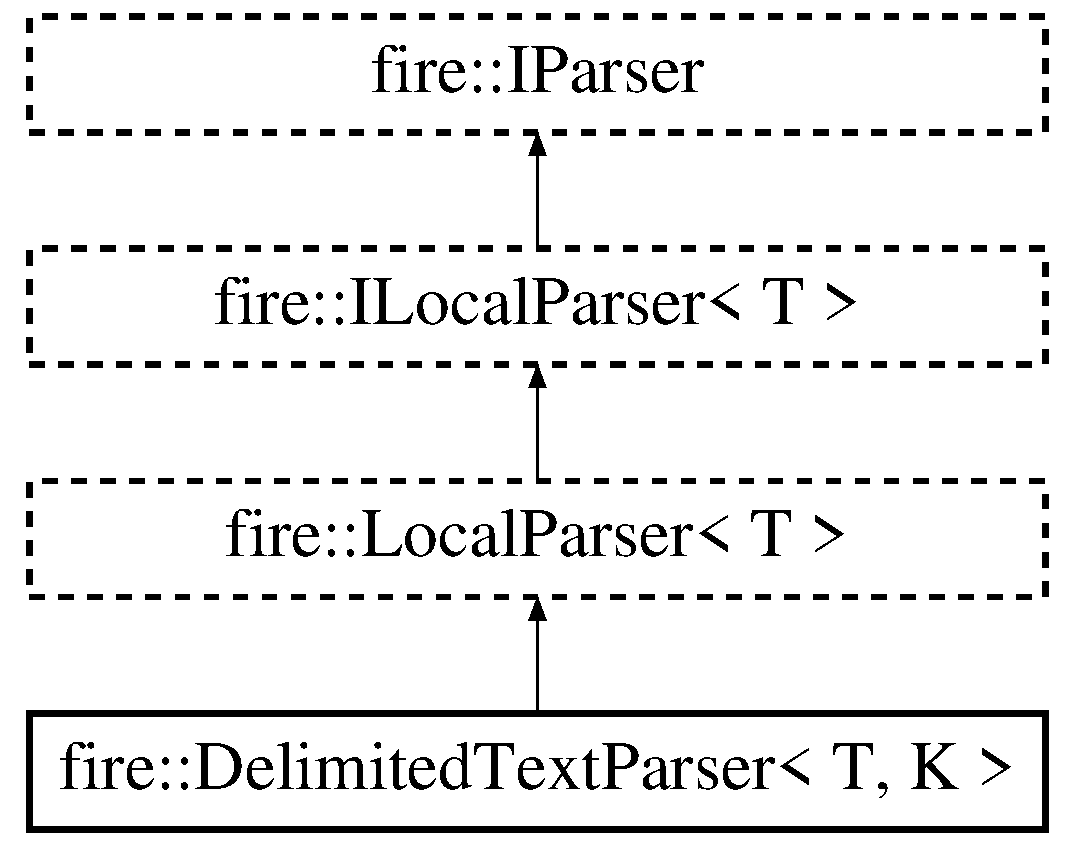
\includegraphics[height=4.000000cm]{a00008}
\end{center}
\end{figure}
\subsection*{Public Member Functions}
\begin{DoxyCompactItemize}
\item 
{\bfseries Delimited\+Text\+Parser} (string delim, string comment)\hypertarget{a00008_aa1f041ebbf0bf72145e8bd20bf95f3f4}{}\label{a00008_aa1f041ebbf0bf72145e8bd20bf95f3f4}

\item 
virtual void \hyperlink{a00008_a686df5548771cae833d5e721442a821a}{parse} ()
\item 
{\footnotesize template$<$$>$ }\\void \hyperlink{a00008_a773fa7ed28cb9d8c384ad94bd81fc93f}{parse} ()
\end{DoxyCompactItemize}
\subsection*{Protected Attributes}
\begin{DoxyCompactItemize}
\item 
string \hyperlink{a00008_ac817fc333b53611a41f446977461bdbf}{delimiter}
\item 
string \hyperlink{a00008_acdd7b27b8109ed41e7d9bc5e6de72e93}{comment\+Char}
\end{DoxyCompactItemize}


\subsection{Detailed Description}
\subsubsection*{template$<$typename T, typename K$>$\\*
class fire\+::\+Delimited\+Text\+Parser$<$ T, K $>$}

This class implements \hyperlink{a00012}{I\+Local\+Parser} to provide a local, file-\/based, serially executed delimited text parser.

\hyperlink{a00012_a091d5cf56bf8f407854ef87f460b2958}{is\+File()} will return true if set\+Source(string) is used is\+Stream() will return true if set\+Source(istream) is used \hyperlink{a00012_a770acae6e216de3a9c7140a12de25d58}{is\+Local()} always returns true. \hyperlink{a00012_ad46898c516adcce38acbb4800dc9777b}{is\+Parallel()} always returns false.

Because delimited text is most often primitives, this class requires two template arguments. The first argument T is how the data should be returned and the second argument K is the root type of the delimited text, most likely a primitive. This would look something like


\begin{DoxyCode}
DelimitedTextParser<vector<vector<double>>,\textcolor{keywordtype}{double}>
\end{DoxyCode}


for a dense body of text like in a standard C\+SV file or D\+AT file where each column is composed of dense primitives.

The source may either be a file on the local filesystem or an input stream.

This is an extension of the parser interface that focuses on parsing delimited text. Delimited text is text with entries that are separated by a common pattern, such as a common or space.

The Comma-\/\+Separated Variables format is a delimited text format of the form

v1, v2, v3, v4

where each comma is the delimiter between the text values v1 through v4. A line of text with only spaces is also a delimited text format\+:

v1 v2 v3 v4

Delimited text parsers may assume that lines such as those above are terminated by ~\newline
. Like most other text formats, delimited text files may contain comments, which may be skipped by I\+Delimited\+Text\+Parsers. The characters that denote comments -\/ very commonly a \char`\"{}\#\char`\"{} or \char`\"{}//\char`\"{} -\/ may be passed to the constructor. 

\subsection{Member Function Documentation}
\index{fire\+::\+Delimited\+Text\+Parser@{fire\+::\+Delimited\+Text\+Parser}!parse@{parse}}
\index{parse@{parse}!fire\+::\+Delimited\+Text\+Parser@{fire\+::\+Delimited\+Text\+Parser}}
\subsubsection[{\texorpdfstring{parse()}{parse()}}]{\setlength{\rightskip}{0pt plus 5cm}template$<$typename T , typename K $>$ virtual void {\bf fire\+::\+Delimited\+Text\+Parser}$<$ T, K $>$\+::parse (
\begin{DoxyParamCaption}
{}
\end{DoxyParamCaption}
)\hspace{0.3cm}{\ttfamily [inline]}, {\ttfamily [virtual]}}\hypertarget{a00008_a686df5548771cae833d5e721442a821a}{}\label{a00008_a686df5548771cae833d5e721442a821a}
This operation directs the parser to parse its source. 

Reimplemented from \hyperlink{a00019_abd8929aea06c2dda40256d2e58236650}{fire\+::\+Local\+Parser$<$ T $>$}.

\index{fire\+::\+Delimited\+Text\+Parser@{fire\+::\+Delimited\+Text\+Parser}!parse@{parse}}
\index{parse@{parse}!fire\+::\+Delimited\+Text\+Parser@{fire\+::\+Delimited\+Text\+Parser}}
\subsubsection[{\texorpdfstring{parse()}{parse()}}]{\setlength{\rightskip}{0pt plus 5cm}template$<$$>$ void {\bf fire\+::\+Delimited\+Text\+Parser}$<$ vector$<$ vector$<$ double $>$ $>$, double $>$\+::parse (
\begin{DoxyParamCaption}
{}
\end{DoxyParamCaption}
)\hspace{0.3cm}{\ttfamily [virtual]}}\hypertarget{a00008_a773fa7ed28cb9d8c384ad94bd81fc93f}{}\label{a00008_a773fa7ed28cb9d8c384ad94bd81fc93f}
This specialization is for dense data of primitive type double. 

Reimplemented from \hyperlink{a00019_abd8929aea06c2dda40256d2e58236650}{fire\+::\+Local\+Parser$<$ T $>$}.



\subsection{Member Data Documentation}
\index{fire\+::\+Delimited\+Text\+Parser@{fire\+::\+Delimited\+Text\+Parser}!comment\+Char@{comment\+Char}}
\index{comment\+Char@{comment\+Char}!fire\+::\+Delimited\+Text\+Parser@{fire\+::\+Delimited\+Text\+Parser}}
\subsubsection[{\texorpdfstring{comment\+Char}{commentChar}}]{\setlength{\rightskip}{0pt plus 5cm}template$<$typename T , typename K $>$ string {\bf fire\+::\+Delimited\+Text\+Parser}$<$ T, K $>$\+::comment\+Char\hspace{0.3cm}{\ttfamily [protected]}}\hypertarget{a00008_acdd7b27b8109ed41e7d9bc5e6de72e93}{}\label{a00008_acdd7b27b8109ed41e7d9bc5e6de72e93}
The character that represents a comment and should be skipped. \index{fire\+::\+Delimited\+Text\+Parser@{fire\+::\+Delimited\+Text\+Parser}!delimiter@{delimiter}}
\index{delimiter@{delimiter}!fire\+::\+Delimited\+Text\+Parser@{fire\+::\+Delimited\+Text\+Parser}}
\subsubsection[{\texorpdfstring{delimiter}{delimiter}}]{\setlength{\rightskip}{0pt plus 5cm}template$<$typename T , typename K $>$ string {\bf fire\+::\+Delimited\+Text\+Parser}$<$ T, K $>$\+::delimiter\hspace{0.3cm}{\ttfamily [protected]}}\hypertarget{a00008_ac817fc333b53611a41f446977461bdbf}{}\label{a00008_ac817fc333b53611a41f446977461bdbf}
The delimiter used when parsing the file. 

The documentation for this class was generated from the following file\+:\begin{DoxyCompactItemize}
\item 
Delimited\+Text\+Parser.\+h\end{DoxyCompactItemize}

\hypertarget{a00009}{}\section{Block\+Generator Struct Reference}
\label{a00009}\index{Block\+Generator@{Block\+Generator}}


The documentation for this struct was generated from the following file\+:\begin{DoxyCompactItemize}
\item 
I\+N\+I\+Property\+Parser\+Test.\+cpp\end{DoxyCompactItemize}

\hypertarget{a00010}{}\section{File\+Generator Struct Reference}
\label{a00010}\index{File\+Generator@{File\+Generator}}


The documentation for this struct was generated from the following file\+:\begin{DoxyCompactItemize}
\item 
Delimited\+Text\+Parser\+Test.\+cpp\end{DoxyCompactItemize}

\hypertarget{a00011}{}\section{C\+Simple\+Ini\+Templ$<$ S\+I\+\_\+\+C\+H\+A\+R, S\+I\+\_\+\+S\+T\+R\+L\+E\+S\+S, S\+I\+\_\+\+C\+O\+N\+V\+E\+R\+T\+E\+R $>$ Class Template Reference}
\label{a00011}\index{C\+Simple\+Ini\+Templ$<$ S\+I\+\_\+\+C\+H\+A\+R, S\+I\+\_\+\+S\+T\+R\+L\+E\+S\+S, S\+I\+\_\+\+C\+O\+N\+V\+E\+R\+T\+E\+R $>$@{C\+Simple\+Ini\+Templ$<$ S\+I\+\_\+\+C\+H\+A\+R, S\+I\+\_\+\+S\+T\+R\+L\+E\+S\+S, S\+I\+\_\+\+C\+O\+N\+V\+E\+R\+T\+E\+R $>$}}


{\ttfamily \#include $<$Simple\+Ini.\+h$>$}

\subsection*{Classes}
\begin{DoxyCompactItemize}
\item 
class \hyperlink{a00010}{Converter}
\item 
struct \hyperlink{a00015}{Entry}
\item 
class \hyperlink{a00017}{File\+Writer}
\item 
class \hyperlink{a00030}{Output\+Writer}
\item 
class \hyperlink{a00045}{String\+Writer}
\end{DoxyCompactItemize}
\subsection*{Public Types}
\begin{DoxyCompactItemize}
\item 
\hypertarget{a00011_ad7ffad7e87da2303a05b885e95bc74fa}{}typedef S\+I\+\_\+\+C\+H\+A\+R {\bfseries S\+I\+\_\+\+C\+H\+A\+R\+\_\+\+T}\label{a00011_ad7ffad7e87da2303a05b885e95bc74fa}

\item 
typedef std\+::multimap$<$ \hyperlink{a00015}{Entry}, const S\+I\+\_\+\+C\+H\+A\+R $\ast$, typename \hyperlink{a00027}{Entry\+::\+Key\+Order} $>$ \hyperlink{a00011_ae7f0e11d84617214bd479de6332c80e6}{T\+Key\+Val}
\item 
typedef std\+::map$<$ \hyperlink{a00015}{Entry}, \hyperlink{a00011_ae7f0e11d84617214bd479de6332c80e6}{T\+Key\+Val}, typename \hyperlink{a00027}{Entry\+::\+Key\+Order} $>$ \hyperlink{a00011_a2e7963455f680abd0d6901786495a665}{T\+Section}
\item 
typedef std\+::list$<$ \hyperlink{a00015}{Entry} $>$ \hyperlink{a00011_a391b3f3751e06cd9e9de4fb16ac14342}{T\+Names\+Depend}
\end{DoxyCompactItemize}
\subsection*{Public Member Functions}
\begin{DoxyCompactItemize}
\item 
\hyperlink{a00011_af878d0a2aa780255b621e95f58f691d8}{C\+Simple\+Ini\+Templ} (bool a\+\_\+b\+Is\+Utf8=false, bool a\+\_\+b\+Multi\+Key=false, bool a\+\_\+b\+Multi\+Line=false)
\item 
\hyperlink{a00011_a8c933adc1d46bb663caeb6f9dee5aa12}{$\sim$\+C\+Simple\+Ini\+Templ} ()
\item 
void \hyperlink{a00011_a89b34d38be4518e9ed91c634a41b8055}{Reset} ()
\item 
bool \hyperlink{a00011_acaada2b1ab734fc7dd8780ba7f376c26}{Is\+Empty} () const 
\item 
S\+I\+\_\+\+Error \hyperlink{a00011_aebb6e5fff76efc05ca6cc4b7b56481a3}{Load\+File} (const char $\ast$a\+\_\+psz\+File)
\item 
S\+I\+\_\+\+Error \hyperlink{a00011_a7ccb65e82fa347b42b59330968f826ae}{Load\+File} (F\+I\+L\+E $\ast$a\+\_\+fp\+File)
\item 
S\+I\+\_\+\+Error \hyperlink{a00011_a174244fd3e09ff78da05fe46be86e714}{Load\+Data} (const std\+::string \&a\+\_\+str\+Data)
\item 
S\+I\+\_\+\+Error \hyperlink{a00011_aa797cf47cec05906f07d5065882af4d3}{Load\+Data} (const char $\ast$a\+\_\+p\+Data, size\+\_\+t a\+\_\+u\+Data\+Len)
\item 
S\+I\+\_\+\+Error \hyperlink{a00011_a1449e083d968790ef7479de24edddba0}{Save\+File} (const char $\ast$a\+\_\+psz\+File, bool a\+\_\+b\+Add\+Signature=true) const 
\item 
S\+I\+\_\+\+Error \hyperlink{a00011_af3f26b331a0f9d7f071d7b4aa8038758}{Save\+File} (F\+I\+L\+E $\ast$a\+\_\+p\+File, bool a\+\_\+b\+Add\+Signature=false) const 
\item 
S\+I\+\_\+\+Error \hyperlink{a00011_a5fea5d590edbb5eef694991c7c355915}{Save} (\hyperlink{a00030}{Output\+Writer} \&a\+\_\+o\+Output, bool a\+\_\+b\+Add\+Signature=false) const 
\item 
S\+I\+\_\+\+Error \hyperlink{a00011_af944674fb44473ede150a3bcdc103d63}{Save} (std\+::string \&a\+\_\+s\+Buffer, bool a\+\_\+b\+Add\+Signature=false) const 
\item 
void \hyperlink{a00011_a65b01b5bf88d0dfe3ba51f12278cbcb8}{Get\+All\+Sections} (\hyperlink{a00011_a391b3f3751e06cd9e9de4fb16ac14342}{T\+Names\+Depend} \&a\+\_\+names) const 
\item 
bool \hyperlink{a00011_a8cf1357d78d28653b68790ab5d5b45f1}{Get\+All\+Keys} (const S\+I\+\_\+\+C\+H\+A\+R $\ast$a\+\_\+p\+Section, \hyperlink{a00011_a391b3f3751e06cd9e9de4fb16ac14342}{T\+Names\+Depend} \&a\+\_\+names) const 
\item 
bool \hyperlink{a00011_a263c85a8cd839c315fefc078e048257b}{Get\+All\+Values} (const S\+I\+\_\+\+C\+H\+A\+R $\ast$a\+\_\+p\+Section, const S\+I\+\_\+\+C\+H\+A\+R $\ast$a\+\_\+p\+Key, \hyperlink{a00011_a391b3f3751e06cd9e9de4fb16ac14342}{T\+Names\+Depend} \&a\+\_\+values) const 
\item 
int \hyperlink{a00011_a2e612d67d1e1631c157af6291ac8c348}{Get\+Section\+Size} (const S\+I\+\_\+\+C\+H\+A\+R $\ast$a\+\_\+p\+Section) const 
\item 
const \hyperlink{a00011_ae7f0e11d84617214bd479de6332c80e6}{T\+Key\+Val} $\ast$ \hyperlink{a00011_a795e2fcbad3472055aedfe188f4f8d33}{Get\+Section} (const S\+I\+\_\+\+C\+H\+A\+R $\ast$a\+\_\+p\+Section) const 
\item 
const S\+I\+\_\+\+C\+H\+A\+R $\ast$ \hyperlink{a00011_a39999339113e9395d5e2c6b02ef5c618}{Get\+Value} (const S\+I\+\_\+\+C\+H\+A\+R $\ast$a\+\_\+p\+Section, const S\+I\+\_\+\+C\+H\+A\+R $\ast$a\+\_\+p\+Key, const S\+I\+\_\+\+C\+H\+A\+R $\ast$a\+\_\+p\+Default=N\+U\+L\+L, bool $\ast$a\+\_\+p\+Has\+Multiple=N\+U\+L\+L) const 
\item 
long \hyperlink{a00011_a994c6b29bb8b4c16a4b1a7f4c8b2b3f4}{Get\+Long\+Value} (const S\+I\+\_\+\+C\+H\+A\+R $\ast$a\+\_\+p\+Section, const S\+I\+\_\+\+C\+H\+A\+R $\ast$a\+\_\+p\+Key, long a\+\_\+n\+Default=0, bool $\ast$a\+\_\+p\+Has\+Multiple=N\+U\+L\+L) const 
\item 
double \hyperlink{a00011_a6ce7c77a1d5d64dc289927a5c2659e78}{Get\+Double\+Value} (const S\+I\+\_\+\+C\+H\+A\+R $\ast$a\+\_\+p\+Section, const S\+I\+\_\+\+C\+H\+A\+R $\ast$a\+\_\+p\+Key, double a\+\_\+n\+Default=0, bool $\ast$a\+\_\+p\+Has\+Multiple=N\+U\+L\+L) const 
\item 
bool \hyperlink{a00011_af0a8cffb0b7f6ca04e3eed9ab4660666}{Get\+Bool\+Value} (const S\+I\+\_\+\+C\+H\+A\+R $\ast$a\+\_\+p\+Section, const S\+I\+\_\+\+C\+H\+A\+R $\ast$a\+\_\+p\+Key, bool a\+\_\+b\+Default=false, bool $\ast$a\+\_\+p\+Has\+Multiple=N\+U\+L\+L) const 
\item 
S\+I\+\_\+\+Error \hyperlink{a00011_aa2014a3dc8fdd638316cf1d3611796ab}{Set\+Value} (const S\+I\+\_\+\+C\+H\+A\+R $\ast$a\+\_\+p\+Section, const S\+I\+\_\+\+C\+H\+A\+R $\ast$a\+\_\+p\+Key, const S\+I\+\_\+\+C\+H\+A\+R $\ast$a\+\_\+p\+Value, const S\+I\+\_\+\+C\+H\+A\+R $\ast$a\+\_\+p\+Comment=N\+U\+L\+L, bool a\+\_\+b\+Force\+Replace=false)
\item 
S\+I\+\_\+\+Error \hyperlink{a00011_ab2238be407232e4bba0f1343e4793e4e}{Set\+Long\+Value} (const S\+I\+\_\+\+C\+H\+A\+R $\ast$a\+\_\+p\+Section, const S\+I\+\_\+\+C\+H\+A\+R $\ast$a\+\_\+p\+Key, long a\+\_\+n\+Value, const S\+I\+\_\+\+C\+H\+A\+R $\ast$a\+\_\+p\+Comment=N\+U\+L\+L, bool a\+\_\+b\+Use\+Hex=false, bool a\+\_\+b\+Force\+Replace=false)
\item 
S\+I\+\_\+\+Error \hyperlink{a00011_af92ba0b8067553ab693c62a370de6534}{Set\+Double\+Value} (const S\+I\+\_\+\+C\+H\+A\+R $\ast$a\+\_\+p\+Section, const S\+I\+\_\+\+C\+H\+A\+R $\ast$a\+\_\+p\+Key, double a\+\_\+n\+Value, const S\+I\+\_\+\+C\+H\+A\+R $\ast$a\+\_\+p\+Comment=N\+U\+L\+L, bool a\+\_\+b\+Force\+Replace=false)
\item 
S\+I\+\_\+\+Error \hyperlink{a00011_a48ae136fa20c5d7eb7ab0b75342b27cf}{Set\+Bool\+Value} (const S\+I\+\_\+\+C\+H\+A\+R $\ast$a\+\_\+p\+Section, const S\+I\+\_\+\+C\+H\+A\+R $\ast$a\+\_\+p\+Key, bool a\+\_\+b\+Value, const S\+I\+\_\+\+C\+H\+A\+R $\ast$a\+\_\+p\+Comment=N\+U\+L\+L, bool a\+\_\+b\+Force\+Replace=false)
\item 
bool \hyperlink{a00011_aa5c1cdd0b306434d9e9f1422888049da}{Delete} (const S\+I\+\_\+\+C\+H\+A\+R $\ast$a\+\_\+p\+Section, const S\+I\+\_\+\+C\+H\+A\+R $\ast$a\+\_\+p\+Key, bool a\+\_\+b\+Remove\+Empty=false)
\item 
\hyperlink{a00010}{Converter} \hyperlink{a00011_a98442d01db35187f2770f0a91042cce8}{Get\+Converter} () const 
\end{DoxyCompactItemize}
\begin{Indent}{\bf Settings}\par
\begin{DoxyCompactItemize}
\item 
void \hyperlink{a00011_aa9a15a66de893571014f661f89cb4d4b}{Set\+Unicode} (bool a\+\_\+b\+Is\+Utf8=true)
\item 
bool \hyperlink{a00011_aa18f29d67107392a9e9f361def892c71}{Is\+Unicode} () const 
\item 
void \hyperlink{a00011_ac3cfaf072a64f960bdcb7ddf2edc52b6}{Set\+Multi\+Key} (bool a\+\_\+b\+Allow\+Multi\+Key=true)
\item 
bool \hyperlink{a00011_a8069b3c574949b78fe0274ae803f0685}{Is\+Multi\+Key} () const 
\item 
void \hyperlink{a00011_aa7214b76600790053a5c715e9730aab0}{Set\+Multi\+Line} (bool a\+\_\+b\+Allow\+Multi\+Line=true)
\item 
bool \hyperlink{a00011_a805dba3689efd63f8c4485a5f2e89090}{Is\+Multi\+Line} () const 
\item 
void \hyperlink{a00011_ae3c0eae2dcd84a42c99bb86ae103662c}{Set\+Spaces} (bool a\+\_\+b\+Spaces=true)
\item 
bool \hyperlink{a00011_a9c967faf796cf5babea67e97975bed9b}{Using\+Spaces} () const 
\end{DoxyCompactItemize}
\end{Indent}


\subsection{Detailed Description}
\subsubsection*{template$<$class S\+I\+\_\+\+C\+H\+A\+R, class S\+I\+\_\+\+S\+T\+R\+L\+E\+S\+S, class S\+I\+\_\+\+C\+O\+N\+V\+E\+R\+T\+E\+R$>$class C\+Simple\+Ini\+Templ$<$ S\+I\+\_\+\+C\+H\+A\+R, S\+I\+\_\+\+S\+T\+R\+L\+E\+S\+S, S\+I\+\_\+\+C\+O\+N\+V\+E\+R\+T\+E\+R $>$}

Simple I\+N\+I file reader.

This can be instantiated with the choice of unicode or native characterset, and case sensitive or insensitive comparisons of section and key names. The supported combinations are pre-\/defined with the following typedefs\+:

\begin{TabularC}{3}
\hline
\rowcolor{lightgray}{\bf Interface }&{\bf Case-\/sensitive }&{\bf Typedef }\\\cline{1-3}
char &No &C\+Simple\+Ini\+A \\\cline{1-3}
char &Yes &C\+Simple\+Ini\+Case\+A \\\cline{1-3}
wchar\+\_\+t &No &C\+Simple\+Ini\+W \\\cline{1-3}
wchar\+\_\+t &Yes &C\+Simple\+Ini\+Case\+W \\\cline{1-3}
\end{TabularC}


Note that using other types for the S\+I\+\_\+\+C\+H\+A\+R is supported. For instance, unsigned char, unsigned short, etc. Note that where the alternative type is a different size to char/wchar\+\_\+t you may need to supply new helper classes for S\+I\+\_\+\+S\+T\+R\+L\+E\+S\+S and S\+I\+\_\+\+C\+O\+N\+V\+E\+R\+T\+E\+R. 

\subsection{Member Typedef Documentation}
\hypertarget{a00011_ae7f0e11d84617214bd479de6332c80e6}{}\index{C\+Simple\+Ini\+Templ@{C\+Simple\+Ini\+Templ}!T\+Key\+Val@{T\+Key\+Val}}
\index{T\+Key\+Val@{T\+Key\+Val}!C\+Simple\+Ini\+Templ@{C\+Simple\+Ini\+Templ}}
\subsubsection[{T\+Key\+Val}]{\setlength{\rightskip}{0pt plus 5cm}template$<$class S\+I\+\_\+\+C\+H\+A\+R , class S\+I\+\_\+\+S\+T\+R\+L\+E\+S\+S , class S\+I\+\_\+\+C\+O\+N\+V\+E\+R\+T\+E\+R $>$ typedef std\+::multimap$<${\bf Entry},const S\+I\+\_\+\+C\+H\+A\+R $\ast$,typename {\bf Entry\+::\+Key\+Order}$>$ {\bf C\+Simple\+Ini\+Templ}$<$ S\+I\+\_\+\+C\+H\+A\+R, S\+I\+\_\+\+S\+T\+R\+L\+E\+S\+S, S\+I\+\_\+\+C\+O\+N\+V\+E\+R\+T\+E\+R $>$\+::{\bf T\+Key\+Val}}\label{a00011_ae7f0e11d84617214bd479de6332c80e6}
map keys to values \hypertarget{a00011_a391b3f3751e06cd9e9de4fb16ac14342}{}\index{C\+Simple\+Ini\+Templ@{C\+Simple\+Ini\+Templ}!T\+Names\+Depend@{T\+Names\+Depend}}
\index{T\+Names\+Depend@{T\+Names\+Depend}!C\+Simple\+Ini\+Templ@{C\+Simple\+Ini\+Templ}}
\subsubsection[{T\+Names\+Depend}]{\setlength{\rightskip}{0pt plus 5cm}template$<$class S\+I\+\_\+\+C\+H\+A\+R , class S\+I\+\_\+\+S\+T\+R\+L\+E\+S\+S , class S\+I\+\_\+\+C\+O\+N\+V\+E\+R\+T\+E\+R $>$ typedef std\+::list$<${\bf Entry}$>$ {\bf C\+Simple\+Ini\+Templ}$<$ S\+I\+\_\+\+C\+H\+A\+R, S\+I\+\_\+\+S\+T\+R\+L\+E\+S\+S, S\+I\+\_\+\+C\+O\+N\+V\+E\+R\+T\+E\+R $>$\+::{\bf T\+Names\+Depend}}\label{a00011_a391b3f3751e06cd9e9de4fb16ac14342}
set of dependent string pointers. Note that these pointers are dependent on memory owned by C\+Simple\+Ini. \hypertarget{a00011_a2e7963455f680abd0d6901786495a665}{}\index{C\+Simple\+Ini\+Templ@{C\+Simple\+Ini\+Templ}!T\+Section@{T\+Section}}
\index{T\+Section@{T\+Section}!C\+Simple\+Ini\+Templ@{C\+Simple\+Ini\+Templ}}
\subsubsection[{T\+Section}]{\setlength{\rightskip}{0pt plus 5cm}template$<$class S\+I\+\_\+\+C\+H\+A\+R , class S\+I\+\_\+\+S\+T\+R\+L\+E\+S\+S , class S\+I\+\_\+\+C\+O\+N\+V\+E\+R\+T\+E\+R $>$ typedef std\+::map$<${\bf Entry},{\bf T\+Key\+Val},typename {\bf Entry\+::\+Key\+Order}$>$ {\bf C\+Simple\+Ini\+Templ}$<$ S\+I\+\_\+\+C\+H\+A\+R, S\+I\+\_\+\+S\+T\+R\+L\+E\+S\+S, S\+I\+\_\+\+C\+O\+N\+V\+E\+R\+T\+E\+R $>$\+::{\bf T\+Section}}\label{a00011_a2e7963455f680abd0d6901786495a665}
map sections to key/value map 

\subsection{Constructor \& Destructor Documentation}
\hypertarget{a00011_af878d0a2aa780255b621e95f58f691d8}{}\index{C\+Simple\+Ini\+Templ@{C\+Simple\+Ini\+Templ}!C\+Simple\+Ini\+Templ@{C\+Simple\+Ini\+Templ}}
\index{C\+Simple\+Ini\+Templ@{C\+Simple\+Ini\+Templ}!C\+Simple\+Ini\+Templ@{C\+Simple\+Ini\+Templ}}
\subsubsection[{C\+Simple\+Ini\+Templ(bool a\+\_\+b\+Is\+Utf8=false, bool a\+\_\+b\+Multi\+Key=false, bool a\+\_\+b\+Multi\+Line=false)}]{\setlength{\rightskip}{0pt plus 5cm}template$<$class S\+I\+\_\+\+C\+H\+A\+R , class S\+I\+\_\+\+S\+T\+R\+L\+E\+S\+S , class S\+I\+\_\+\+C\+O\+N\+V\+E\+R\+T\+E\+R $>$ {\bf C\+Simple\+Ini\+Templ}$<$ S\+I\+\_\+\+C\+H\+A\+R, S\+I\+\_\+\+S\+T\+R\+L\+E\+S\+S, S\+I\+\_\+\+C\+O\+N\+V\+E\+R\+T\+E\+R $>$\+::{\bf C\+Simple\+Ini\+Templ} (
\begin{DoxyParamCaption}
\item[{bool}]{a\+\_\+b\+Is\+Utf8 = {\ttfamily false}, }
\item[{bool}]{a\+\_\+b\+Multi\+Key = {\ttfamily false}, }
\item[{bool}]{a\+\_\+b\+Multi\+Line = {\ttfamily false}}
\end{DoxyParamCaption}
)}\label{a00011_af878d0a2aa780255b621e95f58f691d8}
Default constructor.


\begin{DoxyParams}{Parameters}
{\em a\+\_\+b\+Is\+Utf8} & See the method \hyperlink{a00011_aa9a15a66de893571014f661f89cb4d4b}{Set\+Unicode()} for details. \\
\hline
{\em a\+\_\+b\+Multi\+Key} & See the method \hyperlink{a00011_ac3cfaf072a64f960bdcb7ddf2edc52b6}{Set\+Multi\+Key()} for details. \\
\hline
{\em a\+\_\+b\+Multi\+Line} & See the method \hyperlink{a00011_aa7214b76600790053a5c715e9730aab0}{Set\+Multi\+Line()} for details. \\
\hline
\end{DoxyParams}
\hypertarget{a00011_a8c933adc1d46bb663caeb6f9dee5aa12}{}\index{C\+Simple\+Ini\+Templ@{C\+Simple\+Ini\+Templ}!````~C\+Simple\+Ini\+Templ@{$\sim$\+C\+Simple\+Ini\+Templ}}
\index{````~C\+Simple\+Ini\+Templ@{$\sim$\+C\+Simple\+Ini\+Templ}!C\+Simple\+Ini\+Templ@{C\+Simple\+Ini\+Templ}}
\subsubsection[{$\sim$\+C\+Simple\+Ini\+Templ()}]{\setlength{\rightskip}{0pt plus 5cm}template$<$class S\+I\+\_\+\+C\+H\+A\+R , class S\+I\+\_\+\+S\+T\+R\+L\+E\+S\+S , class S\+I\+\_\+\+C\+O\+N\+V\+E\+R\+T\+E\+R $>$ {\bf C\+Simple\+Ini\+Templ}$<$ S\+I\+\_\+\+C\+H\+A\+R, S\+I\+\_\+\+S\+T\+R\+L\+E\+S\+S, S\+I\+\_\+\+C\+O\+N\+V\+E\+R\+T\+E\+R $>$\+::$\sim${\bf C\+Simple\+Ini\+Templ} (
\begin{DoxyParamCaption}
{}
\end{DoxyParamCaption}
)}\label{a00011_a8c933adc1d46bb663caeb6f9dee5aa12}
Destructor 

\subsection{Member Function Documentation}
\hypertarget{a00011_aa5c1cdd0b306434d9e9f1422888049da}{}\index{C\+Simple\+Ini\+Templ@{C\+Simple\+Ini\+Templ}!Delete@{Delete}}
\index{Delete@{Delete}!C\+Simple\+Ini\+Templ@{C\+Simple\+Ini\+Templ}}
\subsubsection[{Delete(const S\+I\+\_\+\+C\+H\+A\+R $\ast$a\+\_\+p\+Section, const S\+I\+\_\+\+C\+H\+A\+R $\ast$a\+\_\+p\+Key, bool a\+\_\+b\+Remove\+Empty=false)}]{\setlength{\rightskip}{0pt plus 5cm}template$<$class S\+I\+\_\+\+C\+H\+A\+R , class S\+I\+\_\+\+S\+T\+R\+L\+E\+S\+S , class S\+I\+\_\+\+C\+O\+N\+V\+E\+R\+T\+E\+R $>$ bool {\bf C\+Simple\+Ini\+Templ}$<$ S\+I\+\_\+\+C\+H\+A\+R, S\+I\+\_\+\+S\+T\+R\+L\+E\+S\+S, S\+I\+\_\+\+C\+O\+N\+V\+E\+R\+T\+E\+R $>$\+::Delete (
\begin{DoxyParamCaption}
\item[{const S\+I\+\_\+\+C\+H\+A\+R $\ast$}]{a\+\_\+p\+Section, }
\item[{const S\+I\+\_\+\+C\+H\+A\+R $\ast$}]{a\+\_\+p\+Key, }
\item[{bool}]{a\+\_\+b\+Remove\+Empty = {\ttfamily false}}
\end{DoxyParamCaption}
)}\label{a00011_aa5c1cdd0b306434d9e9f1422888049da}
Delete an entire section, or a key from a section. Note that the data returned by Get\+Section is invalid and must not be used after anything has been deleted from that section using this method. Note when multiple keys is enabled, this will delete all keys with that name; there is no way to selectively delete individual key/values in this situation.


\begin{DoxyParams}{Parameters}
{\em a\+\_\+p\+Section} & Section to delete key from, or if a\+\_\+p\+Key is N\+U\+L\+L, the section to remove. \\
\hline
{\em a\+\_\+p\+Key} & Key to remove from the section. Set to N\+U\+L\+L to remove the entire section. \\
\hline
{\em a\+\_\+b\+Remove\+Empty} & If the section is empty after this key has been deleted, should the empty section be removed?\\
\hline
\end{DoxyParams}
\begin{DoxyReturn}{Returns}
true Key or section was deleted. 

false Key or section was not found. 
\end{DoxyReturn}
\hypertarget{a00011_a8cf1357d78d28653b68790ab5d5b45f1}{}\index{C\+Simple\+Ini\+Templ@{C\+Simple\+Ini\+Templ}!Get\+All\+Keys@{Get\+All\+Keys}}
\index{Get\+All\+Keys@{Get\+All\+Keys}!C\+Simple\+Ini\+Templ@{C\+Simple\+Ini\+Templ}}
\subsubsection[{Get\+All\+Keys(const S\+I\+\_\+\+C\+H\+A\+R $\ast$a\+\_\+p\+Section, T\+Names\+Depend \&a\+\_\+names) const }]{\setlength{\rightskip}{0pt plus 5cm}template$<$class S\+I\+\_\+\+C\+H\+A\+R , class S\+I\+\_\+\+S\+T\+R\+L\+E\+S\+S , class S\+I\+\_\+\+C\+O\+N\+V\+E\+R\+T\+E\+R $>$ bool {\bf C\+Simple\+Ini\+Templ}$<$ S\+I\+\_\+\+C\+H\+A\+R, S\+I\+\_\+\+S\+T\+R\+L\+E\+S\+S, S\+I\+\_\+\+C\+O\+N\+V\+E\+R\+T\+E\+R $>$\+::Get\+All\+Keys (
\begin{DoxyParamCaption}
\item[{const S\+I\+\_\+\+C\+H\+A\+R $\ast$}]{a\+\_\+p\+Section, }
\item[{{\bf T\+Names\+Depend} \&}]{a\+\_\+names}
\end{DoxyParamCaption}
) const}\label{a00011_a8cf1357d78d28653b68790ab5d5b45f1}
Retrieve all unique key names in a section. The sort order of the returned strings is N\+O\+T D\+E\+F\+I\+N\+E\+D. You can sort the names into the load order if desired. Search this file for \char`\"{}.\+sort\char`\"{} for an example. Only unique key names are returned.

N\+O\+T\+E! This structure contains only pointers to strings. The actual string data is stored in memory owned by C\+Simple\+Ini. Ensure that the C\+Simple\+Ini object is not destroyed or \hyperlink{a00011_a89b34d38be4518e9ed91c634a41b8055}{Reset()} while these strings are in use!


\begin{DoxyParams}{Parameters}
{\em a\+\_\+p\+Section} & Section to request data for \\
\hline
{\em a\+\_\+names} & List that will receive all of the key names. See note above!\\
\hline
\end{DoxyParams}
\begin{DoxyReturn}{Returns}
true Section was found. 

false Matching section was not found. 
\end{DoxyReturn}
\hypertarget{a00011_a65b01b5bf88d0dfe3ba51f12278cbcb8}{}\index{C\+Simple\+Ini\+Templ@{C\+Simple\+Ini\+Templ}!Get\+All\+Sections@{Get\+All\+Sections}}
\index{Get\+All\+Sections@{Get\+All\+Sections}!C\+Simple\+Ini\+Templ@{C\+Simple\+Ini\+Templ}}
\subsubsection[{Get\+All\+Sections(\+T\+Names\+Depend \&a\+\_\+names) const }]{\setlength{\rightskip}{0pt plus 5cm}template$<$class S\+I\+\_\+\+C\+H\+A\+R , class S\+I\+\_\+\+S\+T\+R\+L\+E\+S\+S , class S\+I\+\_\+\+C\+O\+N\+V\+E\+R\+T\+E\+R $>$ void {\bf C\+Simple\+Ini\+Templ}$<$ S\+I\+\_\+\+C\+H\+A\+R, S\+I\+\_\+\+S\+T\+R\+L\+E\+S\+S, S\+I\+\_\+\+C\+O\+N\+V\+E\+R\+T\+E\+R $>$\+::Get\+All\+Sections (
\begin{DoxyParamCaption}
\item[{{\bf T\+Names\+Depend} \&}]{a\+\_\+names}
\end{DoxyParamCaption}
) const}\label{a00011_a65b01b5bf88d0dfe3ba51f12278cbcb8}
Retrieve all section names. The list is returned as an S\+T\+L vector of names and can be iterated or searched as necessary. Note that the sort order of the returned strings is N\+O\+T D\+E\+F\+I\+N\+E\+D. You can sort the names into the load order if desired. Search this file for \char`\"{}.\+sort\char`\"{} for an example.

N\+O\+T\+E! This structure contains only pointers to strings. The actual string data is stored in memory owned by C\+Simple\+Ini. Ensure that the C\+Simple\+Ini object is not destroyed or \hyperlink{a00011_a89b34d38be4518e9ed91c634a41b8055}{Reset()} while these pointers are in use!


\begin{DoxyParams}{Parameters}
{\em a\+\_\+names} & Vector that will receive all of the section names. See note above! \\
\hline
\end{DoxyParams}
\hypertarget{a00011_a263c85a8cd839c315fefc078e048257b}{}\index{C\+Simple\+Ini\+Templ@{C\+Simple\+Ini\+Templ}!Get\+All\+Values@{Get\+All\+Values}}
\index{Get\+All\+Values@{Get\+All\+Values}!C\+Simple\+Ini\+Templ@{C\+Simple\+Ini\+Templ}}
\subsubsection[{Get\+All\+Values(const S\+I\+\_\+\+C\+H\+A\+R $\ast$a\+\_\+p\+Section, const S\+I\+\_\+\+C\+H\+A\+R $\ast$a\+\_\+p\+Key, T\+Names\+Depend \&a\+\_\+values) const }]{\setlength{\rightskip}{0pt plus 5cm}template$<$class S\+I\+\_\+\+C\+H\+A\+R , class S\+I\+\_\+\+S\+T\+R\+L\+E\+S\+S , class S\+I\+\_\+\+C\+O\+N\+V\+E\+R\+T\+E\+R $>$ bool {\bf C\+Simple\+Ini\+Templ}$<$ S\+I\+\_\+\+C\+H\+A\+R, S\+I\+\_\+\+S\+T\+R\+L\+E\+S\+S, S\+I\+\_\+\+C\+O\+N\+V\+E\+R\+T\+E\+R $>$\+::Get\+All\+Values (
\begin{DoxyParamCaption}
\item[{const S\+I\+\_\+\+C\+H\+A\+R $\ast$}]{a\+\_\+p\+Section, }
\item[{const S\+I\+\_\+\+C\+H\+A\+R $\ast$}]{a\+\_\+p\+Key, }
\item[{{\bf T\+Names\+Depend} \&}]{a\+\_\+values}
\end{DoxyParamCaption}
) const}\label{a00011_a263c85a8cd839c315fefc078e048257b}
Retrieve all values for a specific key. This method can be used when multiple keys are both enabled and disabled. Note that the sort order of the returned strings is N\+O\+T D\+E\+F\+I\+N\+E\+D. You can sort the names into the load order if desired. Search this file for \char`\"{}.\+sort\char`\"{} for an example.

N\+O\+T\+E! The returned values are pointers to string data stored in memory owned by C\+Simple\+Ini. Ensure that the C\+Simple\+Ini object is not destroyed or Reset while you are using this pointer!


\begin{DoxyParams}{Parameters}
{\em a\+\_\+p\+Section} & Section to search \\
\hline
{\em a\+\_\+p\+Key} & Key to search for \\
\hline
{\em a\+\_\+values} & List to return if the key is not found\\
\hline
\end{DoxyParams}
\begin{DoxyReturn}{Returns}
true Key was found. 

false Matching section/key was not found. 
\end{DoxyReturn}
\hypertarget{a00011_af0a8cffb0b7f6ca04e3eed9ab4660666}{}\index{C\+Simple\+Ini\+Templ@{C\+Simple\+Ini\+Templ}!Get\+Bool\+Value@{Get\+Bool\+Value}}
\index{Get\+Bool\+Value@{Get\+Bool\+Value}!C\+Simple\+Ini\+Templ@{C\+Simple\+Ini\+Templ}}
\subsubsection[{Get\+Bool\+Value(const S\+I\+\_\+\+C\+H\+A\+R $\ast$a\+\_\+p\+Section, const S\+I\+\_\+\+C\+H\+A\+R $\ast$a\+\_\+p\+Key, bool a\+\_\+b\+Default=false, bool $\ast$a\+\_\+p\+Has\+Multiple=\+N\+U\+L\+L) const }]{\setlength{\rightskip}{0pt plus 5cm}template$<$class S\+I\+\_\+\+C\+H\+A\+R , class S\+I\+\_\+\+S\+T\+R\+L\+E\+S\+S , class S\+I\+\_\+\+C\+O\+N\+V\+E\+R\+T\+E\+R $>$ bool {\bf C\+Simple\+Ini\+Templ}$<$ S\+I\+\_\+\+C\+H\+A\+R, S\+I\+\_\+\+S\+T\+R\+L\+E\+S\+S, S\+I\+\_\+\+C\+O\+N\+V\+E\+R\+T\+E\+R $>$\+::Get\+Bool\+Value (
\begin{DoxyParamCaption}
\item[{const S\+I\+\_\+\+C\+H\+A\+R $\ast$}]{a\+\_\+p\+Section, }
\item[{const S\+I\+\_\+\+C\+H\+A\+R $\ast$}]{a\+\_\+p\+Key, }
\item[{bool}]{a\+\_\+b\+Default = {\ttfamily false}, }
\item[{bool $\ast$}]{a\+\_\+p\+Has\+Multiple = {\ttfamily NULL}}
\end{DoxyParamCaption}
) const}\label{a00011_af0a8cffb0b7f6ca04e3eed9ab4660666}
Retrieve a boolean value for a specific key. If multiple keys are enabled (see Set\+Multi\+Key) then only the first value associated with that key will be returned, see Get\+All\+Values for getting all values with multikey.

Strings starting with \char`\"{}t\char`\"{}, \char`\"{}y\char`\"{}, \char`\"{}on\char`\"{} or \char`\"{}1\char`\"{} are returned as logically true. Strings starting with \char`\"{}f\char`\"{}, \char`\"{}n\char`\"{}, \char`\"{}of\char`\"{} or \char`\"{}0\char`\"{} are returned as logically false. For all other values the default is returned. Character comparisons are case-\/insensitive.


\begin{DoxyParams}{Parameters}
{\em a\+\_\+p\+Section} & Section to search \\
\hline
{\em a\+\_\+p\+Key} & Key to search for \\
\hline
{\em a\+\_\+b\+Default} & Value to return if the key is not found \\
\hline
{\em a\+\_\+p\+Has\+Multiple} & Optionally receive notification of if there are multiple entries for this key.\\
\hline
\end{DoxyParams}
\begin{DoxyReturn}{Returns}
a\+\_\+n\+Default Key was not found in the section 

other Value of the key 
\end{DoxyReturn}
\hypertarget{a00011_a98442d01db35187f2770f0a91042cce8}{}\index{C\+Simple\+Ini\+Templ@{C\+Simple\+Ini\+Templ}!Get\+Converter@{Get\+Converter}}
\index{Get\+Converter@{Get\+Converter}!C\+Simple\+Ini\+Templ@{C\+Simple\+Ini\+Templ}}
\subsubsection[{Get\+Converter() const }]{\setlength{\rightskip}{0pt plus 5cm}template$<$class S\+I\+\_\+\+C\+H\+A\+R , class S\+I\+\_\+\+S\+T\+R\+L\+E\+S\+S , class S\+I\+\_\+\+C\+O\+N\+V\+E\+R\+T\+E\+R $>$ {\bf Converter} {\bf C\+Simple\+Ini\+Templ}$<$ S\+I\+\_\+\+C\+H\+A\+R, S\+I\+\_\+\+S\+T\+R\+L\+E\+S\+S, S\+I\+\_\+\+C\+O\+N\+V\+E\+R\+T\+E\+R $>$\+::Get\+Converter (
\begin{DoxyParamCaption}
{}
\end{DoxyParamCaption}
) const\hspace{0.3cm}{\ttfamily [inline]}}\label{a00011_a98442d01db35187f2770f0a91042cce8}
Return a conversion object to convert text to the same encoding as is used by the \hyperlink{a00011_a5fea5d590edbb5eef694991c7c355915}{Save()}, \hyperlink{a00011_a1449e083d968790ef7479de24edddba0}{Save\+File()} and Save\+String() functions. Use this to prepare the strings that you wish to append or prepend to the output I\+N\+I data. \hypertarget{a00011_a6ce7c77a1d5d64dc289927a5c2659e78}{}\index{C\+Simple\+Ini\+Templ@{C\+Simple\+Ini\+Templ}!Get\+Double\+Value@{Get\+Double\+Value}}
\index{Get\+Double\+Value@{Get\+Double\+Value}!C\+Simple\+Ini\+Templ@{C\+Simple\+Ini\+Templ}}
\subsubsection[{Get\+Double\+Value(const S\+I\+\_\+\+C\+H\+A\+R $\ast$a\+\_\+p\+Section, const S\+I\+\_\+\+C\+H\+A\+R $\ast$a\+\_\+p\+Key, double a\+\_\+n\+Default=0, bool $\ast$a\+\_\+p\+Has\+Multiple=\+N\+U\+L\+L) const }]{\setlength{\rightskip}{0pt plus 5cm}template$<$class S\+I\+\_\+\+C\+H\+A\+R , class S\+I\+\_\+\+S\+T\+R\+L\+E\+S\+S , class S\+I\+\_\+\+C\+O\+N\+V\+E\+R\+T\+E\+R $>$ double {\bf C\+Simple\+Ini\+Templ}$<$ S\+I\+\_\+\+C\+H\+A\+R, S\+I\+\_\+\+S\+T\+R\+L\+E\+S\+S, S\+I\+\_\+\+C\+O\+N\+V\+E\+R\+T\+E\+R $>$\+::Get\+Double\+Value (
\begin{DoxyParamCaption}
\item[{const S\+I\+\_\+\+C\+H\+A\+R $\ast$}]{a\+\_\+p\+Section, }
\item[{const S\+I\+\_\+\+C\+H\+A\+R $\ast$}]{a\+\_\+p\+Key, }
\item[{double}]{a\+\_\+n\+Default = {\ttfamily 0}, }
\item[{bool $\ast$}]{a\+\_\+p\+Has\+Multiple = {\ttfamily NULL}}
\end{DoxyParamCaption}
) const}\label{a00011_a6ce7c77a1d5d64dc289927a5c2659e78}
Retrieve a numeric value for a specific key. If multiple keys are enabled (see Set\+Multi\+Key) then only the first value associated with that key will be returned, see Get\+All\+Values for getting all values with multikey.


\begin{DoxyParams}{Parameters}
{\em a\+\_\+p\+Section} & Section to search \\
\hline
{\em a\+\_\+p\+Key} & Key to search for \\
\hline
{\em a\+\_\+n\+Default} & Value to return if the key is not found \\
\hline
{\em a\+\_\+p\+Has\+Multiple} & Optionally receive notification of if there are multiple entries for this key.\\
\hline
\end{DoxyParams}
\begin{DoxyReturn}{Returns}
a\+\_\+n\+Default Key was not found in the section 

other Value of the key 
\end{DoxyReturn}
\hypertarget{a00011_a994c6b29bb8b4c16a4b1a7f4c8b2b3f4}{}\index{C\+Simple\+Ini\+Templ@{C\+Simple\+Ini\+Templ}!Get\+Long\+Value@{Get\+Long\+Value}}
\index{Get\+Long\+Value@{Get\+Long\+Value}!C\+Simple\+Ini\+Templ@{C\+Simple\+Ini\+Templ}}
\subsubsection[{Get\+Long\+Value(const S\+I\+\_\+\+C\+H\+A\+R $\ast$a\+\_\+p\+Section, const S\+I\+\_\+\+C\+H\+A\+R $\ast$a\+\_\+p\+Key, long a\+\_\+n\+Default=0, bool $\ast$a\+\_\+p\+Has\+Multiple=\+N\+U\+L\+L) const }]{\setlength{\rightskip}{0pt plus 5cm}template$<$class S\+I\+\_\+\+C\+H\+A\+R , class S\+I\+\_\+\+S\+T\+R\+L\+E\+S\+S , class S\+I\+\_\+\+C\+O\+N\+V\+E\+R\+T\+E\+R $>$ long {\bf C\+Simple\+Ini\+Templ}$<$ S\+I\+\_\+\+C\+H\+A\+R, S\+I\+\_\+\+S\+T\+R\+L\+E\+S\+S, S\+I\+\_\+\+C\+O\+N\+V\+E\+R\+T\+E\+R $>$\+::Get\+Long\+Value (
\begin{DoxyParamCaption}
\item[{const S\+I\+\_\+\+C\+H\+A\+R $\ast$}]{a\+\_\+p\+Section, }
\item[{const S\+I\+\_\+\+C\+H\+A\+R $\ast$}]{a\+\_\+p\+Key, }
\item[{long}]{a\+\_\+n\+Default = {\ttfamily 0}, }
\item[{bool $\ast$}]{a\+\_\+p\+Has\+Multiple = {\ttfamily NULL}}
\end{DoxyParamCaption}
) const}\label{a00011_a994c6b29bb8b4c16a4b1a7f4c8b2b3f4}
Retrieve a numeric value for a specific key. If multiple keys are enabled (see Set\+Multi\+Key) then only the first value associated with that key will be returned, see Get\+All\+Values for getting all values with multikey.


\begin{DoxyParams}{Parameters}
{\em a\+\_\+p\+Section} & Section to search \\
\hline
{\em a\+\_\+p\+Key} & Key to search for \\
\hline
{\em a\+\_\+n\+Default} & Value to return if the key is not found \\
\hline
{\em a\+\_\+p\+Has\+Multiple} & Optionally receive notification of if there are multiple entries for this key.\\
\hline
\end{DoxyParams}
\begin{DoxyReturn}{Returns}
a\+\_\+n\+Default Key was not found in the section 

other Value of the key 
\end{DoxyReturn}
\hypertarget{a00011_a795e2fcbad3472055aedfe188f4f8d33}{}\index{C\+Simple\+Ini\+Templ@{C\+Simple\+Ini\+Templ}!Get\+Section@{Get\+Section}}
\index{Get\+Section@{Get\+Section}!C\+Simple\+Ini\+Templ@{C\+Simple\+Ini\+Templ}}
\subsubsection[{Get\+Section(const S\+I\+\_\+\+C\+H\+A\+R $\ast$a\+\_\+p\+Section) const }]{\setlength{\rightskip}{0pt plus 5cm}template$<$class S\+I\+\_\+\+C\+H\+A\+R , class S\+I\+\_\+\+S\+T\+R\+L\+E\+S\+S , class S\+I\+\_\+\+C\+O\+N\+V\+E\+R\+T\+E\+R $>$ const {\bf C\+Simple\+Ini\+Templ}$<$ S\+I\+\_\+\+C\+H\+A\+R, S\+I\+\_\+\+S\+T\+R\+L\+E\+S\+S, S\+I\+\_\+\+C\+O\+N\+V\+E\+R\+T\+E\+R $>$\+::{\bf T\+Key\+Val} $\ast$ {\bf C\+Simple\+Ini\+Templ}$<$ S\+I\+\_\+\+C\+H\+A\+R, S\+I\+\_\+\+S\+T\+R\+L\+E\+S\+S, S\+I\+\_\+\+C\+O\+N\+V\+E\+R\+T\+E\+R $>$\+::Get\+Section (
\begin{DoxyParamCaption}
\item[{const S\+I\+\_\+\+C\+H\+A\+R $\ast$}]{a\+\_\+p\+Section}
\end{DoxyParamCaption}
) const}\label{a00011_a795e2fcbad3472055aedfe188f4f8d33}
Retrieve all key and value pairs for a section. The data is returned as a pointer to an S\+T\+L map and can be iterated or searched as desired. Note that multiple entries for the same key may exist when multiple keys have been enabled.

N\+O\+T\+E! This structure contains only pointers to strings. The actual string data is stored in memory owned by C\+Simple\+Ini. Ensure that the C\+Simple\+Ini object is not destroyed or \hyperlink{a00011_a89b34d38be4518e9ed91c634a41b8055}{Reset()} while these strings are in use!


\begin{DoxyParams}{Parameters}
{\em a\+\_\+p\+Section} & Name of the section to return \\
\hline
\end{DoxyParams}
\begin{DoxyReturn}{Returns}
boolean Was a section matching the supplied name found. 
\end{DoxyReturn}
\hypertarget{a00011_a2e612d67d1e1631c157af6291ac8c348}{}\index{C\+Simple\+Ini\+Templ@{C\+Simple\+Ini\+Templ}!Get\+Section\+Size@{Get\+Section\+Size}}
\index{Get\+Section\+Size@{Get\+Section\+Size}!C\+Simple\+Ini\+Templ@{C\+Simple\+Ini\+Templ}}
\subsubsection[{Get\+Section\+Size(const S\+I\+\_\+\+C\+H\+A\+R $\ast$a\+\_\+p\+Section) const }]{\setlength{\rightskip}{0pt plus 5cm}template$<$class S\+I\+\_\+\+C\+H\+A\+R , class S\+I\+\_\+\+S\+T\+R\+L\+E\+S\+S , class S\+I\+\_\+\+C\+O\+N\+V\+E\+R\+T\+E\+R $>$ int {\bf C\+Simple\+Ini\+Templ}$<$ S\+I\+\_\+\+C\+H\+A\+R, S\+I\+\_\+\+S\+T\+R\+L\+E\+S\+S, S\+I\+\_\+\+C\+O\+N\+V\+E\+R\+T\+E\+R $>$\+::Get\+Section\+Size (
\begin{DoxyParamCaption}
\item[{const S\+I\+\_\+\+C\+H\+A\+R $\ast$}]{a\+\_\+p\+Section}
\end{DoxyParamCaption}
) const}\label{a00011_a2e612d67d1e1631c157af6291ac8c348}
Query the number of keys in a specific section. Note that if multiple keys are enabled, then this value may be different to the number of keys returned by Get\+All\+Keys.


\begin{DoxyParams}{Parameters}
{\em a\+\_\+p\+Section} & Section to request data for\\
\hline
\end{DoxyParams}
\begin{DoxyReturn}{Returns}
-\/1 Section does not exist in the file 

$>$=0 Number of keys in the section 
\end{DoxyReturn}
\hypertarget{a00011_a39999339113e9395d5e2c6b02ef5c618}{}\index{C\+Simple\+Ini\+Templ@{C\+Simple\+Ini\+Templ}!Get\+Value@{Get\+Value}}
\index{Get\+Value@{Get\+Value}!C\+Simple\+Ini\+Templ@{C\+Simple\+Ini\+Templ}}
\subsubsection[{Get\+Value(const S\+I\+\_\+\+C\+H\+A\+R $\ast$a\+\_\+p\+Section, const S\+I\+\_\+\+C\+H\+A\+R $\ast$a\+\_\+p\+Key, const S\+I\+\_\+\+C\+H\+A\+R $\ast$a\+\_\+p\+Default=\+N\+U\+L\+L, bool $\ast$a\+\_\+p\+Has\+Multiple=\+N\+U\+L\+L) const }]{\setlength{\rightskip}{0pt plus 5cm}template$<$class S\+I\+\_\+\+C\+H\+A\+R , class S\+I\+\_\+\+S\+T\+R\+L\+E\+S\+S , class S\+I\+\_\+\+C\+O\+N\+V\+E\+R\+T\+E\+R $>$ const S\+I\+\_\+\+C\+H\+A\+R $\ast$ {\bf C\+Simple\+Ini\+Templ}$<$ S\+I\+\_\+\+C\+H\+A\+R, S\+I\+\_\+\+S\+T\+R\+L\+E\+S\+S, S\+I\+\_\+\+C\+O\+N\+V\+E\+R\+T\+E\+R $>$\+::Get\+Value (
\begin{DoxyParamCaption}
\item[{const S\+I\+\_\+\+C\+H\+A\+R $\ast$}]{a\+\_\+p\+Section, }
\item[{const S\+I\+\_\+\+C\+H\+A\+R $\ast$}]{a\+\_\+p\+Key, }
\item[{const S\+I\+\_\+\+C\+H\+A\+R $\ast$}]{a\+\_\+p\+Default = {\ttfamily NULL}, }
\item[{bool $\ast$}]{a\+\_\+p\+Has\+Multiple = {\ttfamily NULL}}
\end{DoxyParamCaption}
) const}\label{a00011_a39999339113e9395d5e2c6b02ef5c618}
Retrieve the value for a specific key. If multiple keys are enabled (see Set\+Multi\+Key) then only the first value associated with that key will be returned, see Get\+All\+Values for getting all values with multikey.

N\+O\+T\+E! The returned value is a pointer to string data stored in memory owned by C\+Simple\+Ini. Ensure that the C\+Simple\+Ini object is not destroyed or Reset while you are using this pointer!


\begin{DoxyParams}{Parameters}
{\em a\+\_\+p\+Section} & Section to search \\
\hline
{\em a\+\_\+p\+Key} & Key to search for \\
\hline
{\em a\+\_\+p\+Default} & Value to return if the key is not found \\
\hline
{\em a\+\_\+p\+Has\+Multiple} & Optionally receive notification of if there are multiple entries for this key.\\
\hline
\end{DoxyParams}
\begin{DoxyReturn}{Returns}
a\+\_\+p\+Default Key was not found in the section 

other Value of the key 
\end{DoxyReturn}
\hypertarget{a00011_acaada2b1ab734fc7dd8780ba7f376c26}{}\index{C\+Simple\+Ini\+Templ@{C\+Simple\+Ini\+Templ}!Is\+Empty@{Is\+Empty}}
\index{Is\+Empty@{Is\+Empty}!C\+Simple\+Ini\+Templ@{C\+Simple\+Ini\+Templ}}
\subsubsection[{Is\+Empty() const }]{\setlength{\rightskip}{0pt plus 5cm}template$<$class S\+I\+\_\+\+C\+H\+A\+R , class S\+I\+\_\+\+S\+T\+R\+L\+E\+S\+S , class S\+I\+\_\+\+C\+O\+N\+V\+E\+R\+T\+E\+R $>$ bool {\bf C\+Simple\+Ini\+Templ}$<$ S\+I\+\_\+\+C\+H\+A\+R, S\+I\+\_\+\+S\+T\+R\+L\+E\+S\+S, S\+I\+\_\+\+C\+O\+N\+V\+E\+R\+T\+E\+R $>$\+::Is\+Empty (
\begin{DoxyParamCaption}
{}
\end{DoxyParamCaption}
) const\hspace{0.3cm}{\ttfamily [inline]}}\label{a00011_acaada2b1ab734fc7dd8780ba7f376c26}
Has any data been loaded \hypertarget{a00011_a8069b3c574949b78fe0274ae803f0685}{}\index{C\+Simple\+Ini\+Templ@{C\+Simple\+Ini\+Templ}!Is\+Multi\+Key@{Is\+Multi\+Key}}
\index{Is\+Multi\+Key@{Is\+Multi\+Key}!C\+Simple\+Ini\+Templ@{C\+Simple\+Ini\+Templ}}
\subsubsection[{Is\+Multi\+Key() const }]{\setlength{\rightskip}{0pt plus 5cm}template$<$class S\+I\+\_\+\+C\+H\+A\+R , class S\+I\+\_\+\+S\+T\+R\+L\+E\+S\+S , class S\+I\+\_\+\+C\+O\+N\+V\+E\+R\+T\+E\+R $>$ bool {\bf C\+Simple\+Ini\+Templ}$<$ S\+I\+\_\+\+C\+H\+A\+R, S\+I\+\_\+\+S\+T\+R\+L\+E\+S\+S, S\+I\+\_\+\+C\+O\+N\+V\+E\+R\+T\+E\+R $>$\+::Is\+Multi\+Key (
\begin{DoxyParamCaption}
{}
\end{DoxyParamCaption}
) const\hspace{0.3cm}{\ttfamily [inline]}}\label{a00011_a8069b3c574949b78fe0274ae803f0685}
Get the storage format of the I\+N\+I data. \hypertarget{a00011_a805dba3689efd63f8c4485a5f2e89090}{}\index{C\+Simple\+Ini\+Templ@{C\+Simple\+Ini\+Templ}!Is\+Multi\+Line@{Is\+Multi\+Line}}
\index{Is\+Multi\+Line@{Is\+Multi\+Line}!C\+Simple\+Ini\+Templ@{C\+Simple\+Ini\+Templ}}
\subsubsection[{Is\+Multi\+Line() const }]{\setlength{\rightskip}{0pt plus 5cm}template$<$class S\+I\+\_\+\+C\+H\+A\+R , class S\+I\+\_\+\+S\+T\+R\+L\+E\+S\+S , class S\+I\+\_\+\+C\+O\+N\+V\+E\+R\+T\+E\+R $>$ bool {\bf C\+Simple\+Ini\+Templ}$<$ S\+I\+\_\+\+C\+H\+A\+R, S\+I\+\_\+\+S\+T\+R\+L\+E\+S\+S, S\+I\+\_\+\+C\+O\+N\+V\+E\+R\+T\+E\+R $>$\+::Is\+Multi\+Line (
\begin{DoxyParamCaption}
{}
\end{DoxyParamCaption}
) const\hspace{0.3cm}{\ttfamily [inline]}}\label{a00011_a805dba3689efd63f8c4485a5f2e89090}
Query the status of multi-\/line data \hypertarget{a00011_aa18f29d67107392a9e9f361def892c71}{}\index{C\+Simple\+Ini\+Templ@{C\+Simple\+Ini\+Templ}!Is\+Unicode@{Is\+Unicode}}
\index{Is\+Unicode@{Is\+Unicode}!C\+Simple\+Ini\+Templ@{C\+Simple\+Ini\+Templ}}
\subsubsection[{Is\+Unicode() const }]{\setlength{\rightskip}{0pt plus 5cm}template$<$class S\+I\+\_\+\+C\+H\+A\+R , class S\+I\+\_\+\+S\+T\+R\+L\+E\+S\+S , class S\+I\+\_\+\+C\+O\+N\+V\+E\+R\+T\+E\+R $>$ bool {\bf C\+Simple\+Ini\+Templ}$<$ S\+I\+\_\+\+C\+H\+A\+R, S\+I\+\_\+\+S\+T\+R\+L\+E\+S\+S, S\+I\+\_\+\+C\+O\+N\+V\+E\+R\+T\+E\+R $>$\+::Is\+Unicode (
\begin{DoxyParamCaption}
{}
\end{DoxyParamCaption}
) const\hspace{0.3cm}{\ttfamily [inline]}}\label{a00011_aa18f29d67107392a9e9f361def892c71}
Get the storage format of the I\+N\+I data. \hypertarget{a00011_a174244fd3e09ff78da05fe46be86e714}{}\index{C\+Simple\+Ini\+Templ@{C\+Simple\+Ini\+Templ}!Load\+Data@{Load\+Data}}
\index{Load\+Data@{Load\+Data}!C\+Simple\+Ini\+Templ@{C\+Simple\+Ini\+Templ}}
\subsubsection[{Load\+Data(const std\+::string \&a\+\_\+str\+Data)}]{\setlength{\rightskip}{0pt plus 5cm}template$<$class S\+I\+\_\+\+C\+H\+A\+R , class S\+I\+\_\+\+S\+T\+R\+L\+E\+S\+S , class S\+I\+\_\+\+C\+O\+N\+V\+E\+R\+T\+E\+R $>$ S\+I\+\_\+\+Error {\bf C\+Simple\+Ini\+Templ}$<$ S\+I\+\_\+\+C\+H\+A\+R, S\+I\+\_\+\+S\+T\+R\+L\+E\+S\+S, S\+I\+\_\+\+C\+O\+N\+V\+E\+R\+T\+E\+R $>$\+::Load\+Data (
\begin{DoxyParamCaption}
\item[{const std\+::string \&}]{a\+\_\+str\+Data}
\end{DoxyParamCaption}
)\hspace{0.3cm}{\ttfamily [inline]}}\label{a00011_a174244fd3e09ff78da05fe46be86e714}
Load I\+N\+I file data direct from a std\+::string


\begin{DoxyParams}{Parameters}
{\em a\+\_\+str\+Data} & Data to be loaded\\
\hline
\end{DoxyParams}
\begin{DoxyReturn}{Returns}
S\+I\+\_\+\+Error See error definitions 
\end{DoxyReturn}
\hypertarget{a00011_aa797cf47cec05906f07d5065882af4d3}{}\index{C\+Simple\+Ini\+Templ@{C\+Simple\+Ini\+Templ}!Load\+Data@{Load\+Data}}
\index{Load\+Data@{Load\+Data}!C\+Simple\+Ini\+Templ@{C\+Simple\+Ini\+Templ}}
\subsubsection[{Load\+Data(const char $\ast$a\+\_\+p\+Data, size\+\_\+t a\+\_\+u\+Data\+Len)}]{\setlength{\rightskip}{0pt plus 5cm}template$<$class S\+I\+\_\+\+C\+H\+A\+R , class S\+I\+\_\+\+S\+T\+R\+L\+E\+S\+S , class S\+I\+\_\+\+C\+O\+N\+V\+E\+R\+T\+E\+R $>$ S\+I\+\_\+\+Error {\bf C\+Simple\+Ini\+Templ}$<$ S\+I\+\_\+\+C\+H\+A\+R, S\+I\+\_\+\+S\+T\+R\+L\+E\+S\+S, S\+I\+\_\+\+C\+O\+N\+V\+E\+R\+T\+E\+R $>$\+::Load\+Data (
\begin{DoxyParamCaption}
\item[{const char $\ast$}]{a\+\_\+p\+Data, }
\item[{size\+\_\+t}]{a\+\_\+u\+Data\+Len}
\end{DoxyParamCaption}
)}\label{a00011_aa797cf47cec05906f07d5065882af4d3}
Load I\+N\+I file data direct from memory


\begin{DoxyParams}{Parameters}
{\em a\+\_\+p\+Data} & Data to be loaded \\
\hline
{\em a\+\_\+u\+Data\+Len} & Length of the data in bytes\\
\hline
\end{DoxyParams}
\begin{DoxyReturn}{Returns}
S\+I\+\_\+\+Error See error definitions 
\end{DoxyReturn}
\hypertarget{a00011_aebb6e5fff76efc05ca6cc4b7b56481a3}{}\index{C\+Simple\+Ini\+Templ@{C\+Simple\+Ini\+Templ}!Load\+File@{Load\+File}}
\index{Load\+File@{Load\+File}!C\+Simple\+Ini\+Templ@{C\+Simple\+Ini\+Templ}}
\subsubsection[{Load\+File(const char $\ast$a\+\_\+psz\+File)}]{\setlength{\rightskip}{0pt plus 5cm}template$<$class S\+I\+\_\+\+C\+H\+A\+R , class S\+I\+\_\+\+S\+T\+R\+L\+E\+S\+S , class S\+I\+\_\+\+C\+O\+N\+V\+E\+R\+T\+E\+R $>$ S\+I\+\_\+\+Error {\bf C\+Simple\+Ini\+Templ}$<$ S\+I\+\_\+\+C\+H\+A\+R, S\+I\+\_\+\+S\+T\+R\+L\+E\+S\+S, S\+I\+\_\+\+C\+O\+N\+V\+E\+R\+T\+E\+R $>$\+::Load\+File (
\begin{DoxyParamCaption}
\item[{const char $\ast$}]{a\+\_\+psz\+File}
\end{DoxyParamCaption}
)}\label{a00011_aebb6e5fff76efc05ca6cc4b7b56481a3}
Load an I\+N\+I file from disk into memory


\begin{DoxyParams}{Parameters}
{\em a\+\_\+psz\+File} & Path of the file to be loaded. This will be passed to fopen() and so must be a valid path for the current platform.\\
\hline
\end{DoxyParams}
\begin{DoxyReturn}{Returns}
S\+I\+\_\+\+Error See error definitions 
\end{DoxyReturn}
\hypertarget{a00011_a7ccb65e82fa347b42b59330968f826ae}{}\index{C\+Simple\+Ini\+Templ@{C\+Simple\+Ini\+Templ}!Load\+File@{Load\+File}}
\index{Load\+File@{Load\+File}!C\+Simple\+Ini\+Templ@{C\+Simple\+Ini\+Templ}}
\subsubsection[{Load\+File(\+F\+I\+L\+E $\ast$a\+\_\+fp\+File)}]{\setlength{\rightskip}{0pt plus 5cm}template$<$class S\+I\+\_\+\+C\+H\+A\+R , class S\+I\+\_\+\+S\+T\+R\+L\+E\+S\+S , class S\+I\+\_\+\+C\+O\+N\+V\+E\+R\+T\+E\+R $>$ S\+I\+\_\+\+Error {\bf C\+Simple\+Ini\+Templ}$<$ S\+I\+\_\+\+C\+H\+A\+R, S\+I\+\_\+\+S\+T\+R\+L\+E\+S\+S, S\+I\+\_\+\+C\+O\+N\+V\+E\+R\+T\+E\+R $>$\+::Load\+File (
\begin{DoxyParamCaption}
\item[{F\+I\+L\+E $\ast$}]{a\+\_\+fp\+File}
\end{DoxyParamCaption}
)}\label{a00011_a7ccb65e82fa347b42b59330968f826ae}
Load the file from a file pointer.


\begin{DoxyParams}{Parameters}
{\em a\+\_\+fp\+File} & Valid file pointer to read the file data from. The file will be read until end of file.\\
\hline
\end{DoxyParams}
\begin{DoxyReturn}{Returns}
S\+I\+\_\+\+Error See error definitions 
\end{DoxyReturn}
\hypertarget{a00011_a89b34d38be4518e9ed91c634a41b8055}{}\index{C\+Simple\+Ini\+Templ@{C\+Simple\+Ini\+Templ}!Reset@{Reset}}
\index{Reset@{Reset}!C\+Simple\+Ini\+Templ@{C\+Simple\+Ini\+Templ}}
\subsubsection[{Reset()}]{\setlength{\rightskip}{0pt plus 5cm}template$<$class S\+I\+\_\+\+C\+H\+A\+R , class S\+I\+\_\+\+S\+T\+R\+L\+E\+S\+S , class S\+I\+\_\+\+C\+O\+N\+V\+E\+R\+T\+E\+R $>$ void {\bf C\+Simple\+Ini\+Templ}$<$ S\+I\+\_\+\+C\+H\+A\+R, S\+I\+\_\+\+S\+T\+R\+L\+E\+S\+S, S\+I\+\_\+\+C\+O\+N\+V\+E\+R\+T\+E\+R $>$\+::Reset (
\begin{DoxyParamCaption}
{}
\end{DoxyParamCaption}
)}\label{a00011_a89b34d38be4518e9ed91c634a41b8055}
Deallocate all memory stored by this object \hypertarget{a00011_a5fea5d590edbb5eef694991c7c355915}{}\index{C\+Simple\+Ini\+Templ@{C\+Simple\+Ini\+Templ}!Save@{Save}}
\index{Save@{Save}!C\+Simple\+Ini\+Templ@{C\+Simple\+Ini\+Templ}}
\subsubsection[{Save(\+Output\+Writer \&a\+\_\+o\+Output, bool a\+\_\+b\+Add\+Signature=false) const }]{\setlength{\rightskip}{0pt plus 5cm}template$<$class S\+I\+\_\+\+C\+H\+A\+R , class S\+I\+\_\+\+S\+T\+R\+L\+E\+S\+S , class S\+I\+\_\+\+C\+O\+N\+V\+E\+R\+T\+E\+R $>$ S\+I\+\_\+\+Error {\bf C\+Simple\+Ini\+Templ}$<$ S\+I\+\_\+\+C\+H\+A\+R, S\+I\+\_\+\+S\+T\+R\+L\+E\+S\+S, S\+I\+\_\+\+C\+O\+N\+V\+E\+R\+T\+E\+R $>$\+::Save (
\begin{DoxyParamCaption}
\item[{{\bf Output\+Writer} \&}]{a\+\_\+o\+Output, }
\item[{bool}]{a\+\_\+b\+Add\+Signature = {\ttfamily false}}
\end{DoxyParamCaption}
) const}\label{a00011_a5fea5d590edbb5eef694991c7c355915}
Save the I\+N\+I data. The data will be written to the output device in a format appropriate to the current data, selected by\+:

\begin{TabularC}{2}
\hline
\rowcolor{lightgray}{\bf S\+I\+\_\+\+C\+H\+A\+R }&{\bf F\+O\+R\+M\+A\+T }\\\cline{1-2}
char &same format as when loaded (M\+B\+C\+S or U\+T\+F-\/8) \\\cline{1-2}
wchar\+\_\+t &U\+T\+F-\/8 \\\cline{1-2}
other &U\+T\+F-\/8 \\\cline{1-2}
\end{TabularC}


Note that comments from the original data is preserved as per the documentation on comments. The order of the sections and values from the original file will be preserved.

Any data prepended or appended to the output device must use the the same format (M\+B\+C\+S or U\+T\+F-\/8). You may use the \hyperlink{a00011_a98442d01db35187f2770f0a91042cce8}{Get\+Converter()} method to convert text to the correct format regardless of the output format being used by Simple\+Ini.

To add a B\+O\+M to U\+T\+F-\/8 data, write it out manually at the very beginning like is done in Save\+File when a\+\_\+b\+Use\+B\+O\+M is true.


\begin{DoxyParams}{Parameters}
{\em a\+\_\+o\+Output} & Output writer to write the data to.\\
\hline
{\em a\+\_\+b\+Add\+Signature} & Prepend the U\+T\+F-\/8 B\+O\+M if the output data is in U\+T\+F-\/8 format. If it is not U\+T\+F-\/8 then this value is ignored. Do not set this to true if anything has already been written to the \hyperlink{a00030}{Output\+Writer}.\\
\hline
\end{DoxyParams}
\begin{DoxyReturn}{Returns}
S\+I\+\_\+\+Error See error definitions 
\end{DoxyReturn}
\hypertarget{a00011_af944674fb44473ede150a3bcdc103d63}{}\index{C\+Simple\+Ini\+Templ@{C\+Simple\+Ini\+Templ}!Save@{Save}}
\index{Save@{Save}!C\+Simple\+Ini\+Templ@{C\+Simple\+Ini\+Templ}}
\subsubsection[{Save(std\+::string \&a\+\_\+s\+Buffer, bool a\+\_\+b\+Add\+Signature=false) const }]{\setlength{\rightskip}{0pt plus 5cm}template$<$class S\+I\+\_\+\+C\+H\+A\+R , class S\+I\+\_\+\+S\+T\+R\+L\+E\+S\+S , class S\+I\+\_\+\+C\+O\+N\+V\+E\+R\+T\+E\+R $>$ S\+I\+\_\+\+Error {\bf C\+Simple\+Ini\+Templ}$<$ S\+I\+\_\+\+C\+H\+A\+R, S\+I\+\_\+\+S\+T\+R\+L\+E\+S\+S, S\+I\+\_\+\+C\+O\+N\+V\+E\+R\+T\+E\+R $>$\+::Save (
\begin{DoxyParamCaption}
\item[{std\+::string \&}]{a\+\_\+s\+Buffer, }
\item[{bool}]{a\+\_\+b\+Add\+Signature = {\ttfamily false}}
\end{DoxyParamCaption}
) const\hspace{0.3cm}{\ttfamily [inline]}}\label{a00011_af944674fb44473ede150a3bcdc103d63}
Append the I\+N\+I data to a string. See \hyperlink{a00011_a5fea5d590edbb5eef694991c7c355915}{Save()} for details.


\begin{DoxyParams}{Parameters}
{\em a\+\_\+s\+Buffer} & String to have the I\+N\+I data appended to.\\
\hline
{\em a\+\_\+b\+Add\+Signature} & Prepend the U\+T\+F-\/8 B\+O\+M if the output data is in U\+T\+F-\/8 format. If it is not U\+T\+F-\/8 then this value is ignored. Do not set this to true if anything has already been written to the string.\\
\hline
\end{DoxyParams}
\begin{DoxyReturn}{Returns}
S\+I\+\_\+\+Error See error definitions 
\end{DoxyReturn}
\hypertarget{a00011_a1449e083d968790ef7479de24edddba0}{}\index{C\+Simple\+Ini\+Templ@{C\+Simple\+Ini\+Templ}!Save\+File@{Save\+File}}
\index{Save\+File@{Save\+File}!C\+Simple\+Ini\+Templ@{C\+Simple\+Ini\+Templ}}
\subsubsection[{Save\+File(const char $\ast$a\+\_\+psz\+File, bool a\+\_\+b\+Add\+Signature=true) const }]{\setlength{\rightskip}{0pt plus 5cm}template$<$class S\+I\+\_\+\+C\+H\+A\+R , class S\+I\+\_\+\+S\+T\+R\+L\+E\+S\+S , class S\+I\+\_\+\+C\+O\+N\+V\+E\+R\+T\+E\+R $>$ S\+I\+\_\+\+Error {\bf C\+Simple\+Ini\+Templ}$<$ S\+I\+\_\+\+C\+H\+A\+R, S\+I\+\_\+\+S\+T\+R\+L\+E\+S\+S, S\+I\+\_\+\+C\+O\+N\+V\+E\+R\+T\+E\+R $>$\+::Save\+File (
\begin{DoxyParamCaption}
\item[{const char $\ast$}]{a\+\_\+psz\+File, }
\item[{bool}]{a\+\_\+b\+Add\+Signature = {\ttfamily true}}
\end{DoxyParamCaption}
) const}\label{a00011_a1449e083d968790ef7479de24edddba0}
Save an I\+N\+I file from memory to disk


\begin{DoxyParams}{Parameters}
{\em a\+\_\+psz\+File} & Path of the file to be saved. This will be passed to fopen() and so must be a valid path for the current platform.\\
\hline
{\em a\+\_\+b\+Add\+Signature} & Prepend the U\+T\+F-\/8 B\+O\+M if the output data is in U\+T\+F-\/8 format. If it is not U\+T\+F-\/8 then this parameter is ignored.\\
\hline
\end{DoxyParams}
\begin{DoxyReturn}{Returns}
S\+I\+\_\+\+Error See error definitions 
\end{DoxyReturn}
\hypertarget{a00011_af3f26b331a0f9d7f071d7b4aa8038758}{}\index{C\+Simple\+Ini\+Templ@{C\+Simple\+Ini\+Templ}!Save\+File@{Save\+File}}
\index{Save\+File@{Save\+File}!C\+Simple\+Ini\+Templ@{C\+Simple\+Ini\+Templ}}
\subsubsection[{Save\+File(\+F\+I\+L\+E $\ast$a\+\_\+p\+File, bool a\+\_\+b\+Add\+Signature=false) const }]{\setlength{\rightskip}{0pt plus 5cm}template$<$class S\+I\+\_\+\+C\+H\+A\+R , class S\+I\+\_\+\+S\+T\+R\+L\+E\+S\+S , class S\+I\+\_\+\+C\+O\+N\+V\+E\+R\+T\+E\+R $>$ S\+I\+\_\+\+Error {\bf C\+Simple\+Ini\+Templ}$<$ S\+I\+\_\+\+C\+H\+A\+R, S\+I\+\_\+\+S\+T\+R\+L\+E\+S\+S, S\+I\+\_\+\+C\+O\+N\+V\+E\+R\+T\+E\+R $>$\+::Save\+File (
\begin{DoxyParamCaption}
\item[{F\+I\+L\+E $\ast$}]{a\+\_\+p\+File, }
\item[{bool}]{a\+\_\+b\+Add\+Signature = {\ttfamily false}}
\end{DoxyParamCaption}
) const}\label{a00011_af3f26b331a0f9d7f071d7b4aa8038758}
Save the I\+N\+I data to a file. See \hyperlink{a00011_a5fea5d590edbb5eef694991c7c355915}{Save()} for details.


\begin{DoxyParams}{Parameters}
{\em a\+\_\+p\+File} & Handle to a file. File should be opened for binary output.\\
\hline
{\em a\+\_\+b\+Add\+Signature} & Prepend the U\+T\+F-\/8 B\+O\+M if the output data is in U\+T\+F-\/8 format. If it is not U\+T\+F-\/8 then this value is ignored. Do not set this to true if anything has already been written to the file.\\
\hline
\end{DoxyParams}
\begin{DoxyReturn}{Returns}
S\+I\+\_\+\+Error See error definitions 
\end{DoxyReturn}
\hypertarget{a00011_a48ae136fa20c5d7eb7ab0b75342b27cf}{}\index{C\+Simple\+Ini\+Templ@{C\+Simple\+Ini\+Templ}!Set\+Bool\+Value@{Set\+Bool\+Value}}
\index{Set\+Bool\+Value@{Set\+Bool\+Value}!C\+Simple\+Ini\+Templ@{C\+Simple\+Ini\+Templ}}
\subsubsection[{Set\+Bool\+Value(const S\+I\+\_\+\+C\+H\+A\+R $\ast$a\+\_\+p\+Section, const S\+I\+\_\+\+C\+H\+A\+R $\ast$a\+\_\+p\+Key, bool a\+\_\+b\+Value, const S\+I\+\_\+\+C\+H\+A\+R $\ast$a\+\_\+p\+Comment=\+N\+U\+L\+L, bool a\+\_\+b\+Force\+Replace=false)}]{\setlength{\rightskip}{0pt plus 5cm}template$<$class S\+I\+\_\+\+C\+H\+A\+R , class S\+I\+\_\+\+S\+T\+R\+L\+E\+S\+S , class S\+I\+\_\+\+C\+O\+N\+V\+E\+R\+T\+E\+R $>$ S\+I\+\_\+\+Error {\bf C\+Simple\+Ini\+Templ}$<$ S\+I\+\_\+\+C\+H\+A\+R, S\+I\+\_\+\+S\+T\+R\+L\+E\+S\+S, S\+I\+\_\+\+C\+O\+N\+V\+E\+R\+T\+E\+R $>$\+::Set\+Bool\+Value (
\begin{DoxyParamCaption}
\item[{const S\+I\+\_\+\+C\+H\+A\+R $\ast$}]{a\+\_\+p\+Section, }
\item[{const S\+I\+\_\+\+C\+H\+A\+R $\ast$}]{a\+\_\+p\+Key, }
\item[{bool}]{a\+\_\+b\+Value, }
\item[{const S\+I\+\_\+\+C\+H\+A\+R $\ast$}]{a\+\_\+p\+Comment = {\ttfamily NULL}, }
\item[{bool}]{a\+\_\+b\+Force\+Replace = {\ttfamily false}}
\end{DoxyParamCaption}
)}\label{a00011_a48ae136fa20c5d7eb7ab0b75342b27cf}
Add or update a boolean value. This will always insert when multiple keys are enabled.


\begin{DoxyParams}{Parameters}
{\em a\+\_\+p\+Section} & Section to add or update \\
\hline
{\em a\+\_\+p\+Key} & Key to add or update. \\
\hline
{\em a\+\_\+b\+Value} & Value to set. \\
\hline
{\em a\+\_\+p\+Comment} & Comment to be associated with the key. See the notes on \hyperlink{a00011_aa2014a3dc8fdd638316cf1d3611796ab}{Set\+Value()} for comments. \\
\hline
{\em a\+\_\+b\+Force\+Replace} & Should all existing values in a multi-\/key I\+N\+I file be replaced with this entry. This option has no effect if not using multi-\/key files. The difference between Delete/\+Set\+Bool\+Value and Set\+Bool\+Value with a\+\_\+b\+Force\+Replace = true, is that the load order and comment will be preserved this way.\\
\hline
\end{DoxyParams}
\begin{DoxyReturn}{Returns}
S\+I\+\_\+\+Error See error definitions 

S\+I\+\_\+\+U\+P\+D\+A\+T\+E\+D Value was updated 

S\+I\+\_\+\+I\+N\+S\+E\+R\+T\+E\+D Value was inserted 
\end{DoxyReturn}
\hypertarget{a00011_af92ba0b8067553ab693c62a370de6534}{}\index{C\+Simple\+Ini\+Templ@{C\+Simple\+Ini\+Templ}!Set\+Double\+Value@{Set\+Double\+Value}}
\index{Set\+Double\+Value@{Set\+Double\+Value}!C\+Simple\+Ini\+Templ@{C\+Simple\+Ini\+Templ}}
\subsubsection[{Set\+Double\+Value(const S\+I\+\_\+\+C\+H\+A\+R $\ast$a\+\_\+p\+Section, const S\+I\+\_\+\+C\+H\+A\+R $\ast$a\+\_\+p\+Key, double a\+\_\+n\+Value, const S\+I\+\_\+\+C\+H\+A\+R $\ast$a\+\_\+p\+Comment=\+N\+U\+L\+L, bool a\+\_\+b\+Force\+Replace=false)}]{\setlength{\rightskip}{0pt plus 5cm}template$<$class S\+I\+\_\+\+C\+H\+A\+R , class S\+I\+\_\+\+S\+T\+R\+L\+E\+S\+S , class S\+I\+\_\+\+C\+O\+N\+V\+E\+R\+T\+E\+R $>$ S\+I\+\_\+\+Error {\bf C\+Simple\+Ini\+Templ}$<$ S\+I\+\_\+\+C\+H\+A\+R, S\+I\+\_\+\+S\+T\+R\+L\+E\+S\+S, S\+I\+\_\+\+C\+O\+N\+V\+E\+R\+T\+E\+R $>$\+::Set\+Double\+Value (
\begin{DoxyParamCaption}
\item[{const S\+I\+\_\+\+C\+H\+A\+R $\ast$}]{a\+\_\+p\+Section, }
\item[{const S\+I\+\_\+\+C\+H\+A\+R $\ast$}]{a\+\_\+p\+Key, }
\item[{double}]{a\+\_\+n\+Value, }
\item[{const S\+I\+\_\+\+C\+H\+A\+R $\ast$}]{a\+\_\+p\+Comment = {\ttfamily NULL}, }
\item[{bool}]{a\+\_\+b\+Force\+Replace = {\ttfamily false}}
\end{DoxyParamCaption}
)}\label{a00011_af92ba0b8067553ab693c62a370de6534}
Add or update a double value. This will always insert when multiple keys are enabled.


\begin{DoxyParams}{Parameters}
{\em a\+\_\+p\+Section} & Section to add or update \\
\hline
{\em a\+\_\+p\+Key} & Key to add or update. \\
\hline
{\em a\+\_\+n\+Value} & Value to set. \\
\hline
{\em a\+\_\+p\+Comment} & Comment to be associated with the key. See the notes on \hyperlink{a00011_aa2014a3dc8fdd638316cf1d3611796ab}{Set\+Value()} for comments. \\
\hline
{\em a\+\_\+b\+Force\+Replace} & Should all existing values in a multi-\/key I\+N\+I file be replaced with this entry. This option has no effect if not using multi-\/key files. The difference between Delete/\+Set\+Double\+Value and Set\+Double\+Value with a\+\_\+b\+Force\+Replace = true, is that the load order and comment will be preserved this way.\\
\hline
\end{DoxyParams}
\begin{DoxyReturn}{Returns}
S\+I\+\_\+\+Error See error definitions 

S\+I\+\_\+\+U\+P\+D\+A\+T\+E\+D Value was updated 

S\+I\+\_\+\+I\+N\+S\+E\+R\+T\+E\+D Value was inserted 
\end{DoxyReturn}
\hypertarget{a00011_ab2238be407232e4bba0f1343e4793e4e}{}\index{C\+Simple\+Ini\+Templ@{C\+Simple\+Ini\+Templ}!Set\+Long\+Value@{Set\+Long\+Value}}
\index{Set\+Long\+Value@{Set\+Long\+Value}!C\+Simple\+Ini\+Templ@{C\+Simple\+Ini\+Templ}}
\subsubsection[{Set\+Long\+Value(const S\+I\+\_\+\+C\+H\+A\+R $\ast$a\+\_\+p\+Section, const S\+I\+\_\+\+C\+H\+A\+R $\ast$a\+\_\+p\+Key, long a\+\_\+n\+Value, const S\+I\+\_\+\+C\+H\+A\+R $\ast$a\+\_\+p\+Comment=\+N\+U\+L\+L, bool a\+\_\+b\+Use\+Hex=false, bool a\+\_\+b\+Force\+Replace=false)}]{\setlength{\rightskip}{0pt plus 5cm}template$<$class S\+I\+\_\+\+C\+H\+A\+R , class S\+I\+\_\+\+S\+T\+R\+L\+E\+S\+S , class S\+I\+\_\+\+C\+O\+N\+V\+E\+R\+T\+E\+R $>$ S\+I\+\_\+\+Error {\bf C\+Simple\+Ini\+Templ}$<$ S\+I\+\_\+\+C\+H\+A\+R, S\+I\+\_\+\+S\+T\+R\+L\+E\+S\+S, S\+I\+\_\+\+C\+O\+N\+V\+E\+R\+T\+E\+R $>$\+::Set\+Long\+Value (
\begin{DoxyParamCaption}
\item[{const S\+I\+\_\+\+C\+H\+A\+R $\ast$}]{a\+\_\+p\+Section, }
\item[{const S\+I\+\_\+\+C\+H\+A\+R $\ast$}]{a\+\_\+p\+Key, }
\item[{long}]{a\+\_\+n\+Value, }
\item[{const S\+I\+\_\+\+C\+H\+A\+R $\ast$}]{a\+\_\+p\+Comment = {\ttfamily NULL}, }
\item[{bool}]{a\+\_\+b\+Use\+Hex = {\ttfamily false}, }
\item[{bool}]{a\+\_\+b\+Force\+Replace = {\ttfamily false}}
\end{DoxyParamCaption}
)}\label{a00011_ab2238be407232e4bba0f1343e4793e4e}
Add or update a numeric value. This will always insert when multiple keys are enabled.


\begin{DoxyParams}{Parameters}
{\em a\+\_\+p\+Section} & Section to add or update \\
\hline
{\em a\+\_\+p\+Key} & Key to add or update. \\
\hline
{\em a\+\_\+n\+Value} & Value to set. \\
\hline
{\em a\+\_\+p\+Comment} & Comment to be associated with the key. See the notes on \hyperlink{a00011_aa2014a3dc8fdd638316cf1d3611796ab}{Set\+Value()} for comments. \\
\hline
{\em a\+\_\+b\+Use\+Hex} & By default the value will be written to the file in decimal format. Set this to true to write it as hexadecimal. \\
\hline
{\em a\+\_\+b\+Force\+Replace} & Should all existing values in a multi-\/key I\+N\+I file be replaced with this entry. This option has no effect if not using multi-\/key files. The difference between Delete/\+Set\+Long\+Value and Set\+Long\+Value with a\+\_\+b\+Force\+Replace = true, is that the load order and comment will be preserved this way.\\
\hline
\end{DoxyParams}
\begin{DoxyReturn}{Returns}
S\+I\+\_\+\+Error See error definitions 

S\+I\+\_\+\+U\+P\+D\+A\+T\+E\+D Value was updated 

S\+I\+\_\+\+I\+N\+S\+E\+R\+T\+E\+D Value was inserted 
\end{DoxyReturn}
\hypertarget{a00011_ac3cfaf072a64f960bdcb7ddf2edc52b6}{}\index{C\+Simple\+Ini\+Templ@{C\+Simple\+Ini\+Templ}!Set\+Multi\+Key@{Set\+Multi\+Key}}
\index{Set\+Multi\+Key@{Set\+Multi\+Key}!C\+Simple\+Ini\+Templ@{C\+Simple\+Ini\+Templ}}
\subsubsection[{Set\+Multi\+Key(bool a\+\_\+b\+Allow\+Multi\+Key=true)}]{\setlength{\rightskip}{0pt plus 5cm}template$<$class S\+I\+\_\+\+C\+H\+A\+R , class S\+I\+\_\+\+S\+T\+R\+L\+E\+S\+S , class S\+I\+\_\+\+C\+O\+N\+V\+E\+R\+T\+E\+R $>$ void {\bf C\+Simple\+Ini\+Templ}$<$ S\+I\+\_\+\+C\+H\+A\+R, S\+I\+\_\+\+S\+T\+R\+L\+E\+S\+S, S\+I\+\_\+\+C\+O\+N\+V\+E\+R\+T\+E\+R $>$\+::Set\+Multi\+Key (
\begin{DoxyParamCaption}
\item[{bool}]{a\+\_\+b\+Allow\+Multi\+Key = {\ttfamily true}}
\end{DoxyParamCaption}
)\hspace{0.3cm}{\ttfamily [inline]}}\label{a00011_ac3cfaf072a64f960bdcb7ddf2edc52b6}
Should multiple identical keys be permitted in the file. If set to false then the last value encountered will be used as the value of the key. If set to true, then all values will be available to be queried. For example, with the following input\+:


\begin{DoxyPre}
[section]
test=value1
test=value2
\end{DoxyPre}


Then with Set\+Multi\+Key(true), both of the values \char`\"{}value1\char`\"{} and \char`\"{}value2\char`\"{} will be returned for the key test. If Set\+Multi\+Key(false) is used, then the value for \char`\"{}test\char`\"{} will only be \char`\"{}value2\char`\"{}. This value may be changed at any time.


\begin{DoxyParams}{Parameters}
{\em a\+\_\+b\+Allow\+Multi\+Key} & Allow multi-\/keys in the source? \\
\hline
\end{DoxyParams}
\hypertarget{a00011_aa7214b76600790053a5c715e9730aab0}{}\index{C\+Simple\+Ini\+Templ@{C\+Simple\+Ini\+Templ}!Set\+Multi\+Line@{Set\+Multi\+Line}}
\index{Set\+Multi\+Line@{Set\+Multi\+Line}!C\+Simple\+Ini\+Templ@{C\+Simple\+Ini\+Templ}}
\subsubsection[{Set\+Multi\+Line(bool a\+\_\+b\+Allow\+Multi\+Line=true)}]{\setlength{\rightskip}{0pt plus 5cm}template$<$class S\+I\+\_\+\+C\+H\+A\+R , class S\+I\+\_\+\+S\+T\+R\+L\+E\+S\+S , class S\+I\+\_\+\+C\+O\+N\+V\+E\+R\+T\+E\+R $>$ void {\bf C\+Simple\+Ini\+Templ}$<$ S\+I\+\_\+\+C\+H\+A\+R, S\+I\+\_\+\+S\+T\+R\+L\+E\+S\+S, S\+I\+\_\+\+C\+O\+N\+V\+E\+R\+T\+E\+R $>$\+::Set\+Multi\+Line (
\begin{DoxyParamCaption}
\item[{bool}]{a\+\_\+b\+Allow\+Multi\+Line = {\ttfamily true}}
\end{DoxyParamCaption}
)\hspace{0.3cm}{\ttfamily [inline]}}\label{a00011_aa7214b76600790053a5c715e9730aab0}
Should data values be permitted to span multiple lines in the file. If set to false then the multi-\/line construct $<$$<$$<$T\+A\+G as a value will be returned as is instead of loading the data. This value may be changed at any time.


\begin{DoxyParams}{Parameters}
{\em a\+\_\+b\+Allow\+Multi\+Line} & Allow multi-\/line values in the source? \\
\hline
\end{DoxyParams}
\hypertarget{a00011_ae3c0eae2dcd84a42c99bb86ae103662c}{}\index{C\+Simple\+Ini\+Templ@{C\+Simple\+Ini\+Templ}!Set\+Spaces@{Set\+Spaces}}
\index{Set\+Spaces@{Set\+Spaces}!C\+Simple\+Ini\+Templ@{C\+Simple\+Ini\+Templ}}
\subsubsection[{Set\+Spaces(bool a\+\_\+b\+Spaces=true)}]{\setlength{\rightskip}{0pt plus 5cm}template$<$class S\+I\+\_\+\+C\+H\+A\+R , class S\+I\+\_\+\+S\+T\+R\+L\+E\+S\+S , class S\+I\+\_\+\+C\+O\+N\+V\+E\+R\+T\+E\+R $>$ void {\bf C\+Simple\+Ini\+Templ}$<$ S\+I\+\_\+\+C\+H\+A\+R, S\+I\+\_\+\+S\+T\+R\+L\+E\+S\+S, S\+I\+\_\+\+C\+O\+N\+V\+E\+R\+T\+E\+R $>$\+::Set\+Spaces (
\begin{DoxyParamCaption}
\item[{bool}]{a\+\_\+b\+Spaces = {\ttfamily true}}
\end{DoxyParamCaption}
)\hspace{0.3cm}{\ttfamily [inline]}}\label{a00011_ae3c0eae2dcd84a42c99bb86ae103662c}
Should spaces be added around the equals sign when writing key/value pairs out. When true, the result will be \char`\"{}key = value\char`\"{}. When false, the result will be \char`\"{}key=value\char`\"{}. This value may be changed at any time.


\begin{DoxyParams}{Parameters}
{\em a\+\_\+b\+Spaces} & Add spaces around the equals sign? \\
\hline
\end{DoxyParams}
\hypertarget{a00011_aa9a15a66de893571014f661f89cb4d4b}{}\index{C\+Simple\+Ini\+Templ@{C\+Simple\+Ini\+Templ}!Set\+Unicode@{Set\+Unicode}}
\index{Set\+Unicode@{Set\+Unicode}!C\+Simple\+Ini\+Templ@{C\+Simple\+Ini\+Templ}}
\subsubsection[{Set\+Unicode(bool a\+\_\+b\+Is\+Utf8=true)}]{\setlength{\rightskip}{0pt plus 5cm}template$<$class S\+I\+\_\+\+C\+H\+A\+R , class S\+I\+\_\+\+S\+T\+R\+L\+E\+S\+S , class S\+I\+\_\+\+C\+O\+N\+V\+E\+R\+T\+E\+R $>$ void {\bf C\+Simple\+Ini\+Templ}$<$ S\+I\+\_\+\+C\+H\+A\+R, S\+I\+\_\+\+S\+T\+R\+L\+E\+S\+S, S\+I\+\_\+\+C\+O\+N\+V\+E\+R\+T\+E\+R $>$\+::Set\+Unicode (
\begin{DoxyParamCaption}
\item[{bool}]{a\+\_\+b\+Is\+Utf8 = {\ttfamily true}}
\end{DoxyParamCaption}
)\hspace{0.3cm}{\ttfamily [inline]}}\label{a00011_aa9a15a66de893571014f661f89cb4d4b}
Set the storage format of the I\+N\+I data. This affects both the loading and saving of the I\+N\+I data using all of the Load/\+Save A\+P\+I functions. This value cannot be changed after any I\+N\+I data has been loaded.

If the file is not set to Unicode (U\+T\+F-\/8), then the data encoding is assumed to be the O\+S native encoding. This encoding is the system locale on Linux/\+Unix and the legacy M\+B\+C\+S encoding on Windows N\+T/2\+K/\+X\+P. If the storage format is set to Unicode then the file will be loaded as U\+T\+F-\/8 encoded data regardless of the native file encoding. If S\+I\+\_\+\+C\+H\+A\+R == char then all of the char$\ast$ parameters take and return U\+T\+F-\/8 encoded data regardless of the system locale.


\begin{DoxyParams}{Parameters}
{\em a\+\_\+b\+Is\+Utf8} & Assume U\+T\+F-\/8 encoding for the source? \\
\hline
\end{DoxyParams}
\hypertarget{a00011_aa2014a3dc8fdd638316cf1d3611796ab}{}\index{C\+Simple\+Ini\+Templ@{C\+Simple\+Ini\+Templ}!Set\+Value@{Set\+Value}}
\index{Set\+Value@{Set\+Value}!C\+Simple\+Ini\+Templ@{C\+Simple\+Ini\+Templ}}
\subsubsection[{Set\+Value(const S\+I\+\_\+\+C\+H\+A\+R $\ast$a\+\_\+p\+Section, const S\+I\+\_\+\+C\+H\+A\+R $\ast$a\+\_\+p\+Key, const S\+I\+\_\+\+C\+H\+A\+R $\ast$a\+\_\+p\+Value, const S\+I\+\_\+\+C\+H\+A\+R $\ast$a\+\_\+p\+Comment=\+N\+U\+L\+L, bool a\+\_\+b\+Force\+Replace=false)}]{\setlength{\rightskip}{0pt plus 5cm}template$<$class S\+I\+\_\+\+C\+H\+A\+R , class S\+I\+\_\+\+S\+T\+R\+L\+E\+S\+S , class S\+I\+\_\+\+C\+O\+N\+V\+E\+R\+T\+E\+R $>$ S\+I\+\_\+\+Error {\bf C\+Simple\+Ini\+Templ}$<$ S\+I\+\_\+\+C\+H\+A\+R, S\+I\+\_\+\+S\+T\+R\+L\+E\+S\+S, S\+I\+\_\+\+C\+O\+N\+V\+E\+R\+T\+E\+R $>$\+::Set\+Value (
\begin{DoxyParamCaption}
\item[{const S\+I\+\_\+\+C\+H\+A\+R $\ast$}]{a\+\_\+p\+Section, }
\item[{const S\+I\+\_\+\+C\+H\+A\+R $\ast$}]{a\+\_\+p\+Key, }
\item[{const S\+I\+\_\+\+C\+H\+A\+R $\ast$}]{a\+\_\+p\+Value, }
\item[{const S\+I\+\_\+\+C\+H\+A\+R $\ast$}]{a\+\_\+p\+Comment = {\ttfamily NULL}, }
\item[{bool}]{a\+\_\+b\+Force\+Replace = {\ttfamily false}}
\end{DoxyParamCaption}
)\hspace{0.3cm}{\ttfamily [inline]}}\label{a00011_aa2014a3dc8fdd638316cf1d3611796ab}
Add or update a section or value. This will always insert when multiple keys are enabled.


\begin{DoxyParams}{Parameters}
{\em a\+\_\+p\+Section} & Section to add or update \\
\hline
{\em a\+\_\+p\+Key} & Key to add or update. Set to N\+U\+L\+L to create an empty section. \\
\hline
{\em a\+\_\+p\+Value} & Value to set. Set to N\+U\+L\+L to create an empty section. \\
\hline
{\em a\+\_\+p\+Comment} & Comment to be associated with the section or the key. If a\+\_\+p\+Key is N\+U\+L\+L then it will be associated with the section, otherwise the key. Note that a comment may be set O\+N\+L\+Y when the section or key is first created (i.\+e. when this function returns the value S\+I\+\_\+\+I\+N\+S\+E\+R\+T\+E\+D). If you wish to create a section with a comment then you need to create the section separately to the key. The comment string must be in full comment form already (have a comment character starting every line). \\
\hline
{\em a\+\_\+b\+Force\+Replace} & Should all existing values in a multi-\/key I\+N\+I file be replaced with this entry. This option has no effect if not using multi-\/key files. The difference between Delete/\+Set\+Value and Set\+Value with a\+\_\+b\+Force\+Replace = true, is that the load order and comment will be preserved this way.\\
\hline
\end{DoxyParams}
\begin{DoxyReturn}{Returns}
S\+I\+\_\+\+Error See error definitions 

S\+I\+\_\+\+U\+P\+D\+A\+T\+E\+D Value was updated 

S\+I\+\_\+\+I\+N\+S\+E\+R\+T\+E\+D Value was inserted 
\end{DoxyReturn}
\hypertarget{a00011_a9c967faf796cf5babea67e97975bed9b}{}\index{C\+Simple\+Ini\+Templ@{C\+Simple\+Ini\+Templ}!Using\+Spaces@{Using\+Spaces}}
\index{Using\+Spaces@{Using\+Spaces}!C\+Simple\+Ini\+Templ@{C\+Simple\+Ini\+Templ}}
\subsubsection[{Using\+Spaces() const }]{\setlength{\rightskip}{0pt plus 5cm}template$<$class S\+I\+\_\+\+C\+H\+A\+R , class S\+I\+\_\+\+S\+T\+R\+L\+E\+S\+S , class S\+I\+\_\+\+C\+O\+N\+V\+E\+R\+T\+E\+R $>$ bool {\bf C\+Simple\+Ini\+Templ}$<$ S\+I\+\_\+\+C\+H\+A\+R, S\+I\+\_\+\+S\+T\+R\+L\+E\+S\+S, S\+I\+\_\+\+C\+O\+N\+V\+E\+R\+T\+E\+R $>$\+::Using\+Spaces (
\begin{DoxyParamCaption}
{}
\end{DoxyParamCaption}
) const\hspace{0.3cm}{\ttfamily [inline]}}\label{a00011_a9c967faf796cf5babea67e97975bed9b}
Query the status of spaces output 

The documentation for this class was generated from the following file\+:\begin{DoxyCompactItemize}
\item 
Simple\+Ini.\+h\end{DoxyCompactItemize}

\hypertarget{a00012}{}\section{fire\+:\+:Delimited\+Text\+Parser$<$ T, K $>$ Class Template Reference}
\label{a00012}\index{fire\+::\+Delimited\+Text\+Parser$<$ T, K $>$@{fire\+::\+Delimited\+Text\+Parser$<$ T, K $>$}}


{\ttfamily \#include $<$Delimited\+Text\+Parser.\+h$>$}

Inheritance diagram for fire\+:\+:Delimited\+Text\+Parser$<$ T, K $>$\+:\begin{figure}[H]
\begin{center}
\leavevmode
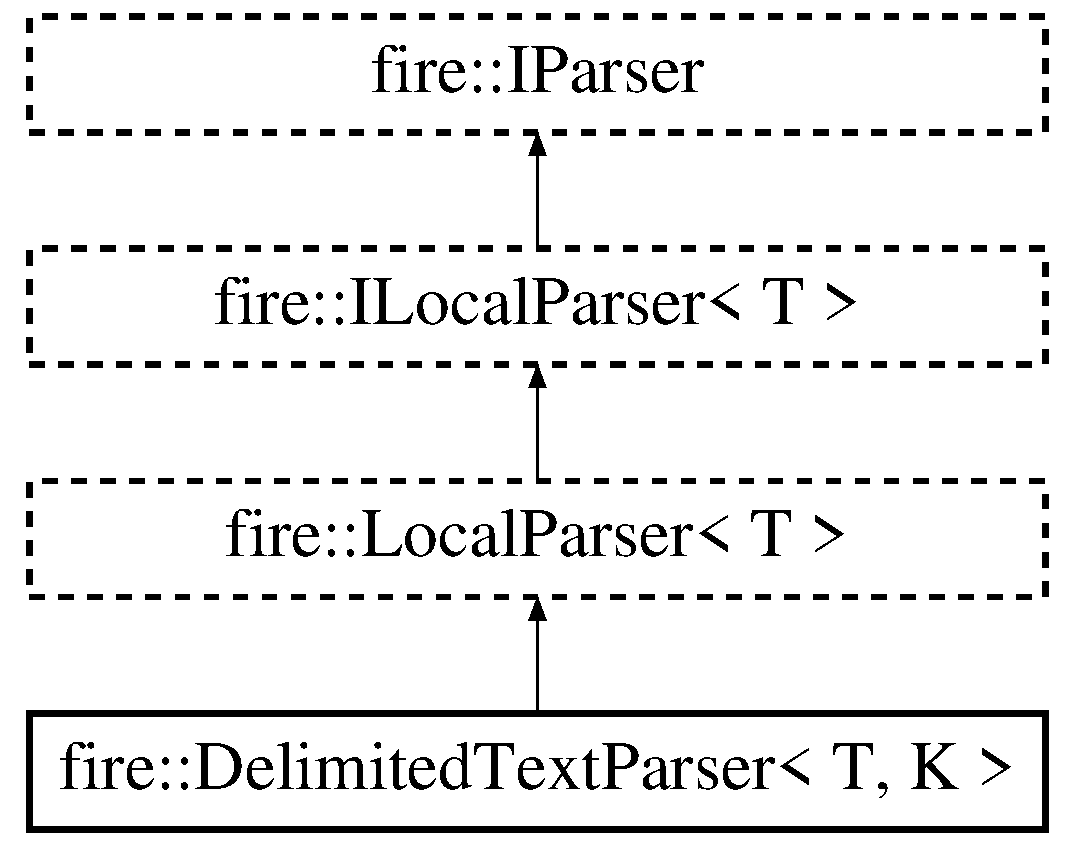
\includegraphics[height=4.000000cm]{a00012}
\end{center}
\end{figure}
\subsection*{Public Member Functions}
\begin{DoxyCompactItemize}
\item 
\hypertarget{a00012_aa1f041ebbf0bf72145e8bd20bf95f3f4}{}{\bfseries Delimited\+Text\+Parser} (string delim, string comment)\label{a00012_aa1f041ebbf0bf72145e8bd20bf95f3f4}

\item 
virtual void \hyperlink{a00012_a686df5548771cae833d5e721442a821a}{parse} ()
\item 
{\footnotesize template$<$$>$ }\\void \hyperlink{a00012_a773fa7ed28cb9d8c384ad94bd81fc93f}{parse} ()
\end{DoxyCompactItemize}
\subsection*{Protected Attributes}
\begin{DoxyCompactItemize}
\item 
string \hyperlink{a00012_ac817fc333b53611a41f446977461bdbf}{delimiter}
\item 
string \hyperlink{a00012_acdd7b27b8109ed41e7d9bc5e6de72e93}{comment\+Char}
\end{DoxyCompactItemize}


\subsection{Detailed Description}
\subsubsection*{template$<$typename T, typename K$>$class fire\+::\+Delimited\+Text\+Parser$<$ T, K $>$}

This class implements \hyperlink{a00019}{I\+Local\+Parser} to provide a local, file-\/based, serially executed delimited text parser.

\hyperlink{a00019_a091d5cf56bf8f407854ef87f460b2958}{is\+File()} will return true if set\+Source(string) is used is\+Stream() will return true if set\+Source(istream) is used \hyperlink{a00019_a770acae6e216de3a9c7140a12de25d58}{is\+Local()} always returns true. \hyperlink{a00019_ad46898c516adcce38acbb4800dc9777b}{is\+Parallel()} always returns false.

Because delimited text is most often primitives, this class requires two template arguments. The first argument T is how the data should be returned and the second argument K is the root type of the delimited text, most likely a primitive. This would look something like


\begin{DoxyCode}
DelimitedTextParser<vector<vector<double>>,\textcolor{keywordtype}{double}>
\end{DoxyCode}


for a dense body of text like in a standard C\+S\+V file or D\+A\+T file where each column is composed of dense primitives.

The source may either be a file on the local filesystem or an input stream.

This is an extension of the parser interface that focuses on parsing delimited text. Delimited text is text with entries that are separated by a common pattern, such as a common or space.

The Comma-\/\+Separated Variables format is a delimited text format of the form

v1, v2, v3, v4

where each comma is the delimiter between the text values v1 through v4. A line of text with only spaces is also a delimited text format\+:

v1 v2 v3 v4

Delimited text parsers may assume that lines such as those above are terminated by ~\newline
. Like most other text formats, delimited text files may contain comments, which may be skipped by I\+Delimited\+Text\+Parsers. The characters that denote comments -\/ very commonly a \char`\"{}\#\char`\"{} or \char`\"{}//\char`\"{} -\/ may be passed to the constructor. 

\subsection{Member Function Documentation}
\hypertarget{a00012_a686df5548771cae833d5e721442a821a}{}\index{fire\+::\+Delimited\+Text\+Parser@{fire\+::\+Delimited\+Text\+Parser}!parse@{parse}}
\index{parse@{parse}!fire\+::\+Delimited\+Text\+Parser@{fire\+::\+Delimited\+Text\+Parser}}
\subsubsection[{parse()}]{\setlength{\rightskip}{0pt plus 5cm}template$<$typename T , typename K $>$ virtual void {\bf fire\+::\+Delimited\+Text\+Parser}$<$ T, K $>$\+::parse (
\begin{DoxyParamCaption}
{}
\end{DoxyParamCaption}
)\hspace{0.3cm}{\ttfamily [inline]}, {\ttfamily [virtual]}}\label{a00012_a686df5548771cae833d5e721442a821a}
This operation directs the parser to parse its source. 

Reimplemented from \hyperlink{a00029_abd8929aea06c2dda40256d2e58236650}{fire\+::\+Local\+Parser$<$ T $>$}.

\hypertarget{a00012_a773fa7ed28cb9d8c384ad94bd81fc93f}{}\index{fire\+::\+Delimited\+Text\+Parser@{fire\+::\+Delimited\+Text\+Parser}!parse@{parse}}
\index{parse@{parse}!fire\+::\+Delimited\+Text\+Parser@{fire\+::\+Delimited\+Text\+Parser}}
\subsubsection[{parse()}]{\setlength{\rightskip}{0pt plus 5cm}template$<$$>$ void {\bf fire\+::\+Delimited\+Text\+Parser}$<$ vector$<$ vector$<$ double $>$ $>$, double $>$\+::parse (
\begin{DoxyParamCaption}
{}
\end{DoxyParamCaption}
)\hspace{0.3cm}{\ttfamily [virtual]}}\label{a00012_a773fa7ed28cb9d8c384ad94bd81fc93f}
This specialization is for dense data of primitive type double. 

Reimplemented from \hyperlink{a00029_abd8929aea06c2dda40256d2e58236650}{fire\+::\+Local\+Parser$<$ T $>$}.



\subsection{Member Data Documentation}
\hypertarget{a00012_acdd7b27b8109ed41e7d9bc5e6de72e93}{}\index{fire\+::\+Delimited\+Text\+Parser@{fire\+::\+Delimited\+Text\+Parser}!comment\+Char@{comment\+Char}}
\index{comment\+Char@{comment\+Char}!fire\+::\+Delimited\+Text\+Parser@{fire\+::\+Delimited\+Text\+Parser}}
\subsubsection[{comment\+Char}]{\setlength{\rightskip}{0pt plus 5cm}template$<$typename T , typename K $>$ string {\bf fire\+::\+Delimited\+Text\+Parser}$<$ T, K $>$\+::comment\+Char\hspace{0.3cm}{\ttfamily [protected]}}\label{a00012_acdd7b27b8109ed41e7d9bc5e6de72e93}
The character that represents a comment and should be skipped. \hypertarget{a00012_ac817fc333b53611a41f446977461bdbf}{}\index{fire\+::\+Delimited\+Text\+Parser@{fire\+::\+Delimited\+Text\+Parser}!delimiter@{delimiter}}
\index{delimiter@{delimiter}!fire\+::\+Delimited\+Text\+Parser@{fire\+::\+Delimited\+Text\+Parser}}
\subsubsection[{delimiter}]{\setlength{\rightskip}{0pt plus 5cm}template$<$typename T , typename K $>$ string {\bf fire\+::\+Delimited\+Text\+Parser}$<$ T, K $>$\+::delimiter\hspace{0.3cm}{\ttfamily [protected]}}\label{a00012_ac817fc333b53611a41f446977461bdbf}
The delimiter used when parsing the file. 

The documentation for this class was generated from the following file\+:\begin{DoxyCompactItemize}
\item 
Delimited\+Text\+Parser.\+h\end{DoxyCompactItemize}

\hypertarget{a00013}{}\section{fire\+:\+:I\+N\+I\+Property\+Parser Class Reference}
\label{a00013}\index{fire\+::\+I\+N\+I\+Property\+Parser@{fire\+::\+I\+N\+I\+Property\+Parser}}


{\ttfamily \#include $<$I\+N\+I\+Property\+Parser.\+h$>$}

Inheritance diagram for fire\+:\+:I\+N\+I\+Property\+Parser\+:\begin{figure}[H]
\begin{center}
\leavevmode
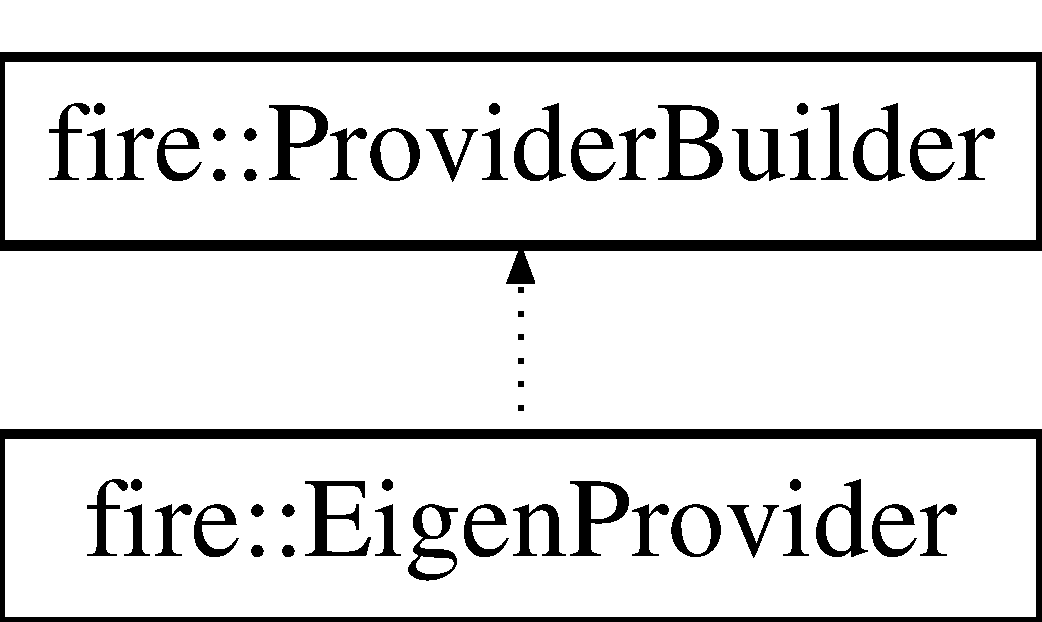
\includegraphics[height=5.000000cm]{a00013}
\end{center}
\end{figure}
\subsection*{Public Member Functions}
\begin{DoxyCompactItemize}
\item 
virtual void \hyperlink{a00013_a06793909bc707a69d0c5772b14bc946d}{set\+Source} (const std\+::string \&source)
\item 
virtual const std\+::string \& \hyperlink{a00013_ad02c9a530f20a706d7bb2554813e8d3a}{get\+Source} ()
\item 
virtual void \hyperlink{a00013_a31b6bad01e65ed4bb5f1ba297616c641}{parse} ()
\item 
virtual const std\+::vector$<$ std\+::string $>$ \& \hyperlink{a00013_aed0f1f47111794659564dcddb4d25bc6}{get\+Property\+Block\+Names} ()
\item 
virtual const std\+::map$<$ std\+::string, std\+::string $>$ \& \hyperlink{a00013_a3591312590a66659ebd377cdde9ab9ad}{get\+Property\+Block} (const std\+::string \&name)
\end{DoxyCompactItemize}
\subsection*{Additional Inherited Members}


\subsection{Detailed Description}
This class implements \hyperlink{a00015}{I\+Property\+Parser} to provide a local, file-\/based, serially executed I\+NI parser.

\hyperlink{a00012_a091d5cf56bf8f407854ef87f460b2958}{is\+File()} always returns true. \hyperlink{a00012_a770acae6e216de3a9c7140a12de25d58}{is\+Local()} always returns true. \hyperlink{a00012_ad46898c516adcce38acbb4800dc9777b}{is\+Parallel()} always returns false.

This implementation is backed by Simple\+I\+NI, one of Fire\textquotesingle{}s dependencies, so it supports whatever Simple\+I\+NI supports.

The source must be a file on the local filesystem. 

\subsection{Member Function Documentation}
\index{fire\+::\+I\+N\+I\+Property\+Parser@{fire\+::\+I\+N\+I\+Property\+Parser}!get\+Property\+Block@{get\+Property\+Block}}
\index{get\+Property\+Block@{get\+Property\+Block}!fire\+::\+I\+N\+I\+Property\+Parser@{fire\+::\+I\+N\+I\+Property\+Parser}}
\subsubsection[{\texorpdfstring{get\+Property\+Block(const std\+::string \&name)}{getPropertyBlock(const std::string \&name)}}]{\setlength{\rightskip}{0pt plus 5cm}virtual const std\+::map$<$std\+::string, std\+::string$>$\& fire\+::\+I\+N\+I\+Property\+Parser\+::get\+Property\+Block (
\begin{DoxyParamCaption}
\item[{const std\+::string \&}]{name}
\end{DoxyParamCaption}
)\hspace{0.3cm}{\ttfamily [inline]}, {\ttfamily [virtual]}}\hypertarget{a00013_a3591312590a66659ebd377cdde9ab9ad}{}\label{a00013_a3591312590a66659ebd377cdde9ab9ad}
This operation returns the property block with the given name. 
\begin{DoxyParams}{Parameters}
{\em name} & the block name \\
\hline
\end{DoxyParams}
\begin{DoxyReturn}{Returns}
the property block with the given name 
\end{DoxyReturn}


Implements \hyperlink{a00015_a34201371cb36dd09e96a66242ececb86}{fire\+::\+I\+Property\+Parser}.

\index{fire\+::\+I\+N\+I\+Property\+Parser@{fire\+::\+I\+N\+I\+Property\+Parser}!get\+Property\+Block\+Names@{get\+Property\+Block\+Names}}
\index{get\+Property\+Block\+Names@{get\+Property\+Block\+Names}!fire\+::\+I\+N\+I\+Property\+Parser@{fire\+::\+I\+N\+I\+Property\+Parser}}
\subsubsection[{\texorpdfstring{get\+Property\+Block\+Names()}{getPropertyBlockNames()}}]{\setlength{\rightskip}{0pt plus 5cm}virtual const std\+::vector$<$std\+::string$>$\& fire\+::\+I\+N\+I\+Property\+Parser\+::get\+Property\+Block\+Names (
\begin{DoxyParamCaption}
{}
\end{DoxyParamCaption}
)\hspace{0.3cm}{\ttfamily [inline]}, {\ttfamily [virtual]}}\hypertarget{a00013_aed0f1f47111794659564dcddb4d25bc6}{}\label{a00013_aed0f1f47111794659564dcddb4d25bc6}
This operation returns the names of the property blocks parsed from the source. \begin{DoxyReturn}{Returns}
the block names 
\end{DoxyReturn}


Implements \hyperlink{a00015_a34602687f9d1affac7bd842102d4a6aa}{fire\+::\+I\+Property\+Parser}.

\index{fire\+::\+I\+N\+I\+Property\+Parser@{fire\+::\+I\+N\+I\+Property\+Parser}!get\+Source@{get\+Source}}
\index{get\+Source@{get\+Source}!fire\+::\+I\+N\+I\+Property\+Parser@{fire\+::\+I\+N\+I\+Property\+Parser}}
\subsubsection[{\texorpdfstring{get\+Source()}{getSource()}}]{\setlength{\rightskip}{0pt plus 5cm}virtual const std\+::string\& fire\+::\+I\+N\+I\+Property\+Parser\+::get\+Source (
\begin{DoxyParamCaption}
{}
\end{DoxyParamCaption}
)\hspace{0.3cm}{\ttfamily [inline]}, {\ttfamily [virtual]}}\hypertarget{a00013_ad02c9a530f20a706d7bb2554813e8d3a}{}\label{a00013_ad02c9a530f20a706d7bb2554813e8d3a}
This operation gets the data source for the parser. \begin{DoxyReturn}{Returns}
the name of the source 
\end{DoxyReturn}


Reimplemented from \hyperlink{a00019_aedb7fe10911182525a719963b9b56726}{fire\+::\+Local\+Parser$<$ std\+::string $>$}.

\index{fire\+::\+I\+N\+I\+Property\+Parser@{fire\+::\+I\+N\+I\+Property\+Parser}!parse@{parse}}
\index{parse@{parse}!fire\+::\+I\+N\+I\+Property\+Parser@{fire\+::\+I\+N\+I\+Property\+Parser}}
\subsubsection[{\texorpdfstring{parse()}{parse()}}]{\setlength{\rightskip}{0pt plus 5cm}virtual void fire\+::\+I\+N\+I\+Property\+Parser\+::parse (
\begin{DoxyParamCaption}
{}
\end{DoxyParamCaption}
)\hspace{0.3cm}{\ttfamily [inline]}, {\ttfamily [virtual]}}\hypertarget{a00013_a31b6bad01e65ed4bb5f1ba297616c641}{}\label{a00013_a31b6bad01e65ed4bb5f1ba297616c641}
This operation directs the parser to parse its source. 

Reimplemented from \hyperlink{a00019_abd8929aea06c2dda40256d2e58236650}{fire\+::\+Local\+Parser$<$ std\+::string $>$}.

\index{fire\+::\+I\+N\+I\+Property\+Parser@{fire\+::\+I\+N\+I\+Property\+Parser}!set\+Source@{set\+Source}}
\index{set\+Source@{set\+Source}!fire\+::\+I\+N\+I\+Property\+Parser@{fire\+::\+I\+N\+I\+Property\+Parser}}
\subsubsection[{\texorpdfstring{set\+Source(const std\+::string \&source)}{setSource(const std::string \&source)}}]{\setlength{\rightskip}{0pt plus 5cm}virtual void fire\+::\+I\+N\+I\+Property\+Parser\+::set\+Source (
\begin{DoxyParamCaption}
\item[{const std\+::string \&}]{source}
\end{DoxyParamCaption}
)\hspace{0.3cm}{\ttfamily [inline]}, {\ttfamily [virtual]}}\hypertarget{a00013_a06793909bc707a69d0c5772b14bc946d}{}\label{a00013_a06793909bc707a69d0c5772b14bc946d}
This operation sets the data source for the parser. 
\begin{DoxyParams}{Parameters}
{\em source} & the name of the source that the parser should parse. \\
\hline
\end{DoxyParams}


Reimplemented from \hyperlink{a00019_afcaec6429fdd6e5d53642a32c001ff73}{fire\+::\+Local\+Parser$<$ std\+::string $>$}.



The documentation for this class was generated from the following file\+:\begin{DoxyCompactItemize}
\item 
I\+N\+I\+Property\+Parser.\+h\end{DoxyCompactItemize}

\hypertarget{a00014}{}\section{fire\+:\+:Eigen\+Tensor\+Provider$<$ Rank, Scalar $>$ Class Template Reference}
\label{a00014}\index{fire\+::\+Eigen\+Tensor\+Provider$<$ Rank, Scalar $>$@{fire\+::\+Eigen\+Tensor\+Provider$<$ Rank, Scalar $>$}}


{\ttfamily \#include $<$Eigen\+Tensor\+Provider.\+hpp$>$}

Inheritance diagram for fire\+:\+:Eigen\+Tensor\+Provider$<$ Rank, Scalar $>$\+:\begin{figure}[H]
\begin{center}
\leavevmode
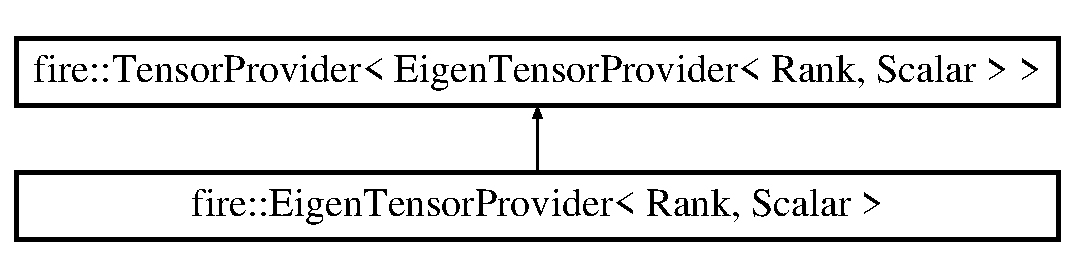
\includegraphics[height=2.000000cm]{a00014}
\end{center}
\end{figure}
\subsection*{Public Member Functions}
\begin{DoxyCompactItemize}
\item 
\hyperlink{a00014_a666937cbdec96978bdd47132a95ab9e6}{Eigen\+Tensor\+Provider} ()
\item 
{\footnotesize template$<$typename... Dimensions$>$ }\\void \hyperlink{a00014_a2d624402c063c0398f018417aae2fe28}{initialize\+Tensor\+Backend} (int first\+Dim, Dimensions...\+other\+Dims)
\item 
void \hyperlink{a00014_a135f00852433ce76d65d8e97e742b60f}{initialize\+Tensor\+Backend\+With\+Reference} (\hyperlink{a00103_a744d7805ef98562de55f32012ab11cfb}{Tensor\+Reference} \&reference)
\item 
{\footnotesize template$<$typename... Indices$>$ }\\double \& \hyperlink{a00014_af546ed4af5f2085c29fc499303bd681a}{tensor\+Coefficient} (Indices...\+indices)
\item 
bool \hyperlink{a00014_af0f8d3e7d83dbd3271ace3f1380d8c7f}{check\+Equality} (\hyperlink{a00103_a744d7805ef98562de55f32012ab11cfb}{Tensor\+Reference} \&other)
\item 
{\footnotesize template$<$typename Other\+Derived , typename Contraction\+Dims $>$ }\\\hyperlink{a00103_a744d7805ef98562de55f32012ab11cfb}{Tensor\+Reference} \hyperlink{a00014_a399a801dc4b785e93893030b84d6b3e2}{execute\+Contraction} (Other\+Derived \&t2, Contraction\+Dims \&c\+Indices)
\item 
Scalar $\ast$ \hyperlink{a00014_aff5626be9e55f593f0a6b71174ecbd8a}{data} ()
\item 
\hyperlink{a00103_a744d7805ef98562de55f32012ab11cfb}{Tensor\+Reference} \hyperlink{a00014_a4bda8a253c803e650987c20628c81c65}{add} (\hyperlink{a00103_a744d7805ef98562de55f32012ab11cfb}{Tensor\+Reference} \&other)
\item 
{\footnotesize template$<$typename Init\+List $>$ }\\void \hyperlink{a00014_a3d02dbf7e2d255a1378084aa6459cf25}{set\+Tensor\+Values} (Init\+List \&vals)
\item 
void \hyperlink{a00014_a607ad28d9f0b8b7f639dc1b0693dfd03}{print\+Tensor} (std\+::ostream \&stream)
\item 
void \hyperlink{a00014_a461c3348c66ae011167d8c194c79dce9}{fill\+With\+Random\+Values} ()
\item 
\hyperlink{a00103_a744d7805ef98562de55f32012ab11cfb}{Tensor\+Reference} \hyperlink{a00014_a0c28a71c68f8ba5f07a45421900e8af5}{scalar\+Product} (Scalar \&val)
\item 
{\footnotesize template$<$typename Dim\+Array $>$ }\\\hyperlink{a00103_a744d7805ef98562de55f32012ab11cfb}{Tensor\+Reference} \hyperlink{a00014_adca448f3689d78ea3f4b306904feccb0}{reshape\+Tensor} (Dim\+Array \&array)
\item 
\hypertarget{a00014_a224630f48894240b4e0e0720a505fc1d}{}{\footnotesize template$<$typename Dim\+Array $>$ }\\\hyperlink{a00103_a744d7805ef98562de55f32012ab11cfb}{Tensor\+Reference} {\bfseries shuffle\+Tensor} (Dim\+Array \&array)\label{a00014_a224630f48894240b4e0e0720a505fc1d}

\item 
\hypertarget{a00014_a31efdc5a7e4620e799e5d91ba9d069fd}{}std\+::pair$<$ \hyperlink{a00103_a744d7805ef98562de55f32012ab11cfb}{Tensor\+Reference}, \hyperlink{a00103_a744d7805ef98562de55f32012ab11cfb}{Tensor\+Reference} $>$ {\bfseries compute\+Svd} (\hyperlink{a00103_a744d7805ef98562de55f32012ab11cfb}{Tensor\+Reference} \&ref, double cutoff)\label{a00014_a31efdc5a7e4620e799e5d91ba9d069fd}

\end{DoxyCompactItemize}
\subsection*{Static Public Member Functions}
\begin{DoxyCompactItemize}
\item 
static constexpr int \hyperlink{a00014_a68f0ad7ead91dec2ea56f173981465c8}{get\+Rank} ()
\end{DoxyCompactItemize}
\subsection*{Static Public Attributes}
\begin{DoxyCompactItemize}
\item 
static const int \hyperlink{a00014_ae8f0217985d78dba31d7bdb95ace1e43}{rank} = Rank
\end{DoxyCompactItemize}


\subsection{Detailed Description}
\subsubsection*{template$<$const int Rank, typename Scalar = double$>$class fire\+::\+Eigen\+Tensor\+Provider$<$ Rank, Scalar $>$}

The \hyperlink{a00014}{Eigen\+Tensor\+Provider} is a \hyperlink{a00047}{Tensor\+Provider} that provides tensor data and operations using the Eigen C++ tensor module. 

\subsection{Constructor \& Destructor Documentation}
\hypertarget{a00014_a666937cbdec96978bdd47132a95ab9e6}{}\index{fire\+::\+Eigen\+Tensor\+Provider@{fire\+::\+Eigen\+Tensor\+Provider}!Eigen\+Tensor\+Provider@{Eigen\+Tensor\+Provider}}
\index{Eigen\+Tensor\+Provider@{Eigen\+Tensor\+Provider}!fire\+::\+Eigen\+Tensor\+Provider@{fire\+::\+Eigen\+Tensor\+Provider}}
\subsubsection[{Eigen\+Tensor\+Provider()}]{\setlength{\rightskip}{0pt plus 5cm}template$<$const int Rank, typename Scalar = double$>$ {\bf fire\+::\+Eigen\+Tensor\+Provider}$<$ Rank, Scalar $>$\+::{\bf Eigen\+Tensor\+Provider} (
\begin{DoxyParamCaption}
{}
\end{DoxyParamCaption}
)\hspace{0.3cm}{\ttfamily [inline]}}\label{a00014_a666937cbdec96978bdd47132a95ab9e6}
The Constructor 

\subsection{Member Function Documentation}
\hypertarget{a00014_a4bda8a253c803e650987c20628c81c65}{}\index{fire\+::\+Eigen\+Tensor\+Provider@{fire\+::\+Eigen\+Tensor\+Provider}!add@{add}}
\index{add@{add}!fire\+::\+Eigen\+Tensor\+Provider@{fire\+::\+Eigen\+Tensor\+Provider}}
\subsubsection[{add(\+Tensor\+Reference \&other)}]{\setlength{\rightskip}{0pt plus 5cm}template$<$const int Rank, typename Scalar = double$>$ {\bf Tensor\+Reference} {\bf fire\+::\+Eigen\+Tensor\+Provider}$<$ Rank, Scalar $>$\+::add (
\begin{DoxyParamCaption}
\item[{{\bf Tensor\+Reference} \&}]{other}
\end{DoxyParamCaption}
)\hspace{0.3cm}{\ttfamily [inline]}}\label{a00014_a4bda8a253c803e650987c20628c81c65}
Return a Tensor\+Reference representing the sum of this Eigen \hyperlink{a00046}{Tensor} and an Eigen \hyperlink{a00046}{Tensor} represented by the other Tensor\+Reference.


\begin{DoxyParams}{Parameters}
{\em other} & Tensor\+Reference view of the other \hyperlink{a00046}{Tensor} \\
\hline
\end{DoxyParams}
\begin{DoxyReturn}{Returns}
result A new Tensor\+Reference representing the sum of this and other. 
\end{DoxyReturn}
\hypertarget{a00014_af0f8d3e7d83dbd3271ace3f1380d8c7f}{}\index{fire\+::\+Eigen\+Tensor\+Provider@{fire\+::\+Eigen\+Tensor\+Provider}!check\+Equality@{check\+Equality}}
\index{check\+Equality@{check\+Equality}!fire\+::\+Eigen\+Tensor\+Provider@{fire\+::\+Eigen\+Tensor\+Provider}}
\subsubsection[{check\+Equality(\+Tensor\+Reference \&other)}]{\setlength{\rightskip}{0pt plus 5cm}template$<$const int Rank, typename Scalar = double$>$ bool {\bf fire\+::\+Eigen\+Tensor\+Provider}$<$ Rank, Scalar $>$\+::check\+Equality (
\begin{DoxyParamCaption}
\item[{{\bf Tensor\+Reference} \&}]{other}
\end{DoxyParamCaption}
)\hspace{0.3cm}{\ttfamily [inline]}}\label{a00014_af0f8d3e7d83dbd3271ace3f1380d8c7f}
Return true if the provided Tensor\+Reference as a tensor is equal to this tensor.


\begin{DoxyParams}{Parameters}
{\em other} & Tensor\+Reference view of the other \hyperlink{a00046}{Tensor} \\
\hline
\end{DoxyParams}
\begin{DoxyReturn}{Returns}
equal A boolean indicating if these Tensors are equal 
\end{DoxyReturn}
\hypertarget{a00014_aff5626be9e55f593f0a6b71174ecbd8a}{}\index{fire\+::\+Eigen\+Tensor\+Provider@{fire\+::\+Eigen\+Tensor\+Provider}!data@{data}}
\index{data@{data}!fire\+::\+Eigen\+Tensor\+Provider@{fire\+::\+Eigen\+Tensor\+Provider}}
\subsubsection[{data()}]{\setlength{\rightskip}{0pt plus 5cm}template$<$const int Rank, typename Scalar = double$>$ Scalar$\ast$ {\bf fire\+::\+Eigen\+Tensor\+Provider}$<$ Rank, Scalar $>$\+::data (
\begin{DoxyParamCaption}
{}
\end{DoxyParamCaption}
)\hspace{0.3cm}{\ttfamily [inline]}}\label{a00014_aff5626be9e55f593f0a6b71174ecbd8a}
Return the 1-\/\+D array wrapped by this Eigen \hyperlink{a00046}{Tensor}

\begin{DoxyReturn}{Returns}
data 1-\/\+D array of data representing the tensor in this \hyperlink{a00047}{Tensor\+Provider} 
\end{DoxyReturn}
\hypertarget{a00014_a399a801dc4b785e93893030b84d6b3e2}{}\index{fire\+::\+Eigen\+Tensor\+Provider@{fire\+::\+Eigen\+Tensor\+Provider}!execute\+Contraction@{execute\+Contraction}}
\index{execute\+Contraction@{execute\+Contraction}!fire\+::\+Eigen\+Tensor\+Provider@{fire\+::\+Eigen\+Tensor\+Provider}}
\subsubsection[{execute\+Contraction(\+Other\+Derived \&t2, Contraction\+Dims \&c\+Indices)}]{\setlength{\rightskip}{0pt plus 5cm}template$<$const int Rank, typename Scalar = double$>$ template$<$typename Other\+Derived , typename Contraction\+Dims $>$ {\bf Tensor\+Reference} {\bf fire\+::\+Eigen\+Tensor\+Provider}$<$ Rank, Scalar $>$\+::execute\+Contraction (
\begin{DoxyParamCaption}
\item[{Other\+Derived \&}]{t2, }
\item[{Contraction\+Dims \&}]{c\+Indices}
\end{DoxyParamCaption}
)\hspace{0.3cm}{\ttfamily [inline]}}\label{a00014_a399a801dc4b785e93893030b84d6b3e2}
Compute the tensor contraction of this Eigen \hyperlink{a00046}{Tensor} with the provided Other \hyperlink{a00046}{Tensor}.


\begin{DoxyParams}{Parameters}
{\em t2} & The other \hyperlink{a00046}{Tensor} \\
\hline
{\em indices} & The contraction indices. \\
\hline
\end{DoxyParams}
\begin{DoxyReturn}{Returns}
result The contraction result as a Tensor\+Reference 
\end{DoxyReturn}
\hypertarget{a00014_a461c3348c66ae011167d8c194c79dce9}{}\index{fire\+::\+Eigen\+Tensor\+Provider@{fire\+::\+Eigen\+Tensor\+Provider}!fill\+With\+Random\+Values@{fill\+With\+Random\+Values}}
\index{fill\+With\+Random\+Values@{fill\+With\+Random\+Values}!fire\+::\+Eigen\+Tensor\+Provider@{fire\+::\+Eigen\+Tensor\+Provider}}
\subsubsection[{fill\+With\+Random\+Values()}]{\setlength{\rightskip}{0pt plus 5cm}template$<$const int Rank, typename Scalar = double$>$ void {\bf fire\+::\+Eigen\+Tensor\+Provider}$<$ Rank, Scalar $>$\+::fill\+With\+Random\+Values (
\begin{DoxyParamCaption}
{}
\end{DoxyParamCaption}
)\hspace{0.3cm}{\ttfamily [inline]}}\label{a00014_a461c3348c66ae011167d8c194c79dce9}
Set the Eigen \hyperlink{a00046}{Tensor} values to random values. \hypertarget{a00014_a68f0ad7ead91dec2ea56f173981465c8}{}\index{fire\+::\+Eigen\+Tensor\+Provider@{fire\+::\+Eigen\+Tensor\+Provider}!get\+Rank@{get\+Rank}}
\index{get\+Rank@{get\+Rank}!fire\+::\+Eigen\+Tensor\+Provider@{fire\+::\+Eigen\+Tensor\+Provider}}
\subsubsection[{get\+Rank()}]{\setlength{\rightskip}{0pt plus 5cm}template$<$const int Rank, typename Scalar = double$>$ static constexpr int {\bf fire\+::\+Eigen\+Tensor\+Provider}$<$ Rank, Scalar $>$\+::get\+Rank (
\begin{DoxyParamCaption}
{}
\end{DoxyParamCaption}
)\hspace{0.3cm}{\ttfamily [inline]}, {\ttfamily [static]}}\label{a00014_a68f0ad7ead91dec2ea56f173981465c8}
Return the rank of this Eigen \hyperlink{a00046}{Tensor}

\begin{DoxyReturn}{Returns}
rank The rank of this \hyperlink{a00046}{Tensor} 
\end{DoxyReturn}
\hypertarget{a00014_a2d624402c063c0398f018417aae2fe28}{}\index{fire\+::\+Eigen\+Tensor\+Provider@{fire\+::\+Eigen\+Tensor\+Provider}!initialize\+Tensor\+Backend@{initialize\+Tensor\+Backend}}
\index{initialize\+Tensor\+Backend@{initialize\+Tensor\+Backend}!fire\+::\+Eigen\+Tensor\+Provider@{fire\+::\+Eigen\+Tensor\+Provider}}
\subsubsection[{initialize\+Tensor\+Backend(int first\+Dim, Dimensions...\+other\+Dims)}]{\setlength{\rightskip}{0pt plus 5cm}template$<$const int Rank, typename Scalar = double$>$ template$<$typename... Dimensions$>$ void {\bf fire\+::\+Eigen\+Tensor\+Provider}$<$ Rank, Scalar $>$\+::initialize\+Tensor\+Backend (
\begin{DoxyParamCaption}
\item[{int}]{first\+Dim, }
\item[{Dimensions...}]{other\+Dims}
\end{DoxyParamCaption}
)\hspace{0.3cm}{\ttfamily [inline]}}\label{a00014_a2d624402c063c0398f018417aae2fe28}
Initialize the Eigen \hyperlink{a00046}{Tensor} with all zeros. 
\begin{DoxyParams}{Parameters}
{\em first\+Dim} & \\
\hline
{\em other\+Dims} & \\
\hline
\end{DoxyParams}
\hypertarget{a00014_a135f00852433ce76d65d8e97e742b60f}{}\index{fire\+::\+Eigen\+Tensor\+Provider@{fire\+::\+Eigen\+Tensor\+Provider}!initialize\+Tensor\+Backend\+With\+Reference@{initialize\+Tensor\+Backend\+With\+Reference}}
\index{initialize\+Tensor\+Backend\+With\+Reference@{initialize\+Tensor\+Backend\+With\+Reference}!fire\+::\+Eigen\+Tensor\+Provider@{fire\+::\+Eigen\+Tensor\+Provider}}
\subsubsection[{initialize\+Tensor\+Backend\+With\+Reference(\+Tensor\+Reference \&reference)}]{\setlength{\rightskip}{0pt plus 5cm}template$<$const int Rank, typename Scalar = double$>$ void {\bf fire\+::\+Eigen\+Tensor\+Provider}$<$ Rank, Scalar $>$\+::initialize\+Tensor\+Backend\+With\+Reference (
\begin{DoxyParamCaption}
\item[{{\bf Tensor\+Reference} \&}]{reference}
\end{DoxyParamCaption}
)\hspace{0.3cm}{\ttfamily [inline]}}\label{a00014_a135f00852433ce76d65d8e97e742b60f}
Initialize the Eigen \hyperlink{a00046}{Tensor} from an existing Tensor\+Reference 
\begin{DoxyParams}{Parameters}
{\em reference} & \\
\hline
\end{DoxyParams}
\hypertarget{a00014_a607ad28d9f0b8b7f639dc1b0693dfd03}{}\index{fire\+::\+Eigen\+Tensor\+Provider@{fire\+::\+Eigen\+Tensor\+Provider}!print\+Tensor@{print\+Tensor}}
\index{print\+Tensor@{print\+Tensor}!fire\+::\+Eigen\+Tensor\+Provider@{fire\+::\+Eigen\+Tensor\+Provider}}
\subsubsection[{print\+Tensor(std\+::ostream \&stream)}]{\setlength{\rightskip}{0pt plus 5cm}template$<$const int Rank, typename Scalar = double$>$ void {\bf fire\+::\+Eigen\+Tensor\+Provider}$<$ Rank, Scalar $>$\+::print\+Tensor (
\begin{DoxyParamCaption}
\item[{std\+::ostream \&}]{stream}
\end{DoxyParamCaption}
)\hspace{0.3cm}{\ttfamily [inline]}}\label{a00014_a607ad28d9f0b8b7f639dc1b0693dfd03}
Output this Eigen \hyperlink{a00046}{Tensor} to the provided output stream.


\begin{DoxyParams}{Parameters}
{\em output\+Stream} & The output stream to write the tensor to. \\
\hline
\end{DoxyParams}
\hypertarget{a00014_adca448f3689d78ea3f4b306904feccb0}{}\index{fire\+::\+Eigen\+Tensor\+Provider@{fire\+::\+Eigen\+Tensor\+Provider}!reshape\+Tensor@{reshape\+Tensor}}
\index{reshape\+Tensor@{reshape\+Tensor}!fire\+::\+Eigen\+Tensor\+Provider@{fire\+::\+Eigen\+Tensor\+Provider}}
\subsubsection[{reshape\+Tensor(\+Dim\+Array \&array)}]{\setlength{\rightskip}{0pt plus 5cm}template$<$const int Rank, typename Scalar = double$>$ template$<$typename Dim\+Array $>$ {\bf Tensor\+Reference} {\bf fire\+::\+Eigen\+Tensor\+Provider}$<$ Rank, Scalar $>$\+::reshape\+Tensor (
\begin{DoxyParamCaption}
\item[{Dim\+Array \&}]{array}
\end{DoxyParamCaption}
)\hspace{0.3cm}{\ttfamily [inline]}}\label{a00014_adca448f3689d78ea3f4b306904feccb0}
Reshape the Eigen \hyperlink{a00046}{Tensor} with a new array of dimensions


\begin{DoxyParams}{Parameters}
{\em array} & Array of new dimensions for each rank index \\
\hline
\end{DoxyParams}
\begin{DoxyReturn}{Returns}
reshaped\+Tensor A Tensor\+Reference representing new reshaped tensor. 
\end{DoxyReturn}
\hypertarget{a00014_a0c28a71c68f8ba5f07a45421900e8af5}{}\index{fire\+::\+Eigen\+Tensor\+Provider@{fire\+::\+Eigen\+Tensor\+Provider}!scalar\+Product@{scalar\+Product}}
\index{scalar\+Product@{scalar\+Product}!fire\+::\+Eigen\+Tensor\+Provider@{fire\+::\+Eigen\+Tensor\+Provider}}
\subsubsection[{scalar\+Product(\+Scalar \&val)}]{\setlength{\rightskip}{0pt plus 5cm}template$<$const int Rank, typename Scalar = double$>$ {\bf Tensor\+Reference} {\bf fire\+::\+Eigen\+Tensor\+Provider}$<$ Rank, Scalar $>$\+::scalar\+Product (
\begin{DoxyParamCaption}
\item[{Scalar \&}]{val}
\end{DoxyParamCaption}
)\hspace{0.3cm}{\ttfamily [inline]}}\label{a00014_a0c28a71c68f8ba5f07a45421900e8af5}
Multiply all elements of this Eigen \hyperlink{a00046}{Tensor} by the provided Scalar.


\begin{DoxyParams}{Parameters}
{\em val} & Scalar to multiply this tensor by. \\
\hline
\end{DoxyParams}
\begin{DoxyReturn}{Returns}
result A Tensor\+Reference representing the result 
\end{DoxyReturn}
\hypertarget{a00014_a3d02dbf7e2d255a1378084aa6459cf25}{}\index{fire\+::\+Eigen\+Tensor\+Provider@{fire\+::\+Eigen\+Tensor\+Provider}!set\+Tensor\+Values@{set\+Tensor\+Values}}
\index{set\+Tensor\+Values@{set\+Tensor\+Values}!fire\+::\+Eigen\+Tensor\+Provider@{fire\+::\+Eigen\+Tensor\+Provider}}
\subsubsection[{set\+Tensor\+Values(\+Init\+List \&vals)}]{\setlength{\rightskip}{0pt plus 5cm}template$<$const int Rank, typename Scalar = double$>$ template$<$typename Init\+List $>$ void {\bf fire\+::\+Eigen\+Tensor\+Provider}$<$ Rank, Scalar $>$\+::set\+Tensor\+Values (
\begin{DoxyParamCaption}
\item[{Init\+List \&}]{vals}
\end{DoxyParamCaption}
)\hspace{0.3cm}{\ttfamily [inline]}}\label{a00014_a3d02dbf7e2d255a1378084aa6459cf25}
Set the Eigen \hyperlink{a00046}{Tensor} values using nested initializer\+\_\+list


\begin{DoxyParams}{Parameters}
{\em vals} & The values as a nest std\+::initializer\+\_\+lists \\
\hline
\end{DoxyParams}
\hypertarget{a00014_af546ed4af5f2085c29fc499303bd681a}{}\index{fire\+::\+Eigen\+Tensor\+Provider@{fire\+::\+Eigen\+Tensor\+Provider}!tensor\+Coefficient@{tensor\+Coefficient}}
\index{tensor\+Coefficient@{tensor\+Coefficient}!fire\+::\+Eigen\+Tensor\+Provider@{fire\+::\+Eigen\+Tensor\+Provider}}
\subsubsection[{tensor\+Coefficient(\+Indices...\+indices)}]{\setlength{\rightskip}{0pt plus 5cm}template$<$const int Rank, typename Scalar = double$>$ template$<$typename... Indices$>$ double\& {\bf fire\+::\+Eigen\+Tensor\+Provider}$<$ Rank, Scalar $>$\+::tensor\+Coefficient (
\begin{DoxyParamCaption}
\item[{Indices...}]{indices}
\end{DoxyParamCaption}
)\hspace{0.3cm}{\ttfamily [inline]}}\label{a00014_af546ed4af5f2085c29fc499303bd681a}
Return the coefficient at the given tensor indices.


\begin{DoxyParams}{Parameters}
{\em indices} & The indices for the desired value \\
\hline
\end{DoxyParams}
\begin{DoxyReturn}{Returns}
val The value at the indices. 
\end{DoxyReturn}


\subsection{Member Data Documentation}
\hypertarget{a00014_ae8f0217985d78dba31d7bdb95ace1e43}{}\index{fire\+::\+Eigen\+Tensor\+Provider@{fire\+::\+Eigen\+Tensor\+Provider}!rank@{rank}}
\index{rank@{rank}!fire\+::\+Eigen\+Tensor\+Provider@{fire\+::\+Eigen\+Tensor\+Provider}}
\subsubsection[{rank}]{\setlength{\rightskip}{0pt plus 5cm}template$<$const int Rank, typename Scalar = double$>$ const int {\bf fire\+::\+Eigen\+Tensor\+Provider}$<$ Rank, Scalar $>$\+::rank = Rank\hspace{0.3cm}{\ttfamily [static]}}\label{a00014_ae8f0217985d78dba31d7bdb95ace1e43}
Static reference to the rank of the tensor wrapped by this provider 

The documentation for this class was generated from the following file\+:\begin{DoxyCompactItemize}
\item 
Eigen\+Tensor\+Provider.\+hpp\end{DoxyCompactItemize}

\hypertarget{a00015}{}\section{fire\+:\+:I\+Property\+Parser Class Reference}
\label{a00015}\index{fire\+::\+I\+Property\+Parser@{fire\+::\+I\+Property\+Parser}}


{\ttfamily \#include $<$I\+Property\+Parser.\+h$>$}

Inheritance diagram for fire\+:\+:I\+Property\+Parser\+:\begin{figure}[H]
\begin{center}
\leavevmode
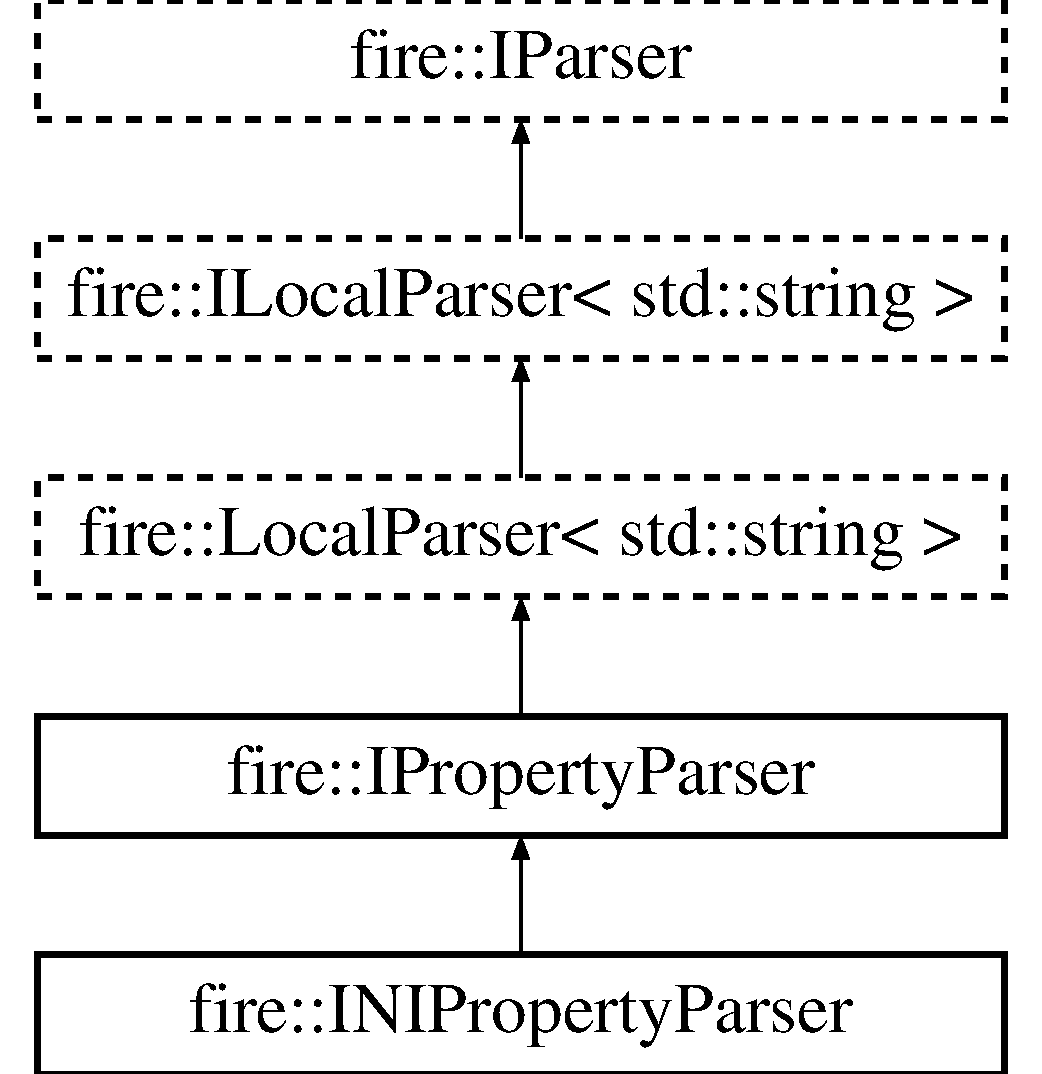
\includegraphics[height=5.000000cm]{a00015}
\end{center}
\end{figure}
\subsection*{Public Member Functions}
\begin{DoxyCompactItemize}
\item 
virtual const std\+::vector$<$ std\+::string $>$ \& \hyperlink{a00015_a34602687f9d1affac7bd842102d4a6aa}{get\+Property\+Block\+Names} ()=0
\item 
virtual const std\+::map$<$ std\+::string, std\+::string $>$ \& \hyperlink{a00015_a34201371cb36dd09e96a66242ececb86}{get\+Property\+Block} (const std\+::string \&name)=0
\end{DoxyCompactItemize}
\subsection*{Additional Inherited Members}


\subsection{Detailed Description}
This is an extension of the parser interface that focuses on parsing a set of properties. Properties are returned in blocks represented by maps.. 

\subsection{Member Function Documentation}
\index{fire\+::\+I\+Property\+Parser@{fire\+::\+I\+Property\+Parser}!get\+Property\+Block@{get\+Property\+Block}}
\index{get\+Property\+Block@{get\+Property\+Block}!fire\+::\+I\+Property\+Parser@{fire\+::\+I\+Property\+Parser}}
\subsubsection[{\texorpdfstring{get\+Property\+Block(const std\+::string \&name)=0}{getPropertyBlock(const std::string \&name)=0}}]{\setlength{\rightskip}{0pt plus 5cm}virtual const std\+::map$<$std\+::string, std\+::string$>$\& fire\+::\+I\+Property\+Parser\+::get\+Property\+Block (
\begin{DoxyParamCaption}
\item[{const std\+::string \&}]{name}
\end{DoxyParamCaption}
)\hspace{0.3cm}{\ttfamily [pure virtual]}}\hypertarget{a00015_a34201371cb36dd09e96a66242ececb86}{}\label{a00015_a34201371cb36dd09e96a66242ececb86}
This operation returns the property block with the given name. 
\begin{DoxyParams}{Parameters}
{\em name} & the block name \\
\hline
\end{DoxyParams}
\begin{DoxyReturn}{Returns}
the property block with the given name 
\end{DoxyReturn}


Implemented in \hyperlink{a00013_a3591312590a66659ebd377cdde9ab9ad}{fire\+::\+I\+N\+I\+Property\+Parser}.

\index{fire\+::\+I\+Property\+Parser@{fire\+::\+I\+Property\+Parser}!get\+Property\+Block\+Names@{get\+Property\+Block\+Names}}
\index{get\+Property\+Block\+Names@{get\+Property\+Block\+Names}!fire\+::\+I\+Property\+Parser@{fire\+::\+I\+Property\+Parser}}
\subsubsection[{\texorpdfstring{get\+Property\+Block\+Names()=0}{getPropertyBlockNames()=0}}]{\setlength{\rightskip}{0pt plus 5cm}virtual const std\+::vector$<$std\+::string$>$\& fire\+::\+I\+Property\+Parser\+::get\+Property\+Block\+Names (
\begin{DoxyParamCaption}
{}
\end{DoxyParamCaption}
)\hspace{0.3cm}{\ttfamily [pure virtual]}}\hypertarget{a00015_a34602687f9d1affac7bd842102d4a6aa}{}\label{a00015_a34602687f9d1affac7bd842102d4a6aa}
This operation returns the names of the property blocks parsed from the source. \begin{DoxyReturn}{Returns}
the block names 
\end{DoxyReturn}


Implemented in \hyperlink{a00013_aed0f1f47111794659564dcddb4d25bc6}{fire\+::\+I\+N\+I\+Property\+Parser}.



The documentation for this class was generated from the following file\+:\begin{DoxyCompactItemize}
\item 
I\+Property\+Parser.\+h\end{DoxyCompactItemize}

\hypertarget{a00016}{}\section{File\+Generator Struct Reference}
\label{a00016}\index{File\+Generator@{File\+Generator}}


The documentation for this struct was generated from the following file\+:\begin{DoxyCompactItemize}
\item 
Delimited\+Text\+Parser\+Test.\+cpp\end{DoxyCompactItemize}

\hypertarget{a00017}{}\section{C\+Simple\+Ini\+Templ$<$ S\+I\+\_\+\+C\+H\+AR, S\+I\+\_\+\+S\+T\+R\+L\+E\+SS, S\+I\+\_\+\+C\+O\+N\+V\+E\+R\+T\+ER $>$\+:\+:Entry\+:\+:Key\+Order Struct Reference}
\label{a00017}\index{C\+Simple\+Ini\+Templ$<$ S\+I\+\_\+\+C\+H\+A\+R, S\+I\+\_\+\+S\+T\+R\+L\+E\+S\+S, S\+I\+\_\+\+C\+O\+N\+V\+E\+R\+T\+E\+R $>$\+::\+Entry\+::\+Key\+Order@{C\+Simple\+Ini\+Templ$<$ S\+I\+\_\+\+C\+H\+A\+R, S\+I\+\_\+\+S\+T\+R\+L\+E\+S\+S, S\+I\+\_\+\+C\+O\+N\+V\+E\+R\+T\+E\+R $>$\+::\+Entry\+::\+Key\+Order}}


{\ttfamily \#include $<$Simple\+Ini.\+h$>$}

Inheritance diagram for C\+Simple\+Ini\+Templ$<$ S\+I\+\_\+\+C\+H\+AR, S\+I\+\_\+\+S\+T\+R\+L\+E\+SS, S\+I\+\_\+\+C\+O\+N\+V\+E\+R\+T\+ER $>$\+:\+:Entry\+:\+:Key\+Order\+:\begin{figure}[H]
\begin{center}
\leavevmode
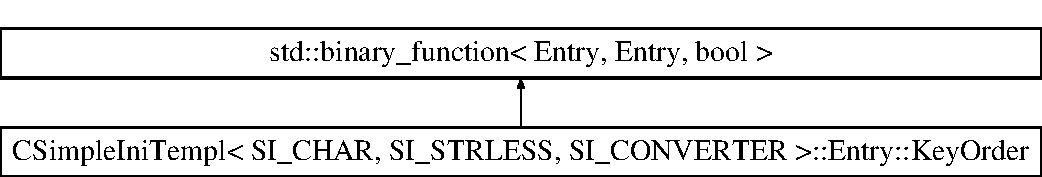
\includegraphics[height=2.000000cm]{a00017}
\end{center}
\end{figure}
\subsection*{Public Member Functions}
\begin{DoxyCompactItemize}
\item 
bool {\bfseries operator()} (const \hyperlink{a00009}{Entry} \&lhs, const \hyperlink{a00009}{Entry} \&rhs) const \hypertarget{a00017_a4cfcbc71e83cc369f55643c715609176}{}\label{a00017_a4cfcbc71e83cc369f55643c715609176}

\end{DoxyCompactItemize}


\subsection{Detailed Description}
\subsubsection*{template$<$class S\+I\+\_\+\+C\+H\+AR, class S\+I\+\_\+\+S\+T\+R\+L\+E\+SS, class S\+I\+\_\+\+C\+O\+N\+V\+E\+R\+T\+ER$>$\\*
struct C\+Simple\+Ini\+Templ$<$ S\+I\+\_\+\+C\+H\+A\+R, S\+I\+\_\+\+S\+T\+R\+L\+E\+S\+S, S\+I\+\_\+\+C\+O\+N\+V\+E\+R\+T\+E\+R $>$\+::\+Entry\+::\+Key\+Order}

Strict less ordering by name of key only 

The documentation for this struct was generated from the following file\+:\begin{DoxyCompactItemize}
\item 
Simple\+Ini.\+h\end{DoxyCompactItemize}

\hypertarget{a00018}{}\section{C\+Simple\+Ini\+Templ$<$ S\+I\+\_\+\+C\+H\+AR, S\+I\+\_\+\+S\+T\+R\+L\+E\+SS, S\+I\+\_\+\+C\+O\+N\+V\+E\+R\+T\+ER $>$\+:\+:Entry\+:\+:Load\+Order Struct Reference}
\label{a00018}\index{C\+Simple\+Ini\+Templ$<$ S\+I\+\_\+\+C\+H\+A\+R, S\+I\+\_\+\+S\+T\+R\+L\+E\+S\+S, S\+I\+\_\+\+C\+O\+N\+V\+E\+R\+T\+E\+R $>$\+::\+Entry\+::\+Load\+Order@{C\+Simple\+Ini\+Templ$<$ S\+I\+\_\+\+C\+H\+A\+R, S\+I\+\_\+\+S\+T\+R\+L\+E\+S\+S, S\+I\+\_\+\+C\+O\+N\+V\+E\+R\+T\+E\+R $>$\+::\+Entry\+::\+Load\+Order}}


{\ttfamily \#include $<$Simple\+Ini.\+h$>$}

Inheritance diagram for C\+Simple\+Ini\+Templ$<$ S\+I\+\_\+\+C\+H\+AR, S\+I\+\_\+\+S\+T\+R\+L\+E\+SS, S\+I\+\_\+\+C\+O\+N\+V\+E\+R\+T\+ER $>$\+:\+:Entry\+:\+:Load\+Order\+:\begin{figure}[H]
\begin{center}
\leavevmode
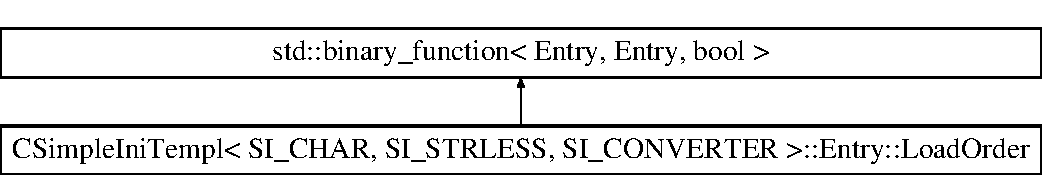
\includegraphics[height=2.000000cm]{a00018}
\end{center}
\end{figure}
\subsection*{Public Member Functions}
\begin{DoxyCompactItemize}
\item 
bool {\bfseries operator()} (const \hyperlink{a00009}{Entry} \&lhs, const \hyperlink{a00009}{Entry} \&rhs) const \hypertarget{a00018_ac92e1aa48e5c9aafe994aab65aff4a48}{}\label{a00018_ac92e1aa48e5c9aafe994aab65aff4a48}

\end{DoxyCompactItemize}


\subsection{Detailed Description}
\subsubsection*{template$<$class S\+I\+\_\+\+C\+H\+AR, class S\+I\+\_\+\+S\+T\+R\+L\+E\+SS, class S\+I\+\_\+\+C\+O\+N\+V\+E\+R\+T\+ER$>$\\*
struct C\+Simple\+Ini\+Templ$<$ S\+I\+\_\+\+C\+H\+A\+R, S\+I\+\_\+\+S\+T\+R\+L\+E\+S\+S, S\+I\+\_\+\+C\+O\+N\+V\+E\+R\+T\+E\+R $>$\+::\+Entry\+::\+Load\+Order}

Strict less ordering by order, and then name of key 

The documentation for this struct was generated from the following file\+:\begin{DoxyCompactItemize}
\item 
Simple\+Ini.\+h\end{DoxyCompactItemize}

\hypertarget{a00019}{}\section{fire\+:\+:I\+Local\+Parser$<$ T $>$ Class Template Reference}
\label{a00019}\index{fire\+::\+I\+Local\+Parser$<$ T $>$@{fire\+::\+I\+Local\+Parser$<$ T $>$}}


{\ttfamily \#include $<$I\+Local\+Parser.\+h$>$}

Inheritance diagram for fire\+:\+:I\+Local\+Parser$<$ T $>$\+:\begin{figure}[H]
\begin{center}
\leavevmode
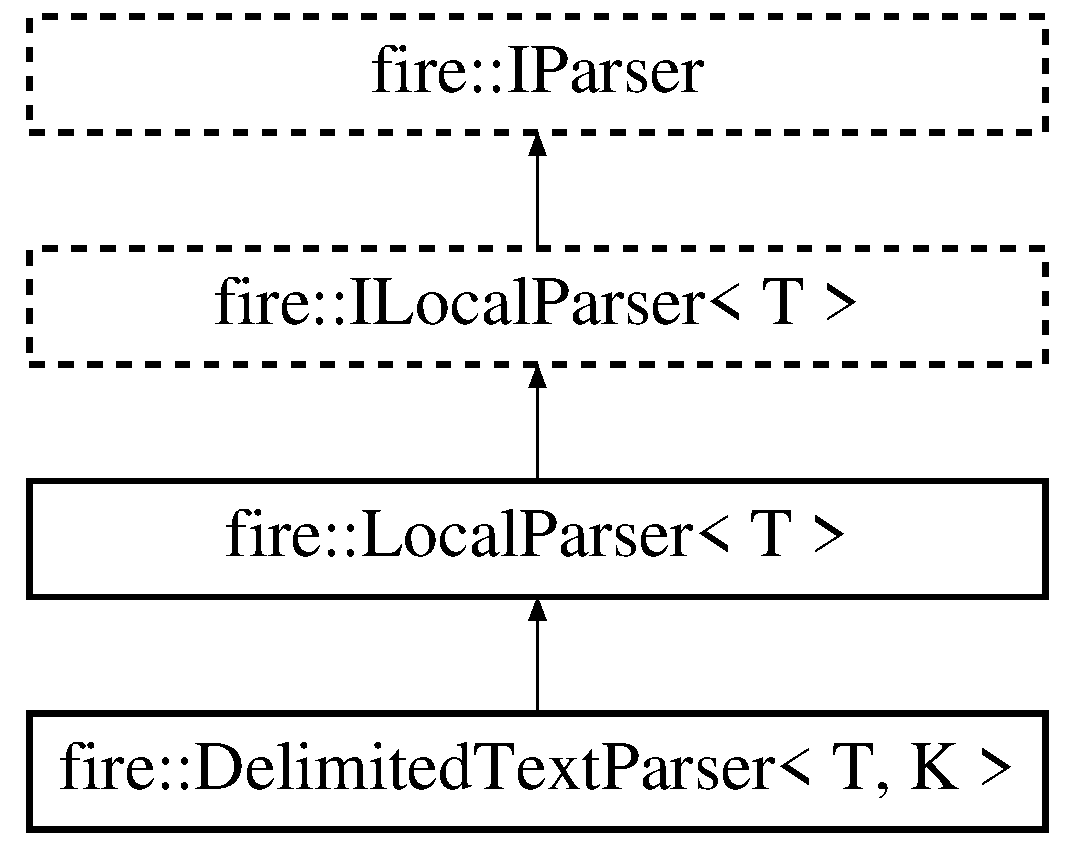
\includegraphics[height=4.000000cm]{a00019}
\end{center}
\end{figure}
\subsection*{Public Member Functions}
\begin{DoxyCompactItemize}
\item 
virtual bool \hyperlink{a00019_a091d5cf56bf8f407854ef87f460b2958}{is\+File} ()
\item 
virtual bool \hyperlink{a00019_a770acae6e216de3a9c7140a12de25d58}{is\+Local} ()
\item 
virtual bool \hyperlink{a00019_ad46898c516adcce38acbb4800dc9777b}{is\+Parallel} ()
\item 
virtual std\+::shared\+\_\+ptr$<$ T $>$ \hyperlink{a00019_a0fc1446d106f0ab8daf8744a4bd29a65}{get\+Data} ()=0
\end{DoxyCompactItemize}
\subsection*{Protected Attributes}
\begin{DoxyCompactItemize}
\item 
bool \hyperlink{a00019_a39adf288ae0bc79cf39fd6e4638858cf}{is\+A\+File} = true
\end{DoxyCompactItemize}


\subsection{Detailed Description}
\subsubsection*{template$<$typename T$>$class fire\+::\+I\+Local\+Parser$<$ T $>$}

This is a sub-\/interface of \hyperlink{a00024}{I\+Parser} that represents a parser for a local, serially executed parser.

\hyperlink{a00019_a770acae6e216de3a9c7140a12de25d58}{is\+Local()} always returns true. \hyperlink{a00019_ad46898c516adcce38acbb4800dc9777b}{is\+Parallel()} always returns false.

Implementations should set is\+File in their set\+Source(std\+::string) if their source is a file. Subclasses must always be sure that they implement \hyperlink{a00024_af36ac6eedd8c27d2f418869193d7d03c}{parse()} and \hyperlink{a00024_a0dbeff2b9bd8dbfb2aad7a424eef87d1}{set\+Source()} because default implementations are not provided.

The \hyperlink{a00019_a0fc1446d106f0ab8daf8744a4bd29a65}{get\+Data()} operation always returns a shared\+\_\+ptr instead of a raw type (copy) or raw pointer to efficiently share the dynamically allocated data. 

\subsection{Member Function Documentation}
\hypertarget{a00019_a0fc1446d106f0ab8daf8744a4bd29a65}{}\index{fire\+::\+I\+Local\+Parser@{fire\+::\+I\+Local\+Parser}!get\+Data@{get\+Data}}
\index{get\+Data@{get\+Data}!fire\+::\+I\+Local\+Parser@{fire\+::\+I\+Local\+Parser}}
\subsubsection[{get\+Data()=0}]{\setlength{\rightskip}{0pt plus 5cm}template$<$typename T$>$ virtual std\+::shared\+\_\+ptr$<$T$>$ {\bf fire\+::\+I\+Local\+Parser}$<$ T $>$\+::get\+Data (
\begin{DoxyParamCaption}
{}
\end{DoxyParamCaption}
)\hspace{0.3cm}{\ttfamily [pure virtual]}}\label{a00019_a0fc1446d106f0ab8daf8744a4bd29a65}
This operation returns a shared pointer to an instance of type T. \begin{DoxyReturn}{Returns}
a shared pointer holding an instance of type T that was parsed from the file. 
\end{DoxyReturn}


Implemented in \hyperlink{a00029_ab9016cca8e5dca516bb57c6a8e76607a}{fire\+::\+Local\+Parser$<$ T $>$}, and \hyperlink{a00029_ab9016cca8e5dca516bb57c6a8e76607a}{fire\+::\+Local\+Parser$<$ std\+::string $>$}.

\hypertarget{a00019_a091d5cf56bf8f407854ef87f460b2958}{}\index{fire\+::\+I\+Local\+Parser@{fire\+::\+I\+Local\+Parser}!is\+File@{is\+File}}
\index{is\+File@{is\+File}!fire\+::\+I\+Local\+Parser@{fire\+::\+I\+Local\+Parser}}
\subsubsection[{is\+File()}]{\setlength{\rightskip}{0pt plus 5cm}template$<$typename T$>$ virtual bool {\bf fire\+::\+I\+Local\+Parser}$<$ T $>$\+::is\+File (
\begin{DoxyParamCaption}
{}
\end{DoxyParamCaption}
)\hspace{0.3cm}{\ttfamily [inline]}, {\ttfamily [virtual]}}\label{a00019_a091d5cf56bf8f407854ef87f460b2958}
This operation indicates whether or not the parser\textquotesingle{}s source is a file. \begin{DoxyReturn}{Returns}
true if this parser is working with a file, false otherwise. 
\end{DoxyReturn}


Implements \hyperlink{a00024_a616c42c85d781c916e97f0ad8f1e9010}{fire\+::\+I\+Parser}.

\hypertarget{a00019_a770acae6e216de3a9c7140a12de25d58}{}\index{fire\+::\+I\+Local\+Parser@{fire\+::\+I\+Local\+Parser}!is\+Local@{is\+Local}}
\index{is\+Local@{is\+Local}!fire\+::\+I\+Local\+Parser@{fire\+::\+I\+Local\+Parser}}
\subsubsection[{is\+Local()}]{\setlength{\rightskip}{0pt plus 5cm}template$<$typename T$>$ virtual bool {\bf fire\+::\+I\+Local\+Parser}$<$ T $>$\+::is\+Local (
\begin{DoxyParamCaption}
{}
\end{DoxyParamCaption}
)\hspace{0.3cm}{\ttfamily [inline]}, {\ttfamily [virtual]}}\label{a00019_a770acae6e216de3a9c7140a12de25d58}
This operation indicates whether or not the parser is using a local source. \begin{DoxyReturn}{Returns}
true if this parser is working with a local source, false otherwise. 
\end{DoxyReturn}


Implements \hyperlink{a00024_a97b9e58493b3cadbc63e670b0b0e759f}{fire\+::\+I\+Parser}.

\hypertarget{a00019_ad46898c516adcce38acbb4800dc9777b}{}\index{fire\+::\+I\+Local\+Parser@{fire\+::\+I\+Local\+Parser}!is\+Parallel@{is\+Parallel}}
\index{is\+Parallel@{is\+Parallel}!fire\+::\+I\+Local\+Parser@{fire\+::\+I\+Local\+Parser}}
\subsubsection[{is\+Parallel()}]{\setlength{\rightskip}{0pt plus 5cm}template$<$typename T$>$ virtual bool {\bf fire\+::\+I\+Local\+Parser}$<$ T $>$\+::is\+Parallel (
\begin{DoxyParamCaption}
{}
\end{DoxyParamCaption}
)\hspace{0.3cm}{\ttfamily [inline]}, {\ttfamily [virtual]}}\label{a00019_ad46898c516adcce38acbb4800dc9777b}
This operation indicates whether or not the parser reads in parallel. \begin{DoxyReturn}{Returns}
true if this parser reads in parallel, false otherwise. 
\end{DoxyReturn}


Implements \hyperlink{a00024_a83d2882a466d694fb0aea3d846bcbed4}{fire\+::\+I\+Parser}.



\subsection{Member Data Documentation}
\hypertarget{a00019_a39adf288ae0bc79cf39fd6e4638858cf}{}\index{fire\+::\+I\+Local\+Parser@{fire\+::\+I\+Local\+Parser}!is\+A\+File@{is\+A\+File}}
\index{is\+A\+File@{is\+A\+File}!fire\+::\+I\+Local\+Parser@{fire\+::\+I\+Local\+Parser}}
\subsubsection[{is\+A\+File}]{\setlength{\rightskip}{0pt plus 5cm}template$<$typename T$>$ bool {\bf fire\+::\+I\+Local\+Parser}$<$ T $>$\+::is\+A\+File = true\hspace{0.3cm}{\ttfamily [protected]}}\label{a00019_a39adf288ae0bc79cf39fd6e4638858cf}
This value is true if the source is a file and false if it is a stream. This value should be set in the set\+Source(std\+::string) and set\+Source(std\+::istream) to true and false respectively. It is set to true by default. 

The documentation for this class was generated from the following file\+:\begin{DoxyCompactItemize}
\item 
I\+Local\+Parser.\+h\end{DoxyCompactItemize}

\hypertarget{a00020}{}\section{C\+Simple\+Ini\+Templ$<$ S\+I\+\_\+\+C\+H\+AR, S\+I\+\_\+\+S\+T\+R\+L\+E\+SS, S\+I\+\_\+\+C\+O\+N\+V\+E\+R\+T\+ER $>$\+:\+:Output\+Writer Class Reference}
\label{a00020}\index{C\+Simple\+Ini\+Templ$<$ S\+I\+\_\+\+C\+H\+A\+R, S\+I\+\_\+\+S\+T\+R\+L\+E\+S\+S, S\+I\+\_\+\+C\+O\+N\+V\+E\+R\+T\+E\+R $>$\+::\+Output\+Writer@{C\+Simple\+Ini\+Templ$<$ S\+I\+\_\+\+C\+H\+A\+R, S\+I\+\_\+\+S\+T\+R\+L\+E\+S\+S, S\+I\+\_\+\+C\+O\+N\+V\+E\+R\+T\+E\+R $>$\+::\+Output\+Writer}}


{\ttfamily \#include $<$Simple\+Ini.\+h$>$}

Inheritance diagram for C\+Simple\+Ini\+Templ$<$ S\+I\+\_\+\+C\+H\+AR, S\+I\+\_\+\+S\+T\+R\+L\+E\+SS, S\+I\+\_\+\+C\+O\+N\+V\+E\+R\+T\+ER $>$\+:\+:Output\+Writer\+:\begin{figure}[H]
\begin{center}
\leavevmode
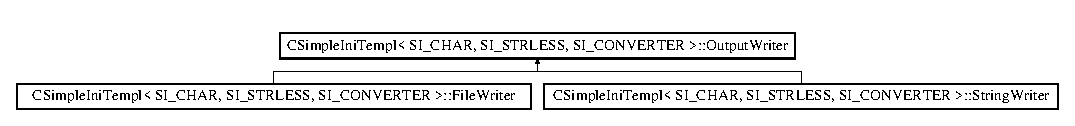
\includegraphics[height=1.244444cm]{a00020}
\end{center}
\end{figure}
\subsection*{Public Member Functions}
\begin{DoxyCompactItemize}
\item 
virtual void {\bfseries Write} (const char $\ast$a\+\_\+p\+Buf)=0\hypertarget{a00020_a48e5905a9defbe96d14f3068a383463d}{}\label{a00020_a48e5905a9defbe96d14f3068a383463d}

\end{DoxyCompactItemize}


\subsection{Detailed Description}
\subsubsection*{template$<$class S\+I\+\_\+\+C\+H\+AR, class S\+I\+\_\+\+S\+T\+R\+L\+E\+SS, class S\+I\+\_\+\+C\+O\+N\+V\+E\+R\+T\+ER$>$\\*
class C\+Simple\+Ini\+Templ$<$ S\+I\+\_\+\+C\+H\+A\+R, S\+I\+\_\+\+S\+T\+R\+L\+E\+S\+S, S\+I\+\_\+\+C\+O\+N\+V\+E\+R\+T\+E\+R $>$\+::\+Output\+Writer}

interface definition for the \hyperlink{a00020}{Output\+Writer} object to pass to \hyperlink{a00007_a5fea5d590edbb5eef694991c7c355915}{Save()} in order to output the I\+NI file data. 

The documentation for this class was generated from the following file\+:\begin{DoxyCompactItemize}
\item 
Simple\+Ini.\+h\end{DoxyCompactItemize}

\hypertarget{a00021}{}\section{fire\+:\+:Initializer$<$ Fire\+Tensor, Scalar, N $>$ Struct Template Reference}
\label{a00021}\index{fire\+::\+Initializer$<$ Fire\+Tensor, Scalar, N $>$@{fire\+::\+Initializer$<$ Fire\+Tensor, Scalar, N $>$}}


{\ttfamily \#include $<$Tensor\+Utils.\+hpp$>$}

\subsection*{Public Types}
\begin{DoxyCompactItemize}
\item 
\hypertarget{a00021_aeb5626b5276d5c021ba8971b2d524c45}{}typedef std\+::initializer\+\_\+list$<$ typename \hyperlink{a00021}{Initializer}$<$ Fire\+Tensor, Scalar, N-\/1 $>$\+::Init\+List $>$ {\bfseries Init\+List}\label{a00021_aeb5626b5276d5c021ba8971b2d524c45}

\end{DoxyCompactItemize}


\subsection{Detailed Description}
\subsubsection*{template$<$typename Fire\+Tensor, typename Scalar, int N$>$struct fire\+::\+Initializer$<$ Fire\+Tensor, Scalar, N $>$}

The following three templates set up the recursion necessary to express nexted std\+::initializer\+\_\+lists. We use this to accept tensor values and set them on the internal \hyperlink{a00047}{Tensor\+Provider} tensor instance. 

The documentation for this struct was generated from the following file\+:\begin{DoxyCompactItemize}
\item 
Tensor\+Utils.\+hpp\end{DoxyCompactItemize}

\hypertarget{a00022}{}\section{fire\+:\+:astrophysics\+:\+:Reaction Struct Reference}
\label{a00022}\index{fire\+::astrophysics\+::\+Reaction@{fire\+::astrophysics\+::\+Reaction}}


{\ttfamily \#include $<$Reaction.\+h$>$}

\subsection*{Public Member Functions}
\begin{DoxyCompactItemize}
\item 
void \hyperlink{a00022_a98b03c550c3926cb5c20f8a27a2ee1ed}{set\+Prefactor} (const double \&rho)
\item 
void \hyperlink{a00022_a671a0560e6843664cdae4d724b8645da}{set\+Rate} (array$<$ double, 6 $>$ temp\+Values)
\item 
void \hyperlink{a00022_a598fe411c64ab247e5d4f299b4a59b70}{set\+Rate} (const double \&temp)
\end{DoxyCompactItemize}
\subsection*{Public Attributes}
\begin{DoxyCompactItemize}
\item 
std\+::string \hyperlink{a00022_abb359091e992ad4cb4cde0faacf6021b}{name}
\item 
int \hyperlink{a00022_ab6d29b5c28ef33ea1d9219b70f02d98a}{reaction\+Group\+Class}
\item 
int \hyperlink{a00022_adb666fe2c511b5a5e86ebcd35ba7faa4}{reaction\+Group\+Member\+Index}
\item 
int \hyperlink{a00022_a581b5410f62a299f2262324d6c0199c7}{reaclib\+Class}
\item 
int \hyperlink{a00022_a86154569e16ef396c93cdf97c5eaf5b7}{num\+Reactants}
\item 
int \hyperlink{a00022_aa59b550e5dbdd34c9c563e7dfc2cbc1e}{num\+Products}
\item 
bool \hyperlink{a00022_a84165249a444a64bdfc41531fbe81cc0}{is\+Electron\+Capture}
\item 
bool \hyperlink{a00022_ae161628da753400b3d2256e2d10a02b9}{is\+Reverse}
\item 
double \hyperlink{a00022_a439daff55fecd97cafc96f204570376a}{statistical\+Factor}
\item 
double \hyperlink{a00022_a07f4db35c5d9bca2d5c5fc8529ec3801}{energy\+Release}
\item 
array$<$ double, 7 $>$ \hyperlink{a00022_aa6265e73f4d2c55441caf95e6eb6e656}{reaclib\+Rate\+Coeff}
\item 
array$<$ int, 4 $>$ \hyperlink{a00022_a74b96d4f5ff99d60adfb88b096a7e256}{reactantZ}
\item 
array$<$ int, 4 $>$ \hyperlink{a00022_a831dcae79d4ed842c9bbdf51ebdd137f}{reactantN}
\item 
array$<$ int, 4 $>$ \hyperlink{a00022_a0586d888e1f60d6371239af888f9158b}{productZ}
\item 
array$<$ int, 4 $>$ \hyperlink{a00022_a81251169f8dd972b6cdc285fbc42c331}{productN}
\item 
array$<$ int, 3 $>$ \hyperlink{a00022_ab13b0133b89c6531a1648b696324d804}{reactants}
\item 
array$<$ int, 3 $>$ \hyperlink{a00022_a5d0e77ebec059081aaafa5ba86df4c88}{products}
\item 
double \hyperlink{a00022_a5033228e6305beb4e8dd717d2f088d99}{prefactor}
\item 
double \hyperlink{a00022_a343553d449e3cca261f8ee166fa6b699}{rate}
\end{DoxyCompactItemize}


\subsection{Detailed Description}
This class represents a reaction, and specifically a nuclear reaction in the astrophysical case. This includes both forward reactions and backward (decay) reactions with one to four reacting bodies.

At the moment, this struct has an extremely bad design. However, it is worth noting that this is significantly better than what is currently used. There are several useful optimizations that will be added in time, such as using the \hyperlink{a00028}{Species} class and creating a new reaction group class. 

\subsection{Member Function Documentation}
\index{fire\+::astrophysics\+::\+Reaction@{fire\+::astrophysics\+::\+Reaction}!set\+Prefactor@{set\+Prefactor}}
\index{set\+Prefactor@{set\+Prefactor}!fire\+::astrophysics\+::\+Reaction@{fire\+::astrophysics\+::\+Reaction}}
\subsubsection[{\texorpdfstring{set\+Prefactor(const double \&rho)}{setPrefactor(const double \&rho)}}]{\setlength{\rightskip}{0pt plus 5cm}void fire\+::astrophysics\+::\+Reaction\+::set\+Prefactor (
\begin{DoxyParamCaption}
\item[{const double \&}]{rho}
\end{DoxyParamCaption}
)\hspace{0.3cm}{\ttfamily [inline]}}\hypertarget{a00022_a98b03c550c3926cb5c20f8a27a2ee1ed}{}\label{a00022_a98b03c550c3926cb5c20f8a27a2ee1ed}
The statistical prefactor that act as constant multipliers on this reaction. \[ p_s = s\rho^{(n_R -1)}. \] 
\begin{DoxyParams}{Parameters}
{\em the} & current density \\
\hline
\end{DoxyParams}
\index{fire\+::astrophysics\+::\+Reaction@{fire\+::astrophysics\+::\+Reaction}!set\+Rate@{set\+Rate}}
\index{set\+Rate@{set\+Rate}!fire\+::astrophysics\+::\+Reaction@{fire\+::astrophysics\+::\+Reaction}}
\subsubsection[{\texorpdfstring{set\+Rate(array$<$ double, 6 $>$ temp\+Values)}{setRate(array< double, 6 > tempValues)}}]{\setlength{\rightskip}{0pt plus 5cm}void fire\+::astrophysics\+::\+Reaction\+::set\+Rate (
\begin{DoxyParamCaption}
\item[{array$<$ double, 6 $>$}]{temp\+Values}
\end{DoxyParamCaption}
)\hspace{0.3cm}{\ttfamily [inline]}}\hypertarget{a00022_a671a0560e6843664cdae4d724b8645da}{}\label{a00022_a671a0560e6843664cdae4d724b8645da}
This operation computes and sets the reaction rate. This version is optimized to use pre-\/computed temperature values so that the costly exponentiation does not need to be repeated for each reaction if the temperature doesn\textquotesingle{}t change. 
\begin{DoxyParams}{Parameters}
{\em An} & array of all six temperature values used to compute the rate.\\
\hline
\end{DoxyParams}
The rate is computed by \[ R = p_s*\sum_k R_k \] where \[p_s\] is the prefactor (based on the statistical prefactor) and \[ R_k = \exp(p_1 + \frac{p_2}{T_9} + \frac{p_3}{T_9^{1/3}} + p_{4}T_9^{1/3} + p_{5}T_9 + p_{6}T_9^{5/3} + p_{7}\ln T_9). \]

$T_9$ is the the temperature in units of $10^9$ Kelvin. Note that p1 = reaclib\+Rate\+Coeff\mbox{[}0\mbox{]} since C++ is a zero-\/indexed language.

In general k may be greater than 1 in the summation for the rate, but in this work k = 1 and \[R = R_k\].

See\+: \char`\"{}\+Stars and Stellar Processes\char`\"{}, Mike Guidry, to be published Cambridge University Press. \index{fire\+::astrophysics\+::\+Reaction@{fire\+::astrophysics\+::\+Reaction}!set\+Rate@{set\+Rate}}
\index{set\+Rate@{set\+Rate}!fire\+::astrophysics\+::\+Reaction@{fire\+::astrophysics\+::\+Reaction}}
\subsubsection[{\texorpdfstring{set\+Rate(const double \&temp)}{setRate(const double \&temp)}}]{\setlength{\rightskip}{0pt plus 5cm}void fire\+::astrophysics\+::\+Reaction\+::set\+Rate (
\begin{DoxyParamCaption}
\item[{const double \&}]{temp}
\end{DoxyParamCaption}
)\hspace{0.3cm}{\ttfamily [inline]}}\hypertarget{a00022_a598fe411c64ab247e5d4f299b4a59b70}{}\label{a00022_a598fe411c64ab247e5d4f299b4a59b70}
This operation computes and sets the reaction rate. This version will use the provided temperature to compute all of the temperature coefficients. See the other version of this function for a more efficient version (which this function actually calls). 
\begin{DoxyParams}{Parameters}
{\em the} & temperature\\
\hline
\end{DoxyParams}
The rate is computed by \[ R = p_s*\sum_k R_k \] where \[p_s\] is the prefactor (based on the statistical prefactor) and \[ R_k = \exp(p_1 + \frac{p_2}{T_9} + \frac{p_3}{T_9^{1/3}} + p_{4}T_9^{1/3} + p_{5}T_9 + p_{6}T_9^{5/3} + p_{7}\ln T_9). \]

$T_9$ is the the temperature in units of $10^9$ Kelvin. Note that p1 = reaclib\+Rate\+Coeff\mbox{[}0\mbox{]} since C++ is a zero-\/indexed language.

In general k may be greater than 1 in the summation for the rate, but in this work k = 1 and \[R = R_k\].

See\+: \char`\"{}\+Stars and Stellar Processes\char`\"{}, Mike Guidry, to be published Cambridge University Press. 

\subsection{Member Data Documentation}
\index{fire\+::astrophysics\+::\+Reaction@{fire\+::astrophysics\+::\+Reaction}!energy\+Release@{energy\+Release}}
\index{energy\+Release@{energy\+Release}!fire\+::astrophysics\+::\+Reaction@{fire\+::astrophysics\+::\+Reaction}}
\subsubsection[{\texorpdfstring{energy\+Release}{energyRelease}}]{\setlength{\rightskip}{0pt plus 5cm}double fire\+::astrophysics\+::\+Reaction\+::energy\+Release}\hypertarget{a00022_a07f4db35c5d9bca2d5c5fc8529ec3801}{}\label{a00022_a07f4db35c5d9bca2d5c5fc8529ec3801}
The energy released by this reaction in electron volts. \index{fire\+::astrophysics\+::\+Reaction@{fire\+::astrophysics\+::\+Reaction}!is\+Electron\+Capture@{is\+Electron\+Capture}}
\index{is\+Electron\+Capture@{is\+Electron\+Capture}!fire\+::astrophysics\+::\+Reaction@{fire\+::astrophysics\+::\+Reaction}}
\subsubsection[{\texorpdfstring{is\+Electron\+Capture}{isElectronCapture}}]{\setlength{\rightskip}{0pt plus 5cm}bool fire\+::astrophysics\+::\+Reaction\+::is\+Electron\+Capture}\hypertarget{a00022_a84165249a444a64bdfc41531fbe81cc0}{}\label{a00022_a84165249a444a64bdfc41531fbe81cc0}
This is flag that designates whether or not the reaction captures an electron. \index{fire\+::astrophysics\+::\+Reaction@{fire\+::astrophysics\+::\+Reaction}!is\+Reverse@{is\+Reverse}}
\index{is\+Reverse@{is\+Reverse}!fire\+::astrophysics\+::\+Reaction@{fire\+::astrophysics\+::\+Reaction}}
\subsubsection[{\texorpdfstring{is\+Reverse}{isReverse}}]{\setlength{\rightskip}{0pt plus 5cm}bool fire\+::astrophysics\+::\+Reaction\+::is\+Reverse}\hypertarget{a00022_ae161628da753400b3d2256e2d10a02b9}{}\label{a00022_ae161628da753400b3d2256e2d10a02b9}
True if this reaction is a reverse reaction.

A\+SK M\+I\+K\+E! Why is this set to false by in F\+E\+RN\textquotesingle{}s load\+Reactions operation? \index{fire\+::astrophysics\+::\+Reaction@{fire\+::astrophysics\+::\+Reaction}!name@{name}}
\index{name@{name}!fire\+::astrophysics\+::\+Reaction@{fire\+::astrophysics\+::\+Reaction}}
\subsubsection[{\texorpdfstring{name}{name}}]{\setlength{\rightskip}{0pt plus 5cm}std\+::string fire\+::astrophysics\+::\+Reaction\+::name}\hypertarget{a00022_abb359091e992ad4cb4cde0faacf6021b}{}\label{a00022_abb359091e992ad4cb4cde0faacf6021b}
The name, or label, for the reaction. This should be of the form\+: \char`\"{}he4+he4+he4-\/-\/$>$c12\char`\"{} \index{fire\+::astrophysics\+::\+Reaction@{fire\+::astrophysics\+::\+Reaction}!num\+Products@{num\+Products}}
\index{num\+Products@{num\+Products}!fire\+::astrophysics\+::\+Reaction@{fire\+::astrophysics\+::\+Reaction}}
\subsubsection[{\texorpdfstring{num\+Products}{numProducts}}]{\setlength{\rightskip}{0pt plus 5cm}int fire\+::astrophysics\+::\+Reaction\+::num\+Products}\hypertarget{a00022_aa59b550e5dbdd34c9c563e7dfc2cbc1e}{}\label{a00022_aa59b550e5dbdd34c9c563e7dfc2cbc1e}
The number of products produced as a result of the reaction. \index{fire\+::astrophysics\+::\+Reaction@{fire\+::astrophysics\+::\+Reaction}!num\+Reactants@{num\+Reactants}}
\index{num\+Reactants@{num\+Reactants}!fire\+::astrophysics\+::\+Reaction@{fire\+::astrophysics\+::\+Reaction}}
\subsubsection[{\texorpdfstring{num\+Reactants}{numReactants}}]{\setlength{\rightskip}{0pt plus 5cm}int fire\+::astrophysics\+::\+Reaction\+::num\+Reactants}\hypertarget{a00022_a86154569e16ef396c93cdf97c5eaf5b7}{}\label{a00022_a86154569e16ef396c93cdf97c5eaf5b7}
The number of species in this reaction. \index{fire\+::astrophysics\+::\+Reaction@{fire\+::astrophysics\+::\+Reaction}!prefactor@{prefactor}}
\index{prefactor@{prefactor}!fire\+::astrophysics\+::\+Reaction@{fire\+::astrophysics\+::\+Reaction}}
\subsubsection[{\texorpdfstring{prefactor}{prefactor}}]{\setlength{\rightskip}{0pt plus 5cm}double fire\+::astrophysics\+::\+Reaction\+::prefactor}\hypertarget{a00022_a5033228e6305beb4e8dd717d2f088d99}{}\label{a00022_a5033228e6305beb4e8dd717d2f088d99}
The statistical prefactor that act as constant multipliers on this reaction. \[ p_s = s\rho^{(n_R -1)}. \] 
\begin{DoxyParams}{Parameters}
{\em the} & current density \\
\hline
\end{DoxyParams}
\index{fire\+::astrophysics\+::\+Reaction@{fire\+::astrophysics\+::\+Reaction}!productN@{productN}}
\index{productN@{productN}!fire\+::astrophysics\+::\+Reaction@{fire\+::astrophysics\+::\+Reaction}}
\subsubsection[{\texorpdfstring{productN}{productN}}]{\setlength{\rightskip}{0pt plus 5cm}array$<$int, 4$>$ fire\+::astrophysics\+::\+Reaction\+::productN}\hypertarget{a00022_a81251169f8dd972b6cdc285fbc42c331}{}\label{a00022_a81251169f8dd972b6cdc285fbc42c331}
The array of neutron numbers for the products in this reaction. \index{fire\+::astrophysics\+::\+Reaction@{fire\+::astrophysics\+::\+Reaction}!products@{products}}
\index{products@{products}!fire\+::astrophysics\+::\+Reaction@{fire\+::astrophysics\+::\+Reaction}}
\subsubsection[{\texorpdfstring{products}{products}}]{\setlength{\rightskip}{0pt plus 5cm}array$<$int, 3$>$ fire\+::astrophysics\+::\+Reaction\+::products}\hypertarget{a00022_a5d0e77ebec059081aaafa5ba86df4c88}{}\label{a00022_a5d0e77ebec059081aaafa5ba86df4c88}
The array of products to add to reac\+Vector.

No idea. A\+SK M\+I\+K\+E! This is used by the partial equilibrium code and may be useless for now. \index{fire\+::astrophysics\+::\+Reaction@{fire\+::astrophysics\+::\+Reaction}!productZ@{productZ}}
\index{productZ@{productZ}!fire\+::astrophysics\+::\+Reaction@{fire\+::astrophysics\+::\+Reaction}}
\subsubsection[{\texorpdfstring{productZ}{productZ}}]{\setlength{\rightskip}{0pt plus 5cm}array$<$int, 4$>$ fire\+::astrophysics\+::\+Reaction\+::productZ}\hypertarget{a00022_a0586d888e1f60d6371239af888f9158b}{}\label{a00022_a0586d888e1f60d6371239af888f9158b}
The array of atomic numbers for the products in this reaction. \index{fire\+::astrophysics\+::\+Reaction@{fire\+::astrophysics\+::\+Reaction}!rate@{rate}}
\index{rate@{rate}!fire\+::astrophysics\+::\+Reaction@{fire\+::astrophysics\+::\+Reaction}}
\subsubsection[{\texorpdfstring{rate}{rate}}]{\setlength{\rightskip}{0pt plus 5cm}double fire\+::astrophysics\+::\+Reaction\+::rate}\hypertarget{a00022_a343553d449e3cca261f8ee166fa6b699}{}\label{a00022_a343553d449e3cca261f8ee166fa6b699}
The reaction rate as described in \hyperlink{a00022_a671a0560e6843664cdae4d724b8645da}{set\+Rate()}. \index{fire\+::astrophysics\+::\+Reaction@{fire\+::astrophysics\+::\+Reaction}!reaclib\+Class@{reaclib\+Class}}
\index{reaclib\+Class@{reaclib\+Class}!fire\+::astrophysics\+::\+Reaction@{fire\+::astrophysics\+::\+Reaction}}
\subsubsection[{\texorpdfstring{reaclib\+Class}{reaclibClass}}]{\setlength{\rightskip}{0pt plus 5cm}int fire\+::astrophysics\+::\+Reaction\+::reaclib\+Class}\hypertarget{a00022_a581b5410f62a299f2262324d6c0199c7}{}\label{a00022_a581b5410f62a299f2262324d6c0199c7}
The class of this reaction in the R\+E\+A\+C\+L\+IB rate library. \index{fire\+::astrophysics\+::\+Reaction@{fire\+::astrophysics\+::\+Reaction}!reaclib\+Rate\+Coeff@{reaclib\+Rate\+Coeff}}
\index{reaclib\+Rate\+Coeff@{reaclib\+Rate\+Coeff}!fire\+::astrophysics\+::\+Reaction@{fire\+::astrophysics\+::\+Reaction}}
\subsubsection[{\texorpdfstring{reaclib\+Rate\+Coeff}{reaclibRateCoeff}}]{\setlength{\rightskip}{0pt plus 5cm}array$<$double,7$>$ fire\+::astrophysics\+::\+Reaction\+::reaclib\+Rate\+Coeff}\hypertarget{a00022_aa6265e73f4d2c55441caf95e6eb6e656}{}\label{a00022_aa6265e73f4d2c55441caf95e6eb6e656}
The array of R\+E\+A\+C\+L\+IB p-\/coefficients used in the parameterized computation of the rate. The rate is computed by \[ R = p_s*\sum_k R_k \] where \[p_s\] is the prefactor (based on the statistical prefactor) and \[ R_k = \exp(p_1 + \frac{p_2}{T_9} + \frac{p_3}{T_9^{1/3}} + p_{4}T_9^{1/3} + p_{5}T_9 + p_{6}T_9^{5/3} + p_{7}\ln T_9). \]

$T_9$ is the the temperature in units of $10^9$ Kelvin. Note that p1 = reaclib\+Rate\+Coeff\mbox{[}0\mbox{]} since C++ is a zero-\/indexed language.

In general k may be greater than 1 in the summation for the rate, but in this work k = 1 and \[R = R_k\].

See\+: \char`\"{}\+Stars and Stellar Processes\char`\"{}, Mike Guidry, to be published Cambridge University Press. \index{fire\+::astrophysics\+::\+Reaction@{fire\+::astrophysics\+::\+Reaction}!reactantN@{reactantN}}
\index{reactantN@{reactantN}!fire\+::astrophysics\+::\+Reaction@{fire\+::astrophysics\+::\+Reaction}}
\subsubsection[{\texorpdfstring{reactantN}{reactantN}}]{\setlength{\rightskip}{0pt plus 5cm}array$<$int, 4$>$ fire\+::astrophysics\+::\+Reaction\+::reactantN}\hypertarget{a00022_a831dcae79d4ed842c9bbdf51ebdd137f}{}\label{a00022_a831dcae79d4ed842c9bbdf51ebdd137f}
The array of neutron numbers for the reactants in this reaction. \index{fire\+::astrophysics\+::\+Reaction@{fire\+::astrophysics\+::\+Reaction}!reactants@{reactants}}
\index{reactants@{reactants}!fire\+::astrophysics\+::\+Reaction@{fire\+::astrophysics\+::\+Reaction}}
\subsubsection[{\texorpdfstring{reactants}{reactants}}]{\setlength{\rightskip}{0pt plus 5cm}array$<$int, 3$>$ fire\+::astrophysics\+::\+Reaction\+::reactants}\hypertarget{a00022_ab13b0133b89c6531a1648b696324d804}{}\label{a00022_ab13b0133b89c6531a1648b696324d804}
The array of reactants to subtract from reac\+Vector.

No idea. A\+SK M\+I\+K\+E! This is used by the partial equilibrium code and may be useless for now. \index{fire\+::astrophysics\+::\+Reaction@{fire\+::astrophysics\+::\+Reaction}!reactantZ@{reactantZ}}
\index{reactantZ@{reactantZ}!fire\+::astrophysics\+::\+Reaction@{fire\+::astrophysics\+::\+Reaction}}
\subsubsection[{\texorpdfstring{reactantZ}{reactantZ}}]{\setlength{\rightskip}{0pt plus 5cm}array$<$int, 4$>$ fire\+::astrophysics\+::\+Reaction\+::reactantZ}\hypertarget{a00022_a74b96d4f5ff99d60adfb88b096a7e256}{}\label{a00022_a74b96d4f5ff99d60adfb88b096a7e256}
The array of atomic numbers for the reactants in this reaction. \index{fire\+::astrophysics\+::\+Reaction@{fire\+::astrophysics\+::\+Reaction}!reaction\+Group\+Class@{reaction\+Group\+Class}}
\index{reaction\+Group\+Class@{reaction\+Group\+Class}!fire\+::astrophysics\+::\+Reaction@{fire\+::astrophysics\+::\+Reaction}}
\subsubsection[{\texorpdfstring{reaction\+Group\+Class}{reactionGroupClass}}]{\setlength{\rightskip}{0pt plus 5cm}int fire\+::astrophysics\+::\+Reaction\+::reaction\+Group\+Class}\hypertarget{a00022_ab6d29b5c28ef33ea1d9219b70f02d98a}{}\label{a00022_ab6d29b5c28ef33ea1d9219b70f02d98a}
The class of this reaction within its reaction group. \index{fire\+::astrophysics\+::\+Reaction@{fire\+::astrophysics\+::\+Reaction}!reaction\+Group\+Member\+Index@{reaction\+Group\+Member\+Index}}
\index{reaction\+Group\+Member\+Index@{reaction\+Group\+Member\+Index}!fire\+::astrophysics\+::\+Reaction@{fire\+::astrophysics\+::\+Reaction}}
\subsubsection[{\texorpdfstring{reaction\+Group\+Member\+Index}{reactionGroupMemberIndex}}]{\setlength{\rightskip}{0pt plus 5cm}int fire\+::astrophysics\+::\+Reaction\+::reaction\+Group\+Member\+Index}\hypertarget{a00022_adb666fe2c511b5a5e86ebcd35ba7faa4}{}\label{a00022_adb666fe2c511b5a5e86ebcd35ba7faa4}
The index of this reaction within the reaction group. \index{fire\+::astrophysics\+::\+Reaction@{fire\+::astrophysics\+::\+Reaction}!statistical\+Factor@{statistical\+Factor}}
\index{statistical\+Factor@{statistical\+Factor}!fire\+::astrophysics\+::\+Reaction@{fire\+::astrophysics\+::\+Reaction}}
\subsubsection[{\texorpdfstring{statistical\+Factor}{statisticalFactor}}]{\setlength{\rightskip}{0pt plus 5cm}double fire\+::astrophysics\+::\+Reaction\+::statistical\+Factor}\hypertarget{a00022_a439daff55fecd97cafc96f204570376a}{}\label{a00022_a439daff55fecd97cafc96f204570376a}
A statistical factor associated with this reaction that avoids double counting. It also accounts for the sign needed to designate whether or not the population is depleting or increasing. 

The documentation for this struct was generated from the following file\+:\begin{DoxyCompactItemize}
\item 
Reaction.\+h\end{DoxyCompactItemize}

\hypertarget{a00023}{}\section{fire\+:\+:Initializer$<$ Fire\+Tensor, Scalar, 1 $>$ Struct Template Reference}
\label{a00023}\index{fire\+::\+Initializer$<$ Fire\+Tensor, Scalar, 1 $>$@{fire\+::\+Initializer$<$ Fire\+Tensor, Scalar, 1 $>$}}
\subsection*{Public Types}
\begin{DoxyCompactItemize}
\item 
\hypertarget{a00023_ab08b58675de0070598ae477a509856c8}{}typedef std\+::initializer\+\_\+list$<$ Scalar $>$ {\bfseries Init\+List}\label{a00023_ab08b58675de0070598ae477a509856c8}

\end{DoxyCompactItemize}


The documentation for this struct was generated from the following file\+:\begin{DoxyCompactItemize}
\item 
Tensor\+Utils.\+hpp\end{DoxyCompactItemize}

\hypertarget{a00024}{}\section{S\+I\+\_\+\+ConvertA$<$ S\+I\+\_\+\+C\+H\+AR $>$ Class Template Reference}
\label{a00024}\index{S\+I\+\_\+\+Convert\+A$<$ S\+I\+\_\+\+C\+H\+A\+R $>$@{S\+I\+\_\+\+Convert\+A$<$ S\+I\+\_\+\+C\+H\+A\+R $>$}}


{\ttfamily \#include $<$Simple\+Ini.\+h$>$}

\subsection*{Public Member Functions}
\begin{DoxyCompactItemize}
\item 
{\bfseries S\+I\+\_\+\+ConvertA} (bool a\+\_\+b\+Store\+Is\+Utf8)\hypertarget{a00024_ab9c32530dc603974c3fdca06aad5b801}{}\label{a00024_ab9c32530dc603974c3fdca06aad5b801}

\item 
{\bfseries S\+I\+\_\+\+ConvertA} (const \hyperlink{a00024}{S\+I\+\_\+\+ConvertA} \&rhs)\hypertarget{a00024_a532fa9943ae417518e370a489bdea0f5}{}\label{a00024_a532fa9943ae417518e370a489bdea0f5}

\item 
\hyperlink{a00024}{S\+I\+\_\+\+ConvertA} \& {\bfseries operator=} (const \hyperlink{a00024}{S\+I\+\_\+\+ConvertA} \&rhs)\hypertarget{a00024_a4296011c45379c08309ce2b0709b387b}{}\label{a00024_a4296011c45379c08309ce2b0709b387b}

\item 
size\+\_\+t \hyperlink{a00024_a30ce0eee2556184d41130311d3c8cc84}{Size\+From\+Store} (const char $\ast$a\+\_\+p\+Input\+Data, size\+\_\+t a\+\_\+u\+Input\+Data\+Len)
\item 
bool \hyperlink{a00024_a5176a6dc2dc6482280e9a08dd3607f9e}{Convert\+From\+Store} (const char $\ast$a\+\_\+p\+Input\+Data, size\+\_\+t a\+\_\+u\+Input\+Data\+Len, S\+I\+\_\+\+C\+H\+AR $\ast$a\+\_\+p\+Output\+Data, size\+\_\+t a\+\_\+u\+Output\+Data\+Size)
\item 
size\+\_\+t \hyperlink{a00024_a39e7a8c49712c295b24ff2ae788c01c5}{Size\+To\+Store} (const S\+I\+\_\+\+C\+H\+AR $\ast$a\+\_\+p\+Input\+Data)
\item 
bool \hyperlink{a00024_a188fd6d6fcba6ba8d769e70e5fbea742}{Convert\+To\+Store} (const S\+I\+\_\+\+C\+H\+AR $\ast$a\+\_\+p\+Input\+Data, char $\ast$a\+\_\+p\+Output\+Data, size\+\_\+t a\+\_\+u\+Output\+Data\+Size)
\end{DoxyCompactItemize}


\subsection{Detailed Description}
\subsubsection*{template$<$class S\+I\+\_\+\+C\+H\+AR$>$\\*
class S\+I\+\_\+\+Convert\+A$<$ S\+I\+\_\+\+C\+H\+A\+R $>$}

Null conversion class for M\+B\+C\+S/\+U\+T\+F-\/8 to char (or equivalent). 

\subsection{Member Function Documentation}
\index{S\+I\+\_\+\+ConvertA@{S\+I\+\_\+\+ConvertA}!Convert\+From\+Store@{Convert\+From\+Store}}
\index{Convert\+From\+Store@{Convert\+From\+Store}!S\+I\+\_\+\+ConvertA@{S\+I\+\_\+\+ConvertA}}
\subsubsection[{\texorpdfstring{Convert\+From\+Store(const char $\ast$a\+\_\+p\+Input\+Data, size\+\_\+t a\+\_\+u\+Input\+Data\+Len, S\+I\+\_\+\+C\+H\+A\+R $\ast$a\+\_\+p\+Output\+Data, size\+\_\+t a\+\_\+u\+Output\+Data\+Size)}{ConvertFromStore(const char *a\_pInputData, size\_t a\_uInputDataLen, SI\_CHAR *a\_pOutputData, size\_t a\_uOutputDataSize)}}]{\setlength{\rightskip}{0pt plus 5cm}template$<$class S\+I\+\_\+\+C\+H\+AR $>$ bool {\bf S\+I\+\_\+\+ConvertA}$<$ S\+I\+\_\+\+C\+H\+AR $>$\+::Convert\+From\+Store (
\begin{DoxyParamCaption}
\item[{const char $\ast$}]{a\+\_\+p\+Input\+Data, }
\item[{size\+\_\+t}]{a\+\_\+u\+Input\+Data\+Len, }
\item[{S\+I\+\_\+\+C\+H\+AR $\ast$}]{a\+\_\+p\+Output\+Data, }
\item[{size\+\_\+t}]{a\+\_\+u\+Output\+Data\+Size}
\end{DoxyParamCaption}
)\hspace{0.3cm}{\ttfamily [inline]}}\hypertarget{a00024_a5176a6dc2dc6482280e9a08dd3607f9e}{}\label{a00024_a5176a6dc2dc6482280e9a08dd3607f9e}
Convert the input string from the storage format to S\+I\+\_\+\+C\+H\+AR. The storage format is always U\+T\+F-\/8 or M\+B\+CS.


\begin{DoxyParams}{Parameters}
{\em a\+\_\+p\+Input\+Data} & Data in storage format to be converted to S\+I\+\_\+\+C\+H\+AR. \\
\hline
{\em a\+\_\+u\+Input\+Data\+Len} & Length of storage format data in bytes. This must be the actual length of the data, including N\+U\+LL byte if N\+U\+LL terminated string is required. \\
\hline
{\em a\+\_\+p\+Output\+Data} & Pointer to the output buffer to received the converted data. \\
\hline
{\em a\+\_\+u\+Output\+Data\+Size} & Size of the output buffer in S\+I\+\_\+\+C\+H\+AR. \\
\hline
\end{DoxyParams}
\begin{DoxyReturn}{Returns}
true if all of the input data was successfully converted. 
\end{DoxyReturn}
\index{S\+I\+\_\+\+ConvertA@{S\+I\+\_\+\+ConvertA}!Convert\+To\+Store@{Convert\+To\+Store}}
\index{Convert\+To\+Store@{Convert\+To\+Store}!S\+I\+\_\+\+ConvertA@{S\+I\+\_\+\+ConvertA}}
\subsubsection[{\texorpdfstring{Convert\+To\+Store(const S\+I\+\_\+\+C\+H\+A\+R $\ast$a\+\_\+p\+Input\+Data, char $\ast$a\+\_\+p\+Output\+Data, size\+\_\+t a\+\_\+u\+Output\+Data\+Size)}{ConvertToStore(const SI\_CHAR *a\_pInputData, char *a\_pOutputData, size\_t a\_uOutputDataSize)}}]{\setlength{\rightskip}{0pt plus 5cm}template$<$class S\+I\+\_\+\+C\+H\+AR $>$ bool {\bf S\+I\+\_\+\+ConvertA}$<$ S\+I\+\_\+\+C\+H\+AR $>$\+::Convert\+To\+Store (
\begin{DoxyParamCaption}
\item[{const S\+I\+\_\+\+C\+H\+AR $\ast$}]{a\+\_\+p\+Input\+Data, }
\item[{char $\ast$}]{a\+\_\+p\+Output\+Data, }
\item[{size\+\_\+t}]{a\+\_\+u\+Output\+Data\+Size}
\end{DoxyParamCaption}
)\hspace{0.3cm}{\ttfamily [inline]}}\hypertarget{a00024_a188fd6d6fcba6ba8d769e70e5fbea742}{}\label{a00024_a188fd6d6fcba6ba8d769e70e5fbea742}
Convert the input string to the storage format of this data. The storage format is always U\+T\+F-\/8 or M\+B\+CS.


\begin{DoxyParams}{Parameters}
{\em a\+\_\+p\+Input\+Data} & N\+U\+LL terminated source string to convert. All of the data will be converted including the terminating N\+U\+LL character. \\
\hline
{\em a\+\_\+p\+Output\+Data} & Pointer to the buffer to receive the converted string. \\
\hline
{\em a\+\_\+u\+Output\+Data\+Size} & Size of the output buffer in char. \\
\hline
\end{DoxyParams}
\begin{DoxyReturn}{Returns}
true if all of the input data, including the terminating N\+U\+LL character was successfully converted. 
\end{DoxyReturn}
\index{S\+I\+\_\+\+ConvertA@{S\+I\+\_\+\+ConvertA}!Size\+From\+Store@{Size\+From\+Store}}
\index{Size\+From\+Store@{Size\+From\+Store}!S\+I\+\_\+\+ConvertA@{S\+I\+\_\+\+ConvertA}}
\subsubsection[{\texorpdfstring{Size\+From\+Store(const char $\ast$a\+\_\+p\+Input\+Data, size\+\_\+t a\+\_\+u\+Input\+Data\+Len)}{SizeFromStore(const char *a\_pInputData, size\_t a\_uInputDataLen)}}]{\setlength{\rightskip}{0pt plus 5cm}template$<$class S\+I\+\_\+\+C\+H\+AR $>$ size\+\_\+t {\bf S\+I\+\_\+\+ConvertA}$<$ S\+I\+\_\+\+C\+H\+AR $>$\+::Size\+From\+Store (
\begin{DoxyParamCaption}
\item[{const char $\ast$}]{a\+\_\+p\+Input\+Data, }
\item[{size\+\_\+t}]{a\+\_\+u\+Input\+Data\+Len}
\end{DoxyParamCaption}
)\hspace{0.3cm}{\ttfamily [inline]}}\hypertarget{a00024_a30ce0eee2556184d41130311d3c8cc84}{}\label{a00024_a30ce0eee2556184d41130311d3c8cc84}
Calculate the number of S\+I\+\_\+\+C\+H\+AR required for converting the input from the storage format. The storage format is always U\+T\+F-\/8 or M\+B\+CS.


\begin{DoxyParams}{Parameters}
{\em a\+\_\+p\+Input\+Data} & Data in storage format to be converted to S\+I\+\_\+\+C\+H\+AR. \\
\hline
{\em a\+\_\+u\+Input\+Data\+Len} & Length of storage format data in bytes. This must be the actual length of the data, including N\+U\+LL byte if N\+U\+LL terminated string is required. \\
\hline
\end{DoxyParams}
\begin{DoxyReturn}{Returns}
Number of S\+I\+\_\+\+C\+H\+AR required by the string when converted. If there are embedded N\+U\+LL bytes in the input data, only the string up and not including the N\+U\+LL byte will be converted. 

-\/1 cast to size\+\_\+t on a conversion error. 
\end{DoxyReturn}
\index{S\+I\+\_\+\+ConvertA@{S\+I\+\_\+\+ConvertA}!Size\+To\+Store@{Size\+To\+Store}}
\index{Size\+To\+Store@{Size\+To\+Store}!S\+I\+\_\+\+ConvertA@{S\+I\+\_\+\+ConvertA}}
\subsubsection[{\texorpdfstring{Size\+To\+Store(const S\+I\+\_\+\+C\+H\+A\+R $\ast$a\+\_\+p\+Input\+Data)}{SizeToStore(const SI\_CHAR *a\_pInputData)}}]{\setlength{\rightskip}{0pt plus 5cm}template$<$class S\+I\+\_\+\+C\+H\+AR $>$ size\+\_\+t {\bf S\+I\+\_\+\+ConvertA}$<$ S\+I\+\_\+\+C\+H\+AR $>$\+::Size\+To\+Store (
\begin{DoxyParamCaption}
\item[{const S\+I\+\_\+\+C\+H\+AR $\ast$}]{a\+\_\+p\+Input\+Data}
\end{DoxyParamCaption}
)\hspace{0.3cm}{\ttfamily [inline]}}\hypertarget{a00024_a39e7a8c49712c295b24ff2ae788c01c5}{}\label{a00024_a39e7a8c49712c295b24ff2ae788c01c5}
Calculate the number of char required by the storage format of this data. The storage format is always U\+T\+F-\/8 or M\+B\+CS.


\begin{DoxyParams}{Parameters}
{\em a\+\_\+p\+Input\+Data} & N\+U\+LL terminated string to calculate the number of bytes required to be converted to storage format. \\
\hline
\end{DoxyParams}
\begin{DoxyReturn}{Returns}
Number of bytes required by the string when converted to storage format. This size always includes space for the terminating N\+U\+LL character. 

-\/1 cast to size\+\_\+t on a conversion error. 
\end{DoxyReturn}


The documentation for this class was generated from the following file\+:\begin{DoxyCompactItemize}
\item 
Simple\+Ini.\+h\end{DoxyCompactItemize}

\hypertarget{a00025}{}\section{fire\+:\+:I\+Property\+Parser Class Reference}
\label{a00025}\index{fire\+::\+I\+Property\+Parser@{fire\+::\+I\+Property\+Parser}}


{\ttfamily \#include $<$I\+Property\+Parser.\+h$>$}

Inheritance diagram for fire\+:\+:I\+Property\+Parser\+:\begin{figure}[H]
\begin{center}
\leavevmode
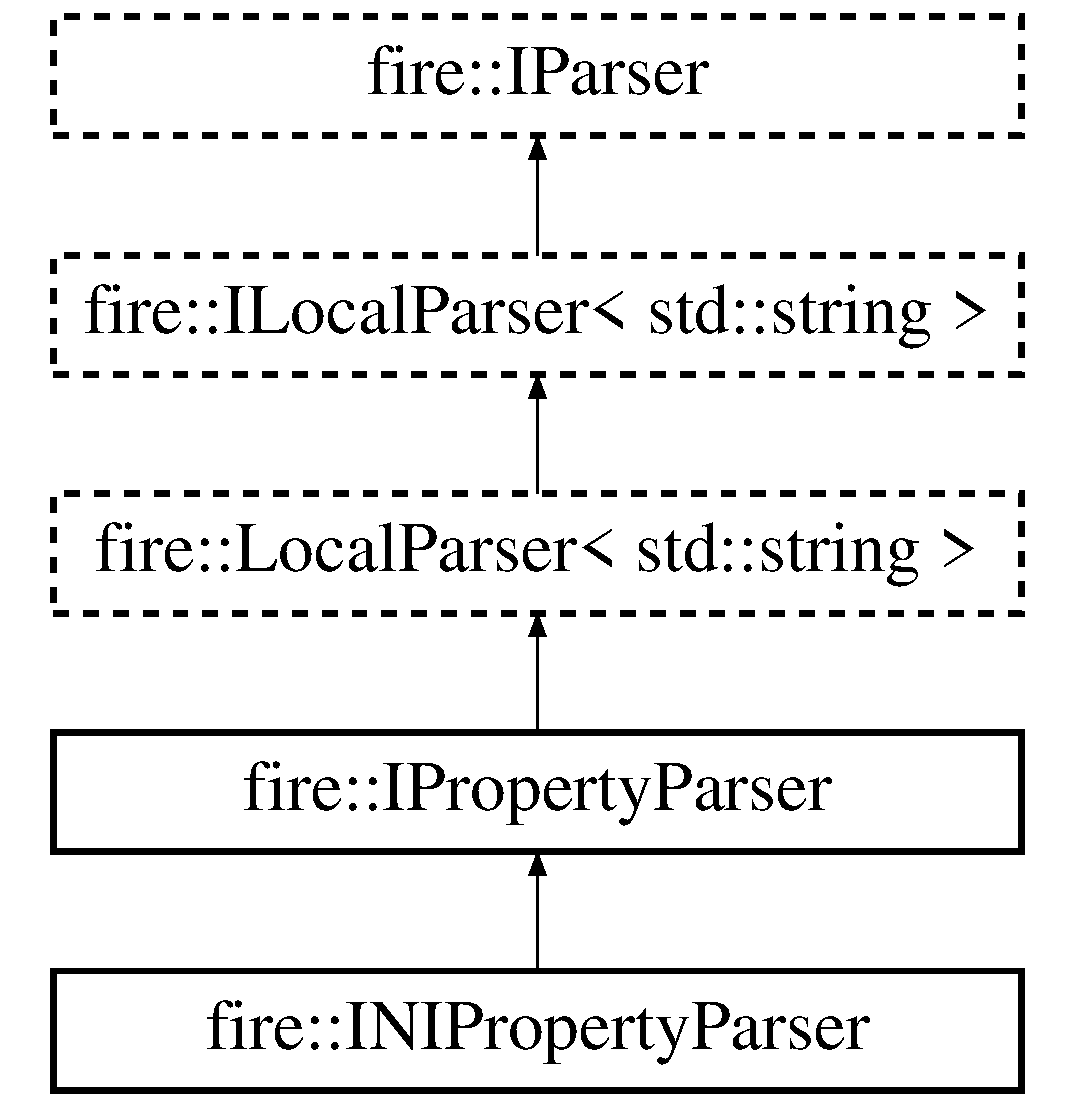
\includegraphics[height=5.000000cm]{a00025}
\end{center}
\end{figure}
\subsection*{Public Member Functions}
\begin{DoxyCompactItemize}
\item 
virtual const std\+::vector$<$ std\+::string $>$ \& \hyperlink{a00025_a34602687f9d1affac7bd842102d4a6aa}{get\+Property\+Block\+Names} ()=0
\item 
virtual const std\+::map$<$ std\+::string, std\+::string $>$ \& \hyperlink{a00025_a34201371cb36dd09e96a66242ececb86}{get\+Property\+Block} (const std\+::string \&name)=0
\end{DoxyCompactItemize}
\subsection*{Additional Inherited Members}


\subsection{Detailed Description}
This is an extension of the parser interface that focuses on parsing a set of properties. Properties are returned in blocks represented by maps.. 

\subsection{Member Function Documentation}
\hypertarget{a00025_a34201371cb36dd09e96a66242ececb86}{}\index{fire\+::\+I\+Property\+Parser@{fire\+::\+I\+Property\+Parser}!get\+Property\+Block@{get\+Property\+Block}}
\index{get\+Property\+Block@{get\+Property\+Block}!fire\+::\+I\+Property\+Parser@{fire\+::\+I\+Property\+Parser}}
\subsubsection[{get\+Property\+Block(const std\+::string \&name)=0}]{\setlength{\rightskip}{0pt plus 5cm}virtual const std\+::map$<$std\+::string, std\+::string$>$\& fire\+::\+I\+Property\+Parser\+::get\+Property\+Block (
\begin{DoxyParamCaption}
\item[{const std\+::string \&}]{name}
\end{DoxyParamCaption}
)\hspace{0.3cm}{\ttfamily [pure virtual]}}\label{a00025_a34201371cb36dd09e96a66242ececb86}
This operation returns the property block with the given name. 
\begin{DoxyParams}{Parameters}
{\em name} & the block name \\
\hline
\end{DoxyParams}
\begin{DoxyReturn}{Returns}
the property block with the given name 
\end{DoxyReturn}


Implemented in \hyperlink{a00020_a3591312590a66659ebd377cdde9ab9ad}{fire\+::\+I\+N\+I\+Property\+Parser}.

\hypertarget{a00025_a34602687f9d1affac7bd842102d4a6aa}{}\index{fire\+::\+I\+Property\+Parser@{fire\+::\+I\+Property\+Parser}!get\+Property\+Block\+Names@{get\+Property\+Block\+Names}}
\index{get\+Property\+Block\+Names@{get\+Property\+Block\+Names}!fire\+::\+I\+Property\+Parser@{fire\+::\+I\+Property\+Parser}}
\subsubsection[{get\+Property\+Block\+Names()=0}]{\setlength{\rightskip}{0pt plus 5cm}virtual const std\+::vector$<$std\+::string$>$\& fire\+::\+I\+Property\+Parser\+::get\+Property\+Block\+Names (
\begin{DoxyParamCaption}
{}
\end{DoxyParamCaption}
)\hspace{0.3cm}{\ttfamily [pure virtual]}}\label{a00025_a34602687f9d1affac7bd842102d4a6aa}
This operation returns the names of the property blocks parsed from the source. \begin{DoxyReturn}{Returns}
the block names 
\end{DoxyReturn}


Implemented in \hyperlink{a00020_aed0f1f47111794659564dcddb4d25bc6}{fire\+::\+I\+N\+I\+Property\+Parser}.



The documentation for this class was generated from the following file\+:\begin{DoxyCompactItemize}
\item 
I\+Property\+Parser.\+h\end{DoxyCompactItemize}

\hypertarget{a00026}{}\section{fire\+:\+:I\+Stepper Class Reference}
\label{a00026}\index{fire\+::\+I\+Stepper@{fire\+::\+I\+Stepper}}


{\ttfamily \#include $<$I\+Stepper.\+h$>$}

Inheritance diagram for fire\+:\+:I\+Stepper\+:\begin{figure}[H]
\begin{center}
\leavevmode
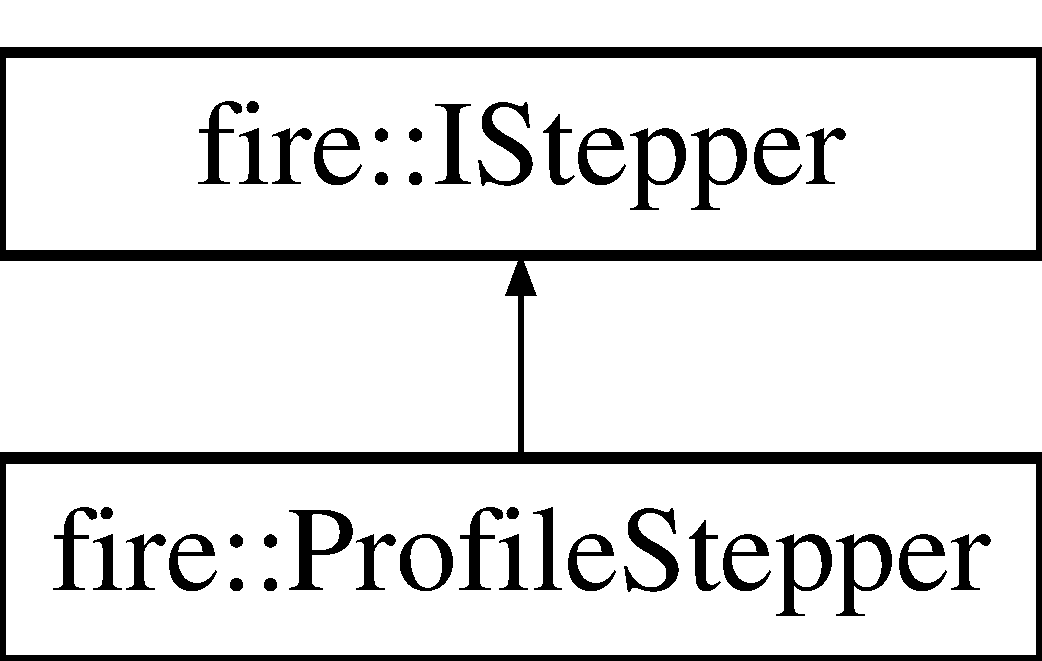
\includegraphics[height=2.000000cm]{a00026}
\end{center}
\end{figure}
\subsection*{Public Member Functions}
\begin{DoxyCompactItemize}
\item 
virtual double \hyperlink{a00026_a7f709d1462a2a3b8bd8214cc681ca26e}{get\+Step} ()=0
\item 
virtual double \hyperlink{a00026_a43027c0c268afcd59db8815c2e2c41ea}{get\+Step\+Size\+At\+Stage} (int i)=0
\item 
virtual void \hyperlink{a00026_a44dfccb90ee5ef6e080b54113c215458}{update\+Step} ()=0
\item 
virtual void \hyperlink{a00026_a3a5099cd0f3c874e56c33cb8f13b8f3b}{set\+Initial\+Step} (double initial\+Step)=0
\item 
virtual double \hyperlink{a00026_a49df3a2ac05cebaf2baf387b66d19272}{get\+Initial\+Step} ()=0
\item 
virtual void \hyperlink{a00026_add76974a7b6fbbc93916270a376c461e}{set\+Final\+Step} (double final\+Step)=0
\item 
virtual double \hyperlink{a00026_ab234d9f032e02668aededf1c22e8c0a9}{get\+Final\+Step} ()=0
\item 
virtual void \hyperlink{a00026_a69c262f248511efcd271be1724a41ad9}{set\+Initial\+Stepsize} (double step\+Size)=0
\item 
virtual double \hyperlink{a00026_afb777e62386b25e5a38d59af54972690}{get\+Initial\+Stepsize} ()=0
\item 
virtual \hyperlink{a00026_ac8ec460d35512e2e039396d5192eb57e}{$\sim$\+I\+Stepper} ()
\end{DoxyCompactItemize}


\subsection{Detailed Description}
This is an interface for managing discrete steps as required by Initial Value Problem Integrators. \hyperlink{a00026}{I\+Stepper} implementations track both the step and the stepsize. In the case of time-\/dependent initial value problems, implementations would be called \char`\"{}time steppers\char`\"{} and would be responsible for computing both the present time (the step) and the step between the present size and the next (the step size). In purely spatial or otherwise on-\/temporal problems, the step represents the current value of the independent variable and the step size represents the distance between the present and next steps.

This interface is designed for single-\/ and multi-\/stage solvers, such as Runge-\/\+Kutta solvers. 

\subsection{Constructor \& Destructor Documentation}
\hypertarget{a00026_ac8ec460d35512e2e039396d5192eb57e}{}\index{fire\+::\+I\+Stepper@{fire\+::\+I\+Stepper}!````~I\+Stepper@{$\sim$\+I\+Stepper}}
\index{````~I\+Stepper@{$\sim$\+I\+Stepper}!fire\+::\+I\+Stepper@{fire\+::\+I\+Stepper}}
\subsubsection[{$\sim$\+I\+Stepper()}]{\setlength{\rightskip}{0pt plus 5cm}virtual fire\+::\+I\+Stepper\+::$\sim$\+I\+Stepper (
\begin{DoxyParamCaption}
{}
\end{DoxyParamCaption}
)\hspace{0.3cm}{\ttfamily [inline]}, {\ttfamily [virtual]}}\label{a00026_ac8ec460d35512e2e039396d5192eb57e}
Virtual Destructor 

\subsection{Member Function Documentation}
\hypertarget{a00026_ab234d9f032e02668aededf1c22e8c0a9}{}\index{fire\+::\+I\+Stepper@{fire\+::\+I\+Stepper}!get\+Final\+Step@{get\+Final\+Step}}
\index{get\+Final\+Step@{get\+Final\+Step}!fire\+::\+I\+Stepper@{fire\+::\+I\+Stepper}}
\subsubsection[{get\+Final\+Step()=0}]{\setlength{\rightskip}{0pt plus 5cm}virtual double fire\+::\+I\+Stepper\+::get\+Final\+Step (
\begin{DoxyParamCaption}
{}
\end{DoxyParamCaption}
)\hspace{0.3cm}{\ttfamily [pure virtual]}}\label{a00026_ab234d9f032e02668aededf1c22e8c0a9}
This operation returns the final step for the stepper. \begin{DoxyReturn}{Returns}
the final step 
\end{DoxyReturn}


Implemented in \hyperlink{a00031_ae6f257aca7b3bb62a851169a01bcaacf}{fire\+::\+Profile\+Stepper}.

\hypertarget{a00026_a49df3a2ac05cebaf2baf387b66d19272}{}\index{fire\+::\+I\+Stepper@{fire\+::\+I\+Stepper}!get\+Initial\+Step@{get\+Initial\+Step}}
\index{get\+Initial\+Step@{get\+Initial\+Step}!fire\+::\+I\+Stepper@{fire\+::\+I\+Stepper}}
\subsubsection[{get\+Initial\+Step()=0}]{\setlength{\rightskip}{0pt plus 5cm}virtual double fire\+::\+I\+Stepper\+::get\+Initial\+Step (
\begin{DoxyParamCaption}
{}
\end{DoxyParamCaption}
)\hspace{0.3cm}{\ttfamily [pure virtual]}}\label{a00026_a49df3a2ac05cebaf2baf387b66d19272}
This operation returns the initial step for the stepper. \begin{DoxyReturn}{Returns}
the initial step 
\end{DoxyReturn}


Implemented in \hyperlink{a00031_af24660fa4bd027f877d5c1bdeb286cf5}{fire\+::\+Profile\+Stepper}.

\hypertarget{a00026_afb777e62386b25e5a38d59af54972690}{}\index{fire\+::\+I\+Stepper@{fire\+::\+I\+Stepper}!get\+Initial\+Stepsize@{get\+Initial\+Stepsize}}
\index{get\+Initial\+Stepsize@{get\+Initial\+Stepsize}!fire\+::\+I\+Stepper@{fire\+::\+I\+Stepper}}
\subsubsection[{get\+Initial\+Stepsize()=0}]{\setlength{\rightskip}{0pt plus 5cm}virtual double fire\+::\+I\+Stepper\+::get\+Initial\+Stepsize (
\begin{DoxyParamCaption}
{}
\end{DoxyParamCaption}
)\hspace{0.3cm}{\ttfamily [pure virtual]}}\label{a00026_afb777e62386b25e5a38d59af54972690}
This operation gets the initial step size for the stepper \begin{DoxyReturn}{Returns}
the initial step size 
\end{DoxyReturn}


Implemented in \hyperlink{a00031_a86e7035366907a08a36722655746271e}{fire\+::\+Profile\+Stepper}.

\hypertarget{a00026_a7f709d1462a2a3b8bd8214cc681ca26e}{}\index{fire\+::\+I\+Stepper@{fire\+::\+I\+Stepper}!get\+Step@{get\+Step}}
\index{get\+Step@{get\+Step}!fire\+::\+I\+Stepper@{fire\+::\+I\+Stepper}}
\subsubsection[{get\+Step()=0}]{\setlength{\rightskip}{0pt plus 5cm}virtual double fire\+::\+I\+Stepper\+::get\+Step (
\begin{DoxyParamCaption}
{}
\end{DoxyParamCaption}
)\hspace{0.3cm}{\ttfamily [pure virtual]}}\label{a00026_a7f709d1462a2a3b8bd8214cc681ca26e}
This operation returns the step value for the current step. \begin{DoxyReturn}{Returns}
the step value 
\end{DoxyReturn}


Implemented in \hyperlink{a00031_a9096ad65a3fcf63678b600cbe0c33961}{fire\+::\+Profile\+Stepper}.

\hypertarget{a00026_a43027c0c268afcd59db8815c2e2c41ea}{}\index{fire\+::\+I\+Stepper@{fire\+::\+I\+Stepper}!get\+Step\+Size\+At\+Stage@{get\+Step\+Size\+At\+Stage}}
\index{get\+Step\+Size\+At\+Stage@{get\+Step\+Size\+At\+Stage}!fire\+::\+I\+Stepper@{fire\+::\+I\+Stepper}}
\subsubsection[{get\+Step\+Size\+At\+Stage(int i)=0}]{\setlength{\rightskip}{0pt plus 5cm}virtual double fire\+::\+I\+Stepper\+::get\+Step\+Size\+At\+Stage (
\begin{DoxyParamCaption}
\item[{int}]{i}
\end{DoxyParamCaption}
)\hspace{0.3cm}{\ttfamily [pure virtual]}}\label{a00026_a43027c0c268afcd59db8815c2e2c41ea}
This operation returns the step size for the given stage. 
\begin{DoxyParams}{Parameters}
{\em the} & stage of the solver for which the stepsize should be computed \\
\hline
\end{DoxyParams}
\begin{DoxyReturn}{Returns}
the step size 
\end{DoxyReturn}


Implemented in \hyperlink{a00031_adaa1a23c068977ecc6809dd8eecab49d}{fire\+::\+Profile\+Stepper}.

\hypertarget{a00026_add76974a7b6fbbc93916270a376c461e}{}\index{fire\+::\+I\+Stepper@{fire\+::\+I\+Stepper}!set\+Final\+Step@{set\+Final\+Step}}
\index{set\+Final\+Step@{set\+Final\+Step}!fire\+::\+I\+Stepper@{fire\+::\+I\+Stepper}}
\subsubsection[{set\+Final\+Step(double final\+Step)=0}]{\setlength{\rightskip}{0pt plus 5cm}virtual void fire\+::\+I\+Stepper\+::set\+Final\+Step (
\begin{DoxyParamCaption}
\item[{double}]{final\+Step}
\end{DoxyParamCaption}
)\hspace{0.3cm}{\ttfamily [pure virtual]}}\label{a00026_add76974a7b6fbbc93916270a376c461e}
This operation sets the final step for the stepper. 
\begin{DoxyParams}{Parameters}
{\em final\+Step} & the final step \\
\hline
\end{DoxyParams}


Implemented in \hyperlink{a00031_af8203296b4f3bef53bafab7cb654cc97}{fire\+::\+Profile\+Stepper}.

\hypertarget{a00026_a3a5099cd0f3c874e56c33cb8f13b8f3b}{}\index{fire\+::\+I\+Stepper@{fire\+::\+I\+Stepper}!set\+Initial\+Step@{set\+Initial\+Step}}
\index{set\+Initial\+Step@{set\+Initial\+Step}!fire\+::\+I\+Stepper@{fire\+::\+I\+Stepper}}
\subsubsection[{set\+Initial\+Step(double initial\+Step)=0}]{\setlength{\rightskip}{0pt plus 5cm}virtual void fire\+::\+I\+Stepper\+::set\+Initial\+Step (
\begin{DoxyParamCaption}
\item[{double}]{initial\+Step}
\end{DoxyParamCaption}
)\hspace{0.3cm}{\ttfamily [pure virtual]}}\label{a00026_a3a5099cd0f3c874e56c33cb8f13b8f3b}
This operation sets the initial step for the stepper. 
\begin{DoxyParams}{Parameters}
{\em initial\+Step} & the initial step \\
\hline
\end{DoxyParams}


Implemented in \hyperlink{a00031_adf2f78648d9539282225117c0fd243af}{fire\+::\+Profile\+Stepper}.

\hypertarget{a00026_a69c262f248511efcd271be1724a41ad9}{}\index{fire\+::\+I\+Stepper@{fire\+::\+I\+Stepper}!set\+Initial\+Stepsize@{set\+Initial\+Stepsize}}
\index{set\+Initial\+Stepsize@{set\+Initial\+Stepsize}!fire\+::\+I\+Stepper@{fire\+::\+I\+Stepper}}
\subsubsection[{set\+Initial\+Stepsize(double step\+Size)=0}]{\setlength{\rightskip}{0pt plus 5cm}virtual void fire\+::\+I\+Stepper\+::set\+Initial\+Stepsize (
\begin{DoxyParamCaption}
\item[{double}]{step\+Size}
\end{DoxyParamCaption}
)\hspace{0.3cm}{\ttfamily [pure virtual]}}\label{a00026_a69c262f248511efcd271be1724a41ad9}
This operation sets the initial step size for the stepper 
\begin{DoxyParams}{Parameters}
{\em the} & initial step size \\
\hline
\end{DoxyParams}


Implemented in \hyperlink{a00031_a55c44fd97d8b6a474243ad0da48b039d}{fire\+::\+Profile\+Stepper}.

\hypertarget{a00026_a44dfccb90ee5ef6e080b54113c215458}{}\index{fire\+::\+I\+Stepper@{fire\+::\+I\+Stepper}!update\+Step@{update\+Step}}
\index{update\+Step@{update\+Step}!fire\+::\+I\+Stepper@{fire\+::\+I\+Stepper}}
\subsubsection[{update\+Step()=0}]{\setlength{\rightskip}{0pt plus 5cm}virtual void fire\+::\+I\+Stepper\+::update\+Step (
\begin{DoxyParamCaption}
{}
\end{DoxyParamCaption}
)\hspace{0.3cm}{\ttfamily [pure virtual]}}\label{a00026_a44dfccb90ee5ef6e080b54113c215458}
This operation replaces the current step and stepsize with the next step and stepsize values. 

Implemented in \hyperlink{a00031_a2c13fd4da5550f1e58df2b54bbfe4c2c}{fire\+::\+Profile\+Stepper}.



The documentation for this class was generated from the following file\+:\begin{DoxyCompactItemize}
\item 
I\+Stepper.\+h\end{DoxyCompactItemize}

\hypertarget{a00027}{}\section{S\+I\+\_\+\+Generic\+No\+Case$<$ S\+I\+\_\+\+C\+H\+AR $>$ Struct Template Reference}
\label{a00027}\index{S\+I\+\_\+\+Generic\+No\+Case$<$ S\+I\+\_\+\+C\+H\+A\+R $>$@{S\+I\+\_\+\+Generic\+No\+Case$<$ S\+I\+\_\+\+C\+H\+A\+R $>$}}


{\ttfamily \#include $<$Simple\+Ini.\+h$>$}

\subsection*{Public Member Functions}
\begin{DoxyCompactItemize}
\item 
S\+I\+\_\+\+C\+H\+AR {\bfseries locase} (S\+I\+\_\+\+C\+H\+AR ch) const \hypertarget{a00027_adc6bb2ca8960d24913b598a2f3085e7c}{}\label{a00027_adc6bb2ca8960d24913b598a2f3085e7c}

\item 
bool {\bfseries operator()} (const S\+I\+\_\+\+C\+H\+AR $\ast$p\+Left, const S\+I\+\_\+\+C\+H\+AR $\ast$p\+Right) const \hypertarget{a00027_aa8014f86b3d74b2cd0f6e9b6ccc43426}{}\label{a00027_aa8014f86b3d74b2cd0f6e9b6ccc43426}

\end{DoxyCompactItemize}


\subsection{Detailed Description}
\subsubsection*{template$<$class S\+I\+\_\+\+C\+H\+AR$>$\\*
struct S\+I\+\_\+\+Generic\+No\+Case$<$ S\+I\+\_\+\+C\+H\+A\+R $>$}

Generic A\+S\+C\+II case-\/insensitive less than comparison. This class returns numerically ordered A\+S\+C\+II case-\/insensitive text for all possible sizes and types of S\+I\+\_\+\+C\+H\+AR. It is not safe for M\+B\+CS text comparison where A\+S\+C\+II A-\/Z characters are used in the encoding of multi-\/byte characters. 

The documentation for this struct was generated from the following file\+:\begin{DoxyCompactItemize}
\item 
Simple\+Ini.\+h\end{DoxyCompactItemize}

\hypertarget{a00028}{}\section{fire\+:\+:astrophysics\+:\+:Species Struct Reference}
\label{a00028}\index{fire\+::astrophysics\+::\+Species@{fire\+::astrophysics\+::\+Species}}


{\ttfamily \#include $<$Species.\+h$>$}

\subsection*{Public Member Functions}
\begin{DoxyCompactItemize}
\item 
\hyperlink{a00028_ac3c237025b5bcd786519dfbf398f86d3}{Species} (const std\+::vector$<$ std\+::string $>$ \&values)
\end{DoxyCompactItemize}
\subsection*{Public Attributes}
\begin{DoxyCompactItemize}
\item 
const std\+::string \hyperlink{a00028_a4aea10c6b155eaeeb52dedcef2dcf849}{name}
\item 
const int \hyperlink{a00028_a403a85b9ffb625643b0bd5cf2e944376}{mass\+Number}
\item 
const int \hyperlink{a00028_a01796faa4262d2225c4cf3b714afde81}{atomic\+Number}
\item 
const int \hyperlink{a00028_acd295953eb640a1354df0be96e63f1cd}{neutron\+Number}
\item 
double \hyperlink{a00028_aa23c930af303e0c2b09491b18888855b}{mass\+Fraction}
\item 
const double \hyperlink{a00028_a3fd8c01bcbb27c20fb80cf9a9e6e1f66}{mass\+Excess}
\end{DoxyCompactItemize}


\subsection{Detailed Description}
This class represents a standard nuclear species within astrophysics such as Helium or Carbon. The mass fraction is the only value on this struct which can be changed.

This class is composed of const-\/qualified members because atomic parameters are immutable. The amount of a species present in a given context varies though. 

\subsection{Constructor \& Destructor Documentation}
\index{fire\+::astrophysics\+::\+Species@{fire\+::astrophysics\+::\+Species}!Species@{Species}}
\index{Species@{Species}!fire\+::astrophysics\+::\+Species@{fire\+::astrophysics\+::\+Species}}
\subsubsection[{\texorpdfstring{Species(const std\+::vector$<$ std\+::string $>$ \&values)}{Species(const std::vector< std::string > \&values)}}]{\setlength{\rightskip}{0pt plus 5cm}fire\+::astrophysics\+::\+Species\+::\+Species (
\begin{DoxyParamCaption}
\item[{const std\+::vector$<$ std\+::string $>$ \&}]{values}
\end{DoxyParamCaption}
)\hspace{0.3cm}{\ttfamily [inline]}}\hypertarget{a00028_ac3c237025b5bcd786519dfbf398f86d3}{}\label{a00028_ac3c237025b5bcd786519dfbf398f86d3}
The constructor. This class is meant to be initialized from a vector of data created by reading a line from a network file. The vector should have the following entries\+: v\mbox{[}0\mbox{]} -\/ The name v\mbox{[}1\mbox{]} -\/ The mass number v\mbox{[}2\mbox{]} -\/ The atomic number v\mbox{[}3\mbox{]} -\/ The neutron number v\mbox{[}4\mbox{]} -\/ The mass fraction v\mbox{[}5\mbox{]} -\/ The mass excess 
\begin{DoxyParams}{Parameters}
{\em a} & vector with entries for each of the data members in this class as described above. \\
\hline
\end{DoxyParams}


\subsection{Member Data Documentation}
\index{fire\+::astrophysics\+::\+Species@{fire\+::astrophysics\+::\+Species}!atomic\+Number@{atomic\+Number}}
\index{atomic\+Number@{atomic\+Number}!fire\+::astrophysics\+::\+Species@{fire\+::astrophysics\+::\+Species}}
\subsubsection[{\texorpdfstring{atomic\+Number}{atomicNumber}}]{\setlength{\rightskip}{0pt plus 5cm}const int fire\+::astrophysics\+::\+Species\+::atomic\+Number}\hypertarget{a00028_a01796faa4262d2225c4cf3b714afde81}{}\label{a00028_a01796faa4262d2225c4cf3b714afde81}
The total number of protons in the nucleus of this species. Also known as the proton number. \index{fire\+::astrophysics\+::\+Species@{fire\+::astrophysics\+::\+Species}!mass\+Excess@{mass\+Excess}}
\index{mass\+Excess@{mass\+Excess}!fire\+::astrophysics\+::\+Species@{fire\+::astrophysics\+::\+Species}}
\subsubsection[{\texorpdfstring{mass\+Excess}{massExcess}}]{\setlength{\rightskip}{0pt plus 5cm}const double fire\+::astrophysics\+::\+Species\+::mass\+Excess}\hypertarget{a00028_a3fd8c01bcbb27c20fb80cf9a9e6e1f66}{}\label{a00028_a3fd8c01bcbb27c20fb80cf9a9e6e1f66}
The difference between the actual mass of this species and the mass number. \index{fire\+::astrophysics\+::\+Species@{fire\+::astrophysics\+::\+Species}!mass\+Fraction@{mass\+Fraction}}
\index{mass\+Fraction@{mass\+Fraction}!fire\+::astrophysics\+::\+Species@{fire\+::astrophysics\+::\+Species}}
\subsubsection[{\texorpdfstring{mass\+Fraction}{massFraction}}]{\setlength{\rightskip}{0pt plus 5cm}double fire\+::astrophysics\+::\+Species\+::mass\+Fraction}\hypertarget{a00028_aa23c930af303e0c2b09491b18888855b}{}\label{a00028_aa23c930af303e0c2b09491b18888855b}
The fraction of the total mass of the system that is composed of this species. The quantity is normalized to 1.\+0. It is sometimes called the \char`\"{}abundance\char`\"{} as well. \index{fire\+::astrophysics\+::\+Species@{fire\+::astrophysics\+::\+Species}!mass\+Number@{mass\+Number}}
\index{mass\+Number@{mass\+Number}!fire\+::astrophysics\+::\+Species@{fire\+::astrophysics\+::\+Species}}
\subsubsection[{\texorpdfstring{mass\+Number}{massNumber}}]{\setlength{\rightskip}{0pt plus 5cm}const int fire\+::astrophysics\+::\+Species\+::mass\+Number}\hypertarget{a00028_a403a85b9ffb625643b0bd5cf2e944376}{}\label{a00028_a403a85b9ffb625643b0bd5cf2e944376}
The total number of nucleons, equal to the sum of the atomic and neutron numbers, in the nucleus of this species. \index{fire\+::astrophysics\+::\+Species@{fire\+::astrophysics\+::\+Species}!name@{name}}
\index{name@{name}!fire\+::astrophysics\+::\+Species@{fire\+::astrophysics\+::\+Species}}
\subsubsection[{\texorpdfstring{name}{name}}]{\setlength{\rightskip}{0pt plus 5cm}const std\+::string fire\+::astrophysics\+::\+Species\+::name}\hypertarget{a00028_a4aea10c6b155eaeeb52dedcef2dcf849}{}\label{a00028_a4aea10c6b155eaeeb52dedcef2dcf849}
The name of this species. \index{fire\+::astrophysics\+::\+Species@{fire\+::astrophysics\+::\+Species}!neutron\+Number@{neutron\+Number}}
\index{neutron\+Number@{neutron\+Number}!fire\+::astrophysics\+::\+Species@{fire\+::astrophysics\+::\+Species}}
\subsubsection[{\texorpdfstring{neutron\+Number}{neutronNumber}}]{\setlength{\rightskip}{0pt plus 5cm}const int fire\+::astrophysics\+::\+Species\+::neutron\+Number}\hypertarget{a00028_acd295953eb640a1354df0be96e63f1cd}{}\label{a00028_acd295953eb640a1354df0be96e63f1cd}
The total number of neutrons in the nucleus of this species. 

The documentation for this struct was generated from the following file\+:\begin{DoxyCompactItemize}
\item 
Species.\+h\end{DoxyCompactItemize}

\hypertarget{a00029}{}\section{fire\+:\+:String\+Caster$<$ T $>$ Struct Template Reference}
\label{a00029}\index{fire\+::\+String\+Caster$<$ T $>$@{fire\+::\+String\+Caster$<$ T $>$}}


{\ttfamily \#include $<$String\+Caster.\+h$>$}

\subsection*{Static Public Member Functions}
\begin{DoxyCompactItemize}
\item 
static T {\bfseries cast} (const string \&value)\hypertarget{a00029_a2f87754c1c9d5cfe64acebbaafddbbae}{}\label{a00029_a2f87754c1c9d5cfe64acebbaafddbbae}

\end{DoxyCompactItemize}


\subsection{Detailed Description}
\subsubsection*{template$<$typename T$>$\\*
struct fire\+::\+String\+Caster$<$ T $>$}

Default template for casting strings properly. 

The documentation for this struct was generated from the following file\+:\begin{DoxyCompactItemize}
\item 
String\+Caster.\+h\end{DoxyCompactItemize}

\hypertarget{a00030}{}\section{C\+Simple\+Ini\+Templ$<$ S\+I\+\_\+\+C\+H\+A\+R, S\+I\+\_\+\+S\+T\+R\+L\+E\+S\+S, S\+I\+\_\+\+C\+O\+N\+V\+E\+R\+T\+E\+R $>$\+:\+:Output\+Writer Class Reference}
\label{a00030}\index{C\+Simple\+Ini\+Templ$<$ S\+I\+\_\+\+C\+H\+A\+R, S\+I\+\_\+\+S\+T\+R\+L\+E\+S\+S, S\+I\+\_\+\+C\+O\+N\+V\+E\+R\+T\+E\+R $>$\+::\+Output\+Writer@{C\+Simple\+Ini\+Templ$<$ S\+I\+\_\+\+C\+H\+A\+R, S\+I\+\_\+\+S\+T\+R\+L\+E\+S\+S, S\+I\+\_\+\+C\+O\+N\+V\+E\+R\+T\+E\+R $>$\+::\+Output\+Writer}}


{\ttfamily \#include $<$Simple\+Ini.\+h$>$}

Inheritance diagram for C\+Simple\+Ini\+Templ$<$ S\+I\+\_\+\+C\+H\+A\+R, S\+I\+\_\+\+S\+T\+R\+L\+E\+S\+S, S\+I\+\_\+\+C\+O\+N\+V\+E\+R\+T\+E\+R $>$\+:\+:Output\+Writer\+:\begin{figure}[H]
\begin{center}
\leavevmode
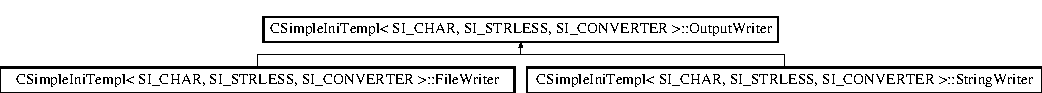
\includegraphics[height=1.244444cm]{a00030}
\end{center}
\end{figure}
\subsection*{Public Member Functions}
\begin{DoxyCompactItemize}
\item 
\hypertarget{a00030_a48e5905a9defbe96d14f3068a383463d}{}virtual void {\bfseries Write} (const char $\ast$a\+\_\+p\+Buf)=0\label{a00030_a48e5905a9defbe96d14f3068a383463d}

\end{DoxyCompactItemize}


\subsection{Detailed Description}
\subsubsection*{template$<$class S\+I\+\_\+\+C\+H\+A\+R, class S\+I\+\_\+\+S\+T\+R\+L\+E\+S\+S, class S\+I\+\_\+\+C\+O\+N\+V\+E\+R\+T\+E\+R$>$class C\+Simple\+Ini\+Templ$<$ S\+I\+\_\+\+C\+H\+A\+R, S\+I\+\_\+\+S\+T\+R\+L\+E\+S\+S, S\+I\+\_\+\+C\+O\+N\+V\+E\+R\+T\+E\+R $>$\+::\+Output\+Writer}

interface definition for the \hyperlink{a00030}{Output\+Writer} object to pass to \hyperlink{a00011_a5fea5d590edbb5eef694991c7c355915}{Save()} in order to output the I\+N\+I file data. 

The documentation for this class was generated from the following file\+:\begin{DoxyCompactItemize}
\item 
Simple\+Ini.\+h\end{DoxyCompactItemize}

\hypertarget{a00031}{}\section{fire\+:\+:String\+Caster$<$ double $>$ Struct Template Reference}
\label{a00031}\index{fire\+::\+String\+Caster$<$ double $>$@{fire\+::\+String\+Caster$<$ double $>$}}


{\ttfamily \#include $<$String\+Caster.\+h$>$}

\subsection*{Static Public Member Functions}
\begin{DoxyCompactItemize}
\item 
static double {\bfseries cast} (const string \&value)\hypertarget{a00031_a19d0552b656a96820deb3b8db8504340}{}\label{a00031_a19d0552b656a96820deb3b8db8504340}

\end{DoxyCompactItemize}


\subsection{Detailed Description}
\subsubsection*{template$<$$>$\\*
struct fire\+::\+String\+Caster$<$ double $>$}

Implementation of \hyperlink{a00029}{String\+Caster} for doubles 

The documentation for this struct was generated from the following file\+:\begin{DoxyCompactItemize}
\item 
String\+Caster.\+h\end{DoxyCompactItemize}

\hypertarget{a00032}{}\section{fire\+:\+:Provider\+Builder Struct Reference}
\label{a00032}\index{fire\+::\+Provider\+Builder@{fire\+::\+Provider\+Builder}}


{\ttfamily \#include $<$Tensor\+Provider.\+hpp$>$}

Inheritance diagram for fire\+:\+:Provider\+Builder\+:\begin{figure}[H]
\begin{center}
\leavevmode
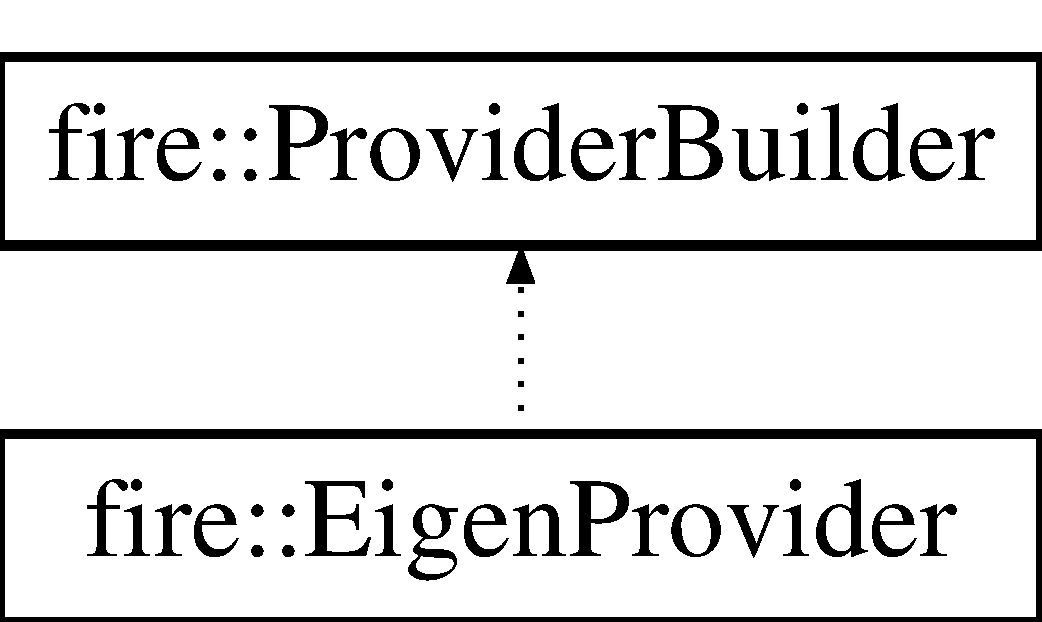
\includegraphics[height=2.000000cm]{a00032}
\end{center}
\end{figure}


\subsection{Detailed Description}
A placeholder to ensure that clients give the \hyperlink{a00046}{Tensor} an appropriate \hyperlink{a00047}{Tensor\+Provider} Builder. 

The documentation for this struct was generated from the following file\+:\begin{DoxyCompactItemize}
\item 
Tensor\+Provider.\+hpp\end{DoxyCompactItemize}

\hypertarget{a00033}{}\section{fire\+:\+:String\+Caster$<$ int $>$ Struct Template Reference}
\label{a00033}\index{fire\+::\+String\+Caster$<$ int $>$@{fire\+::\+String\+Caster$<$ int $>$}}


{\ttfamily \#include $<$String\+Caster.\+h$>$}

\subsection*{Static Public Member Functions}
\begin{DoxyCompactItemize}
\item 
static double {\bfseries cast} (const string \&value)\hypertarget{a00033_a62373040bdd4acb9e2c890d83829e22f}{}\label{a00033_a62373040bdd4acb9e2c890d83829e22f}

\end{DoxyCompactItemize}


\subsection{Detailed Description}
\subsubsection*{template$<$$>$\\*
struct fire\+::\+String\+Caster$<$ int $>$}

Implementation of \hyperlink{a00029}{String\+Caster} for ints 

The documentation for this struct was generated from the following file\+:\begin{DoxyCompactItemize}
\item 
String\+Caster.\+h\end{DoxyCompactItemize}

\hypertarget{a00034}{}\section{C\+Simple\+Ini\+Templ$<$ S\+I\+\_\+\+C\+H\+AR, S\+I\+\_\+\+S\+T\+R\+L\+E\+SS, S\+I\+\_\+\+C\+O\+N\+V\+E\+R\+T\+ER $>$\+:\+:String\+Writer Class Reference}
\label{a00034}\index{C\+Simple\+Ini\+Templ$<$ S\+I\+\_\+\+C\+H\+A\+R, S\+I\+\_\+\+S\+T\+R\+L\+E\+S\+S, S\+I\+\_\+\+C\+O\+N\+V\+E\+R\+T\+E\+R $>$\+::\+String\+Writer@{C\+Simple\+Ini\+Templ$<$ S\+I\+\_\+\+C\+H\+A\+R, S\+I\+\_\+\+S\+T\+R\+L\+E\+S\+S, S\+I\+\_\+\+C\+O\+N\+V\+E\+R\+T\+E\+R $>$\+::\+String\+Writer}}


{\ttfamily \#include $<$Simple\+Ini.\+h$>$}

Inheritance diagram for C\+Simple\+Ini\+Templ$<$ S\+I\+\_\+\+C\+H\+AR, S\+I\+\_\+\+S\+T\+R\+L\+E\+SS, S\+I\+\_\+\+C\+O\+N\+V\+E\+R\+T\+ER $>$\+:\+:String\+Writer\+:\begin{figure}[H]
\begin{center}
\leavevmode
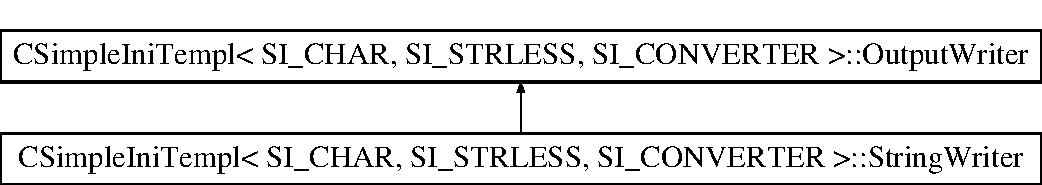
\includegraphics[height=2.000000cm]{a00034}
\end{center}
\end{figure}
\subsection*{Public Member Functions}
\begin{DoxyCompactItemize}
\item 
{\bfseries String\+Writer} (std\+::string \&a\+\_\+string)\hypertarget{a00034_ad50338a07a9b6de7e4a78d0bbc11f67b}{}\label{a00034_ad50338a07a9b6de7e4a78d0bbc11f67b}

\item 
void {\bfseries Write} (const char $\ast$a\+\_\+p\+Buf)\hypertarget{a00034_afdfd0dfe71278ea7490a9d4ef6bffadc}{}\label{a00034_afdfd0dfe71278ea7490a9d4ef6bffadc}

\end{DoxyCompactItemize}


\subsection{Detailed Description}
\subsubsection*{template$<$class S\+I\+\_\+\+C\+H\+AR, class S\+I\+\_\+\+S\+T\+R\+L\+E\+SS, class S\+I\+\_\+\+C\+O\+N\+V\+E\+R\+T\+ER$>$\\*
class C\+Simple\+Ini\+Templ$<$ S\+I\+\_\+\+C\+H\+A\+R, S\+I\+\_\+\+S\+T\+R\+L\+E\+S\+S, S\+I\+\_\+\+C\+O\+N\+V\+E\+R\+T\+E\+R $>$\+::\+String\+Writer}

\hyperlink{a00020}{Output\+Writer} class to write the I\+NI data to a string 

The documentation for this class was generated from the following file\+:\begin{DoxyCompactItemize}
\item 
Simple\+Ini.\+h\end{DoxyCompactItemize}

\hypertarget{a00035}{}\section{S\+I\+\_\+\+Convert\+A$<$ S\+I\+\_\+\+C\+H\+A\+R $>$ Class Template Reference}
\label{a00035}\index{S\+I\+\_\+\+Convert\+A$<$ S\+I\+\_\+\+C\+H\+A\+R $>$@{S\+I\+\_\+\+Convert\+A$<$ S\+I\+\_\+\+C\+H\+A\+R $>$}}


{\ttfamily \#include $<$Simple\+Ini.\+h$>$}

\subsection*{Public Member Functions}
\begin{DoxyCompactItemize}
\item 
\hypertarget{a00035_ab9c32530dc603974c3fdca06aad5b801}{}{\bfseries S\+I\+\_\+\+Convert\+A} (bool a\+\_\+b\+Store\+Is\+Utf8)\label{a00035_ab9c32530dc603974c3fdca06aad5b801}

\item 
\hypertarget{a00035_a532fa9943ae417518e370a489bdea0f5}{}{\bfseries S\+I\+\_\+\+Convert\+A} (const \hyperlink{a00035}{S\+I\+\_\+\+Convert\+A} \&rhs)\label{a00035_a532fa9943ae417518e370a489bdea0f5}

\item 
\hypertarget{a00035_a4296011c45379c08309ce2b0709b387b}{}\hyperlink{a00035}{S\+I\+\_\+\+Convert\+A} \& {\bfseries operator=} (const \hyperlink{a00035}{S\+I\+\_\+\+Convert\+A} \&rhs)\label{a00035_a4296011c45379c08309ce2b0709b387b}

\item 
size\+\_\+t \hyperlink{a00035_a30ce0eee2556184d41130311d3c8cc84}{Size\+From\+Store} (const char $\ast$a\+\_\+p\+Input\+Data, size\+\_\+t a\+\_\+u\+Input\+Data\+Len)
\item 
bool \hyperlink{a00035_a5176a6dc2dc6482280e9a08dd3607f9e}{Convert\+From\+Store} (const char $\ast$a\+\_\+p\+Input\+Data, size\+\_\+t a\+\_\+u\+Input\+Data\+Len, S\+I\+\_\+\+C\+H\+A\+R $\ast$a\+\_\+p\+Output\+Data, size\+\_\+t a\+\_\+u\+Output\+Data\+Size)
\item 
size\+\_\+t \hyperlink{a00035_a39e7a8c49712c295b24ff2ae788c01c5}{Size\+To\+Store} (const S\+I\+\_\+\+C\+H\+A\+R $\ast$a\+\_\+p\+Input\+Data)
\item 
bool \hyperlink{a00035_a188fd6d6fcba6ba8d769e70e5fbea742}{Convert\+To\+Store} (const S\+I\+\_\+\+C\+H\+A\+R $\ast$a\+\_\+p\+Input\+Data, char $\ast$a\+\_\+p\+Output\+Data, size\+\_\+t a\+\_\+u\+Output\+Data\+Size)
\end{DoxyCompactItemize}


\subsection{Detailed Description}
\subsubsection*{template$<$class S\+I\+\_\+\+C\+H\+A\+R$>$class S\+I\+\_\+\+Convert\+A$<$ S\+I\+\_\+\+C\+H\+A\+R $>$}

Null conversion class for M\+B\+C\+S/\+U\+T\+F-\/8 to char (or equivalent). 

\subsection{Member Function Documentation}
\hypertarget{a00035_a5176a6dc2dc6482280e9a08dd3607f9e}{}\index{S\+I\+\_\+\+Convert\+A@{S\+I\+\_\+\+Convert\+A}!Convert\+From\+Store@{Convert\+From\+Store}}
\index{Convert\+From\+Store@{Convert\+From\+Store}!S\+I\+\_\+\+Convert\+A@{S\+I\+\_\+\+Convert\+A}}
\subsubsection[{Convert\+From\+Store(const char $\ast$a\+\_\+p\+Input\+Data, size\+\_\+t a\+\_\+u\+Input\+Data\+Len, S\+I\+\_\+\+C\+H\+A\+R $\ast$a\+\_\+p\+Output\+Data, size\+\_\+t a\+\_\+u\+Output\+Data\+Size)}]{\setlength{\rightskip}{0pt plus 5cm}template$<$class S\+I\+\_\+\+C\+H\+A\+R $>$ bool {\bf S\+I\+\_\+\+Convert\+A}$<$ S\+I\+\_\+\+C\+H\+A\+R $>$\+::Convert\+From\+Store (
\begin{DoxyParamCaption}
\item[{const char $\ast$}]{a\+\_\+p\+Input\+Data, }
\item[{size\+\_\+t}]{a\+\_\+u\+Input\+Data\+Len, }
\item[{S\+I\+\_\+\+C\+H\+A\+R $\ast$}]{a\+\_\+p\+Output\+Data, }
\item[{size\+\_\+t}]{a\+\_\+u\+Output\+Data\+Size}
\end{DoxyParamCaption}
)\hspace{0.3cm}{\ttfamily [inline]}}\label{a00035_a5176a6dc2dc6482280e9a08dd3607f9e}
Convert the input string from the storage format to S\+I\+\_\+\+C\+H\+A\+R. The storage format is always U\+T\+F-\/8 or M\+B\+C\+S.


\begin{DoxyParams}{Parameters}
{\em a\+\_\+p\+Input\+Data} & Data in storage format to be converted to S\+I\+\_\+\+C\+H\+A\+R. \\
\hline
{\em a\+\_\+u\+Input\+Data\+Len} & Length of storage format data in bytes. This must be the actual length of the data, including N\+U\+L\+L byte if N\+U\+L\+L terminated string is required. \\
\hline
{\em a\+\_\+p\+Output\+Data} & Pointer to the output buffer to received the converted data. \\
\hline
{\em a\+\_\+u\+Output\+Data\+Size} & Size of the output buffer in S\+I\+\_\+\+C\+H\+A\+R. \\
\hline
\end{DoxyParams}
\begin{DoxyReturn}{Returns}
true if all of the input data was successfully converted. 
\end{DoxyReturn}
\hypertarget{a00035_a188fd6d6fcba6ba8d769e70e5fbea742}{}\index{S\+I\+\_\+\+Convert\+A@{S\+I\+\_\+\+Convert\+A}!Convert\+To\+Store@{Convert\+To\+Store}}
\index{Convert\+To\+Store@{Convert\+To\+Store}!S\+I\+\_\+\+Convert\+A@{S\+I\+\_\+\+Convert\+A}}
\subsubsection[{Convert\+To\+Store(const S\+I\+\_\+\+C\+H\+A\+R $\ast$a\+\_\+p\+Input\+Data, char $\ast$a\+\_\+p\+Output\+Data, size\+\_\+t a\+\_\+u\+Output\+Data\+Size)}]{\setlength{\rightskip}{0pt plus 5cm}template$<$class S\+I\+\_\+\+C\+H\+A\+R $>$ bool {\bf S\+I\+\_\+\+Convert\+A}$<$ S\+I\+\_\+\+C\+H\+A\+R $>$\+::Convert\+To\+Store (
\begin{DoxyParamCaption}
\item[{const S\+I\+\_\+\+C\+H\+A\+R $\ast$}]{a\+\_\+p\+Input\+Data, }
\item[{char $\ast$}]{a\+\_\+p\+Output\+Data, }
\item[{size\+\_\+t}]{a\+\_\+u\+Output\+Data\+Size}
\end{DoxyParamCaption}
)\hspace{0.3cm}{\ttfamily [inline]}}\label{a00035_a188fd6d6fcba6ba8d769e70e5fbea742}
Convert the input string to the storage format of this data. The storage format is always U\+T\+F-\/8 or M\+B\+C\+S.


\begin{DoxyParams}{Parameters}
{\em a\+\_\+p\+Input\+Data} & N\+U\+L\+L terminated source string to convert. All of the data will be converted including the terminating N\+U\+L\+L character. \\
\hline
{\em a\+\_\+p\+Output\+Data} & Pointer to the buffer to receive the converted string. \\
\hline
{\em a\+\_\+u\+Output\+Data\+Size} & Size of the output buffer in char. \\
\hline
\end{DoxyParams}
\begin{DoxyReturn}{Returns}
true if all of the input data, including the terminating N\+U\+L\+L character was successfully converted. 
\end{DoxyReturn}
\hypertarget{a00035_a30ce0eee2556184d41130311d3c8cc84}{}\index{S\+I\+\_\+\+Convert\+A@{S\+I\+\_\+\+Convert\+A}!Size\+From\+Store@{Size\+From\+Store}}
\index{Size\+From\+Store@{Size\+From\+Store}!S\+I\+\_\+\+Convert\+A@{S\+I\+\_\+\+Convert\+A}}
\subsubsection[{Size\+From\+Store(const char $\ast$a\+\_\+p\+Input\+Data, size\+\_\+t a\+\_\+u\+Input\+Data\+Len)}]{\setlength{\rightskip}{0pt plus 5cm}template$<$class S\+I\+\_\+\+C\+H\+A\+R $>$ size\+\_\+t {\bf S\+I\+\_\+\+Convert\+A}$<$ S\+I\+\_\+\+C\+H\+A\+R $>$\+::Size\+From\+Store (
\begin{DoxyParamCaption}
\item[{const char $\ast$}]{a\+\_\+p\+Input\+Data, }
\item[{size\+\_\+t}]{a\+\_\+u\+Input\+Data\+Len}
\end{DoxyParamCaption}
)\hspace{0.3cm}{\ttfamily [inline]}}\label{a00035_a30ce0eee2556184d41130311d3c8cc84}
Calculate the number of S\+I\+\_\+\+C\+H\+A\+R required for converting the input from the storage format. The storage format is always U\+T\+F-\/8 or M\+B\+C\+S.


\begin{DoxyParams}{Parameters}
{\em a\+\_\+p\+Input\+Data} & Data in storage format to be converted to S\+I\+\_\+\+C\+H\+A\+R. \\
\hline
{\em a\+\_\+u\+Input\+Data\+Len} & Length of storage format data in bytes. This must be the actual length of the data, including N\+U\+L\+L byte if N\+U\+L\+L terminated string is required. \\
\hline
\end{DoxyParams}
\begin{DoxyReturn}{Returns}
Number of S\+I\+\_\+\+C\+H\+A\+R required by the string when converted. If there are embedded N\+U\+L\+L bytes in the input data, only the string up and not including the N\+U\+L\+L byte will be converted. 

-\/1 cast to size\+\_\+t on a conversion error. 
\end{DoxyReturn}
\hypertarget{a00035_a39e7a8c49712c295b24ff2ae788c01c5}{}\index{S\+I\+\_\+\+Convert\+A@{S\+I\+\_\+\+Convert\+A}!Size\+To\+Store@{Size\+To\+Store}}
\index{Size\+To\+Store@{Size\+To\+Store}!S\+I\+\_\+\+Convert\+A@{S\+I\+\_\+\+Convert\+A}}
\subsubsection[{Size\+To\+Store(const S\+I\+\_\+\+C\+H\+A\+R $\ast$a\+\_\+p\+Input\+Data)}]{\setlength{\rightskip}{0pt plus 5cm}template$<$class S\+I\+\_\+\+C\+H\+A\+R $>$ size\+\_\+t {\bf S\+I\+\_\+\+Convert\+A}$<$ S\+I\+\_\+\+C\+H\+A\+R $>$\+::Size\+To\+Store (
\begin{DoxyParamCaption}
\item[{const S\+I\+\_\+\+C\+H\+A\+R $\ast$}]{a\+\_\+p\+Input\+Data}
\end{DoxyParamCaption}
)\hspace{0.3cm}{\ttfamily [inline]}}\label{a00035_a39e7a8c49712c295b24ff2ae788c01c5}
Calculate the number of char required by the storage format of this data. The storage format is always U\+T\+F-\/8 or M\+B\+C\+S.


\begin{DoxyParams}{Parameters}
{\em a\+\_\+p\+Input\+Data} & N\+U\+L\+L terminated string to calculate the number of bytes required to be converted to storage format. \\
\hline
\end{DoxyParams}
\begin{DoxyReturn}{Returns}
Number of bytes required by the string when converted to storage format. This size always includes space for the terminating N\+U\+L\+L character. 

-\/1 cast to size\+\_\+t on a conversion error. 
\end{DoxyReturn}


The documentation for this class was generated from the following file\+:\begin{DoxyCompactItemize}
\item 
Simple\+Ini.\+h\end{DoxyCompactItemize}

\hypertarget{a00036}{}\section{Test\+Struct Struct Reference}
\label{a00036}\index{Test\+Struct@{Test\+Struct}}
\subsection*{Public Member Functions}
\begin{DoxyCompactItemize}
\item 
{\bfseries Test\+Struct} (int value)\hypertarget{a00036_ad1b28d11092e7dcf1818901f7a276120}{}\label{a00036_ad1b28d11092e7dcf1818901f7a276120}

\end{DoxyCompactItemize}
\subsection*{Public Attributes}
\begin{DoxyCompactItemize}
\item 
int {\bfseries A}\hypertarget{a00036_a948fae89410671cffc8087f752a45552}{}\label{a00036_a948fae89410671cffc8087f752a45552}

\end{DoxyCompactItemize}


\subsection{Detailed Description}
A simple test struct for the tests. 

The documentation for this struct was generated from the following file\+:\begin{DoxyCompactItemize}
\item 
Build\+Test.\+cpp\end{DoxyCompactItemize}

\hypertarget{a00037}{}\section{S\+I\+\_\+\+Generic\+Case$<$ S\+I\+\_\+\+C\+H\+A\+R $>$ Struct Template Reference}
\label{a00037}\index{S\+I\+\_\+\+Generic\+Case$<$ S\+I\+\_\+\+C\+H\+A\+R $>$@{S\+I\+\_\+\+Generic\+Case$<$ S\+I\+\_\+\+C\+H\+A\+R $>$}}


{\ttfamily \#include $<$Simple\+Ini.\+h$>$}

\subsection*{Public Member Functions}
\begin{DoxyCompactItemize}
\item 
\hypertarget{a00037_af91c0d1b328b5c1bd15053204dcfa9b1}{}bool {\bfseries operator()} (const S\+I\+\_\+\+C\+H\+A\+R $\ast$p\+Left, const S\+I\+\_\+\+C\+H\+A\+R $\ast$p\+Right) const \label{a00037_af91c0d1b328b5c1bd15053204dcfa9b1}

\end{DoxyCompactItemize}


\subsection{Detailed Description}
\subsubsection*{template$<$class S\+I\+\_\+\+C\+H\+A\+R$>$struct S\+I\+\_\+\+Generic\+Case$<$ S\+I\+\_\+\+C\+H\+A\+R $>$}

Generic case-\/sensitive less than comparison. This class returns numerically ordered A\+S\+C\+I\+I case-\/sensitive text for all possible sizes and types of S\+I\+\_\+\+C\+H\+A\+R. 

The documentation for this struct was generated from the following file\+:\begin{DoxyCompactItemize}
\item 
Simple\+Ini.\+h\end{DoxyCompactItemize}

%--- End generated contents ---

% Index
\backmatter
\newpage
\phantomsection
\clearemptydoublepage
\addcontentsline{toc}{chapter}{Index}
\printindex

\end{document}
